\documentclass{book}
\usepackage[a4paper,top=2.5cm,bottom=2.5cm,left=2.5cm,right=2.5cm]{geometry}
\usepackage{makeidx}
\usepackage{natbib}
\usepackage{graphicx}
\usepackage{multicol}
\usepackage{float}
\usepackage{listings}
\usepackage{color}
\usepackage{ifthen}
\usepackage[table]{xcolor}
\usepackage{textcomp}
\usepackage{alltt}
\usepackage{ifpdf}
\ifpdf
\usepackage[pdftex,
            pagebackref=true,
            colorlinks=true,
            linkcolor=blue,
            unicode
           ]{hyperref}
\else
\usepackage[ps2pdf,
            pagebackref=true,
            colorlinks=true,
            linkcolor=blue,
            unicode
           ]{hyperref}
\usepackage{pspicture}
\fi
\usepackage[utf8]{inputenc}
\usepackage{mathptmx}
\usepackage[scaled=.90]{helvet}
\usepackage{courier}
\usepackage{sectsty}
\usepackage{amssymb}
\usepackage[titles]{tocloft}
\usepackage{doxygen}
\lstset{language=C++,inputencoding=utf8,basicstyle=\footnotesize,breaklines=true,breakatwhitespace=true,tabsize=4,numbers=left }
\makeindex
\setcounter{tocdepth}{3}
\renewcommand{\footrulewidth}{0.4pt}
\renewcommand{\familydefault}{\sfdefault}
\hfuzz=15pt
\setlength{\emergencystretch}{15pt}
\hbadness=750
\tolerance=750
\begin{document}
\hypersetup{pageanchor=false,citecolor=blue}
\begin{titlepage}
\vspace*{7cm}
\begin{center}
{\Large Ensemble Clustering }\\
\vspace*{1cm}
{\large Generated by Doxygen 1.8.2}\\
\vspace*{0.5cm}
{\small Thu Dec 13 2012 16:27:32}\\
\end{center}
\end{titlepage}
\clearemptydoublepage
\pagenumbering{roman}
\tableofcontents
\clearemptydoublepage
\pagenumbering{arabic}
\hypersetup{pageanchor=true,citecolor=blue}
\chapter{Namespace Index}
\section{Namespace List}
Here is a list of all namespaces with brief descriptions\-:\begin{DoxyCompactList}
\item\contentsline{section}{\hyperlink{namespace_aux}{Aux} }{\pageref{namespace_aux}}{}
\item\contentsline{section}{\hyperlink{namespace_networ_kit}{Networ\-Kit} }{\pageref{namespace_networ_kit}}{}
\item\contentsline{section}{\hyperlink{namespace_option_parser}{Option\-Parser} \\*The namespace of The Lean Mean C++ \hyperlink{class_option_parser_1_1_option}{Option} \hyperlink{class_option_parser_1_1_parser}{Parser} }{\pageref{namespace_option_parser}}{}
\end{DoxyCompactList}

\chapter{Hierarchical Index}
\section{Class Hierarchy}
This inheritance list is sorted roughly, but not completely, alphabetically\-:\begin{DoxyCompactList}
\item \contentsline{section}{Option\-Parser\-:\-:Parser\-:\-:Action}{\pageref{struct_option_parser_1_1_parser_1_1_action}}{}
\begin{DoxyCompactList}
\item \contentsline{section}{Option\-Parser\-:\-:Parser\-:\-:Store\-Option\-Action}{\pageref{class_option_parser_1_1_parser_1_1_store_option_action}}{}
\item \contentsline{section}{Option\-Parser\-:\-:Stats\-:\-:Count\-Options\-Action}{\pageref{class_option_parser_1_1_stats_1_1_count_options_action}}{}
\end{DoxyCompactList}
\item \contentsline{section}{Option\-Parser\-:\-:Arg}{\pageref{struct_option_parser_1_1_arg}}{}
\begin{DoxyCompactList}
\item \contentsline{section}{Arg}{\pageref{class_arg}}{}
\end{DoxyCompactList}
\item \contentsline{section}{Networ\-Kit\-:\-:Clusterer}{\pageref{class_networ_kit_1_1_clusterer}}{}
\begin{DoxyCompactList}
\item \contentsline{section}{Networ\-Kit\-:\-:Ensemble\-Multilevel}{\pageref{class_networ_kit_1_1_ensemble_multilevel}}{}
\item \contentsline{section}{Networ\-Kit\-:\-:Ensemble\-Preprocessing}{\pageref{class_networ_kit_1_1_ensemble_preprocessing}}{}
\item \contentsline{section}{Networ\-Kit\-:\-:Label\-Propagation}{\pageref{class_networ_kit_1_1_label_propagation}}{}
\item \contentsline{section}{Networ\-Kit\-:\-:Louvain}{\pageref{class_networ_kit_1_1_louvain}}{}
\item \contentsline{section}{Networ\-Kit\-:\-:Parallel\-Agglomerative\-Clusterer}{\pageref{class_networ_kit_1_1_parallel_agglomerative_clusterer}}{}
\item \contentsline{section}{Networ\-Kit\-:\-:Random\-Clusterer}{\pageref{class_networ_kit_1_1_random_clusterer}}{}
\end{DoxyCompactList}
\item \contentsline{section}{Networ\-Kit\-:\-:Clustering\-Generator}{\pageref{class_networ_kit_1_1_clustering_generator}}{}
\item \contentsline{section}{Networ\-Kit\-:\-:Clustering\-Projector}{\pageref{class_networ_kit_1_1_clustering_projector}}{}
\item \contentsline{section}{Networ\-Kit\-:\-:Clustering\-Reader}{\pageref{class_networ_kit_1_1_clustering_reader}}{}
\item \contentsline{section}{Networ\-Kit\-:\-:Clustering\-Writer}{\pageref{class_networ_kit_1_1_clustering_writer}}{}
\item \contentsline{section}{Networ\-Kit\-:\-:Contracter}{\pageref{class_networ_kit_1_1_contracter}}{}
\begin{DoxyCompactList}
\item \contentsline{section}{Networ\-Kit\-:\-:Cluster\-Contracter}{\pageref{class_networ_kit_1_1_cluster_contracter}}{}
\item \contentsline{section}{Networ\-Kit\-:\-:Matching\-Contracter}{\pageref{class_networ_kit_1_1_matching_contracter}}{}
\end{DoxyCompactList}
\item \contentsline{section}{C\-S\-V\-Writer}{\pageref{class_c_s_v_writer}}{}
\item \contentsline{section}{Option\-Parser\-:\-:Descriptor}{\pageref{struct_option_parser_1_1_descriptor}}{}
\item \contentsline{section}{Networ\-Kit\-:\-:Dissimilarity\-Measure}{\pageref{class_networ_kit_1_1_dissimilarity_measure}}{}
\begin{DoxyCompactList}
\item \contentsline{section}{Networ\-Kit\-:\-:Jaccard\-Measure}{\pageref{class_networ_kit_1_1_jaccard_measure}}{}
\item \contentsline{section}{Networ\-Kit\-:\-:Rand\-Measure}{\pageref{class_networ_kit_1_1_rand_measure}}{}
\end{DoxyCompactList}
\item \contentsline{section}{Networ\-Kit\-:\-:Graph\-:\-:Edge\-Attribute}{\pageref{class_networ_kit_1_1_graph_1_1_edge_attribute}}{}
\item \contentsline{section}{Networ\-Kit\-:\-:Edge\-Scoring$<$ T $>$}{\pageref{class_networ_kit_1_1_edge_scoring}}{}
\begin{DoxyCompactList}
\item \contentsline{section}{Networ\-Kit\-:\-:Modularity\-Scoring$<$ T $>$}{\pageref{class_networ_kit_1_1_modularity_scoring}}{}
\end{DoxyCompactList}
\item \contentsline{section}{Networ\-Kit\-:\-:Graph}{\pageref{class_networ_kit_1_1_graph}}{}
\item \contentsline{section}{Networ\-Kit\-:\-:Graph\-Contraction}{\pageref{class_networ_kit_1_1_graph_contraction}}{}
\item \contentsline{section}{Networ\-Kit\-:\-:Graph\-Generator}{\pageref{class_networ_kit_1_1_graph_generator}}{}
\item \contentsline{section}{Networ\-Kit\-:\-:Graph\-I\-O}{\pageref{class_networ_kit_1_1_graph_i_o}}{}
\item \contentsline{section}{Networ\-Kit\-:\-:Graph\-Reader}{\pageref{class_networ_kit_1_1_graph_reader}}{}
\begin{DoxyCompactList}
\item \contentsline{section}{Networ\-Kit\-:\-:M\-E\-T\-I\-S\-Graph\-Reader}{\pageref{class_networ_kit_1_1_m_e_t_i_s_graph_reader}}{}
\end{DoxyCompactList}
\item \contentsline{section}{Networ\-Kit\-:\-:Graph\-Writer}{\pageref{class_networ_kit_1_1_graph_writer}}{}
\begin{DoxyCompactList}
\item \contentsline{section}{Networ\-Kit\-:\-:M\-E\-T\-I\-S\-Graph\-Writer}{\pageref{class_networ_kit_1_1_m_e_t_i_s_graph_writer}}{}
\end{DoxyCompactList}
\item \contentsline{section}{Networ\-Kit\-:\-:Independent\-Set\-Finder}{\pageref{class_networ_kit_1_1_independent_set_finder}}{}
\begin{DoxyCompactList}
\item \contentsline{section}{Networ\-Kit\-:\-:Luby}{\pageref{class_networ_kit_1_1_luby}}{}
\end{DoxyCompactList}
\item \contentsline{section}{Networ\-Kit\-:\-:Index\-Map$<$ I, T $>$}{\pageref{class_networ_kit_1_1_index_map}}{}
\item \contentsline{section}{Networ\-Kit\-:\-:Index\-Map$<$ node, cluster $>$}{\pageref{class_networ_kit_1_1_index_map}}{}
\begin{DoxyCompactList}
\item \contentsline{section}{Networ\-Kit\-:\-:Node\-Map$<$ cluster $>$}{\pageref{class_networ_kit_1_1_node_map}}{}
\begin{DoxyCompactList}
\item \contentsline{section}{Networ\-Kit\-:\-:Clustering}{\pageref{class_networ_kit_1_1_clustering}}{}
\end{DoxyCompactList}
\end{DoxyCompactList}
\item \contentsline{section}{Networ\-Kit\-:\-:Index\-Map$<$ node, node $>$}{\pageref{class_networ_kit_1_1_index_map}}{}
\begin{DoxyCompactList}
\item \contentsline{section}{Networ\-Kit\-:\-:Node\-Map$<$ node $>$}{\pageref{class_networ_kit_1_1_node_map}}{}
\begin{DoxyCompactList}
\item \contentsline{section}{Networ\-Kit\-:\-:Matching}{\pageref{class_networ_kit_1_1_matching}}{}
\end{DoxyCompactList}
\end{DoxyCompactList}
\item \contentsline{section}{Networ\-Kit\-:\-:Index\-Map$<$ node, T $>$}{\pageref{class_networ_kit_1_1_index_map}}{}
\begin{DoxyCompactList}
\item \contentsline{section}{Networ\-Kit\-:\-:Node\-Map$<$ T $>$}{\pageref{class_networ_kit_1_1_node_map}}{}
\end{DoxyCompactList}
\item \contentsline{section}{Option\-Parser\-:\-:Print\-Usage\-Implementation\-:\-:I\-String\-Writer}{\pageref{struct_option_parser_1_1_print_usage_implementation_1_1_i_string_writer}}{}
\begin{DoxyCompactList}
\item \contentsline{section}{Option\-Parser\-:\-:Print\-Usage\-Implementation\-:\-:Function\-Writer$<$ Function $>$}{\pageref{struct_option_parser_1_1_print_usage_implementation_1_1_function_writer}}{}
\item \contentsline{section}{Option\-Parser\-:\-:Print\-Usage\-Implementation\-:\-:O\-Stream\-Writer$<$ O\-Stream $>$}{\pageref{struct_option_parser_1_1_print_usage_implementation_1_1_o_stream_writer}}{}
\item \contentsline{section}{Option\-Parser\-:\-:Print\-Usage\-Implementation\-:\-:Stream\-Writer$<$ Function, Stream $>$}{\pageref{struct_option_parser_1_1_print_usage_implementation_1_1_stream_writer}}{}
\item \contentsline{section}{Option\-Parser\-:\-:Print\-Usage\-Implementation\-:\-:Syscall\-Writer$<$ Syscall $>$}{\pageref{struct_option_parser_1_1_print_usage_implementation_1_1_syscall_writer}}{}
\item \contentsline{section}{Option\-Parser\-:\-:Print\-Usage\-Implementation\-:\-:Temporary\-Writer$<$ Temporary $>$}{\pageref{struct_option_parser_1_1_print_usage_implementation_1_1_temporary_writer}}{}
\end{DoxyCompactList}
\item \contentsline{section}{Option\-Parser\-:\-:Print\-Usage\-Implementation\-:\-:Line\-Part\-Iterator}{\pageref{class_option_parser_1_1_print_usage_implementation_1_1_line_part_iterator}}{}
\item \contentsline{section}{Option\-Parser\-:\-:Print\-Usage\-Implementation\-:\-:Line\-Wrapper}{\pageref{class_option_parser_1_1_print_usage_implementation_1_1_line_wrapper}}{}
\item \contentsline{section}{Networ\-Kit\-:\-:Matcher}{\pageref{class_networ_kit_1_1_matcher}}{}
\begin{DoxyCompactList}
\item \contentsline{section}{Networ\-Kit\-:\-:Parallel\-Matcher}{\pageref{class_networ_kit_1_1_parallel_matcher}}{}
\end{DoxyCompactList}
\item \contentsline{section}{Networ\-Kit\-:\-:M\-E\-T\-I\-S\-Parser}{\pageref{class_networ_kit_1_1_m_e_t_i_s_parser}}{}
\item \contentsline{section}{Networ\-Kit\-:\-:Graph\-:\-:Node\-Attribute}{\pageref{class_networ_kit_1_1_graph_1_1_node_attribute}}{}
\item \contentsline{section}{Node\-Map$<$ T $>$}{\pageref{class_node_map}}{}
\item \contentsline{section}{Noise}{\pageref{class_noise}}{}
\item \contentsline{section}{Networ\-Kit\-:\-:Numeric\-Tools}{\pageref{class_networ_kit_1_1_numeric_tools}}{}
\item \contentsline{section}{Option\-Parser\-:\-:Option}{\pageref{class_option_parser_1_1_option}}{}
\item \contentsline{section}{Networ\-Kit\-:\-:Overlapper}{\pageref{class_networ_kit_1_1_overlapper}}{}
\begin{DoxyCompactList}
\item \contentsline{section}{Networ\-Kit\-:\-:Hashing\-Overlapper}{\pageref{class_networ_kit_1_1_hashing_overlapper}}{}
\item \contentsline{section}{Networ\-Kit\-:\-:Region\-Growing\-Overlapper}{\pageref{class_networ_kit_1_1_region_growing_overlapper}}{}
\end{DoxyCompactList}
\item \contentsline{section}{Option\-Parser\-:\-:Parser}{\pageref{class_option_parser_1_1_parser}}{}
\item \contentsline{section}{Option\-Parser\-:\-:Print\-Usage\-Implementation}{\pageref{struct_option_parser_1_1_print_usage_implementation}}{}
\item \contentsline{section}{Aux\-:\-:Progress\-Meter}{\pageref{class_aux_1_1_progress_meter}}{}
\item \contentsline{section}{Networ\-Kit\-:\-:Quality\-Measure}{\pageref{class_networ_kit_1_1_quality_measure}}{}
\begin{DoxyCompactList}
\item \contentsline{section}{Networ\-Kit\-:\-:Coverage}{\pageref{class_networ_kit_1_1_coverage}}{}
\item \contentsline{section}{Networ\-Kit\-:\-:Coverage\-Sequential}{\pageref{class_networ_kit_1_1_coverage_sequential}}{}
\item \contentsline{section}{Networ\-Kit\-:\-:Modularity}{\pageref{class_networ_kit_1_1_modularity}}{}
\item \contentsline{section}{Networ\-Kit\-:\-:Modularity\-Sequential}{\pageref{class_networ_kit_1_1_modularity_sequential}}{}
\end{DoxyCompactList}
\item \contentsline{section}{Aux\-:\-:Random\-Integer}{\pageref{class_aux_1_1_random_integer}}{}
\item \contentsline{section}{Aux\-:\-:Random\-Probability}{\pageref{class_aux_1_1_random_probability}}{}
\item \contentsline{section}{Option\-Parser\-:\-:Stats}{\pageref{struct_option_parser_1_1_stats}}{}
\item \contentsline{section}{Aux\-:\-:String\-Tools}{\pageref{class_aux_1_1_string_tools}}{}
\item Test\begin{DoxyCompactList}
\item \contentsline{section}{Aux\-G\-Test}{\pageref{class_aux_g_test}}{}
\item \contentsline{section}{Networ\-Kit\-:\-:Basics\-Benchmark}{\pageref{class_networ_kit_1_1_basics_benchmark}}{}
\item \contentsline{section}{Networ\-Kit\-:\-:Clustering\-Algo\-G\-Test}{\pageref{class_networ_kit_1_1_clustering_algo_g_test}}{}
\item \contentsline{section}{Networ\-Kit\-:\-:Clustering\-G\-Test}{\pageref{class_networ_kit_1_1_clustering_g_test}}{}
\item \contentsline{section}{Networ\-Kit\-:\-:Coarsening\-G\-Test}{\pageref{class_networ_kit_1_1_coarsening_g_test}}{}
\item \contentsline{section}{Networ\-Kit\-:\-:Ensemble\-G\-Test}{\pageref{class_networ_kit_1_1_ensemble_g_test}}{}
\item \contentsline{section}{Networ\-Kit\-:\-:Graph2\-Benchmark}{\pageref{class_networ_kit_1_1_graph2_benchmark}}{}
\item \contentsline{section}{Networ\-Kit\-:\-:Graph2\-G\-Test}{\pageref{class_networ_kit_1_1_graph2_g_test}}{}
\item \contentsline{section}{Networ\-Kit\-:\-:Graph\-Benchmark}{\pageref{class_networ_kit_1_1_graph_benchmark}}{}
\item \contentsline{section}{Networ\-Kit\-:\-:Graph\-Generator\-G\-Test}{\pageref{class_networ_kit_1_1_graph_generator_g_test}}{}
\item \contentsline{section}{Networ\-Kit\-:\-:Graph\-G\-Test}{\pageref{class_networ_kit_1_1_graph_g_test}}{}
\item \contentsline{section}{Networ\-Kit\-:\-:Independent\-Set\-G\-Test}{\pageref{class_networ_kit_1_1_independent_set_g_test}}{}
\item \contentsline{section}{Networ\-Kit\-:\-:Input\-G\-Test}{\pageref{class_networ_kit_1_1_input_g_test}}{}
\item \contentsline{section}{Networ\-Kit\-:\-:I\-O\-Benchmark}{\pageref{class_networ_kit_1_1_i_o_benchmark}}{}
\item \contentsline{section}{Networ\-Kit\-:\-:Overlap\-G\-Test}{\pageref{class_networ_kit_1_1_overlap_g_test}}{}
\end{DoxyCompactList}
\item Test\-With\-Param\begin{DoxyCompactList}
\item \contentsline{section}{Parametrized\-G\-Test}{\pageref{class_parametrized_g_test}}{}
\end{DoxyCompactList}
\item \contentsline{section}{Aux\-:\-:Timer}{\pageref{class_aux_1_1_timer}}{}
\end{DoxyCompactList}

\chapter{Class Index}
\section{Class List}
Here are the classes, structs, unions and interfaces with brief descriptions\-:\begin{DoxyCompactList}
\item\contentsline{section}{\hyperlink{struct_option_parser_1_1_parser_1_1_action}{Option\-Parser\-::\-Parser\-::\-Action} }{\pageref{struct_option_parser_1_1_parser_1_1_action}}{}
\item\contentsline{section}{\hyperlink{class_arg}{Arg} }{\pageref{class_arg}}{}
\item\contentsline{section}{\hyperlink{struct_option_parser_1_1_arg}{Option\-Parser\-::\-Arg} \\*Functions for checking the validity of option arguments }{\pageref{struct_option_parser_1_1_arg}}{}
\item\contentsline{section}{\hyperlink{class_aux_g_test}{Aux\-G\-Test} }{\pageref{class_aux_g_test}}{}
\item\contentsline{section}{\hyperlink{class_networ_kit_1_1_basics_benchmark}{Networ\-Kit\-::\-Basics\-Benchmark} }{\pageref{class_networ_kit_1_1_basics_benchmark}}{}
\item\contentsline{section}{\hyperlink{class_networ_kit_1_1_cluster_contracter}{Networ\-Kit\-::\-Cluster\-Contracter} }{\pageref{class_networ_kit_1_1_cluster_contracter}}{}
\item\contentsline{section}{\hyperlink{class_networ_kit_1_1_clusterer}{Networ\-Kit\-::\-Clusterer} }{\pageref{class_networ_kit_1_1_clusterer}}{}
\item\contentsline{section}{\hyperlink{class_networ_kit_1_1_clustering}{Networ\-Kit\-::\-Clustering} }{\pageref{class_networ_kit_1_1_clustering}}{}
\item\contentsline{section}{\hyperlink{class_networ_kit_1_1_clustering_algo_g_test}{Networ\-Kit\-::\-Clustering\-Algo\-G\-Test} }{\pageref{class_networ_kit_1_1_clustering_algo_g_test}}{}
\item\contentsline{section}{\hyperlink{class_networ_kit_1_1_clustering_generator}{Networ\-Kit\-::\-Clustering\-Generator} }{\pageref{class_networ_kit_1_1_clustering_generator}}{}
\item\contentsline{section}{\hyperlink{class_networ_kit_1_1_clustering_g_test}{Networ\-Kit\-::\-Clustering\-G\-Test} }{\pageref{class_networ_kit_1_1_clustering_g_test}}{}
\item\contentsline{section}{\hyperlink{class_networ_kit_1_1_clustering_projector}{Networ\-Kit\-::\-Clustering\-Projector} }{\pageref{class_networ_kit_1_1_clustering_projector}}{}
\item\contentsline{section}{\hyperlink{class_networ_kit_1_1_clustering_reader}{Networ\-Kit\-::\-Clustering\-Reader} }{\pageref{class_networ_kit_1_1_clustering_reader}}{}
\item\contentsline{section}{\hyperlink{class_networ_kit_1_1_clustering_writer}{Networ\-Kit\-::\-Clustering\-Writer} }{\pageref{class_networ_kit_1_1_clustering_writer}}{}
\item\contentsline{section}{\hyperlink{class_networ_kit_1_1_coarsening_g_test}{Networ\-Kit\-::\-Coarsening\-G\-Test} \\*Googletest test fixture for the coarsening module }{\pageref{class_networ_kit_1_1_coarsening_g_test}}{}
\item\contentsline{section}{\hyperlink{class_networ_kit_1_1_contracter}{Networ\-Kit\-::\-Contracter} }{\pageref{class_networ_kit_1_1_contracter}}{}
\item\contentsline{section}{\hyperlink{class_option_parser_1_1_stats_1_1_count_options_action}{Option\-Parser\-::\-Stats\-::\-Count\-Options\-Action} }{\pageref{class_option_parser_1_1_stats_1_1_count_options_action}}{}
\item\contentsline{section}{\hyperlink{class_networ_kit_1_1_coverage}{Networ\-Kit\-::\-Coverage} }{\pageref{class_networ_kit_1_1_coverage}}{}
\item\contentsline{section}{\hyperlink{class_networ_kit_1_1_coverage_sequential}{Networ\-Kit\-::\-Coverage\-Sequential} }{\pageref{class_networ_kit_1_1_coverage_sequential}}{}
\item\contentsline{section}{\hyperlink{class_c_s_v_writer}{C\-S\-V\-Writer} }{\pageref{class_c_s_v_writer}}{}
\item\contentsline{section}{\hyperlink{struct_option_parser_1_1_descriptor}{Option\-Parser\-::\-Descriptor} \\*Describes an option, its help text (usage) and how it should be parsed }{\pageref{struct_option_parser_1_1_descriptor}}{}
\item\contentsline{section}{\hyperlink{class_networ_kit_1_1_dissimilarity_measure}{Networ\-Kit\-::\-Dissimilarity\-Measure} \\*Base class for all clustering dissimilarity measures }{\pageref{class_networ_kit_1_1_dissimilarity_measure}}{}
\item\contentsline{section}{\hyperlink{class_networ_kit_1_1_graph_1_1_edge_attribute}{Networ\-Kit\-::\-Graph\-::\-Edge\-Attribute} }{\pageref{class_networ_kit_1_1_graph_1_1_edge_attribute}}{}
\item\contentsline{section}{\hyperlink{class_networ_kit_1_1_edge_scoring}{Networ\-Kit\-::\-Edge\-Scoring$<$ T $>$} }{\pageref{class_networ_kit_1_1_edge_scoring}}{}
\item\contentsline{section}{\hyperlink{class_networ_kit_1_1_ensemble_g_test}{Networ\-Kit\-::\-Ensemble\-G\-Test} }{\pageref{class_networ_kit_1_1_ensemble_g_test}}{}
\item\contentsline{section}{\hyperlink{class_networ_kit_1_1_ensemble_multilevel}{Networ\-Kit\-::\-Ensemble\-Multilevel} }{\pageref{class_networ_kit_1_1_ensemble_multilevel}}{}
\item\contentsline{section}{\hyperlink{class_networ_kit_1_1_ensemble_preprocessing}{Networ\-Kit\-::\-Ensemble\-Preprocessing} }{\pageref{class_networ_kit_1_1_ensemble_preprocessing}}{}
\item\contentsline{section}{\hyperlink{struct_option_parser_1_1_print_usage_implementation_1_1_function_writer}{Option\-Parser\-::\-Print\-Usage\-Implementation\-::\-Function\-Writer$<$ Function $>$} }{\pageref{struct_option_parser_1_1_print_usage_implementation_1_1_function_writer}}{}
\item\contentsline{section}{\hyperlink{class_networ_kit_1_1_graph}{Networ\-Kit\-::\-Graph} }{\pageref{class_networ_kit_1_1_graph}}{}
\item\contentsline{section}{\hyperlink{class_networ_kit_1_1_graph2_benchmark}{Networ\-Kit\-::\-Graph2\-Benchmark} }{\pageref{class_networ_kit_1_1_graph2_benchmark}}{}
\item\contentsline{section}{\hyperlink{class_networ_kit_1_1_graph2_g_test}{Networ\-Kit\-::\-Graph2\-G\-Test} }{\pageref{class_networ_kit_1_1_graph2_g_test}}{}
\item\contentsline{section}{\hyperlink{class_networ_kit_1_1_graph_benchmark}{Networ\-Kit\-::\-Graph\-Benchmark} }{\pageref{class_networ_kit_1_1_graph_benchmark}}{}
\item\contentsline{section}{\hyperlink{class_networ_kit_1_1_graph_contraction}{Networ\-Kit\-::\-Graph\-Contraction} }{\pageref{class_networ_kit_1_1_graph_contraction}}{}
\item\contentsline{section}{\hyperlink{class_networ_kit_1_1_graph_generator}{Networ\-Kit\-::\-Graph\-Generator} }{\pageref{class_networ_kit_1_1_graph_generator}}{}
\item\contentsline{section}{\hyperlink{class_networ_kit_1_1_graph_generator_g_test}{Networ\-Kit\-::\-Graph\-Generator\-G\-Test} }{\pageref{class_networ_kit_1_1_graph_generator_g_test}}{}
\item\contentsline{section}{\hyperlink{class_networ_kit_1_1_graph_g_test}{Networ\-Kit\-::\-Graph\-G\-Test} }{\pageref{class_networ_kit_1_1_graph_g_test}}{}
\item\contentsline{section}{\hyperlink{class_networ_kit_1_1_graph_i_o}{Networ\-Kit\-::\-Graph\-I\-O} }{\pageref{class_networ_kit_1_1_graph_i_o}}{}
\item\contentsline{section}{\hyperlink{class_networ_kit_1_1_graph_reader}{Networ\-Kit\-::\-Graph\-Reader} }{\pageref{class_networ_kit_1_1_graph_reader}}{}
\item\contentsline{section}{\hyperlink{class_networ_kit_1_1_graph_writer}{Networ\-Kit\-::\-Graph\-Writer} }{\pageref{class_networ_kit_1_1_graph_writer}}{}
\item\contentsline{section}{\hyperlink{class_networ_kit_1_1_hashing_overlapper}{Networ\-Kit\-::\-Hashing\-Overlapper} }{\pageref{class_networ_kit_1_1_hashing_overlapper}}{}
\item\contentsline{section}{\hyperlink{class_networ_kit_1_1_independent_set_finder}{Networ\-Kit\-::\-Independent\-Set\-Finder} }{\pageref{class_networ_kit_1_1_independent_set_finder}}{}
\item\contentsline{section}{\hyperlink{class_networ_kit_1_1_independent_set_g_test}{Networ\-Kit\-::\-Independent\-Set\-G\-Test} }{\pageref{class_networ_kit_1_1_independent_set_g_test}}{}
\item\contentsline{section}{\hyperlink{class_networ_kit_1_1_index_map}{Networ\-Kit\-::\-Index\-Map$<$ I, T $>$} \\*An \hyperlink{class_networ_kit_1_1_index_map}{Index\-Map} implements a 0-\/based mapping from an integer index type to an arbitray value type }{\pageref{class_networ_kit_1_1_index_map}}{}
\item\contentsline{section}{\hyperlink{class_networ_kit_1_1_input_g_test}{Networ\-Kit\-::\-Input\-G\-Test} }{\pageref{class_networ_kit_1_1_input_g_test}}{}
\item\contentsline{section}{\hyperlink{class_networ_kit_1_1_i_o_benchmark}{Networ\-Kit\-::\-I\-O\-Benchmark} }{\pageref{class_networ_kit_1_1_i_o_benchmark}}{}
\item\contentsline{section}{\hyperlink{struct_option_parser_1_1_print_usage_implementation_1_1_i_string_writer}{Option\-Parser\-::\-Print\-Usage\-Implementation\-::\-I\-String\-Writer} }{\pageref{struct_option_parser_1_1_print_usage_implementation_1_1_i_string_writer}}{}
\item\contentsline{section}{\hyperlink{class_networ_kit_1_1_jaccard_measure}{Networ\-Kit\-::\-Jaccard\-Measure} }{\pageref{class_networ_kit_1_1_jaccard_measure}}{}
\item\contentsline{section}{\hyperlink{class_networ_kit_1_1_label_propagation}{Networ\-Kit\-::\-Label\-Propagation} \\*As described in Ovelgoenne et al\-: An Ensemble Learning Strategy for \hyperlink{class_networ_kit_1_1_graph}{Graph} \hyperlink{class_networ_kit_1_1_clustering}{Clustering} Raghavan et al }{\pageref{class_networ_kit_1_1_label_propagation}}{}
\item\contentsline{section}{\hyperlink{class_option_parser_1_1_print_usage_implementation_1_1_line_part_iterator}{Option\-Parser\-::\-Print\-Usage\-Implementation\-::\-Line\-Part\-Iterator} }{\pageref{class_option_parser_1_1_print_usage_implementation_1_1_line_part_iterator}}{}
\item\contentsline{section}{\hyperlink{class_option_parser_1_1_print_usage_implementation_1_1_line_wrapper}{Option\-Parser\-::\-Print\-Usage\-Implementation\-::\-Line\-Wrapper} }{\pageref{class_option_parser_1_1_print_usage_implementation_1_1_line_wrapper}}{}
\item\contentsline{section}{\hyperlink{class_networ_kit_1_1_louvain}{Networ\-Kit\-::\-Louvain} }{\pageref{class_networ_kit_1_1_louvain}}{}
\item\contentsline{section}{\hyperlink{class_networ_kit_1_1_luby}{Networ\-Kit\-::\-Luby} }{\pageref{class_networ_kit_1_1_luby}}{}
\item\contentsline{section}{\hyperlink{class_networ_kit_1_1_matcher}{Networ\-Kit\-::\-Matcher} }{\pageref{class_networ_kit_1_1_matcher}}{}
\item\contentsline{section}{\hyperlink{class_networ_kit_1_1_matching}{Networ\-Kit\-::\-Matching} }{\pageref{class_networ_kit_1_1_matching}}{}
\item\contentsline{section}{\hyperlink{class_networ_kit_1_1_matching_contracter}{Networ\-Kit\-::\-Matching\-Contracter} }{\pageref{class_networ_kit_1_1_matching_contracter}}{}
\item\contentsline{section}{\hyperlink{class_networ_kit_1_1_m_e_t_i_s_graph_reader}{Networ\-Kit\-::\-M\-E\-T\-I\-S\-Graph\-Reader} }{\pageref{class_networ_kit_1_1_m_e_t_i_s_graph_reader}}{}
\item\contentsline{section}{\hyperlink{class_networ_kit_1_1_m_e_t_i_s_graph_writer}{Networ\-Kit\-::\-M\-E\-T\-I\-S\-Graph\-Writer} }{\pageref{class_networ_kit_1_1_m_e_t_i_s_graph_writer}}{}
\item\contentsline{section}{\hyperlink{class_networ_kit_1_1_m_e_t_i_s_parser}{Networ\-Kit\-::\-M\-E\-T\-I\-S\-Parser} }{\pageref{class_networ_kit_1_1_m_e_t_i_s_parser}}{}
\item\contentsline{section}{\hyperlink{class_networ_kit_1_1_modularity}{Networ\-Kit\-::\-Modularity} }{\pageref{class_networ_kit_1_1_modularity}}{}
\item\contentsline{section}{\hyperlink{class_networ_kit_1_1_modularity_scoring}{Networ\-Kit\-::\-Modularity\-Scoring$<$ T $>$} }{\pageref{class_networ_kit_1_1_modularity_scoring}}{}
\item\contentsline{section}{\hyperlink{class_networ_kit_1_1_modularity_sequential}{Networ\-Kit\-::\-Modularity\-Sequential} }{\pageref{class_networ_kit_1_1_modularity_sequential}}{}
\item\contentsline{section}{\hyperlink{class_networ_kit_1_1_graph_1_1_node_attribute}{Networ\-Kit\-::\-Graph\-::\-Node\-Attribute} \\*A\-T\-T\-R\-I\-B\-U\-T\-E A\-B\-S\-T\-R\-A\-C\-T B\-A\-S\-E C\-L\-A\-S\-S\-E\-S }{\pageref{class_networ_kit_1_1_graph_1_1_node_attribute}}{}
\item\contentsline{section}{\hyperlink{class_networ_kit_1_1_node_map}{Networ\-Kit\-::\-Node\-Map$<$ T $>$} }{\pageref{class_networ_kit_1_1_node_map}}{}
\item\contentsline{section}{\hyperlink{class_node_map}{Node\-Map$<$ T $>$} }{\pageref{class_node_map}}{}
\item\contentsline{section}{\hyperlink{class_noise}{Noise} \\*\hyperlink{class_noise}{Noise} is random addition to a signal }{\pageref{class_noise}}{}
\item\contentsline{section}{\hyperlink{class_networ_kit_1_1_numeric_tools}{Networ\-Kit\-::\-Numeric\-Tools} }{\pageref{class_networ_kit_1_1_numeric_tools}}{}
\item\contentsline{section}{\hyperlink{class_option_parser_1_1_option}{Option\-Parser\-::\-Option} \\*A parsed option from the command line together with its argument if it has one }{\pageref{class_option_parser_1_1_option}}{}
\item\contentsline{section}{\hyperlink{struct_option_parser_1_1_print_usage_implementation_1_1_o_stream_writer}{Option\-Parser\-::\-Print\-Usage\-Implementation\-::\-O\-Stream\-Writer$<$ O\-Stream $>$} }{\pageref{struct_option_parser_1_1_print_usage_implementation_1_1_o_stream_writer}}{}
\item\contentsline{section}{\hyperlink{class_networ_kit_1_1_overlap_g_test}{Networ\-Kit\-::\-Overlap\-G\-Test} }{\pageref{class_networ_kit_1_1_overlap_g_test}}{}
\item\contentsline{section}{\hyperlink{class_networ_kit_1_1_overlapper}{Networ\-Kit\-::\-Overlapper} }{\pageref{class_networ_kit_1_1_overlapper}}{}
\item\contentsline{section}{\hyperlink{class_networ_kit_1_1_parallel_agglomerative_clusterer}{Networ\-Kit\-::\-Parallel\-Agglomerative\-Clusterer} }{\pageref{class_networ_kit_1_1_parallel_agglomerative_clusterer}}{}
\item\contentsline{section}{\hyperlink{class_networ_kit_1_1_parallel_matcher}{Networ\-Kit\-::\-Parallel\-Matcher} \\*Parallel matching algorithm as described by Manne/\-Bisseling Source\-: \href{http://link.springer.com/chapter/10.1007%2F978-3-540-68111-3_74?LI=true#page-1}{\tt http\-://link.\-springer.\-com/chapter/10.\-1007\%2\-F978-\/3-\/540-\/68111-\/3\-\_\-74?\-L\-I=true\#page-\/1} }{\pageref{class_networ_kit_1_1_parallel_matcher}}{}
\item\contentsline{section}{\hyperlink{class_parametrized_g_test}{Parametrized\-G\-Test} }{\pageref{class_parametrized_g_test}}{}
\item\contentsline{section}{\hyperlink{class_option_parser_1_1_parser}{Option\-Parser\-::\-Parser} \\*Checks argument vectors for validity and parses them into data structures that are easier to work with }{\pageref{class_option_parser_1_1_parser}}{}
\item\contentsline{section}{\hyperlink{struct_option_parser_1_1_print_usage_implementation}{Option\-Parser\-::\-Print\-Usage\-Implementation} }{\pageref{struct_option_parser_1_1_print_usage_implementation}}{}
\item\contentsline{section}{\hyperlink{class_aux_1_1_progress_meter}{Aux\-::\-Progress\-Meter} }{\pageref{class_aux_1_1_progress_meter}}{}
\item\contentsline{section}{\hyperlink{class_networ_kit_1_1_quality_measure}{Networ\-Kit\-::\-Quality\-Measure} \\*Abstract base class for all clustering quality measures }{\pageref{class_networ_kit_1_1_quality_measure}}{}
\item\contentsline{section}{\hyperlink{class_networ_kit_1_1_rand_measure}{Networ\-Kit\-::\-Rand\-Measure} }{\pageref{class_networ_kit_1_1_rand_measure}}{}
\item\contentsline{section}{\hyperlink{class_networ_kit_1_1_random_clusterer}{Networ\-Kit\-::\-Random\-Clusterer} }{\pageref{class_networ_kit_1_1_random_clusterer}}{}
\item\contentsline{section}{\hyperlink{class_aux_1_1_random_integer}{Aux\-::\-Random\-Integer} }{\pageref{class_aux_1_1_random_integer}}{}
\item\contentsline{section}{\hyperlink{class_aux_1_1_random_probability}{Aux\-::\-Random\-Probability} }{\pageref{class_aux_1_1_random_probability}}{}
\item\contentsline{section}{\hyperlink{class_networ_kit_1_1_region_growing_overlapper}{Networ\-Kit\-::\-Region\-Growing\-Overlapper} }{\pageref{class_networ_kit_1_1_region_growing_overlapper}}{}
\item\contentsline{section}{\hyperlink{struct_option_parser_1_1_stats}{Option\-Parser\-::\-Stats} \\*Determines the minimum lengths of the buffer and options arrays used for \hyperlink{class_option_parser_1_1_parser}{Parser} }{\pageref{struct_option_parser_1_1_stats}}{}
\item\contentsline{section}{\hyperlink{class_option_parser_1_1_parser_1_1_store_option_action}{Option\-Parser\-::\-Parser\-::\-Store\-Option\-Action} }{\pageref{class_option_parser_1_1_parser_1_1_store_option_action}}{}
\item\contentsline{section}{\hyperlink{struct_option_parser_1_1_print_usage_implementation_1_1_stream_writer}{Option\-Parser\-::\-Print\-Usage\-Implementation\-::\-Stream\-Writer$<$ Function, Stream $>$} }{\pageref{struct_option_parser_1_1_print_usage_implementation_1_1_stream_writer}}{}
\item\contentsline{section}{\hyperlink{class_aux_1_1_string_tools}{Aux\-::\-String\-Tools} }{\pageref{class_aux_1_1_string_tools}}{}
\item\contentsline{section}{\hyperlink{struct_option_parser_1_1_print_usage_implementation_1_1_syscall_writer}{Option\-Parser\-::\-Print\-Usage\-Implementation\-::\-Syscall\-Writer$<$ Syscall $>$} }{\pageref{struct_option_parser_1_1_print_usage_implementation_1_1_syscall_writer}}{}
\item\contentsline{section}{\hyperlink{struct_option_parser_1_1_print_usage_implementation_1_1_temporary_writer}{Option\-Parser\-::\-Print\-Usage\-Implementation\-::\-Temporary\-Writer$<$ Temporary $>$} }{\pageref{struct_option_parser_1_1_print_usage_implementation_1_1_temporary_writer}}{}
\item\contentsline{section}{\hyperlink{class_aux_1_1_timer}{Aux\-::\-Timer} }{\pageref{class_aux_1_1_timer}}{}
\end{DoxyCompactList}

\chapter{File Index}
\section{File List}
Here is a list of all files with brief descriptions\-:\begin{DoxyCompactList}
\item\contentsline{section}{src/\hyperlink{_ensemble_clustering_8cpp}{Ensemble\-Clustering.\-cpp} }{\pageref{_ensemble_clustering_8cpp}}{}
\item\contentsline{section}{src/aux/\hyperlink{_index_map_8h}{Index\-Map.\-h} }{\pageref{_index_map_8h}}{}
\item\contentsline{section}{src/aux/\hyperlink{log_8h}{log.\-h} }{\pageref{log_8h}}{}
\item\contentsline{section}{src/aux/\hyperlink{_noise_8cpp}{Noise.\-cpp} }{\pageref{_noise_8cpp}}{}
\item\contentsline{section}{src/aux/\hyperlink{_noise_8h}{Noise.\-h} }{\pageref{_noise_8h}}{}
\item\contentsline{section}{src/aux/\hyperlink{_random_probability_8cpp}{Random\-Probability.\-cpp} }{\pageref{_random_probability_8cpp}}{}
\item\contentsline{section}{src/aux/\hyperlink{_random_probability_8h}{Random\-Probability.\-h} }{\pageref{_random_probability_8h}}{}
\item\contentsline{section}{src/aux/\hyperlink{_timer_8cpp}{Timer.\-cpp} }{\pageref{_timer_8cpp}}{}
\item\contentsline{section}{src/aux/\hyperlink{_timer_8h}{Timer.\-h} }{\pageref{_timer_8h}}{}
\item\contentsline{section}{src/clustering/\hyperlink{_clusterer_8cpp}{Clusterer.\-cpp} }{\pageref{_clusterer_8cpp}}{}
\item\contentsline{section}{src/clustering/\hyperlink{_clusterer_8h}{Clusterer.\-h} }{\pageref{_clusterer_8h}}{}
\item\contentsline{section}{src/clustering/\hyperlink{_clustering_8cpp}{Clustering.\-cpp} }{\pageref{_clustering_8cpp}}{}
\item\contentsline{section}{src/clustering/\hyperlink{_clustering_8h}{Clustering.\-h} }{\pageref{_clustering_8h}}{}
\item\contentsline{section}{src/clustering/\hyperlink{_clustering_generator_8cpp}{Clustering\-Generator.\-cpp} }{\pageref{_clustering_generator_8cpp}}{}
\item\contentsline{section}{src/clustering/\hyperlink{_clustering_generator_8h}{Clustering\-Generator.\-h} }{\pageref{_clustering_generator_8h}}{}
\item\contentsline{section}{src/clustering/\hyperlink{_label_propagation_8cpp}{Label\-Propagation.\-cpp} }{\pageref{_label_propagation_8cpp}}{}
\item\contentsline{section}{src/clustering/\hyperlink{_label_propagation_8h}{Label\-Propagation.\-h} }{\pageref{_label_propagation_8h}}{}
\item\contentsline{section}{src/clustering/\hyperlink{_modularity_8cpp}{Modularity.\-cpp} }{\pageref{_modularity_8cpp}}{}
\item\contentsline{section}{src/clustering/\hyperlink{_modularity_8h}{Modularity.\-h} }{\pageref{_modularity_8h}}{}
\item\contentsline{section}{src/clustering/\hyperlink{_quality_measure_8cpp}{Quality\-Measure.\-cpp} }{\pageref{_quality_measure_8cpp}}{}
\item\contentsline{section}{src/clustering/\hyperlink{_quality_measure_8h}{Quality\-Measure.\-h} }{\pageref{_quality_measure_8h}}{}
\item\contentsline{section}{src/clustering/\hyperlink{_score_match_contract_8cpp}{Score\-Match\-Contract.\-cpp} }{\pageref{_score_match_contract_8cpp}}{}
\item\contentsline{section}{src/clustering/\hyperlink{_score_match_contract_8h}{Score\-Match\-Contract.\-h} }{\pageref{_score_match_contract_8h}}{}
\item\contentsline{section}{src/clustering/test/\hyperlink{_clustering_test_8cpp}{Clustering\-Test.\-cpp} }{\pageref{_clustering_test_8cpp}}{}
\item\contentsline{section}{src/clustering/test/\hyperlink{_clustering_test_8h}{Clustering\-Test.\-h} }{\pageref{_clustering_test_8h}}{}
\item\contentsline{section}{src/coarsening/\hyperlink{_cluster_contracter_8cpp}{Cluster\-Contracter.\-cpp} }{\pageref{_cluster_contracter_8cpp}}{}
\item\contentsline{section}{src/coarsening/\hyperlink{_cluster_contracter_8h}{Cluster\-Contracter.\-h} }{\pageref{_cluster_contracter_8h}}{}
\item\contentsline{section}{src/coarsening/\hyperlink{_contracter_8cpp}{Contracter.\-cpp} }{\pageref{_contracter_8cpp}}{}
\item\contentsline{section}{src/coarsening/\hyperlink{_contracter_8h}{Contracter.\-h} }{\pageref{_contracter_8h}}{}
\item\contentsline{section}{src/coarsening/\hyperlink{_matching_contracter_8cpp}{Matching\-Contracter.\-cpp} }{\pageref{_matching_contracter_8cpp}}{}
\item\contentsline{section}{src/coarsening/\hyperlink{_matching_contracter_8h}{Matching\-Contracter.\-h} }{\pageref{_matching_contracter_8h}}{}
\item\contentsline{section}{src/ensemble/\hyperlink{_ensemble_clusterer_8cpp}{Ensemble\-Clusterer.\-cpp} }{\pageref{_ensemble_clusterer_8cpp}}{}
\item\contentsline{section}{src/ensemble/\hyperlink{_ensemble_clusterer_8h}{Ensemble\-Clusterer.\-h} }{\pageref{_ensemble_clusterer_8h}}{}
\item\contentsline{section}{src/graph/\hyperlink{_graph_8cpp}{Graph.\-cpp} }{\pageref{_graph_8cpp}}{}
\item\contentsline{section}{src/graph/\hyperlink{_graph_8h}{Graph.\-h} }{\pageref{_graph_8h}}{}
\item\contentsline{section}{src/graph/\hyperlink{_graph_generator_8cpp}{Graph\-Generator.\-cpp} }{\pageref{_graph_generator_8cpp}}{}
\item\contentsline{section}{src/graph/\hyperlink{_graph_generator_8h}{Graph\-Generator.\-h} }{\pageref{_graph_generator_8h}}{}
\item\contentsline{section}{src/graph/\hyperlink{_node_map_8h}{Node\-Map.\-h} }{\pageref{_node_map_8h}}{}
\item\contentsline{section}{src/graph/test/\hyperlink{_graph_g_test_8cpp}{Graph\-G\-Test.\-cpp} }{\pageref{_graph_g_test_8cpp}}{}
\item\contentsline{section}{src/graph/test/\hyperlink{_graph_g_test_8h}{Graph\-G\-Test.\-h} }{\pageref{_graph_g_test_8h}}{}
\item\contentsline{section}{src/input/\hyperlink{_m_e_t_i_s_parser_8cpp}{M\-E\-T\-I\-S\-Parser.\-cpp} }{\pageref{_m_e_t_i_s_parser_8cpp}}{}
\item\contentsline{section}{src/input/\hyperlink{_m_e_t_i_s_parser_8h}{M\-E\-T\-I\-S\-Parser.\-h} }{\pageref{_m_e_t_i_s_parser_8h}}{}
\item\contentsline{section}{src/input/\hyperlink{_m_e_t_i_sto_s_t_i_n_g_e_r_8cpp}{M\-E\-T\-I\-Sto\-S\-T\-I\-N\-G\-E\-R.\-cpp} }{\pageref{_m_e_t_i_sto_s_t_i_n_g_e_r_8cpp}}{}
\item\contentsline{section}{src/input/\hyperlink{_m_e_t_i_sto_s_t_i_n_g_e_r_8h}{M\-E\-T\-I\-Sto\-S\-T\-I\-N\-G\-E\-R.\-h} }{\pageref{_m_e_t_i_sto_s_t_i_n_g_e_r_8h}}{}
\item\contentsline{section}{src/input/\hyperlink{_s_t_i_n_g_e_r_from_adjacencies_8cpp}{S\-T\-I\-N\-G\-E\-R\-From\-Adjacencies.\-cpp} }{\pageref{_s_t_i_n_g_e_r_from_adjacencies_8cpp}}{}
\item\contentsline{section}{src/input/\hyperlink{_s_t_i_n_g_e_r_from_adjacencies_8h}{S\-T\-I\-N\-G\-E\-R\-From\-Adjacencies.\-h} }{\pageref{_s_t_i_n_g_e_r_from_adjacencies_8h}}{}
\item\contentsline{section}{src/input/test/\hyperlink{_input_g_test_8cpp}{Input\-G\-Test.\-cpp} }{\pageref{_input_g_test_8cpp}}{}
\item\contentsline{section}{src/input/test/\hyperlink{_input_g_test_8h}{Input\-G\-Test.\-h} }{\pageref{_input_g_test_8h}}{}
\item\contentsline{section}{src/matching/\hyperlink{_matcher_8cpp}{Matcher.\-cpp} }{\pageref{_matcher_8cpp}}{}
\item\contentsline{section}{src/matching/\hyperlink{_matcher_8h}{Matcher.\-h} }{\pageref{_matcher_8h}}{}
\item\contentsline{section}{src/matching/\hyperlink{_matching_8cpp}{Matching.\-cpp} }{\pageref{_matching_8cpp}}{}
\item\contentsline{section}{src/matching/\hyperlink{_matching_8h}{Matching.\-h} }{\pageref{_matching_8h}}{}
\item\contentsline{section}{src/matching/\hyperlink{_parallel_matcher_8cpp}{Parallel\-Matcher.\-cpp} }{\pageref{_parallel_matcher_8cpp}}{}
\item\contentsline{section}{src/matching/\hyperlink{_parallel_matcher_8h}{Parallel\-Matcher.\-h} }{\pageref{_parallel_matcher_8h}}{}
\item\contentsline{section}{src/overlap/\hyperlink{_overlapper_8cpp}{Overlapper.\-cpp} }{\pageref{_overlapper_8cpp}}{}
\item\contentsline{section}{src/overlap/\hyperlink{_overlapper_8h}{Overlapper.\-h} }{\pageref{_overlapper_8h}}{}
\item\contentsline{section}{src/overlap/\hyperlink{_region_growing_overlapper_8cpp}{Region\-Growing\-Overlapper.\-cpp} }{\pageref{_region_growing_overlapper_8cpp}}{}
\item\contentsline{section}{src/overlap/\hyperlink{_region_growing_overlapper_8h}{Region\-Growing\-Overlapper.\-h} }{\pageref{_region_growing_overlapper_8h}}{}
\item\contentsline{section}{src/scoring/\hyperlink{_edge_scoring_8cpp}{Edge\-Scoring.\-cpp} }{\pageref{_edge_scoring_8cpp}}{}
\item\contentsline{section}{src/scoring/\hyperlink{_edge_scoring_8h}{Edge\-Scoring.\-h} }{\pageref{_edge_scoring_8h}}{}
\item\contentsline{section}{src/scoring/\hyperlink{_modularity_scoring_8cpp}{Modularity\-Scoring.\-cpp} }{\pageref{_modularity_scoring_8cpp}}{}
\item\contentsline{section}{src/scoring/\hyperlink{_modularity_scoring_8h}{Modularity\-Scoring.\-h} }{\pageref{_modularity_scoring_8h}}{}
\item\contentsline{section}{src/test/\hyperlink{_test_g_test_8h}{Test\-G\-Test.\-h} }{\pageref{_test_g_test_8h}}{}
\end{DoxyCompactList}

\chapter{Namespace Documentation}
\hypertarget{namespace_ensemble_clustering}{\section{Ensemble\-Clustering Namespace Reference}
\label{namespace_ensemble_clustering}\index{Ensemble\-Clustering@{Ensemble\-Clustering}}
}
\subsection*{Classes}
\begin{DoxyCompactItemize}
\item 
class \hyperlink{class_ensemble_clustering_1_1_index_map}{Index\-Map}
\begin{DoxyCompactList}\small\item\em An \hyperlink{class_ensemble_clustering_1_1_index_map}{Index\-Map} implements a 1-\/based mapping from an integer index type to an arbitray value type. \end{DoxyCompactList}\item 
class \hyperlink{class_ensemble_clustering_1_1_clusterer}{Clusterer}
\item 
class \hyperlink{class_ensemble_clustering_1_1_clustering}{Clustering}
\item 
class \hyperlink{class_ensemble_clustering_1_1_clustering_generator}{Clustering\-Generator}
\item 
class \hyperlink{class_ensemble_clustering_1_1_label_propagation}{Label\-Propagation}
\begin{DoxyCompactList}\small\item\em As described in Ovelgoenne et al\-: An Ensemble Learning Strategy for \hyperlink{class_ensemble_clustering_1_1_graph}{Graph} \hyperlink{class_ensemble_clustering_1_1_clustering}{Clustering} Raghavan et al. \end{DoxyCompactList}\item 
class \hyperlink{class_ensemble_clustering_1_1_modularity}{Modularity}
\item 
class \hyperlink{class_ensemble_clustering_1_1_quality_measure}{Quality\-Measure}
\begin{DoxyCompactList}\small\item\em Abstract base class for all clustering quality measures. \end{DoxyCompactList}\item 
class \hyperlink{class_ensemble_clustering_1_1_score_match_contract}{Score\-Match\-Contract}
\item 
class \hyperlink{class_ensemble_clustering_1_1_clustering_test}{Clustering\-Test}
\item 
class \hyperlink{class_ensemble_clustering_1_1_cluster_contracter}{Cluster\-Contracter}
\item 
class \hyperlink{class_ensemble_clustering_1_1_contracter}{Contracter}
\item 
class \hyperlink{class_ensemble_clustering_1_1_matching_contracter}{Matching\-Contracter}
\item 
class \hyperlink{class_ensemble_clustering_1_1_ensemble_clusterer}{Ensemble\-Clusterer}
\item 
class \hyperlink{class_ensemble_clustering_1_1_graph}{Graph}
\begin{DoxyCompactList}\small\item\em \hyperlink{class_ensemble_clustering_1_1_graph}{Graph} interface. \end{DoxyCompactList}\item 
class \hyperlink{class_ensemble_clustering_1_1_graph_generator}{Graph\-Generator}
\item 
class \hyperlink{class_ensemble_clustering_1_1_node_map}{Node\-Map}
\item 
class \hyperlink{class_ensemble_clustering_1_1_graph_g_test}{Graph\-G\-Test}
\item 
class \hyperlink{class_ensemble_clustering_1_1_m_e_t_i_s_parser}{M\-E\-T\-I\-S\-Parser}
\item 
class \hyperlink{class_ensemble_clustering_1_1_m_e_t_i_sto_s_t_i_n_g_e_r}{M\-E\-T\-I\-Sto\-S\-T\-I\-N\-G\-E\-R}
\begin{DoxyCompactList}\small\item\em This class provides a user interface for reading a M\-E\-T\-I\-S graph file and returning a S\-T\-I\-N\-G\-E\-R-\/based graph object. \end{DoxyCompactList}\item 
class \hyperlink{class_ensemble_clustering_1_1_s_t_i_n_g_e_r_from_adjacencies}{S\-T\-I\-N\-G\-E\-R\-From\-Adjacencies}
\begin{DoxyCompactList}\small\item\em A 'builder' which constructs a S\-T\-I\-N\-G\-E\-R-\/based graph from adjacencies. \end{DoxyCompactList}\item 
class \hyperlink{class_ensemble_clustering_1_1_input_g_test}{Input\-G\-Test}
\item 
class \hyperlink{class_ensemble_clustering_1_1_matcher}{Matcher}
\item 
class \hyperlink{class_ensemble_clustering_1_1_matching}{Matching}
\item 
class \hyperlink{class_ensemble_clustering_1_1_parallel_matcher}{Parallel\-Matcher}
\item 
class \hyperlink{class_ensemble_clustering_1_1_overlapper}{Overlapper}
\item 
class \hyperlink{class_ensemble_clustering_1_1_region_growing_overlapper}{Region\-Growing\-Overlapper}
\item 
class \hyperlink{class_ensemble_clustering_1_1_edge_scoring}{Edge\-Scoring}
\item 
class \hyperlink{class_ensemble_clustering_1_1_modularity_scoring}{Modularity\-Scoring}
\end{DoxyCompactItemize}
\subsection*{Typedefs}
\begin{DoxyCompactItemize}
\item 
typedef int64\-\_\-t \hyperlink{namespace_ensemble_clustering_a5ae38234e207add524443be6e597b970}{cluster}
\begin{DoxyCompactList}\small\item\em cluster is represented as a 1-\/based index \end{DoxyCompactList}\item 
typedef int64\-\_\-t \hyperlink{namespace_ensemble_clustering_ae829290aeccd1a420b17a37fd901f114}{node}
\begin{DoxyCompactList}\small\item\em Typedefs. \end{DoxyCompactList}\item 
typedef std\-::pair$<$ \hyperlink{namespace_ensemble_clustering_ae829290aeccd1a420b17a37fd901f114}{node}, \hyperlink{namespace_ensemble_clustering_ae829290aeccd1a420b17a37fd901f114}{node} $>$ \hyperlink{namespace_ensemble_clustering_aff19dd5e3051ee3d4360fd3f29daf16b}{edge}
\begin{DoxyCompactList}\small\item\em an undirected edge is a pair of nodes (indices) \end{DoxyCompactList}\item 
typedef int \hyperlink{namespace_ensemble_clustering_a136bcdc52fb2f62a89bc8bf8c1a7cb8f}{Node}
\item 
typedef int \hyperlink{namespace_ensemble_clustering_abb5f21f23a27c13de604d6ff457ac94b}{Edge}
\item 
typedef int \hyperlink{namespace_ensemble_clustering_a8376de7054d9b646ad127a6256989024}{Clustering}
\item 
typedef int \hyperlink{namespace_ensemble_clustering_a8d9740fbc7cc7696652cd8b6974121ac}{Cluster}
\end{DoxyCompactItemize}
\subsection*{Functions}
\begin{DoxyCompactItemize}
\item 
\hyperlink{namespace_ensemble_clustering_a21108087fb4225d2c718b2ab980a0352}{T\-E\-S\-T\-\_\-\-F} (\hyperlink{class_ensemble_clustering_1_1_clustering_test}{Clustering\-Test}, test\-Modularity)
\item 
\hyperlink{namespace_ensemble_clustering_ab112b02697a12bdbc3b4e866d60444d3}{T\-E\-S\-T\-\_\-\-F} (\hyperlink{class_ensemble_clustering_1_1_graph_g_test}{Graph\-G\-Test}, test\-Iteration)
\item 
\hyperlink{namespace_ensemble_clustering_a968aa929eb81f21fab68af5447226d50}{T\-E\-S\-T\-\_\-\-F} (\hyperlink{class_ensemble_clustering_1_1_input_g_test}{Input\-G\-Test}, test\-M\-E\-T\-I\-S\-Parser)
\end{DoxyCompactItemize}


\subsection{Typedef Documentation}
\hypertarget{namespace_ensemble_clustering_a5ae38234e207add524443be6e597b970}{\index{Ensemble\-Clustering@{Ensemble\-Clustering}!cluster@{cluster}}
\index{cluster@{cluster}!EnsembleClustering@{Ensemble\-Clustering}}
\subsubsection[{cluster}]{\setlength{\rightskip}{0pt plus 5cm}typedef int64\-\_\-t {\bf Ensemble\-Clustering\-::cluster}}}\label{namespace_ensemble_clustering_a5ae38234e207add524443be6e597b970}


cluster is represented as a 1-\/based index 



Definition at line 15 of file Clustering.\-h.

\hypertarget{namespace_ensemble_clustering_a8d9740fbc7cc7696652cd8b6974121ac}{\index{Ensemble\-Clustering@{Ensemble\-Clustering}!Cluster@{Cluster}}
\index{Cluster@{Cluster}!EnsembleClustering@{Ensemble\-Clustering}}
\subsubsection[{Cluster}]{\setlength{\rightskip}{0pt plus 5cm}typedef int {\bf Ensemble\-Clustering\-::\-Cluster}}}\label{namespace_ensemble_clustering_a8d9740fbc7cc7696652cd8b6974121ac}


Definition at line 21 of file Modularity\-Scoring.\-h.

\hypertarget{namespace_ensemble_clustering_a8376de7054d9b646ad127a6256989024}{\index{Ensemble\-Clustering@{Ensemble\-Clustering}!Clustering@{Clustering}}
\index{Clustering@{Clustering}!EnsembleClustering@{Ensemble\-Clustering}}
\subsubsection[{Clustering}]{\setlength{\rightskip}{0pt plus 5cm}typedef int {\bf Ensemble\-Clustering\-::\-Clustering}}}\label{namespace_ensemble_clustering_a8376de7054d9b646ad127a6256989024}


Definition at line 20 of file Modularity\-Scoring.\-h.

\hypertarget{namespace_ensemble_clustering_abb5f21f23a27c13de604d6ff457ac94b}{\index{Ensemble\-Clustering@{Ensemble\-Clustering}!Edge@{Edge}}
\index{Edge@{Edge}!EnsembleClustering@{Ensemble\-Clustering}}
\subsubsection[{Edge}]{\setlength{\rightskip}{0pt plus 5cm}typedef int {\bf Ensemble\-Clustering\-::\-Edge}}}\label{namespace_ensemble_clustering_abb5f21f23a27c13de604d6ff457ac94b}


Definition at line 17 of file Modularity\-Scoring.\-h.

\hypertarget{namespace_ensemble_clustering_aff19dd5e3051ee3d4360fd3f29daf16b}{\index{Ensemble\-Clustering@{Ensemble\-Clustering}!edge@{edge}}
\index{edge@{edge}!EnsembleClustering@{Ensemble\-Clustering}}
\subsubsection[{edge}]{\setlength{\rightskip}{0pt plus 5cm}typedef std\-::pair$<${\bf node}, {\bf node}$>$ {\bf Ensemble\-Clustering\-::edge}}}\label{namespace_ensemble_clustering_aff19dd5e3051ee3d4360fd3f29daf16b}


an undirected edge is a pair of nodes (indices) 



Definition at line 26 of file Graph.\-h.

\hypertarget{namespace_ensemble_clustering_a136bcdc52fb2f62a89bc8bf8c1a7cb8f}{\index{Ensemble\-Clustering@{Ensemble\-Clustering}!Node@{Node}}
\index{Node@{Node}!EnsembleClustering@{Ensemble\-Clustering}}
\subsubsection[{Node}]{\setlength{\rightskip}{0pt plus 5cm}typedef int {\bf Ensemble\-Clustering\-::\-Node}}}\label{namespace_ensemble_clustering_a136bcdc52fb2f62a89bc8bf8c1a7cb8f}


Definition at line 14 of file Edge\-Scoring.\-h.

\hypertarget{namespace_ensemble_clustering_ae829290aeccd1a420b17a37fd901f114}{\index{Ensemble\-Clustering@{Ensemble\-Clustering}!node@{node}}
\index{node@{node}!EnsembleClustering@{Ensemble\-Clustering}}
\subsubsection[{node}]{\setlength{\rightskip}{0pt plus 5cm}typedef int64\-\_\-t {\bf Ensemble\-Clustering\-::node}}}\label{namespace_ensemble_clustering_ae829290aeccd1a420b17a37fd901f114}


Typedefs. 

a node is an integer logical index. it is 1-\/based! 

Definition at line 25 of file Graph.\-h.



\subsection{Function Documentation}
\hypertarget{namespace_ensemble_clustering_a968aa929eb81f21fab68af5447226d50}{\index{Ensemble\-Clustering@{Ensemble\-Clustering}!T\-E\-S\-T\-\_\-\-F@{T\-E\-S\-T\-\_\-\-F}}
\index{T\-E\-S\-T\-\_\-\-F@{T\-E\-S\-T\-\_\-\-F}!EnsembleClustering@{Ensemble\-Clustering}}
\subsubsection[{T\-E\-S\-T\-\_\-\-F}]{\setlength{\rightskip}{0pt plus 5cm}Ensemble\-Clustering\-::\-T\-E\-S\-T\-\_\-\-F (
\begin{DoxyParamCaption}
\item[{Input\-G\-Test}]{, }
\item[{test\-M\-E\-T\-I\-S\-Parser}]{}
\end{DoxyParamCaption}
)}}\label{namespace_ensemble_clustering_a968aa929eb81f21fab68af5447226d50}


Definition at line 22 of file Input\-G\-Test.\-h.



Here is the call graph for this function\-:
\nopagebreak
\begin{figure}[H]
\begin{center}
\leavevmode
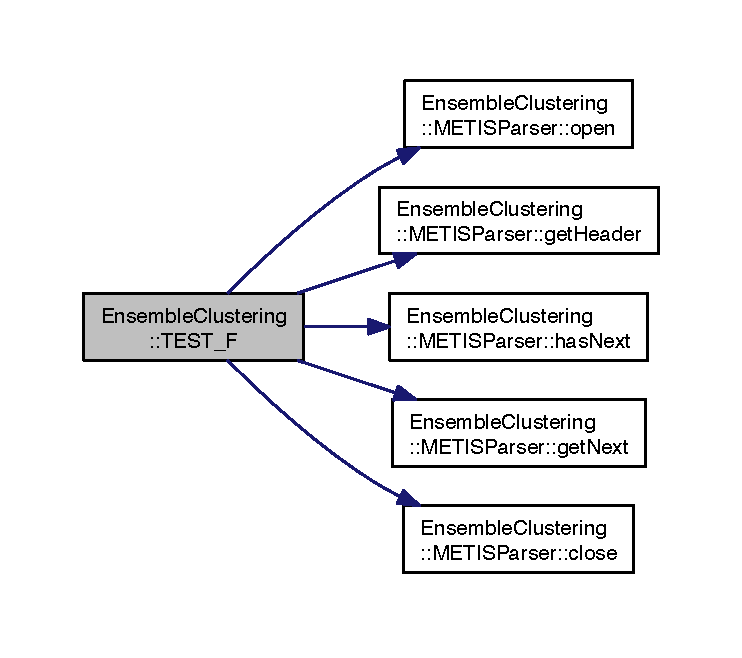
\includegraphics[width=350pt]{namespace_ensemble_clustering_a968aa929eb81f21fab68af5447226d50_cgraph}
\end{center}
\end{figure}


\hypertarget{namespace_ensemble_clustering_a21108087fb4225d2c718b2ab980a0352}{\index{Ensemble\-Clustering@{Ensemble\-Clustering}!T\-E\-S\-T\-\_\-\-F@{T\-E\-S\-T\-\_\-\-F}}
\index{T\-E\-S\-T\-\_\-\-F@{T\-E\-S\-T\-\_\-\-F}!EnsembleClustering@{Ensemble\-Clustering}}
\subsubsection[{T\-E\-S\-T\-\_\-\-F}]{\setlength{\rightskip}{0pt plus 5cm}Ensemble\-Clustering\-::\-T\-E\-S\-T\-\_\-\-F (
\begin{DoxyParamCaption}
\item[{Clustering\-Test}]{, }
\item[{test\-Modularity}]{}
\end{DoxyParamCaption}
)}}\label{namespace_ensemble_clustering_a21108087fb4225d2c718b2ab980a0352}


Definition at line 29 of file Clustering\-Test.\-h.



Here is the call graph for this function\-:
\nopagebreak
\begin{figure}[H]
\begin{center}
\leavevmode
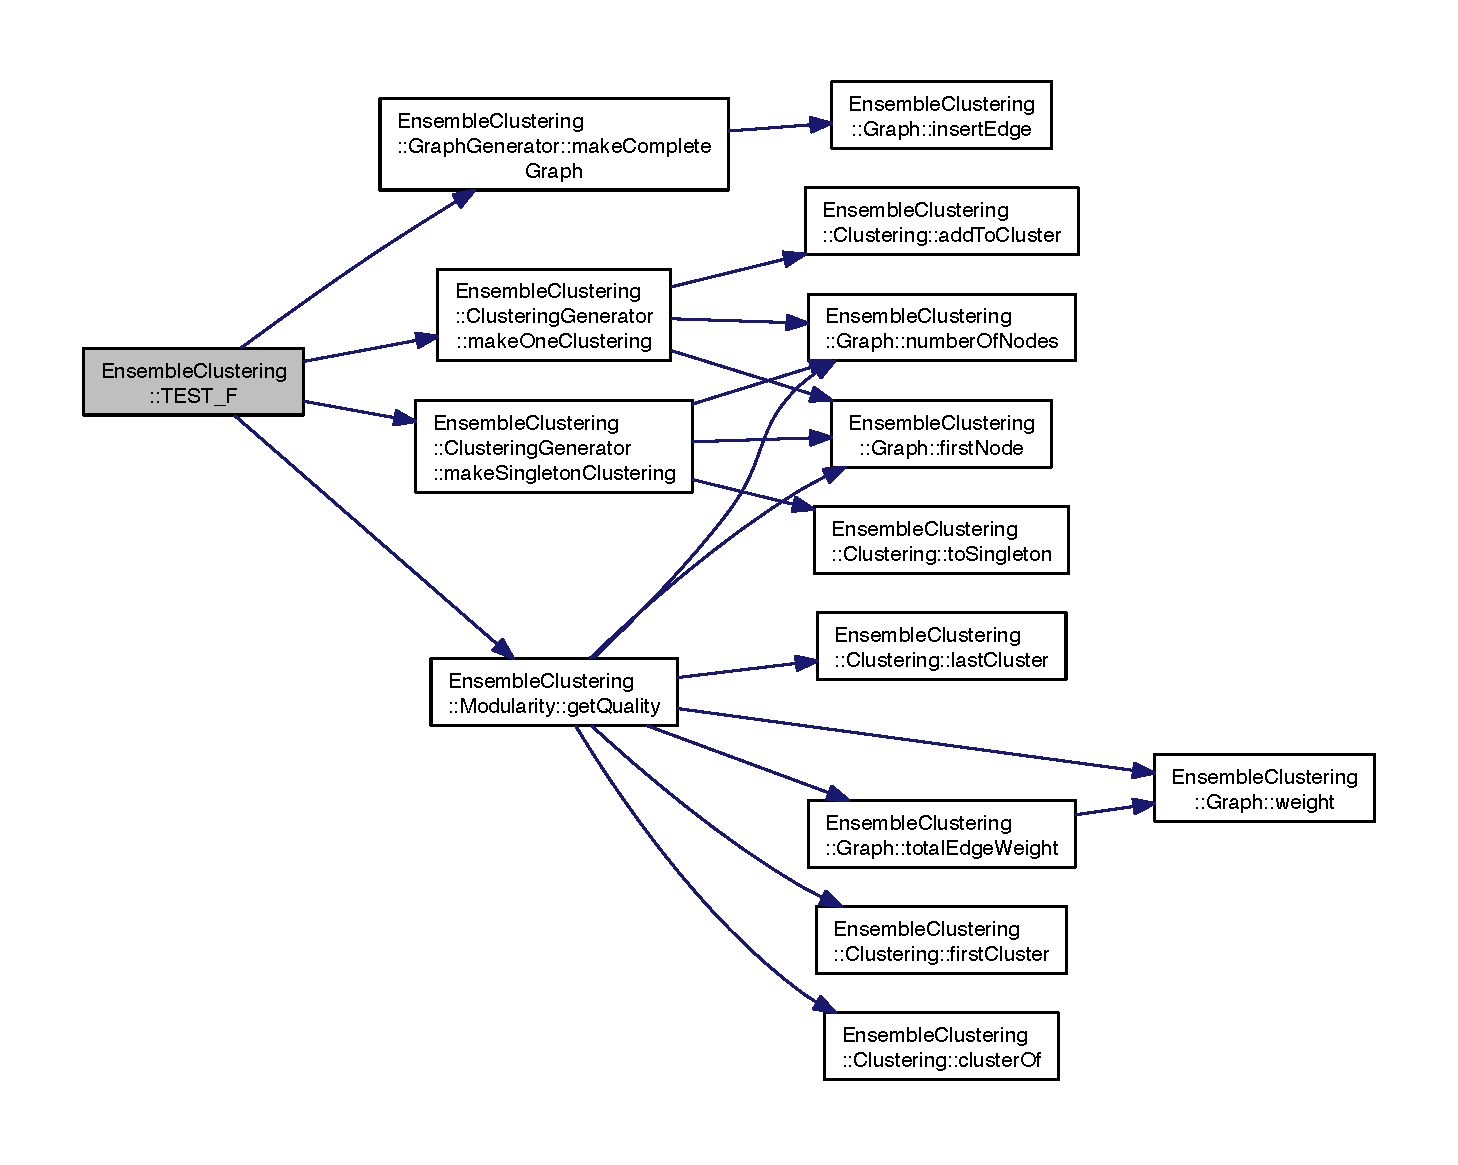
\includegraphics[width=350pt]{namespace_ensemble_clustering_a21108087fb4225d2c718b2ab980a0352_cgraph}
\end{center}
\end{figure}


\hypertarget{namespace_ensemble_clustering_ab112b02697a12bdbc3b4e866d60444d3}{\index{Ensemble\-Clustering@{Ensemble\-Clustering}!T\-E\-S\-T\-\_\-\-F@{T\-E\-S\-T\-\_\-\-F}}
\index{T\-E\-S\-T\-\_\-\-F@{T\-E\-S\-T\-\_\-\-F}!EnsembleClustering@{Ensemble\-Clustering}}
\subsubsection[{T\-E\-S\-T\-\_\-\-F}]{\setlength{\rightskip}{0pt plus 5cm}Ensemble\-Clustering\-::\-T\-E\-S\-T\-\_\-\-F (
\begin{DoxyParamCaption}
\item[{Graph\-G\-Test}]{, }
\item[{test\-Iteration}]{}
\end{DoxyParamCaption}
)}}\label{namespace_ensemble_clustering_ab112b02697a12bdbc3b4e866d60444d3}


Definition at line 34 of file Graph\-G\-Test.\-h.



Here is the call graph for this function\-:
\nopagebreak
\begin{figure}[H]
\begin{center}
\leavevmode
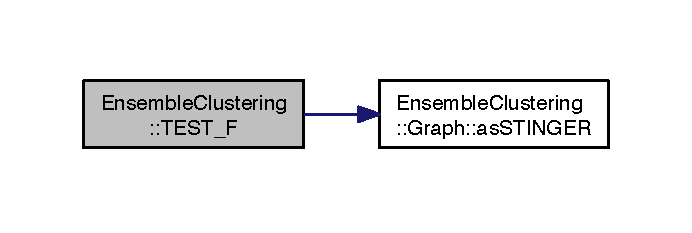
\includegraphics[width=332pt]{namespace_ensemble_clustering_ab112b02697a12bdbc3b4e866d60444d3_cgraph}
\end{center}
\end{figure}



\chapter{Class Documentation}
\hypertarget{class_ensemble_clustering_1_1_cluster_contracter}{\section{Ensemble\-Clustering\-:\-:Cluster\-Contracter Class Reference}
\label{class_ensemble_clustering_1_1_cluster_contracter}\index{Ensemble\-Clustering\-::\-Cluster\-Contracter@{Ensemble\-Clustering\-::\-Cluster\-Contracter}}
}


{\ttfamily \#include $<$Cluster\-Contracter.\-h$>$}



Inheritance diagram for Ensemble\-Clustering\-:\-:Cluster\-Contracter\-:\nopagebreak
\begin{figure}[H]
\begin{center}
\leavevmode
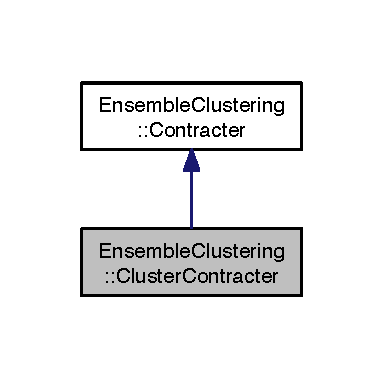
\includegraphics[width=184pt]{class_ensemble_clustering_1_1_cluster_contracter__inherit__graph}
\end{center}
\end{figure}


Collaboration diagram for Ensemble\-Clustering\-:\-:Cluster\-Contracter\-:\nopagebreak
\begin{figure}[H]
\begin{center}
\leavevmode
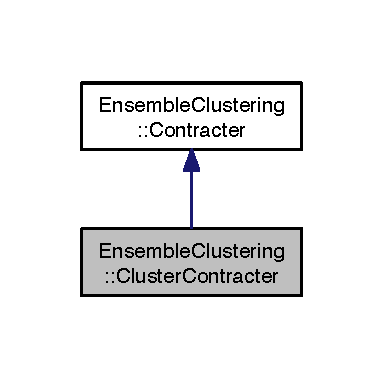
\includegraphics[width=184pt]{class_ensemble_clustering_1_1_cluster_contracter__coll__graph}
\end{center}
\end{figure}
\subsection*{Public Member Functions}
\begin{DoxyCompactItemize}
\item 
\hyperlink{class_ensemble_clustering_1_1_cluster_contracter_ac51b010f87f4c411362708db2c07ab30}{Cluster\-Contracter} ()
\item 
virtual \hyperlink{class_ensemble_clustering_1_1_cluster_contracter_ac992fc137b558a57310336fa593200e0}{$\sim$\-Cluster\-Contracter} ()
\end{DoxyCompactItemize}


\subsection{Detailed Description}


Definition at line 15 of file Cluster\-Contracter.\-h.



\subsection{Constructor \& Destructor Documentation}
\hypertarget{class_ensemble_clustering_1_1_cluster_contracter_ac51b010f87f4c411362708db2c07ab30}{\index{Ensemble\-Clustering\-::\-Cluster\-Contracter@{Ensemble\-Clustering\-::\-Cluster\-Contracter}!Cluster\-Contracter@{Cluster\-Contracter}}
\index{Cluster\-Contracter@{Cluster\-Contracter}!EnsembleClustering::ClusterContracter@{Ensemble\-Clustering\-::\-Cluster\-Contracter}}
\subsubsection[{Cluster\-Contracter}]{\setlength{\rightskip}{0pt plus 5cm}Ensemble\-Clustering\-::\-Cluster\-Contracter\-::\-Cluster\-Contracter (
\begin{DoxyParamCaption}
{}
\end{DoxyParamCaption}
)}}\label{class_ensemble_clustering_1_1_cluster_contracter_ac51b010f87f4c411362708db2c07ab30}


Definition at line 12 of file Cluster\-Contracter.\-cpp.

\hypertarget{class_ensemble_clustering_1_1_cluster_contracter_ac992fc137b558a57310336fa593200e0}{\index{Ensemble\-Clustering\-::\-Cluster\-Contracter@{Ensemble\-Clustering\-::\-Cluster\-Contracter}!$\sim$\-Cluster\-Contracter@{$\sim$\-Cluster\-Contracter}}
\index{$\sim$\-Cluster\-Contracter@{$\sim$\-Cluster\-Contracter}!EnsembleClustering::ClusterContracter@{Ensemble\-Clustering\-::\-Cluster\-Contracter}}
\subsubsection[{$\sim$\-Cluster\-Contracter}]{\setlength{\rightskip}{0pt plus 5cm}Ensemble\-Clustering\-::\-Cluster\-Contracter\-::$\sim$\-Cluster\-Contracter (
\begin{DoxyParamCaption}
{}
\end{DoxyParamCaption}
)\hspace{0.3cm}{\ttfamily [virtual]}}}\label{class_ensemble_clustering_1_1_cluster_contracter_ac992fc137b558a57310336fa593200e0}


Definition at line 17 of file Cluster\-Contracter.\-cpp.



The documentation for this class was generated from the following files\-:\begin{DoxyCompactItemize}
\item 
src/coarsening/\hyperlink{_cluster_contracter_8h}{Cluster\-Contracter.\-h}\item 
src/coarsening/\hyperlink{_cluster_contracter_8cpp}{Cluster\-Contracter.\-cpp}\end{DoxyCompactItemize}

\hypertarget{class_ensemble_clustering_1_1_clusterer}{\section{Ensemble\-Clustering\-:\-:Clusterer Class Reference}
\label{class_ensemble_clustering_1_1_clusterer}\index{Ensemble\-Clustering\-::\-Clusterer@{Ensemble\-Clustering\-::\-Clusterer}}
}


{\ttfamily \#include $<$Clusterer.\-h$>$}



Inheritance diagram for Ensemble\-Clustering\-:\-:Clusterer\-:\nopagebreak
\begin{figure}[H]
\begin{center}
\leavevmode
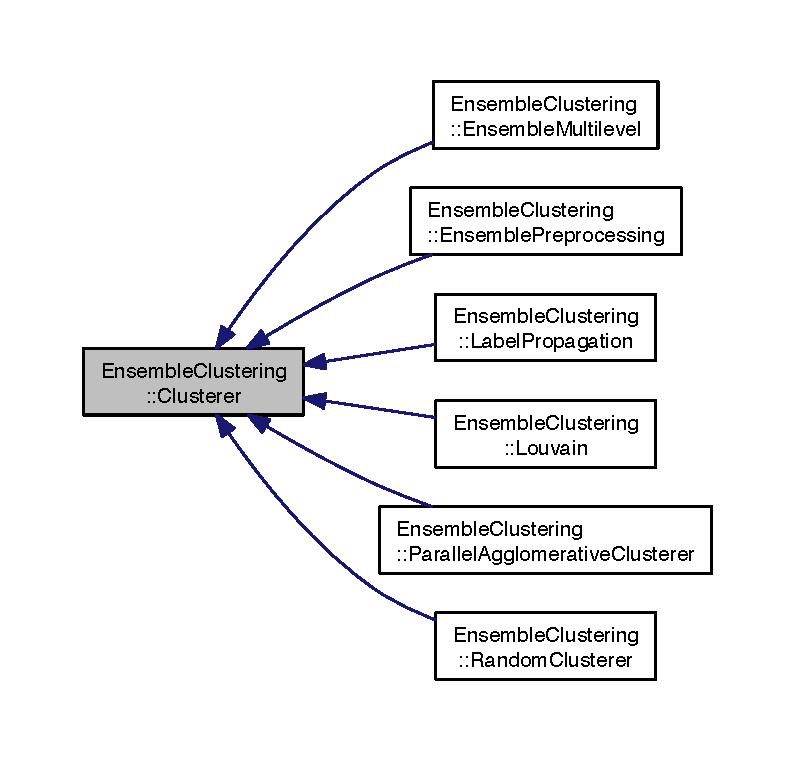
\includegraphics[width=315pt]{class_ensemble_clustering_1_1_clusterer__inherit__graph}
\end{center}
\end{figure}
\subsection*{Public Member Functions}
\begin{DoxyCompactItemize}
\item 
\hyperlink{class_ensemble_clustering_1_1_clusterer_acbd9729676a2793bccffbacec6bd13f9}{Clusterer} ()
\item 
virtual \hyperlink{class_ensemble_clustering_1_1_clusterer_a93a0ef31adf30861adc1db201174953f}{$\sim$\-Clusterer} ()
\item 
virtual \hyperlink{class_ensemble_clustering_1_1_clustering}{Clustering} \& \hyperlink{class_ensemble_clustering_1_1_clusterer_a4266e5bb967201f6567ce299bbc2f662}{run} (\hyperlink{class_ensemble_clustering_1_1_graph}{Graph} \&G)=0
\end{DoxyCompactItemize}


\subsection{Detailed Description}


Definition at line 17 of file Clusterer.\-h.



\subsection{Constructor \& Destructor Documentation}
\hypertarget{class_ensemble_clustering_1_1_clusterer_acbd9729676a2793bccffbacec6bd13f9}{\index{Ensemble\-Clustering\-::\-Clusterer@{Ensemble\-Clustering\-::\-Clusterer}!Clusterer@{Clusterer}}
\index{Clusterer@{Clusterer}!EnsembleClustering::Clusterer@{Ensemble\-Clustering\-::\-Clusterer}}
\subsubsection[{Clusterer}]{\setlength{\rightskip}{0pt plus 5cm}Ensemble\-Clustering\-::\-Clusterer\-::\-Clusterer (
\begin{DoxyParamCaption}
{}
\end{DoxyParamCaption}
)}}\label{class_ensemble_clustering_1_1_clusterer_acbd9729676a2793bccffbacec6bd13f9}


Definition at line 12 of file Clusterer.\-cpp.

\hypertarget{class_ensemble_clustering_1_1_clusterer_a93a0ef31adf30861adc1db201174953f}{\index{Ensemble\-Clustering\-::\-Clusterer@{Ensemble\-Clustering\-::\-Clusterer}!$\sim$\-Clusterer@{$\sim$\-Clusterer}}
\index{$\sim$\-Clusterer@{$\sim$\-Clusterer}!EnsembleClustering::Clusterer@{Ensemble\-Clustering\-::\-Clusterer}}
\subsubsection[{$\sim$\-Clusterer}]{\setlength{\rightskip}{0pt plus 5cm}Ensemble\-Clustering\-::\-Clusterer\-::$\sim$\-Clusterer (
\begin{DoxyParamCaption}
{}
\end{DoxyParamCaption}
)\hspace{0.3cm}{\ttfamily [virtual]}}}\label{class_ensemble_clustering_1_1_clusterer_a93a0ef31adf30861adc1db201174953f}


Definition at line 17 of file Clusterer.\-cpp.



\subsection{Member Function Documentation}
\hypertarget{class_ensemble_clustering_1_1_clusterer_a4266e5bb967201f6567ce299bbc2f662}{\index{Ensemble\-Clustering\-::\-Clusterer@{Ensemble\-Clustering\-::\-Clusterer}!run@{run}}
\index{run@{run}!EnsembleClustering::Clusterer@{Ensemble\-Clustering\-::\-Clusterer}}
\subsubsection[{run}]{\setlength{\rightskip}{0pt plus 5cm}virtual {\bf Clustering}\& Ensemble\-Clustering\-::\-Clusterer\-::run (
\begin{DoxyParamCaption}
\item[{{\bf Graph} \&}]{G}
\end{DoxyParamCaption}
)\hspace{0.3cm}{\ttfamily [pure virtual]}}}\label{class_ensemble_clustering_1_1_clusterer_a4266e5bb967201f6567ce299bbc2f662}


Implemented in \hyperlink{class_ensemble_clustering_1_1_label_propagation_a4915a00c1a2dc5a07c7d902bcb66f52a}{Ensemble\-Clustering\-::\-Label\-Propagation}.



The documentation for this class was generated from the following files\-:\begin{DoxyCompactItemize}
\item 
src/clustering/\hyperlink{_clusterer_8h}{Clusterer.\-h}\item 
src/clustering/\hyperlink{_clusterer_8cpp}{Clusterer.\-cpp}\end{DoxyCompactItemize}

\hypertarget{class_ensemble_clustering_1_1_clustering}{\section{Ensemble\-Clustering\-:\-:Clustering Class Reference}
\label{class_ensemble_clustering_1_1_clustering}\index{Ensemble\-Clustering\-::\-Clustering@{Ensemble\-Clustering\-::\-Clustering}}
}


{\ttfamily \#include $<$Clustering.\-h$>$}



Inheritance diagram for Ensemble\-Clustering\-:\-:Clustering\-:
\nopagebreak
\begin{figure}[H]
\begin{center}
\leavevmode
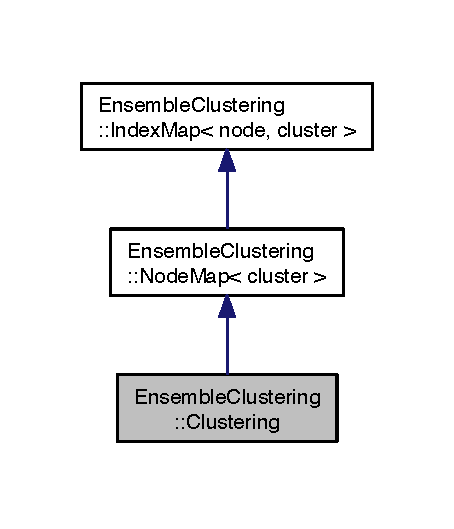
\includegraphics[width=218pt]{class_ensemble_clustering_1_1_clustering__inherit__graph}
\end{center}
\end{figure}


Collaboration diagram for Ensemble\-Clustering\-:\-:Clustering\-:
\nopagebreak
\begin{figure}[H]
\begin{center}
\leavevmode
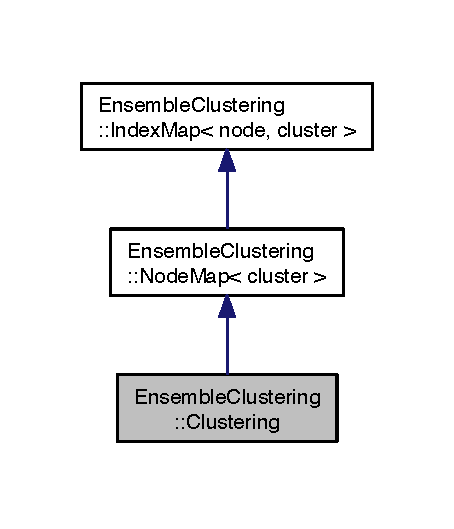
\includegraphics[width=218pt]{class_ensemble_clustering_1_1_clustering__coll__graph}
\end{center}
\end{figure}
\subsection*{Public Member Functions}
\begin{DoxyCompactItemize}
\item 
\hyperlink{class_ensemble_clustering_1_1_clustering_ad1851ed55e02294c6ed7f621d5f6e0fc}{Clustering} (\hyperlink{namespace_ensemble_clustering_a2482e94ca22a0c6544a5a9173186fde8}{count} \hyperlink{class_ensemble_clustering_1_1_index_map_a3151d302c54e6ad0175bd87aef62d4ca}{n})
\begin{DoxyCompactList}\small\item\em Construct new clustering. \end{DoxyCompactList}\item 
virtual \hyperlink{class_ensemble_clustering_1_1_clustering_ad7d81b7dc44d96c4802e1294e3ffbb48}{$\sim$\-Clustering} ()
\item 
void \hyperlink{class_ensemble_clustering_1_1_clustering_a983184e9efa473931ae7dfc9c566e666}{set\-Name} (std\-::string \hyperlink{class_ensemble_clustering_1_1_clustering_affe0177a3d80ddd03d475307a74b3a1c}{name})
\begin{DoxyCompactList}\small\item\em Set a human-\/readable identifier (vulg. \end{DoxyCompactList}\item 
std\-::string \hyperlink{class_ensemble_clustering_1_1_clustering_aaabfd9762ba3381d95e6d2bdcd95c9a9}{get\-Name} () const 
\begin{DoxyCompactList}\small\item\em Get the human-\/readable identifier (vulg. \end{DoxyCompactList}\item 
\hyperlink{namespace_ensemble_clustering_a5ae38234e207add524443be6e597b970}{cluster} \& \hyperlink{class_ensemble_clustering_1_1_clustering_aaa9d16c93e56a4ea1c6bcf7eb302610a}{operator\mbox{[}$\,$\mbox{]}} (const \hyperlink{namespace_ensemble_clustering_ae829290aeccd1a420b17a37fd901f114}{node} \&u)
\begin{DoxyCompactList}\small\item\em Index operator. \end{DoxyCompactList}\item 
const \hyperlink{namespace_ensemble_clustering_a5ae38234e207add524443be6e597b970}{cluster} \& \hyperlink{class_ensemble_clustering_1_1_clustering_aa277d9365e79e8b2f067e8630a29b031}{operator\mbox{[}$\,$\mbox{]}} (const \hyperlink{namespace_ensemble_clustering_ae829290aeccd1a420b17a37fd901f114}{node} \&u) const 
\begin{DoxyCompactList}\small\item\em Index operator for const instances of this class. \end{DoxyCompactList}\item 
\hyperlink{namespace_ensemble_clustering_a5ae38234e207add524443be6e597b970}{cluster} \hyperlink{class_ensemble_clustering_1_1_clustering_a5c02c6c1b31e8517f713b978d0c079ea}{cluster\-Of} (\hyperlink{namespace_ensemble_clustering_ae829290aeccd1a420b17a37fd901f114}{node} u) const 
\begin{DoxyCompactList}\small\item\em Return the cluster (id) in which a node is contained. \end{DoxyCompactList}\item 
\hyperlink{namespace_ensemble_clustering_a5ae38234e207add524443be6e597b970}{cluster} \hyperlink{class_ensemble_clustering_1_1_clustering_af6a1379873404b3408d513026005f921}{add\-Cluster} ()
\begin{DoxyCompactList}\small\item\em Call this before assigning nodes to cluster ids. \end{DoxyCompactList}\item 
void \hyperlink{class_ensemble_clustering_1_1_clustering_a2f6334480e3938deae8425dc57e6ea86}{add\-To\-Cluster} (\hyperlink{namespace_ensemble_clustering_a5ae38234e207add524443be6e597b970}{cluster} c, \hyperlink{namespace_ensemble_clustering_ae829290aeccd1a420b17a37fd901f114}{node} u)
\begin{DoxyCompactList}\small\item\em Add a (previously unassigned) node to a cluster. \end{DoxyCompactList}\item 
void \hyperlink{class_ensemble_clustering_1_1_clustering_a7e3a719ed9904897617a3152bf80a634}{move\-To\-Cluster} (\hyperlink{namespace_ensemble_clustering_a5ae38234e207add524443be6e597b970}{cluster} c, \hyperlink{namespace_ensemble_clustering_ae829290aeccd1a420b17a37fd901f114}{node} u)
\begin{DoxyCompactList}\small\item\em Move a (previously assigned) node to a cluster. \end{DoxyCompactList}\item 
void \hyperlink{class_ensemble_clustering_1_1_clustering_a461a251d674b64cf29e97408c343253a}{to\-Singleton} (\hyperlink{namespace_ensemble_clustering_ae829290aeccd1a420b17a37fd901f114}{node} u)
\begin{DoxyCompactList}\small\item\em Creates a singleton cluster containing the node. \end{DoxyCompactList}\item 
void \hyperlink{class_ensemble_clustering_1_1_clustering_aa93abafed46c4707dac3ca4b0d445f79}{all\-To\-Singletons} ()
\begin{DoxyCompactList}\small\item\em Assigns every node to a singleton cluster. \end{DoxyCompactList}\item 
void \hyperlink{class_ensemble_clustering_1_1_clustering_a1cfe6fb096bef4aeb7814877847e2df9}{merge\-Clusters} (\hyperlink{namespace_ensemble_clustering_a5ae38234e207add524443be6e597b970}{cluster} c, \hyperlink{namespace_ensemble_clustering_a5ae38234e207add524443be6e597b970}{cluster} d)
\begin{DoxyCompactList}\small\item\em Assigns the nodes from both clusters to a new cluster. \end{DoxyCompactList}\item 
bool \hyperlink{class_ensemble_clustering_1_1_clustering_a6ef2d3f0c4a53532067a140caa531449}{is\-Proper} (\hyperlink{class_ensemble_clustering_1_1_graph}{Graph} \&G)
\begin{DoxyCompactList}\small\item\em Check whether this clustering is a proper clustering of the graph, i.\-e. \end{DoxyCompactList}\item 
bool \hyperlink{class_ensemble_clustering_1_1_clustering_ae00d7d11885b34c03969e213ec189a75}{is\-One\-Clustering} (\hyperlink{class_ensemble_clustering_1_1_graph}{Graph} \&G)
\begin{DoxyCompactList}\small\item\em Check if clustering is a 1-\/clustering, i.\-e. \end{DoxyCompactList}\item 
bool \hyperlink{class_ensemble_clustering_1_1_clustering_a49da98ece8e5e62638009ddf2cfa3929}{is\-Singleton\-Clustering} (\hyperlink{class_ensemble_clustering_1_1_graph}{Graph} \&G)
\begin{DoxyCompactList}\small\item\em Check if clustering is a singleton clustering, i.\-e. \end{DoxyCompactList}\item 
\hyperlink{namespace_ensemble_clustering_a2482e94ca22a0c6544a5a9173186fde8}{count} \hyperlink{class_ensemble_clustering_1_1_clustering_a7eb03661a933eff8176af0e073da2ef4}{number\-Of\-Clusters} () const 
\begin{DoxyCompactList}\small\item\em Get the current number of clusters in this clustering. \end{DoxyCompactList}\item 
\hyperlink{namespace_ensemble_clustering_a5ae38234e207add524443be6e597b970}{cluster} \hyperlink{class_ensemble_clustering_1_1_clustering_ae0b22bda843f96f9428d05aa582cfe4b}{upper\-Bound} () const 
\begin{DoxyCompactList}\small\item\em Return an upper bound for the cluster ids that have been assigned. \end{DoxyCompactList}\item 
\hyperlink{namespace_ensemble_clustering_a5ae38234e207add524443be6e597b970}{cluster} \hyperlink{class_ensemble_clustering_1_1_clustering_ab64cf7248533ea358d7621ca8296b085}{lower\-Bound} () const 
\begin{DoxyCompactList}\small\item\em Return a lower bound for the cluster ids that have been assigned. \end{DoxyCompactList}\item 
void \hyperlink{class_ensemble_clustering_1_1_clustering_adb704c4cbb2205b7858ac2d7f0f5014f}{set\-Upper\-Bound} (\hyperlink{namespace_ensemble_clustering_a5ae38234e207add524443be6e597b970}{cluster} id)
\begin{DoxyCompactList}\small\item\em Set an upper bound for the cluster ids. \end{DoxyCompactList}\item 
void \hyperlink{class_ensemble_clustering_1_1_clustering_a51a9ed79e7d14cd1739be0034b35e835}{compact} ()
\begin{DoxyCompactList}\small\item\em Change cluster I\-Ds to be consecutive, starting at 0. \end{DoxyCompactList}\item 
bool \hyperlink{class_ensemble_clustering_1_1_clustering_a53f22ed7ab2a41979f5cdf9b99b5e1de}{contains} (\hyperlink{namespace_ensemble_clustering_ae829290aeccd1a420b17a37fd901f114}{node} v)
\begin{DoxyCompactList}\small\item\em Check if clustering assigns a valid cluster to the node. \end{DoxyCompactList}\item 
bool \hyperlink{class_ensemble_clustering_1_1_clustering_a16c268a2020e4d8f6766d44556697e1d}{in\-Same\-Cluster} (\hyperlink{namespace_ensemble_clustering_ae829290aeccd1a420b17a37fd901f114}{node} u, \hyperlink{namespace_ensemble_clustering_ae829290aeccd1a420b17a37fd901f114}{node} v)
\begin{DoxyCompactList}\small\item\em Check if two nodes belong to the same cluster. \end{DoxyCompactList}\item 
bool \hyperlink{class_ensemble_clustering_1_1_clustering_a1ae12fcdc2549a6826ced64675a56e80}{equals} (\hyperlink{class_ensemble_clustering_1_1_clustering}{Clustering} \&other, \hyperlink{class_ensemble_clustering_1_1_graph}{Graph} \&G)
\begin{DoxyCompactList}\small\item\em E\-: (u) = (v)  (u) = (v)  (u)  (v)  (u)  (v) \$\$ \end{DoxyCompactList}\item 
{\footnotesize template$<$typename Callback $>$ }\\void \hyperlink{class_ensemble_clustering_1_1_clustering_ac73ad4ef868aa0b851f768f1a74186b7}{for\-Entries} (Callback func, std\-::string par=\char`\"{}\char`\"{})
\begin{DoxyCompactList}\small\item\em Iterate over all entries (node, cluster) and execute callback function (lambda closure). \end{DoxyCompactList}\item 
{\footnotesize template$<$typename Callback $>$ }\\void \hyperlink{class_ensemble_clustering_1_1_clustering_ace9debc0ddc3de9f505ab33f9490c7c6}{parallel\-For\-Entries} (Callback handle)
\begin{DoxyCompactList}\small\item\em Iterate over all entries (node, cluster) in parallel and execute callback function (lambda closure). \end{DoxyCompactList}\item 
std\-::vector$<$ \hyperlink{namespace_ensemble_clustering_a2482e94ca22a0c6544a5a9173186fde8}{count} $>$ \hyperlink{class_ensemble_clustering_1_1_clustering_aecf64e29e7032bdcac3f90fa76df2b0b}{cluster\-Sizes} ()
\end{DoxyCompactItemize}
\subsection*{Protected Member Functions}
\begin{DoxyCompactItemize}
\item 
\hyperlink{namespace_ensemble_clustering_a5ae38234e207add524443be6e597b970}{cluster} \hyperlink{class_ensemble_clustering_1_1_clustering_a7ab76ffd8b0068e049f854e07e8902eb}{get\-Next\-Cluster} ()
\item 
bool \hyperlink{class_ensemble_clustering_1_1_clustering_a7d8cd0be7f1bde9e7cdf2cf10c54c121}{is\-In\-Range} (\hyperlink{namespace_ensemble_clustering_ae829290aeccd1a420b17a37fd901f114}{node} v)
\begin{DoxyCompactList}\small\item\em Check if clustering can hold a valid entry for the node because it is in the range mapped. \end{DoxyCompactList}\end{DoxyCompactItemize}
\subsection*{Protected Attributes}
\begin{DoxyCompactItemize}
\item 
\hyperlink{namespace_ensemble_clustering_a5ae38234e207add524443be6e597b970}{cluster} \hyperlink{class_ensemble_clustering_1_1_clustering_a47de59cf22e93a801cac55eb001b6d3d}{next\-Cluster}
\begin{DoxyCompactList}\small\item\em next free cluster id for new cluster \end{DoxyCompactList}\item 
std\-::string \hyperlink{class_ensemble_clustering_1_1_clustering_affe0177a3d80ddd03d475307a74b3a1c}{name}
\item 
\hyperlink{namespace_ensemble_clustering_a5ae38234e207add524443be6e597b970}{cluster} \hyperlink{class_ensemble_clustering_1_1_clustering_a59e76a2bdf80c98186938c46814b9e36}{upper\-Id\-Bound}
\begin{DoxyCompactList}\small\item\em upper bound for cluster ids \end{DoxyCompactList}\end{DoxyCompactItemize}


\subsection{Detailed Description}


Definition at line 22 of file Clustering.\-h.



\subsection{Constructor \& Destructor Documentation}
\hypertarget{class_ensemble_clustering_1_1_clustering_ad1851ed55e02294c6ed7f621d5f6e0fc}{\index{Ensemble\-Clustering\-::\-Clustering@{Ensemble\-Clustering\-::\-Clustering}!Clustering@{Clustering}}
\index{Clustering@{Clustering}!EnsembleClustering::Clustering@{Ensemble\-Clustering\-::\-Clustering}}
\subsubsection[{Clustering}]{\setlength{\rightskip}{0pt plus 5cm}Ensemble\-Clustering\-::\-Clustering\-::\-Clustering (
\begin{DoxyParamCaption}
\item[{{\bf count}}]{n}
\end{DoxyParamCaption}
)}}\label{class_ensemble_clustering_1_1_clustering_ad1851ed55e02294c6ed7f621d5f6e0fc}


Construct new clustering. 


\begin{DoxyParams}[1]{Parameters}
\mbox{\tt in}  & {\em n} & number of nodes \\
\hline
\end{DoxyParams}


Definition at line 13 of file Clustering.\-cpp.

\hypertarget{class_ensemble_clustering_1_1_clustering_ad7d81b7dc44d96c4802e1294e3ffbb48}{\index{Ensemble\-Clustering\-::\-Clustering@{Ensemble\-Clustering\-::\-Clustering}!$\sim$\-Clustering@{$\sim$\-Clustering}}
\index{$\sim$\-Clustering@{$\sim$\-Clustering}!EnsembleClustering::Clustering@{Ensemble\-Clustering\-::\-Clustering}}
\subsubsection[{$\sim$\-Clustering}]{\setlength{\rightskip}{0pt plus 5cm}Ensemble\-Clustering\-::\-Clustering\-::$\sim$\-Clustering (
\begin{DoxyParamCaption}
{}
\end{DoxyParamCaption}
)\hspace{0.3cm}{\ttfamily [virtual]}}}\label{class_ensemble_clustering_1_1_clustering_ad7d81b7dc44d96c4802e1294e3ffbb48}


Definition at line 20 of file Clustering.\-cpp.



\subsection{Member Function Documentation}
\hypertarget{class_ensemble_clustering_1_1_clustering_af6a1379873404b3408d513026005f921}{\index{Ensemble\-Clustering\-::\-Clustering@{Ensemble\-Clustering\-::\-Clustering}!add\-Cluster@{add\-Cluster}}
\index{add\-Cluster@{add\-Cluster}!EnsembleClustering::Clustering@{Ensemble\-Clustering\-::\-Clustering}}
\subsubsection[{add\-Cluster}]{\setlength{\rightskip}{0pt plus 5cm}{\bf cluster} Ensemble\-Clustering\-::\-Clustering\-::add\-Cluster (
\begin{DoxyParamCaption}
{}
\end{DoxyParamCaption}
)}}\label{class_ensemble_clustering_1_1_clustering_af6a1379873404b3408d513026005f921}


Call this before assigning nodes to cluster ids. 



Definition at line 87 of file Clustering.\-cpp.

\hypertarget{class_ensemble_clustering_1_1_clustering_a2f6334480e3938deae8425dc57e6ea86}{\index{Ensemble\-Clustering\-::\-Clustering@{Ensemble\-Clustering\-::\-Clustering}!add\-To\-Cluster@{add\-To\-Cluster}}
\index{add\-To\-Cluster@{add\-To\-Cluster}!EnsembleClustering::Clustering@{Ensemble\-Clustering\-::\-Clustering}}
\subsubsection[{add\-To\-Cluster}]{\setlength{\rightskip}{0pt plus 5cm}void Ensemble\-Clustering\-::\-Clustering\-::add\-To\-Cluster (
\begin{DoxyParamCaption}
\item[{{\bf cluster}}]{c, }
\item[{{\bf node}}]{u}
\end{DoxyParamCaption}
)}}\label{class_ensemble_clustering_1_1_clustering_a2f6334480e3938deae8425dc57e6ea86}


Add a (previously unassigned) node to a cluster. 



Definition at line 24 of file Clustering.\-cpp.

\hypertarget{class_ensemble_clustering_1_1_clustering_aa93abafed46c4707dac3ca4b0d445f79}{\index{Ensemble\-Clustering\-::\-Clustering@{Ensemble\-Clustering\-::\-Clustering}!all\-To\-Singletons@{all\-To\-Singletons}}
\index{all\-To\-Singletons@{all\-To\-Singletons}!EnsembleClustering::Clustering@{Ensemble\-Clustering\-::\-Clustering}}
\subsubsection[{all\-To\-Singletons}]{\setlength{\rightskip}{0pt plus 5cm}void Ensemble\-Clustering\-::\-Clustering\-::all\-To\-Singletons (
\begin{DoxyParamCaption}
{}
\end{DoxyParamCaption}
)}}\label{class_ensemble_clustering_1_1_clustering_aa93abafed46c4707dac3ca4b0d445f79}


Assigns every node to a singleton cluster. 

Cluster id is equal to node id. 

Definition at line 80 of file Clustering.\-cpp.

\hypertarget{class_ensemble_clustering_1_1_clustering_a5c02c6c1b31e8517f713b978d0c079ea}{\index{Ensemble\-Clustering\-::\-Clustering@{Ensemble\-Clustering\-::\-Clustering}!cluster\-Of@{cluster\-Of}}
\index{cluster\-Of@{cluster\-Of}!EnsembleClustering::Clustering@{Ensemble\-Clustering\-::\-Clustering}}
\subsubsection[{cluster\-Of}]{\setlength{\rightskip}{0pt plus 5cm}{\bf cluster} Ensemble\-Clustering\-::\-Clustering\-::cluster\-Of (
\begin{DoxyParamCaption}
\item[{{\bf node}}]{u}
\end{DoxyParamCaption}
) const\hspace{0.3cm}{\ttfamily [inline]}}}\label{class_ensemble_clustering_1_1_clustering_a5c02c6c1b31e8517f713b978d0c079ea}


Return the cluster (id) in which a node is contained. 



Definition at line 87 of file Clustering.\-h.



Here is the call graph for this function\-:
\nopagebreak
\begin{figure}[H]
\begin{center}
\leavevmode
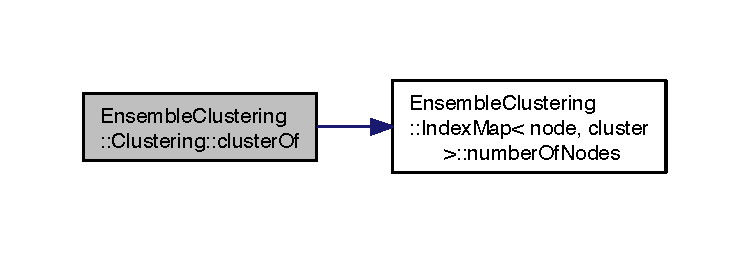
\includegraphics[width=350pt]{class_ensemble_clustering_1_1_clustering_a5c02c6c1b31e8517f713b978d0c079ea_cgraph}
\end{center}
\end{figure}


\hypertarget{class_ensemble_clustering_1_1_clustering_aecf64e29e7032bdcac3f90fa76df2b0b}{\index{Ensemble\-Clustering\-::\-Clustering@{Ensemble\-Clustering\-::\-Clustering}!cluster\-Sizes@{cluster\-Sizes}}
\index{cluster\-Sizes@{cluster\-Sizes}!EnsembleClustering::Clustering@{Ensemble\-Clustering\-::\-Clustering}}
\subsubsection[{cluster\-Sizes}]{\setlength{\rightskip}{0pt plus 5cm}std\-::vector$<$ {\bf count} $>$ Ensemble\-Clustering\-::\-Clustering\-::cluster\-Sizes (
\begin{DoxyParamCaption}
{}
\end{DoxyParamCaption}
)}}\label{class_ensemble_clustering_1_1_clustering_aecf64e29e7032bdcac3f90fa76df2b0b}


Definition at line 169 of file Clustering.\-cpp.



Here is the call graph for this function\-:
\nopagebreak
\begin{figure}[H]
\begin{center}
\leavevmode
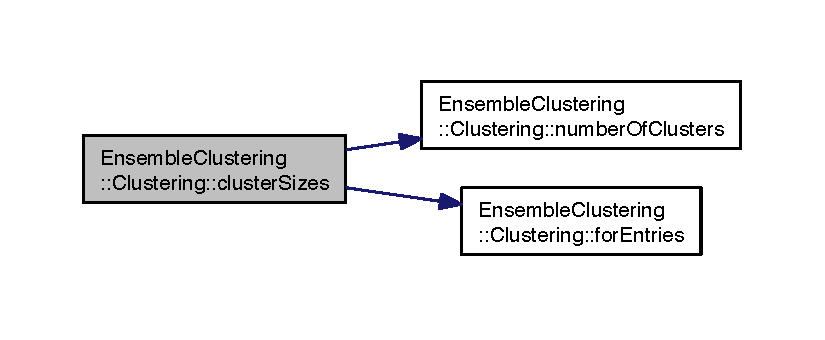
\includegraphics[width=350pt]{class_ensemble_clustering_1_1_clustering_aecf64e29e7032bdcac3f90fa76df2b0b_cgraph}
\end{center}
\end{figure}


\hypertarget{class_ensemble_clustering_1_1_clustering_a51a9ed79e7d14cd1739be0034b35e835}{\index{Ensemble\-Clustering\-::\-Clustering@{Ensemble\-Clustering\-::\-Clustering}!compact@{compact}}
\index{compact@{compact}!EnsembleClustering::Clustering@{Ensemble\-Clustering\-::\-Clustering}}
\subsubsection[{compact}]{\setlength{\rightskip}{0pt plus 5cm}void Ensemble\-Clustering\-::\-Clustering\-::compact (
\begin{DoxyParamCaption}
{}
\end{DoxyParamCaption}
)}}\label{class_ensemble_clustering_1_1_clustering_a51a9ed79e7d14cd1739be0034b35e835}


Change cluster I\-Ds to be consecutive, starting at 0. 



Definition at line 147 of file Clustering.\-cpp.



Here is the call graph for this function\-:
\nopagebreak
\begin{figure}[H]
\begin{center}
\leavevmode
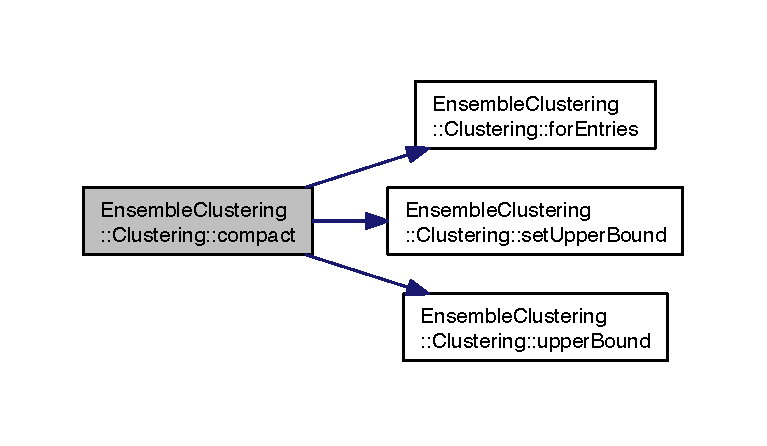
\includegraphics[width=350pt]{class_ensemble_clustering_1_1_clustering_a51a9ed79e7d14cd1739be0034b35e835_cgraph}
\end{center}
\end{figure}


\hypertarget{class_ensemble_clustering_1_1_clustering_a53f22ed7ab2a41979f5cdf9b99b5e1de}{\index{Ensemble\-Clustering\-::\-Clustering@{Ensemble\-Clustering\-::\-Clustering}!contains@{contains}}
\index{contains@{contains}!EnsembleClustering::Clustering@{Ensemble\-Clustering\-::\-Clustering}}
\subsubsection[{contains}]{\setlength{\rightskip}{0pt plus 5cm}bool Ensemble\-Clustering\-::\-Clustering\-::contains (
\begin{DoxyParamCaption}
\item[{{\bf node}}]{v}
\end{DoxyParamCaption}
)}}\label{class_ensemble_clustering_1_1_clustering_a53f22ed7ab2a41979f5cdf9b99b5e1de}


Check if clustering assigns a valid cluster to the node. 



Definition at line 97 of file Clustering.\-cpp.

\hypertarget{class_ensemble_clustering_1_1_clustering_a1ae12fcdc2549a6826ced64675a56e80}{\index{Ensemble\-Clustering\-::\-Clustering@{Ensemble\-Clustering\-::\-Clustering}!equals@{equals}}
\index{equals@{equals}!EnsembleClustering::Clustering@{Ensemble\-Clustering\-::\-Clustering}}
\subsubsection[{equals}]{\setlength{\rightskip}{0pt plus 5cm}bool Ensemble\-Clustering\-::\-Clustering\-::equals (
\begin{DoxyParamCaption}
\item[{{\bf Clustering} \&}]{other, }
\item[{{\bf Graph} \&}]{G}
\end{DoxyParamCaption}
)}}\label{class_ensemble_clustering_1_1_clustering_a1ae12fcdc2549a6826ced64675a56e80}


E\-: (u) = (v)  (u) = (v)  (u)  (v)  (u)  (v) \$\$ 



Definition at line 124 of file Clustering.\-cpp.



Here is the call graph for this function\-:
\nopagebreak
\begin{figure}[H]
\begin{center}
\leavevmode
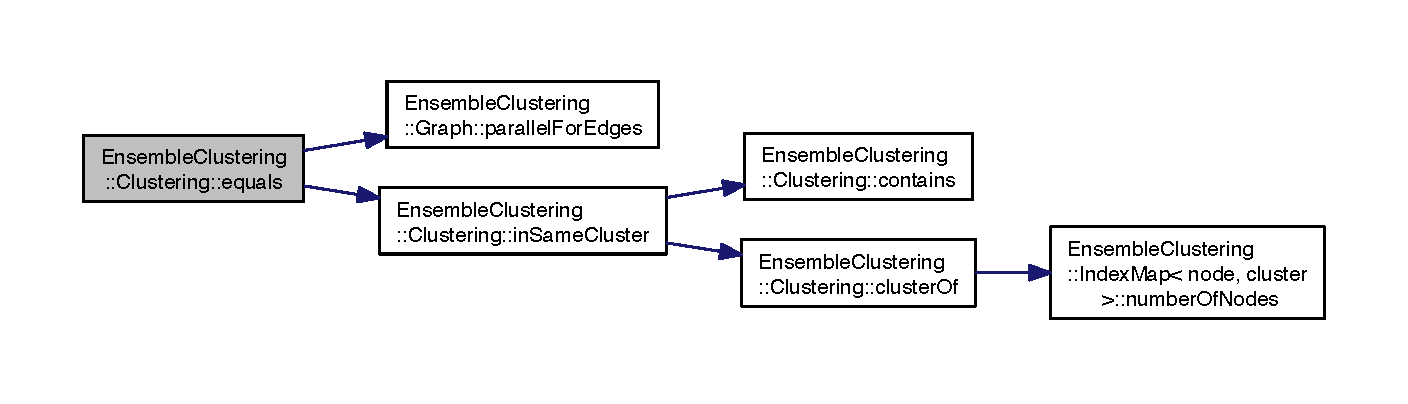
\includegraphics[width=350pt]{class_ensemble_clustering_1_1_clustering_a1ae12fcdc2549a6826ced64675a56e80_cgraph}
\end{center}
\end{figure}


\hypertarget{class_ensemble_clustering_1_1_clustering_ac73ad4ef868aa0b851f768f1a74186b7}{\index{Ensemble\-Clustering\-::\-Clustering@{Ensemble\-Clustering\-::\-Clustering}!for\-Entries@{for\-Entries}}
\index{for\-Entries@{for\-Entries}!EnsembleClustering::Clustering@{Ensemble\-Clustering\-::\-Clustering}}
\subsubsection[{for\-Entries}]{\setlength{\rightskip}{0pt plus 5cm}template$<$typename Callback $>$ void Ensemble\-Clustering\-::\-Clustering\-::for\-Entries (
\begin{DoxyParamCaption}
\item[{Callback}]{func, }
\item[{std\-::string}]{par = {\ttfamily \char`\"{}\char`\"{}}}
\end{DoxyParamCaption}
)\hspace{0.3cm}{\ttfamily [inline]}}}\label{class_ensemble_clustering_1_1_clustering_ac73ad4ef868aa0b851f768f1a74186b7}


Iterate over all entries (node, cluster) and execute callback function (lambda closure). 



Definition at line 222 of file Clustering.\-h.

\hypertarget{class_ensemble_clustering_1_1_clustering_aaabfd9762ba3381d95e6d2bdcd95c9a9}{\index{Ensemble\-Clustering\-::\-Clustering@{Ensemble\-Clustering\-::\-Clustering}!get\-Name@{get\-Name}}
\index{get\-Name@{get\-Name}!EnsembleClustering::Clustering@{Ensemble\-Clustering\-::\-Clustering}}
\subsubsection[{get\-Name}]{\setlength{\rightskip}{0pt plus 5cm}std\-::string Ensemble\-Clustering\-::\-Clustering\-::get\-Name (
\begin{DoxyParamCaption}
{}
\end{DoxyParamCaption}
) const}}\label{class_ensemble_clustering_1_1_clustering_aaabfd9762ba3381d95e6d2bdcd95c9a9}


Get the human-\/readable identifier (vulg. 

the \char`\"{}name\char`\"{}) of the graph 

Definition at line 106 of file Clustering.\-cpp.

\hypertarget{class_ensemble_clustering_1_1_clustering_a7ab76ffd8b0068e049f854e07e8902eb}{\index{Ensemble\-Clustering\-::\-Clustering@{Ensemble\-Clustering\-::\-Clustering}!get\-Next\-Cluster@{get\-Next\-Cluster}}
\index{get\-Next\-Cluster@{get\-Next\-Cluster}!EnsembleClustering::Clustering@{Ensemble\-Clustering\-::\-Clustering}}
\subsubsection[{get\-Next\-Cluster}]{\setlength{\rightskip}{0pt plus 5cm}{\bf cluster} Ensemble\-Clustering\-::\-Clustering\-::get\-Next\-Cluster (
\begin{DoxyParamCaption}
{}
\end{DoxyParamCaption}
)\hspace{0.3cm}{\ttfamily [inline]}, {\ttfamily [protected]}}}\label{class_ensemble_clustering_1_1_clustering_a7ab76ffd8b0068e049f854e07e8902eb}


Definition at line 30 of file Clustering.\-h.

\hypertarget{class_ensemble_clustering_1_1_clustering_a16c268a2020e4d8f6766d44556697e1d}{\index{Ensemble\-Clustering\-::\-Clustering@{Ensemble\-Clustering\-::\-Clustering}!in\-Same\-Cluster@{in\-Same\-Cluster}}
\index{in\-Same\-Cluster@{in\-Same\-Cluster}!EnsembleClustering::Clustering@{Ensemble\-Clustering\-::\-Clustering}}
\subsubsection[{in\-Same\-Cluster}]{\setlength{\rightskip}{0pt plus 5cm}bool Ensemble\-Clustering\-::\-Clustering\-::in\-Same\-Cluster (
\begin{DoxyParamCaption}
\item[{{\bf node}}]{u, }
\item[{{\bf node}}]{v}
\end{DoxyParamCaption}
)}}\label{class_ensemble_clustering_1_1_clustering_a16c268a2020e4d8f6766d44556697e1d}


Check if two nodes belong to the same cluster. 



Definition at line 118 of file Clustering.\-cpp.



Here is the call graph for this function\-:
\nopagebreak
\begin{figure}[H]
\begin{center}
\leavevmode
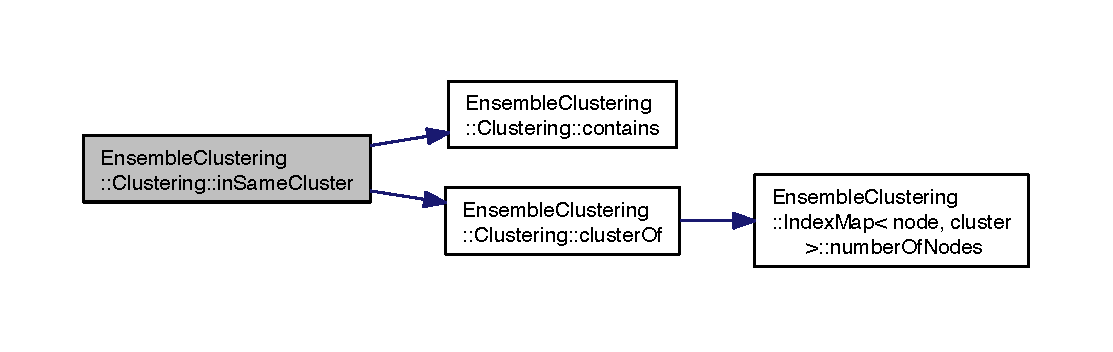
\includegraphics[width=350pt]{class_ensemble_clustering_1_1_clustering_a16c268a2020e4d8f6766d44556697e1d_cgraph}
\end{center}
\end{figure}


\hypertarget{class_ensemble_clustering_1_1_clustering_a7d8cd0be7f1bde9e7cdf2cf10c54c121}{\index{Ensemble\-Clustering\-::\-Clustering@{Ensemble\-Clustering\-::\-Clustering}!is\-In\-Range@{is\-In\-Range}}
\index{is\-In\-Range@{is\-In\-Range}!EnsembleClustering::Clustering@{Ensemble\-Clustering\-::\-Clustering}}
\subsubsection[{is\-In\-Range}]{\setlength{\rightskip}{0pt plus 5cm}bool Ensemble\-Clustering\-::\-Clustering\-::is\-In\-Range (
\begin{DoxyParamCaption}
\item[{{\bf node}}]{v}
\end{DoxyParamCaption}
)\hspace{0.3cm}{\ttfamily [protected]}}}\label{class_ensemble_clustering_1_1_clustering_a7d8cd0be7f1bde9e7cdf2cf10c54c121}


Check if clustering can hold a valid entry for the node because it is in the range mapped. 



Definition at line 93 of file Clustering.\-cpp.



Here is the call graph for this function\-:
\nopagebreak
\begin{figure}[H]
\begin{center}
\leavevmode
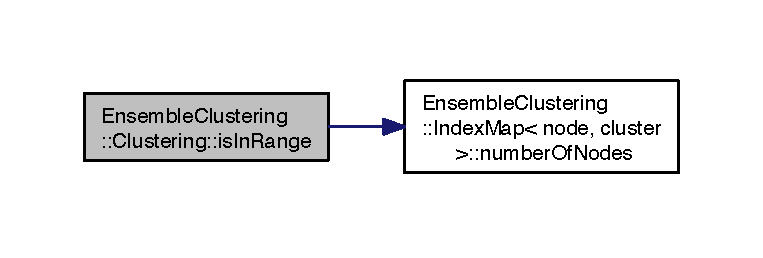
\includegraphics[width=350pt]{class_ensemble_clustering_1_1_clustering_a7d8cd0be7f1bde9e7cdf2cf10c54c121_cgraph}
\end{center}
\end{figure}


\hypertarget{class_ensemble_clustering_1_1_clustering_ae00d7d11885b34c03969e213ec189a75}{\index{Ensemble\-Clustering\-::\-Clustering@{Ensemble\-Clustering\-::\-Clustering}!is\-One\-Clustering@{is\-One\-Clustering}}
\index{is\-One\-Clustering@{is\-One\-Clustering}!EnsembleClustering::Clustering@{Ensemble\-Clustering\-::\-Clustering}}
\subsubsection[{is\-One\-Clustering}]{\setlength{\rightskip}{0pt plus 5cm}bool Ensemble\-Clustering\-::\-Clustering\-::is\-One\-Clustering (
\begin{DoxyParamCaption}
\item[{{\bf Graph} \&}]{G}
\end{DoxyParamCaption}
)}}\label{class_ensemble_clustering_1_1_clustering_ae00d7d11885b34c03969e213ec189a75}


Check if clustering is a 1-\/clustering, i.\-e. 

every node is assigned to the same cluster. 

Definition at line 110 of file Clustering.\-cpp.



Here is the call graph for this function\-:
\nopagebreak
\begin{figure}[H]
\begin{center}
\leavevmode
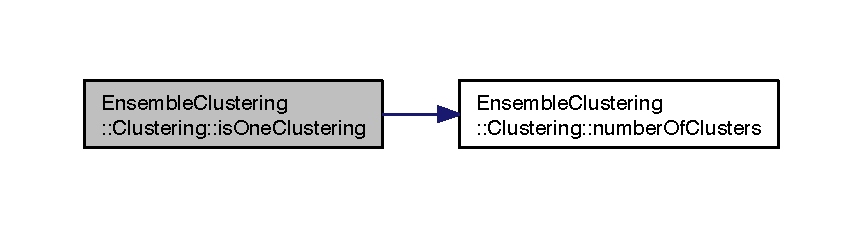
\includegraphics[width=350pt]{class_ensemble_clustering_1_1_clustering_ae00d7d11885b34c03969e213ec189a75_cgraph}
\end{center}
\end{figure}


\hypertarget{class_ensemble_clustering_1_1_clustering_a6ef2d3f0c4a53532067a140caa531449}{\index{Ensemble\-Clustering\-::\-Clustering@{Ensemble\-Clustering\-::\-Clustering}!is\-Proper@{is\-Proper}}
\index{is\-Proper@{is\-Proper}!EnsembleClustering::Clustering@{Ensemble\-Clustering\-::\-Clustering}}
\subsubsection[{is\-Proper}]{\setlength{\rightskip}{0pt plus 5cm}bool Ensemble\-Clustering\-::\-Clustering\-::is\-Proper (
\begin{DoxyParamCaption}
\item[{{\bf Graph} \&}]{G}
\end{DoxyParamCaption}
)}}\label{class_ensemble_clustering_1_1_clustering_a6ef2d3f0c4a53532067a140caa531449}


Check whether this clustering is a proper clustering of the graph, i.\-e. 

a disjoint partition of the whole node set. 

Definition at line 47 of file Clustering.\-cpp.



Here is the call graph for this function\-:
\nopagebreak
\begin{figure}[H]
\begin{center}
\leavevmode
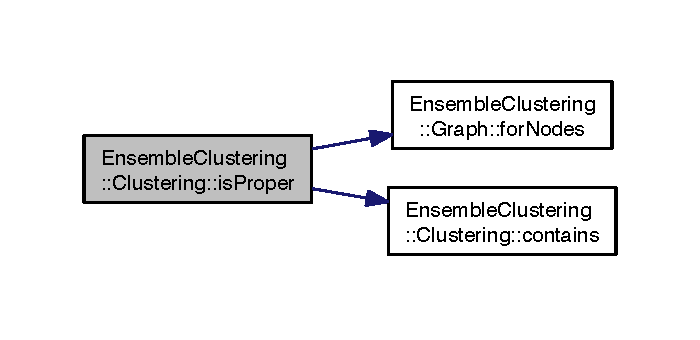
\includegraphics[width=336pt]{class_ensemble_clustering_1_1_clustering_a6ef2d3f0c4a53532067a140caa531449_cgraph}
\end{center}
\end{figure}


\hypertarget{class_ensemble_clustering_1_1_clustering_a49da98ece8e5e62638009ddf2cfa3929}{\index{Ensemble\-Clustering\-::\-Clustering@{Ensemble\-Clustering\-::\-Clustering}!is\-Singleton\-Clustering@{is\-Singleton\-Clustering}}
\index{is\-Singleton\-Clustering@{is\-Singleton\-Clustering}!EnsembleClustering::Clustering@{Ensemble\-Clustering\-::\-Clustering}}
\subsubsection[{is\-Singleton\-Clustering}]{\setlength{\rightskip}{0pt plus 5cm}bool Ensemble\-Clustering\-::\-Clustering\-::is\-Singleton\-Clustering (
\begin{DoxyParamCaption}
\item[{{\bf Graph} \&}]{G}
\end{DoxyParamCaption}
)}}\label{class_ensemble_clustering_1_1_clustering_a49da98ece8e5e62638009ddf2cfa3929}


Check if clustering is a singleton clustering, i.\-e. 

every node is assigned to a different cluster. 

Definition at line 114 of file Clustering.\-cpp.



Here is the call graph for this function\-:
\nopagebreak
\begin{figure}[H]
\begin{center}
\leavevmode
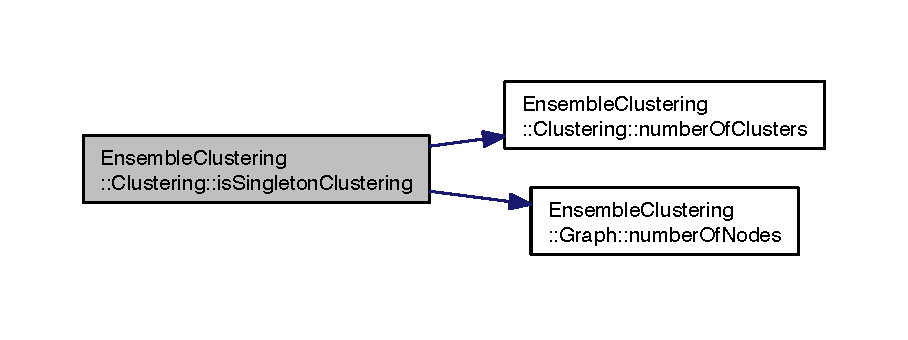
\includegraphics[width=350pt]{class_ensemble_clustering_1_1_clustering_a49da98ece8e5e62638009ddf2cfa3929_cgraph}
\end{center}
\end{figure}


\hypertarget{class_ensemble_clustering_1_1_clustering_ab64cf7248533ea358d7621ca8296b085}{\index{Ensemble\-Clustering\-::\-Clustering@{Ensemble\-Clustering\-::\-Clustering}!lower\-Bound@{lower\-Bound}}
\index{lower\-Bound@{lower\-Bound}!EnsembleClustering::Clustering@{Ensemble\-Clustering\-::\-Clustering}}
\subsubsection[{lower\-Bound}]{\setlength{\rightskip}{0pt plus 5cm}{\bf cluster} Ensemble\-Clustering\-::\-Clustering\-::lower\-Bound (
\begin{DoxyParamCaption}
{}
\end{DoxyParamCaption}
) const}}\label{class_ensemble_clustering_1_1_clustering_ab64cf7248533ea358d7621ca8296b085}


Return a lower bound for the cluster ids that have been assigned. 



Definition at line 76 of file Clustering.\-cpp.

\hypertarget{class_ensemble_clustering_1_1_clustering_a1cfe6fb096bef4aeb7814877847e2df9}{\index{Ensemble\-Clustering\-::\-Clustering@{Ensemble\-Clustering\-::\-Clustering}!merge\-Clusters@{merge\-Clusters}}
\index{merge\-Clusters@{merge\-Clusters}!EnsembleClustering::Clustering@{Ensemble\-Clustering\-::\-Clustering}}
\subsubsection[{merge\-Clusters}]{\setlength{\rightskip}{0pt plus 5cm}void Ensemble\-Clustering\-::\-Clustering\-::merge\-Clusters (
\begin{DoxyParamCaption}
\item[{{\bf cluster}}]{c, }
\item[{{\bf cluster}}]{d}
\end{DoxyParamCaption}
)}}\label{class_ensemble_clustering_1_1_clustering_a1cfe6fb096bef4aeb7814877847e2df9}


Assigns the nodes from both clusters to a new cluster. 



Definition at line 38 of file Clustering.\-cpp.



Here is the call graph for this function\-:
\nopagebreak
\begin{figure}[H]
\begin{center}
\leavevmode
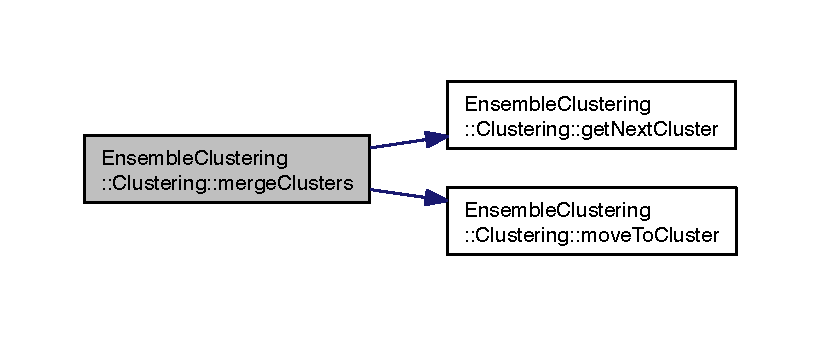
\includegraphics[width=350pt]{class_ensemble_clustering_1_1_clustering_a1cfe6fb096bef4aeb7814877847e2df9_cgraph}
\end{center}
\end{figure}


\hypertarget{class_ensemble_clustering_1_1_clustering_a7e3a719ed9904897617a3152bf80a634}{\index{Ensemble\-Clustering\-::\-Clustering@{Ensemble\-Clustering\-::\-Clustering}!move\-To\-Cluster@{move\-To\-Cluster}}
\index{move\-To\-Cluster@{move\-To\-Cluster}!EnsembleClustering::Clustering@{Ensemble\-Clustering\-::\-Clustering}}
\subsubsection[{move\-To\-Cluster}]{\setlength{\rightskip}{0pt plus 5cm}void Ensemble\-Clustering\-::\-Clustering\-::move\-To\-Cluster (
\begin{DoxyParamCaption}
\item[{{\bf cluster}}]{c, }
\item[{{\bf node}}]{u}
\end{DoxyParamCaption}
)}}\label{class_ensemble_clustering_1_1_clustering_a7e3a719ed9904897617a3152bf80a634}


Move a (previously assigned) node to a cluster. 



Definition at line 33 of file Clustering.\-cpp.

\hypertarget{class_ensemble_clustering_1_1_clustering_a7eb03661a933eff8176af0e073da2ef4}{\index{Ensemble\-Clustering\-::\-Clustering@{Ensemble\-Clustering\-::\-Clustering}!number\-Of\-Clusters@{number\-Of\-Clusters}}
\index{number\-Of\-Clusters@{number\-Of\-Clusters}!EnsembleClustering::Clustering@{Ensemble\-Clustering\-::\-Clustering}}
\subsubsection[{number\-Of\-Clusters}]{\setlength{\rightskip}{0pt plus 5cm}{\bf count} Ensemble\-Clustering\-::\-Clustering\-::number\-Of\-Clusters (
\begin{DoxyParamCaption}
{}
\end{DoxyParamCaption}
) const}}\label{class_ensemble_clustering_1_1_clustering_a7eb03661a933eff8176af0e073da2ef4}


Get the current number of clusters in this clustering. 



Definition at line 59 of file Clustering.\-cpp.

\hypertarget{class_ensemble_clustering_1_1_clustering_aaa9d16c93e56a4ea1c6bcf7eb302610a}{\index{Ensemble\-Clustering\-::\-Clustering@{Ensemble\-Clustering\-::\-Clustering}!operator\mbox{[}$\,$\mbox{]}@{operator[]}}
\index{operator\mbox{[}$\,$\mbox{]}@{operator[]}!EnsembleClustering::Clustering@{Ensemble\-Clustering\-::\-Clustering}}
\subsubsection[{operator[]}]{\setlength{\rightskip}{0pt plus 5cm}{\bf cluster}\& Ensemble\-Clustering\-::\-Clustering\-::operator\mbox{[}$\,$\mbox{]} (
\begin{DoxyParamCaption}
\item[{const {\bf node} \&}]{u}
\end{DoxyParamCaption}
)\hspace{0.3cm}{\ttfamily [inline]}}}\label{class_ensemble_clustering_1_1_clustering_aaa9d16c93e56a4ea1c6bcf7eb302610a}


Index operator. 


\begin{DoxyParams}[1]{Parameters}
\mbox{\tt in}  & {\em u} & a node \\
\hline
\end{DoxyParams}


Definition at line 71 of file Clustering.\-h.

\hypertarget{class_ensemble_clustering_1_1_clustering_aa277d9365e79e8b2f067e8630a29b031}{\index{Ensemble\-Clustering\-::\-Clustering@{Ensemble\-Clustering\-::\-Clustering}!operator\mbox{[}$\,$\mbox{]}@{operator[]}}
\index{operator\mbox{[}$\,$\mbox{]}@{operator[]}!EnsembleClustering::Clustering@{Ensemble\-Clustering\-::\-Clustering}}
\subsubsection[{operator[]}]{\setlength{\rightskip}{0pt plus 5cm}const {\bf cluster}\& Ensemble\-Clustering\-::\-Clustering\-::operator\mbox{[}$\,$\mbox{]} (
\begin{DoxyParamCaption}
\item[{const {\bf node} \&}]{u}
\end{DoxyParamCaption}
) const\hspace{0.3cm}{\ttfamily [inline]}}}\label{class_ensemble_clustering_1_1_clustering_aa277d9365e79e8b2f067e8630a29b031}


Index operator for const instances of this class. 


\begin{DoxyParams}[1]{Parameters}
\mbox{\tt in}  & {\em u} & a node \\
\hline
\end{DoxyParams}


Definition at line 79 of file Clustering.\-h.

\hypertarget{class_ensemble_clustering_1_1_clustering_ace9debc0ddc3de9f505ab33f9490c7c6}{\index{Ensemble\-Clustering\-::\-Clustering@{Ensemble\-Clustering\-::\-Clustering}!parallel\-For\-Entries@{parallel\-For\-Entries}}
\index{parallel\-For\-Entries@{parallel\-For\-Entries}!EnsembleClustering::Clustering@{Ensemble\-Clustering\-::\-Clustering}}
\subsubsection[{parallel\-For\-Entries}]{\setlength{\rightskip}{0pt plus 5cm}template$<$typename Callback $>$ void Ensemble\-Clustering\-::\-Clustering\-::parallel\-For\-Entries (
\begin{DoxyParamCaption}
\item[{Callback}]{handle}
\end{DoxyParamCaption}
)\hspace{0.3cm}{\ttfamily [inline]}}}\label{class_ensemble_clustering_1_1_clustering_ace9debc0ddc3de9f505ab33f9490c7c6}


Iterate over all entries (node, cluster) in parallel and execute callback function (lambda closure). 



Definition at line 234 of file Clustering.\-h.

\hypertarget{class_ensemble_clustering_1_1_clustering_a983184e9efa473931ae7dfc9c566e666}{\index{Ensemble\-Clustering\-::\-Clustering@{Ensemble\-Clustering\-::\-Clustering}!set\-Name@{set\-Name}}
\index{set\-Name@{set\-Name}!EnsembleClustering::Clustering@{Ensemble\-Clustering\-::\-Clustering}}
\subsubsection[{set\-Name}]{\setlength{\rightskip}{0pt plus 5cm}void Ensemble\-Clustering\-::\-Clustering\-::set\-Name (
\begin{DoxyParamCaption}
\item[{std\-::string}]{name}
\end{DoxyParamCaption}
)}}\label{class_ensemble_clustering_1_1_clustering_a983184e9efa473931ae7dfc9c566e666}


Set a human-\/readable identifier (vulg. 

a \char`\"{}name\char`\"{}) for the graph instance. 

Definition at line 102 of file Clustering.\-cpp.

\hypertarget{class_ensemble_clustering_1_1_clustering_adb704c4cbb2205b7858ac2d7f0f5014f}{\index{Ensemble\-Clustering\-::\-Clustering@{Ensemble\-Clustering\-::\-Clustering}!set\-Upper\-Bound@{set\-Upper\-Bound}}
\index{set\-Upper\-Bound@{set\-Upper\-Bound}!EnsembleClustering::Clustering@{Ensemble\-Clustering\-::\-Clustering}}
\subsubsection[{set\-Upper\-Bound}]{\setlength{\rightskip}{0pt plus 5cm}void Ensemble\-Clustering\-::\-Clustering\-::set\-Upper\-Bound (
\begin{DoxyParamCaption}
\item[{{\bf cluster}}]{id}
\end{DoxyParamCaption}
)}}\label{class_ensemble_clustering_1_1_clustering_adb704c4cbb2205b7858ac2d7f0f5014f}


Set an upper bound for the cluster ids. 



Definition at line 142 of file Clustering.\-cpp.

\hypertarget{class_ensemble_clustering_1_1_clustering_a461a251d674b64cf29e97408c343253a}{\index{Ensemble\-Clustering\-::\-Clustering@{Ensemble\-Clustering\-::\-Clustering}!to\-Singleton@{to\-Singleton}}
\index{to\-Singleton@{to\-Singleton}!EnsembleClustering::Clustering@{Ensemble\-Clustering\-::\-Clustering}}
\subsubsection[{to\-Singleton}]{\setlength{\rightskip}{0pt plus 5cm}void Ensemble\-Clustering\-::\-Clustering\-::to\-Singleton (
\begin{DoxyParamCaption}
\item[{{\bf node}}]{u}
\end{DoxyParamCaption}
)}}\label{class_ensemble_clustering_1_1_clustering_a461a251d674b64cf29e97408c343253a}


Creates a singleton cluster containing the node. 



Definition at line 29 of file Clustering.\-cpp.



Here is the call graph for this function\-:
\nopagebreak
\begin{figure}[H]
\begin{center}
\leavevmode
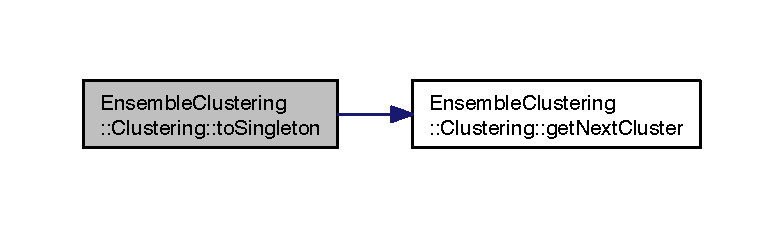
\includegraphics[width=350pt]{class_ensemble_clustering_1_1_clustering_a461a251d674b64cf29e97408c343253a_cgraph}
\end{center}
\end{figure}


\hypertarget{class_ensemble_clustering_1_1_clustering_ae0b22bda843f96f9428d05aa582cfe4b}{\index{Ensemble\-Clustering\-::\-Clustering@{Ensemble\-Clustering\-::\-Clustering}!upper\-Bound@{upper\-Bound}}
\index{upper\-Bound@{upper\-Bound}!EnsembleClustering::Clustering@{Ensemble\-Clustering\-::\-Clustering}}
\subsubsection[{upper\-Bound}]{\setlength{\rightskip}{0pt plus 5cm}{\bf cluster} Ensemble\-Clustering\-::\-Clustering\-::upper\-Bound (
\begin{DoxyParamCaption}
{}
\end{DoxyParamCaption}
) const}}\label{class_ensemble_clustering_1_1_clustering_ae0b22bda843f96f9428d05aa582cfe4b}


Return an upper bound for the cluster ids that have been assigned. 

(This is the maximum id + 1.) 

Definition at line 72 of file Clustering.\-cpp.



\subsection{Member Data Documentation}
\hypertarget{class_ensemble_clustering_1_1_clustering_affe0177a3d80ddd03d475307a74b3a1c}{\index{Ensemble\-Clustering\-::\-Clustering@{Ensemble\-Clustering\-::\-Clustering}!name@{name}}
\index{name@{name}!EnsembleClustering::Clustering@{Ensemble\-Clustering\-::\-Clustering}}
\subsubsection[{name}]{\setlength{\rightskip}{0pt plus 5cm}std\-::string Ensemble\-Clustering\-::\-Clustering\-::name\hspace{0.3cm}{\ttfamily [protected]}}}\label{class_ensemble_clustering_1_1_clustering_affe0177a3d80ddd03d475307a74b3a1c}


Definition at line 27 of file Clustering.\-h.

\hypertarget{class_ensemble_clustering_1_1_clustering_a47de59cf22e93a801cac55eb001b6d3d}{\index{Ensemble\-Clustering\-::\-Clustering@{Ensemble\-Clustering\-::\-Clustering}!next\-Cluster@{next\-Cluster}}
\index{next\-Cluster@{next\-Cluster}!EnsembleClustering::Clustering@{Ensemble\-Clustering\-::\-Clustering}}
\subsubsection[{next\-Cluster}]{\setlength{\rightskip}{0pt plus 5cm}{\bf cluster} Ensemble\-Clustering\-::\-Clustering\-::next\-Cluster\hspace{0.3cm}{\ttfamily [protected]}}}\label{class_ensemble_clustering_1_1_clustering_a47de59cf22e93a801cac55eb001b6d3d}


next free cluster id for new cluster 



Definition at line 26 of file Clustering.\-h.

\hypertarget{class_ensemble_clustering_1_1_clustering_a59e76a2bdf80c98186938c46814b9e36}{\index{Ensemble\-Clustering\-::\-Clustering@{Ensemble\-Clustering\-::\-Clustering}!upper\-Id\-Bound@{upper\-Id\-Bound}}
\index{upper\-Id\-Bound@{upper\-Id\-Bound}!EnsembleClustering::Clustering@{Ensemble\-Clustering\-::\-Clustering}}
\subsubsection[{upper\-Id\-Bound}]{\setlength{\rightskip}{0pt plus 5cm}{\bf cluster} Ensemble\-Clustering\-::\-Clustering\-::upper\-Id\-Bound\hspace{0.3cm}{\ttfamily [protected]}}}\label{class_ensemble_clustering_1_1_clustering_a59e76a2bdf80c98186938c46814b9e36}


upper bound for cluster ids 



Definition at line 28 of file Clustering.\-h.



The documentation for this class was generated from the following files\-:\begin{DoxyCompactItemize}
\item 
src/clustering/\hyperlink{_clustering_8h}{Clustering.\-h}\item 
src/clustering/\hyperlink{_clustering_8cpp}{Clustering.\-cpp}\end{DoxyCompactItemize}

\hypertarget{class_ensemble_clustering_1_1_clustering_generator}{\section{Ensemble\-Clustering\-:\-:Clustering\-Generator Class Reference}
\label{class_ensemble_clustering_1_1_clustering_generator}\index{Ensemble\-Clustering\-::\-Clustering\-Generator@{Ensemble\-Clustering\-::\-Clustering\-Generator}}
}


{\ttfamily \#include $<$Clustering\-Generator.\-h$>$}

\subsection*{Public Member Functions}
\begin{DoxyCompactItemize}
\item 
\hyperlink{class_ensemble_clustering_1_1_clustering_generator_ab0903498f00fe5fcf2f60e7c51c500f4}{Clustering\-Generator} ()
\item 
virtual \hyperlink{class_ensemble_clustering_1_1_clustering_generator_afd7d065d414d8f51fe584df2bc79577c}{$\sim$\-Clustering\-Generator} ()
\item 
virtual \hyperlink{class_ensemble_clustering_1_1_clustering}{Clustering} \& \hyperlink{class_ensemble_clustering_1_1_clustering_generator_a389692d091d311420c6173d1ae527f56}{make\-Singleton\-Clustering} (const \hyperlink{class_ensemble_clustering_1_1_graph}{Graph} \&G)
\begin{DoxyCompactList}\small\item\em Make a singleton clustering of G, i.\-e. \end{DoxyCompactList}\item 
virtual \hyperlink{class_ensemble_clustering_1_1_clustering}{Clustering} \& \hyperlink{class_ensemble_clustering_1_1_clustering_generator_aceff2507723f4a978f7bf51f0c3577be}{make\-One\-Clustering} (const \hyperlink{class_ensemble_clustering_1_1_graph}{Graph} \&G)
\begin{DoxyCompactList}\small\item\em Make a 1-\/clustering of G, i.\-e. \end{DoxyCompactList}\end{DoxyCompactItemize}


\subsection{Detailed Description}


Definition at line 15 of file Clustering\-Generator.\-h.



\subsection{Constructor \& Destructor Documentation}
\hypertarget{class_ensemble_clustering_1_1_clustering_generator_ab0903498f00fe5fcf2f60e7c51c500f4}{\index{Ensemble\-Clustering\-::\-Clustering\-Generator@{Ensemble\-Clustering\-::\-Clustering\-Generator}!Clustering\-Generator@{Clustering\-Generator}}
\index{Clustering\-Generator@{Clustering\-Generator}!EnsembleClustering::ClusteringGenerator@{Ensemble\-Clustering\-::\-Clustering\-Generator}}
\subsubsection[{Clustering\-Generator}]{\setlength{\rightskip}{0pt plus 5cm}Ensemble\-Clustering\-::\-Clustering\-Generator\-::\-Clustering\-Generator (
\begin{DoxyParamCaption}
{}
\end{DoxyParamCaption}
)}}\label{class_ensemble_clustering_1_1_clustering_generator_ab0903498f00fe5fcf2f60e7c51c500f4}


Definition at line 12 of file Clustering\-Generator.\-cpp.

\hypertarget{class_ensemble_clustering_1_1_clustering_generator_afd7d065d414d8f51fe584df2bc79577c}{\index{Ensemble\-Clustering\-::\-Clustering\-Generator@{Ensemble\-Clustering\-::\-Clustering\-Generator}!$\sim$\-Clustering\-Generator@{$\sim$\-Clustering\-Generator}}
\index{$\sim$\-Clustering\-Generator@{$\sim$\-Clustering\-Generator}!EnsembleClustering::ClusteringGenerator@{Ensemble\-Clustering\-::\-Clustering\-Generator}}
\subsubsection[{$\sim$\-Clustering\-Generator}]{\setlength{\rightskip}{0pt plus 5cm}Ensemble\-Clustering\-::\-Clustering\-Generator\-::$\sim$\-Clustering\-Generator (
\begin{DoxyParamCaption}
{}
\end{DoxyParamCaption}
)\hspace{0.3cm}{\ttfamily [virtual]}}}\label{class_ensemble_clustering_1_1_clustering_generator_afd7d065d414d8f51fe584df2bc79577c}


Definition at line 17 of file Clustering\-Generator.\-cpp.



\subsection{Member Function Documentation}
\hypertarget{class_ensemble_clustering_1_1_clustering_generator_aceff2507723f4a978f7bf51f0c3577be}{\index{Ensemble\-Clustering\-::\-Clustering\-Generator@{Ensemble\-Clustering\-::\-Clustering\-Generator}!make\-One\-Clustering@{make\-One\-Clustering}}
\index{make\-One\-Clustering@{make\-One\-Clustering}!EnsembleClustering::ClusteringGenerator@{Ensemble\-Clustering\-::\-Clustering\-Generator}}
\subsubsection[{make\-One\-Clustering}]{\setlength{\rightskip}{0pt plus 5cm}{\bf Clustering} \& Ensemble\-Clustering\-::\-Clustering\-Generator\-::make\-One\-Clustering (
\begin{DoxyParamCaption}
\item[{const {\bf Graph} \&}]{G}
\end{DoxyParamCaption}
)\hspace{0.3cm}{\ttfamily [virtual]}}}\label{class_ensemble_clustering_1_1_clustering_generator_aceff2507723f4a978f7bf51f0c3577be}


Make a 1-\/clustering of G, i.\-e. 

a clustering in which all nodes belong to the same cluster. 

Definition at line 30 of file Clustering\-Generator.\-cpp.



Here is the call graph for this function\-:\nopagebreak
\begin{figure}[H]
\begin{center}
\leavevmode
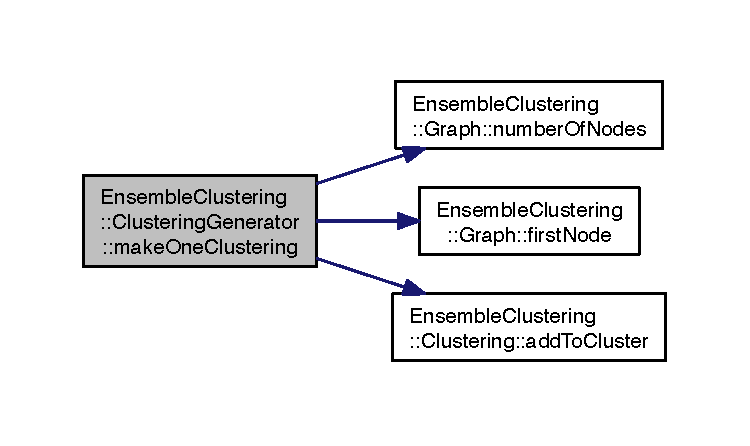
\includegraphics[width=350pt]{class_ensemble_clustering_1_1_clustering_generator_aceff2507723f4a978f7bf51f0c3577be_cgraph}
\end{center}
\end{figure}


\hypertarget{class_ensemble_clustering_1_1_clustering_generator_a389692d091d311420c6173d1ae527f56}{\index{Ensemble\-Clustering\-::\-Clustering\-Generator@{Ensemble\-Clustering\-::\-Clustering\-Generator}!make\-Singleton\-Clustering@{make\-Singleton\-Clustering}}
\index{make\-Singleton\-Clustering@{make\-Singleton\-Clustering}!EnsembleClustering::ClusteringGenerator@{Ensemble\-Clustering\-::\-Clustering\-Generator}}
\subsubsection[{make\-Singleton\-Clustering}]{\setlength{\rightskip}{0pt plus 5cm}{\bf Clustering} \& Ensemble\-Clustering\-::\-Clustering\-Generator\-::make\-Singleton\-Clustering (
\begin{DoxyParamCaption}
\item[{const {\bf Graph} \&}]{G}
\end{DoxyParamCaption}
)\hspace{0.3cm}{\ttfamily [virtual]}}}\label{class_ensemble_clustering_1_1_clustering_generator_a389692d091d311420c6173d1ae527f56}


Make a singleton clustering of G, i.\-e. 

a clustering in which every node belongs to its own cluster. 

Definition at line 21 of file Clustering\-Generator.\-cpp.



Here is the call graph for this function\-:\nopagebreak
\begin{figure}[H]
\begin{center}
\leavevmode
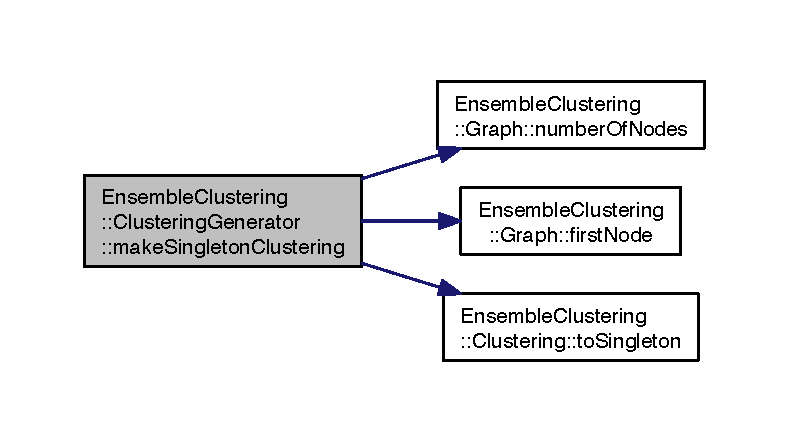
\includegraphics[width=350pt]{class_ensemble_clustering_1_1_clustering_generator_a389692d091d311420c6173d1ae527f56_cgraph}
\end{center}
\end{figure}




The documentation for this class was generated from the following files\-:\begin{DoxyCompactItemize}
\item 
src/clustering/\hyperlink{_clustering_generator_8h}{Clustering\-Generator.\-h}\item 
src/clustering/\hyperlink{_clustering_generator_8cpp}{Clustering\-Generator.\-cpp}\end{DoxyCompactItemize}

\hypertarget{class_ensemble_clustering_1_1_clustering_test}{\section{Ensemble\-Clustering\-:\-:Clustering\-Test Class Reference}
\label{class_ensemble_clustering_1_1_clustering_test}\index{Ensemble\-Clustering\-::\-Clustering\-Test@{Ensemble\-Clustering\-::\-Clustering\-Test}}
}


{\ttfamily \#include $<$Clustering\-Test.\-h$>$}



Inheritance diagram for Ensemble\-Clustering\-:\-:Clustering\-Test\-:\nopagebreak
\begin{figure}[H]
\begin{center}
\leavevmode
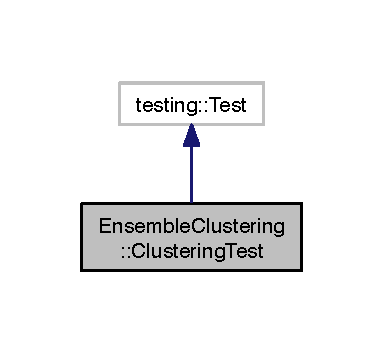
\includegraphics[width=184pt]{class_ensemble_clustering_1_1_clustering_test__inherit__graph}
\end{center}
\end{figure}


Collaboration diagram for Ensemble\-Clustering\-:\-:Clustering\-Test\-:\nopagebreak
\begin{figure}[H]
\begin{center}
\leavevmode
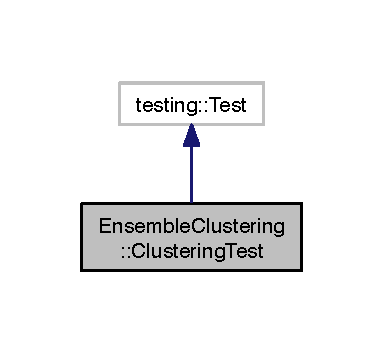
\includegraphics[width=184pt]{class_ensemble_clustering_1_1_clustering_test__coll__graph}
\end{center}
\end{figure}


\subsection{Detailed Description}


Definition at line 22 of file Clustering\-Test.\-h.



The documentation for this class was generated from the following file\-:\begin{DoxyCompactItemize}
\item 
src/clustering/test/\hyperlink{_clustering_test_8h}{Clustering\-Test.\-h}\end{DoxyCompactItemize}

\hypertarget{class_ensemble_clustering_1_1_contracter}{\section{Ensemble\-Clustering\-:\-:Contracter Class Reference}
\label{class_ensemble_clustering_1_1_contracter}\index{Ensemble\-Clustering\-::\-Contracter@{Ensemble\-Clustering\-::\-Contracter}}
}


{\ttfamily \#include $<$Contracter.\-h$>$}



Inheritance diagram for Ensemble\-Clustering\-:\-:Contracter\-:\nopagebreak
\begin{figure}[H]
\begin{center}
\leavevmode
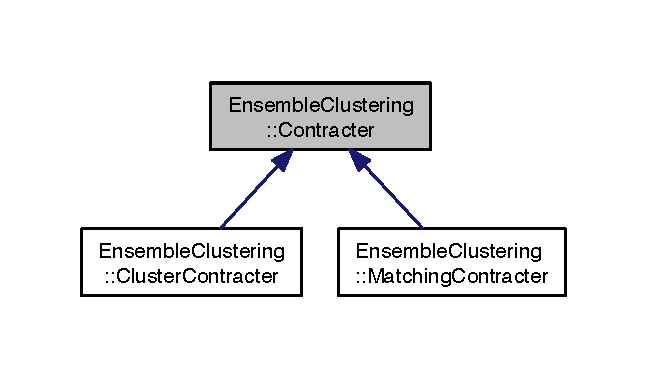
\includegraphics[width=184pt]{class_ensemble_clustering_1_1_contracter__inherit__graph}
\end{center}
\end{figure}
\subsection*{Public Member Functions}
\begin{DoxyCompactItemize}
\item 
\hyperlink{class_ensemble_clustering_1_1_contracter_a191a4d23919919852f13b6ea391bde1c}{Contracter} ()
\item 
virtual \hyperlink{class_ensemble_clustering_1_1_contracter_ad147c8a5d4e76dea9ab43a06b4ac4429}{$\sim$\-Contracter} ()
\item 
virtual \hyperlink{namespace_ensemble_clustering_ae829290aeccd1a420b17a37fd901f114}{node} \hyperlink{class_ensemble_clustering_1_1_contracter_a1f14b1abca4f219cfdf105cd4e032760}{contract} (\hyperlink{namespace_ensemble_clustering_ae829290aeccd1a420b17a37fd901f114}{node} u, \hyperlink{namespace_ensemble_clustering_ae829290aeccd1a420b17a37fd901f114}{node} v)
\end{DoxyCompactItemize}


\subsection{Detailed Description}


Definition at line 17 of file Contracter.\-h.



\subsection{Constructor \& Destructor Documentation}
\hypertarget{class_ensemble_clustering_1_1_contracter_a191a4d23919919852f13b6ea391bde1c}{\index{Ensemble\-Clustering\-::\-Contracter@{Ensemble\-Clustering\-::\-Contracter}!Contracter@{Contracter}}
\index{Contracter@{Contracter}!EnsembleClustering::Contracter@{Ensemble\-Clustering\-::\-Contracter}}
\subsubsection[{Contracter}]{\setlength{\rightskip}{0pt plus 5cm}Ensemble\-Clustering\-::\-Contracter\-::\-Contracter (
\begin{DoxyParamCaption}
{}
\end{DoxyParamCaption}
)}}\label{class_ensemble_clustering_1_1_contracter_a191a4d23919919852f13b6ea391bde1c}


Definition at line 12 of file Contracter.\-cpp.

\hypertarget{class_ensemble_clustering_1_1_contracter_ad147c8a5d4e76dea9ab43a06b4ac4429}{\index{Ensemble\-Clustering\-::\-Contracter@{Ensemble\-Clustering\-::\-Contracter}!$\sim$\-Contracter@{$\sim$\-Contracter}}
\index{$\sim$\-Contracter@{$\sim$\-Contracter}!EnsembleClustering::Contracter@{Ensemble\-Clustering\-::\-Contracter}}
\subsubsection[{$\sim$\-Contracter}]{\setlength{\rightskip}{0pt plus 5cm}Ensemble\-Clustering\-::\-Contracter\-::$\sim$\-Contracter (
\begin{DoxyParamCaption}
{}
\end{DoxyParamCaption}
)\hspace{0.3cm}{\ttfamily [virtual]}}}\label{class_ensemble_clustering_1_1_contracter_ad147c8a5d4e76dea9ab43a06b4ac4429}


Definition at line 17 of file Contracter.\-cpp.



\subsection{Member Function Documentation}
\hypertarget{class_ensemble_clustering_1_1_contracter_a1f14b1abca4f219cfdf105cd4e032760}{\index{Ensemble\-Clustering\-::\-Contracter@{Ensemble\-Clustering\-::\-Contracter}!contract@{contract}}
\index{contract@{contract}!EnsembleClustering::Contracter@{Ensemble\-Clustering\-::\-Contracter}}
\subsubsection[{contract}]{\setlength{\rightskip}{0pt plus 5cm}{\bf node} Ensemble\-Clustering\-::\-Contracter\-::contract (
\begin{DoxyParamCaption}
\item[{{\bf node}}]{u, }
\item[{{\bf node}}]{v}
\end{DoxyParamCaption}
)\hspace{0.3cm}{\ttfamily [virtual]}}}\label{class_ensemble_clustering_1_1_contracter_a1f14b1abca4f219cfdf105cd4e032760}


Definition at line 21 of file Contracter.\-cpp.



The documentation for this class was generated from the following files\-:\begin{DoxyCompactItemize}
\item 
src/coarsening/\hyperlink{_contracter_8h}{Contracter.\-h}\item 
src/coarsening/\hyperlink{_contracter_8cpp}{Contracter.\-cpp}\end{DoxyCompactItemize}

\hypertarget{class_ensemble_clustering_1_1_edge_scoring}{\section{Ensemble\-Clustering\-:\-:Edge\-Scoring Class Reference}
\label{class_ensemble_clustering_1_1_edge_scoring}\index{Ensemble\-Clustering\-::\-Edge\-Scoring@{Ensemble\-Clustering\-::\-Edge\-Scoring}}
}


{\ttfamily \#include $<$Edge\-Scoring.\-h$>$}



Inheritance diagram for Ensemble\-Clustering\-:\-:Edge\-Scoring\-:\nopagebreak
\begin{figure}[H]
\begin{center}
\leavevmode
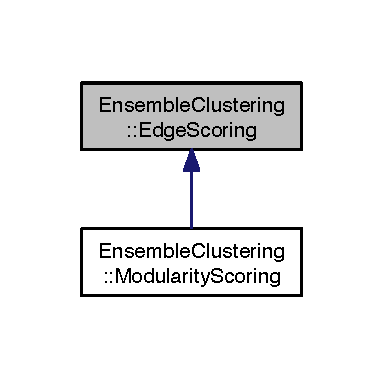
\includegraphics[width=184pt]{class_ensemble_clustering_1_1_edge_scoring__inherit__graph}
\end{center}
\end{figure}
\subsection*{Public Member Functions}
\begin{DoxyCompactItemize}
\item 
\hyperlink{class_ensemble_clustering_1_1_edge_scoring_a83339193ebf55255b09a34a2e1112eea}{Edge\-Scoring} ()
\item 
virtual \hyperlink{class_ensemble_clustering_1_1_edge_scoring_a1bb790ce6fd801ea40e0603785c73727}{$\sim$\-Edge\-Scoring} ()
\item 
virtual double \hyperlink{class_ensemble_clustering_1_1_edge_scoring_ae0b8ed83c76ea8f71f8246949d3106f4}{score\-Edge} (\hyperlink{namespace_ensemble_clustering_a136bcdc52fb2f62a89bc8bf8c1a7cb8f}{Node} u, \hyperlink{namespace_ensemble_clustering_a136bcdc52fb2f62a89bc8bf8c1a7cb8f}{Node} v)=0
\end{DoxyCompactItemize}


\subsection{Detailed Description}


Definition at line 16 of file Edge\-Scoring.\-h.



\subsection{Constructor \& Destructor Documentation}
\hypertarget{class_ensemble_clustering_1_1_edge_scoring_a83339193ebf55255b09a34a2e1112eea}{\index{Ensemble\-Clustering\-::\-Edge\-Scoring@{Ensemble\-Clustering\-::\-Edge\-Scoring}!Edge\-Scoring@{Edge\-Scoring}}
\index{Edge\-Scoring@{Edge\-Scoring}!EnsembleClustering::EdgeScoring@{Ensemble\-Clustering\-::\-Edge\-Scoring}}
\subsubsection[{Edge\-Scoring}]{\setlength{\rightskip}{0pt plus 5cm}Ensemble\-Clustering\-::\-Edge\-Scoring\-::\-Edge\-Scoring (
\begin{DoxyParamCaption}
{}
\end{DoxyParamCaption}
)}}\label{class_ensemble_clustering_1_1_edge_scoring_a83339193ebf55255b09a34a2e1112eea}


Definition at line 12 of file Edge\-Scoring.\-cpp.

\hypertarget{class_ensemble_clustering_1_1_edge_scoring_a1bb790ce6fd801ea40e0603785c73727}{\index{Ensemble\-Clustering\-::\-Edge\-Scoring@{Ensemble\-Clustering\-::\-Edge\-Scoring}!$\sim$\-Edge\-Scoring@{$\sim$\-Edge\-Scoring}}
\index{$\sim$\-Edge\-Scoring@{$\sim$\-Edge\-Scoring}!EnsembleClustering::EdgeScoring@{Ensemble\-Clustering\-::\-Edge\-Scoring}}
\subsubsection[{$\sim$\-Edge\-Scoring}]{\setlength{\rightskip}{0pt plus 5cm}Ensemble\-Clustering\-::\-Edge\-Scoring\-::$\sim$\-Edge\-Scoring (
\begin{DoxyParamCaption}
{}
\end{DoxyParamCaption}
)\hspace{0.3cm}{\ttfamily [virtual]}}}\label{class_ensemble_clustering_1_1_edge_scoring_a1bb790ce6fd801ea40e0603785c73727}


Definition at line 17 of file Edge\-Scoring.\-cpp.



\subsection{Member Function Documentation}
\hypertarget{class_ensemble_clustering_1_1_edge_scoring_ae0b8ed83c76ea8f71f8246949d3106f4}{\index{Ensemble\-Clustering\-::\-Edge\-Scoring@{Ensemble\-Clustering\-::\-Edge\-Scoring}!score\-Edge@{score\-Edge}}
\index{score\-Edge@{score\-Edge}!EnsembleClustering::EdgeScoring@{Ensemble\-Clustering\-::\-Edge\-Scoring}}
\subsubsection[{score\-Edge}]{\setlength{\rightskip}{0pt plus 5cm}virtual double Ensemble\-Clustering\-::\-Edge\-Scoring\-::score\-Edge (
\begin{DoxyParamCaption}
\item[{{\bf Node}}]{u, }
\item[{{\bf Node}}]{v}
\end{DoxyParamCaption}
)\hspace{0.3cm}{\ttfamily [pure virtual]}}}\label{class_ensemble_clustering_1_1_edge_scoring_ae0b8ed83c76ea8f71f8246949d3106f4}


The documentation for this class was generated from the following files\-:\begin{DoxyCompactItemize}
\item 
src/scoring/\hyperlink{_edge_scoring_8h}{Edge\-Scoring.\-h}\item 
src/scoring/\hyperlink{_edge_scoring_8cpp}{Edge\-Scoring.\-cpp}\end{DoxyCompactItemize}

\hypertarget{class_ensemble_clustering_1_1_ensemble_clusterer}{\section{Ensemble\-Clustering\-:\-:Ensemble\-Clusterer Class Reference}
\label{class_ensemble_clustering_1_1_ensemble_clusterer}\index{Ensemble\-Clustering\-::\-Ensemble\-Clusterer@{Ensemble\-Clustering\-::\-Ensemble\-Clusterer}}
}


{\ttfamily \#include $<$Ensemble\-Clusterer.\-h$>$}

\subsection*{Public Member Functions}
\begin{DoxyCompactItemize}
\item 
\hyperlink{class_ensemble_clustering_1_1_ensemble_clusterer_a09ad2e9d9f814df8905199f445b36448}{Ensemble\-Clusterer} ()
\item 
virtual \hyperlink{class_ensemble_clustering_1_1_ensemble_clusterer_ace47f754325f57fadd927c4f8379f51d}{$\sim$\-Ensemble\-Clusterer} ()
\end{DoxyCompactItemize}


\subsection{Detailed Description}


Definition at line 13 of file Ensemble\-Clusterer.\-h.



\subsection{Constructor \& Destructor Documentation}
\hypertarget{class_ensemble_clustering_1_1_ensemble_clusterer_a09ad2e9d9f814df8905199f445b36448}{\index{Ensemble\-Clustering\-::\-Ensemble\-Clusterer@{Ensemble\-Clustering\-::\-Ensemble\-Clusterer}!Ensemble\-Clusterer@{Ensemble\-Clusterer}}
\index{Ensemble\-Clusterer@{Ensemble\-Clusterer}!EnsembleClustering::EnsembleClusterer@{Ensemble\-Clustering\-::\-Ensemble\-Clusterer}}
\subsubsection[{Ensemble\-Clusterer}]{\setlength{\rightskip}{0pt plus 5cm}Ensemble\-Clustering\-::\-Ensemble\-Clusterer\-::\-Ensemble\-Clusterer (
\begin{DoxyParamCaption}
{}
\end{DoxyParamCaption}
)}}\label{class_ensemble_clustering_1_1_ensemble_clusterer_a09ad2e9d9f814df8905199f445b36448}


Definition at line 12 of file Ensemble\-Clusterer.\-cpp.

\hypertarget{class_ensemble_clustering_1_1_ensemble_clusterer_ace47f754325f57fadd927c4f8379f51d}{\index{Ensemble\-Clustering\-::\-Ensemble\-Clusterer@{Ensemble\-Clustering\-::\-Ensemble\-Clusterer}!$\sim$\-Ensemble\-Clusterer@{$\sim$\-Ensemble\-Clusterer}}
\index{$\sim$\-Ensemble\-Clusterer@{$\sim$\-Ensemble\-Clusterer}!EnsembleClustering::EnsembleClusterer@{Ensemble\-Clustering\-::\-Ensemble\-Clusterer}}
\subsubsection[{$\sim$\-Ensemble\-Clusterer}]{\setlength{\rightskip}{0pt plus 5cm}Ensemble\-Clustering\-::\-Ensemble\-Clusterer\-::$\sim$\-Ensemble\-Clusterer (
\begin{DoxyParamCaption}
{}
\end{DoxyParamCaption}
)\hspace{0.3cm}{\ttfamily [virtual]}}}\label{class_ensemble_clustering_1_1_ensemble_clusterer_ace47f754325f57fadd927c4f8379f51d}


Definition at line 17 of file Ensemble\-Clusterer.\-cpp.



The documentation for this class was generated from the following files\-:\begin{DoxyCompactItemize}
\item 
src/ensemble/\hyperlink{_ensemble_clusterer_8h}{Ensemble\-Clusterer.\-h}\item 
src/ensemble/\hyperlink{_ensemble_clusterer_8cpp}{Ensemble\-Clusterer.\-cpp}\end{DoxyCompactItemize}

\hypertarget{class_ensemble_clustering_1_1_graph}{\section{Ensemble\-Clustering\-:\-:Graph Class Reference}
\label{class_ensemble_clustering_1_1_graph}\index{Ensemble\-Clustering\-::\-Graph@{Ensemble\-Clustering\-::\-Graph}}
}


\hyperlink{class_ensemble_clustering_1_1_graph}{Graph} interface.  




{\ttfamily \#include $<$Graph.\-h$>$}

\subsection*{Public Member Functions}
\begin{DoxyCompactItemize}
\item 
\hyperlink{class_ensemble_clustering_1_1_graph_a65031e76ae95333341f795fb9a13647f}{Graph} ()
\begin{DoxyCompactList}\small\item\em methods \end{DoxyCompactList}\item 
\hyperlink{class_ensemble_clustering_1_1_graph_a0ffcdfea431e8c85de2058a226a4783a}{Graph} (stinger $\ast$\hyperlink{class_ensemble_clustering_1_1_graph_af83709e85afb91c70729405a725afb9a}{stinger\-G})
\begin{DoxyCompactList}\small\item\em Initialize with S\-T\-I\-N\-G\-E\-R graph. \end{DoxyCompactList}\item 
\hyperlink{class_ensemble_clustering_1_1_graph_ac8368ff972ce067d51e37c48124a0038}{$\sim$\-Graph} ()
\item 
stinger $\ast$ \hyperlink{class_ensemble_clustering_1_1_graph_ad7ad5a71649990fe2b823b8ed7a113b7}{as\-S\-T\-I\-N\-G\-E\-R} () const 
\begin{DoxyCompactList}\small\item\em Return the internal S\-T\-I\-N\-G\-E\-R data structure. \end{DoxyCompactList}\item 
void \hyperlink{class_ensemble_clustering_1_1_graph_a78d527f03a3a860ee173dadbaefe1d5c}{insert\-Edge} (\hyperlink{namespace_ensemble_clustering_ae829290aeccd1a420b17a37fd901f114}{node} u, \hyperlink{namespace_ensemble_clustering_ae829290aeccd1a420b17a37fd901f114}{node} v, double \hyperlink{class_ensemble_clustering_1_1_graph_a9bff231567f9ac604f1854d62f6682d1}{weight}=\hyperlink{class_ensemble_clustering_1_1_graph_a8186ee969064a4e12b779b1dc506ac60}{default\-Edge\-Weight}, int64\-\_\-t type=\hyperlink{class_ensemble_clustering_1_1_graph_a377621f37c1dc58f32ecec0fd229408e}{default\-Edge\-Type}, int64\-\_\-t timestamp=\hyperlink{class_ensemble_clustering_1_1_graph_a9a6623d55f673a3b30e0c23284dd6da1}{default\-Time\-Stamp})
\begin{DoxyCompactList}\small\item\em Insert a weighted, undirected edge. \end{DoxyCompactList}\item 
bool \hyperlink{class_ensemble_clustering_1_1_graph_a9be0c0a70204723e4b040b9cba51b15d}{has\-Edge} (\hyperlink{namespace_ensemble_clustering_ae829290aeccd1a420b17a37fd901f114}{node} u, \hyperlink{namespace_ensemble_clustering_ae829290aeccd1a420b17a37fd901f114}{node} v) const 
\begin{DoxyCompactList}\small\item\em Check if undirected edge \{u,v\} exists in G. \end{DoxyCompactList}\item 
double \hyperlink{class_ensemble_clustering_1_1_graph_a9bff231567f9ac604f1854d62f6682d1}{weight} (\hyperlink{namespace_ensemble_clustering_ae829290aeccd1a420b17a37fd901f114}{node} v) const 
\begin{DoxyCompactList}\small\item\em Return node weight. \end{DoxyCompactList}\item 
double \hyperlink{class_ensemble_clustering_1_1_graph_a656f5cb3119dd3f8f4182d38cce82fa0}{weight} (\hyperlink{namespace_ensemble_clustering_aff19dd5e3051ee3d4360fd3f29daf16b}{edge} uv) const 
\begin{DoxyCompactList}\small\item\em Return edge weight. \end{DoxyCompactList}\item 
double \hyperlink{class_ensemble_clustering_1_1_graph_a4699131f4d3602ecda00eaf70a86cbea}{weight} (\hyperlink{namespace_ensemble_clustering_ae829290aeccd1a420b17a37fd901f114}{node} u, \hyperlink{namespace_ensemble_clustering_ae829290aeccd1a420b17a37fd901f114}{node} v) const 
\begin{DoxyCompactList}\small\item\em Return edge weight. \end{DoxyCompactList}\item 
double \hyperlink{class_ensemble_clustering_1_1_graph_a7be7f13f5a31b0513293e7bbac26ca6c}{total\-Edge\-Weight} () const 
\begin{DoxyCompactList}\small\item\em Get the sum of the weight of all edges. \end{DoxyCompactList}\item 
int64\-\_\-t \hyperlink{class_ensemble_clustering_1_1_graph_a35f4b169cd0157117b468b1863a0d70a}{degree} (\hyperlink{namespace_ensemble_clustering_ae829290aeccd1a420b17a37fd901f114}{node} u) const 
\begin{DoxyCompactList}\small\item\em Return the degree (number of incident edges). \end{DoxyCompactList}\item 
int64\-\_\-t \hyperlink{class_ensemble_clustering_1_1_graph_ab019840b239c3247eaf00e5ffcc6bb03}{number\-Of\-Edges} () const 
\begin{DoxyCompactList}\small\item\em Return the number of edges in the graph. \end{DoxyCompactList}\item 
int64\-\_\-t \hyperlink{class_ensemble_clustering_1_1_graph_affe61a24e54266aba872272fb9501c61}{number\-Of\-Nodes} () const 
\begin{DoxyCompactList}\small\item\em Return the number of (non-\/isolated) nodes in the graph. \end{DoxyCompactList}\item 
\hyperlink{namespace_ensemble_clustering_ae829290aeccd1a420b17a37fd901f114}{node} \hyperlink{class_ensemble_clustering_1_1_graph_aaac8bcc5d64461cba54ad38ec929be3c}{first\-Node} () const 
\begin{DoxyCompactList}\small\item\em Get the first node index (for iteration over all nodes) \end{DoxyCompactList}\item 
\hyperlink{namespace_ensemble_clustering_ae829290aeccd1a420b17a37fd901f114}{node} \hyperlink{class_ensemble_clustering_1_1_graph_a3d6fe2d0c27605f4b55585198eb9b933}{last\-Node} () const 
\begin{DoxyCompactList}\small\item\em Get the last node index (for iteration over all nodes). \end{DoxyCompactList}\item 
{\footnotesize template$<$typename Callback $>$ }\\void \hyperlink{class_ensemble_clustering_1_1_graph_a7b599771f8dc476712ea7e6b52157a3f}{forall\-Edges} (bool parallel, Callback callback)
\end{DoxyCompactItemize}
\subsection*{Static Public Attributes}
\begin{DoxyCompactItemize}
\item 
static constexpr double \hyperlink{class_ensemble_clustering_1_1_graph_a8186ee969064a4e12b779b1dc506ac60}{default\-Edge\-Weight} = 1.\-0
\begin{DoxyCompactList}\small\item\em default parameters \end{DoxyCompactList}\item 
static const int64\-\_\-t \hyperlink{class_ensemble_clustering_1_1_graph_a377621f37c1dc58f32ecec0fd229408e}{default\-Edge\-Type} = 0
\item 
static const int64\-\_\-t \hyperlink{class_ensemble_clustering_1_1_graph_a9a6623d55f673a3b30e0c23284dd6da1}{default\-Time\-Stamp} = 0
\end{DoxyCompactItemize}
\subsection*{Protected Attributes}
\begin{DoxyCompactItemize}
\item 
stinger $\ast$ \hyperlink{class_ensemble_clustering_1_1_graph_af83709e85afb91c70729405a725afb9a}{stinger\-G}
\end{DoxyCompactItemize}


\subsection{Detailed Description}
\hyperlink{class_ensemble_clustering_1_1_graph}{Graph} interface. 

\hyperlink{class_ensemble_clustering_1_1_graph}{Graph} encapsulates a S\-T\-I\-N\-G\-E\-R graph object and provides a more concise interface to it.

The graph concept modelled is
\begin{DoxyItemize}
\item undirected
\item weighted
\item without self-\/loops (use node weights instead) 
\end{DoxyItemize}

Definition at line 77 of file Graph.\-h.



\subsection{Constructor \& Destructor Documentation}
\hypertarget{class_ensemble_clustering_1_1_graph_a65031e76ae95333341f795fb9a13647f}{\index{Ensemble\-Clustering\-::\-Graph@{Ensemble\-Clustering\-::\-Graph}!Graph@{Graph}}
\index{Graph@{Graph}!EnsembleClustering::Graph@{Ensemble\-Clustering\-::\-Graph}}
\subsubsection[{Graph}]{\setlength{\rightskip}{0pt plus 5cm}Ensemble\-Clustering\-::\-Graph\-::\-Graph (
\begin{DoxyParamCaption}
{}
\end{DoxyParamCaption}
)}}\label{class_ensemble_clustering_1_1_graph_a65031e76ae95333341f795fb9a13647f}


methods 

Construct \hyperlink{class_ensemble_clustering_1_1_graph}{Graph} object with new S\-T\-I\-N\-G\-E\-R graph inside. 

Definition at line 13 of file Graph.\-cpp.

\hypertarget{class_ensemble_clustering_1_1_graph_a0ffcdfea431e8c85de2058a226a4783a}{\index{Ensemble\-Clustering\-::\-Graph@{Ensemble\-Clustering\-::\-Graph}!Graph@{Graph}}
\index{Graph@{Graph}!EnsembleClustering::Graph@{Ensemble\-Clustering\-::\-Graph}}
\subsubsection[{Graph}]{\setlength{\rightskip}{0pt plus 5cm}Ensemble\-Clustering\-::\-Graph\-::\-Graph (
\begin{DoxyParamCaption}
\item[{stinger $\ast$}]{stinger\-G}
\end{DoxyParamCaption}
)}}\label{class_ensemble_clustering_1_1_graph_a0ffcdfea431e8c85de2058a226a4783a}


Initialize with S\-T\-I\-N\-G\-E\-R graph. 


\begin{DoxyParams}[1]{Parameters}
\mbox{\tt in}  & {\em stinger\-G} & a S\-T\-I\-N\-G\-E\-R graph struct \\
\hline
\end{DoxyParams}


Definition at line 20 of file Graph.\-cpp.

\hypertarget{class_ensemble_clustering_1_1_graph_ac8368ff972ce067d51e37c48124a0038}{\index{Ensemble\-Clustering\-::\-Graph@{Ensemble\-Clustering\-::\-Graph}!$\sim$\-Graph@{$\sim$\-Graph}}
\index{$\sim$\-Graph@{$\sim$\-Graph}!EnsembleClustering::Graph@{Ensemble\-Clustering\-::\-Graph}}
\subsubsection[{$\sim$\-Graph}]{\setlength{\rightskip}{0pt plus 5cm}Ensemble\-Clustering\-::\-Graph\-::$\sim$\-Graph (
\begin{DoxyParamCaption}
{}
\end{DoxyParamCaption}
)}}\label{class_ensemble_clustering_1_1_graph_ac8368ff972ce067d51e37c48124a0038}


Definition at line 17 of file Graph.\-cpp.



\subsection{Member Function Documentation}
\hypertarget{class_ensemble_clustering_1_1_graph_ad7ad5a71649990fe2b823b8ed7a113b7}{\index{Ensemble\-Clustering\-::\-Graph@{Ensemble\-Clustering\-::\-Graph}!as\-S\-T\-I\-N\-G\-E\-R@{as\-S\-T\-I\-N\-G\-E\-R}}
\index{as\-S\-T\-I\-N\-G\-E\-R@{as\-S\-T\-I\-N\-G\-E\-R}!EnsembleClustering::Graph@{Ensemble\-Clustering\-::\-Graph}}
\subsubsection[{as\-S\-T\-I\-N\-G\-E\-R}]{\setlength{\rightskip}{0pt plus 5cm}stinger $\ast$ Ensemble\-Clustering\-::\-Graph\-::as\-S\-T\-I\-N\-G\-E\-R (
\begin{DoxyParamCaption}
{}
\end{DoxyParamCaption}
) const}}\label{class_ensemble_clustering_1_1_graph_ad7ad5a71649990fe2b823b8ed7a113b7}


Return the internal S\-T\-I\-N\-G\-E\-R data structure. 



Definition at line 26 of file Graph.\-cpp.

\hypertarget{class_ensemble_clustering_1_1_graph_a35f4b169cd0157117b468b1863a0d70a}{\index{Ensemble\-Clustering\-::\-Graph@{Ensemble\-Clustering\-::\-Graph}!degree@{degree}}
\index{degree@{degree}!EnsembleClustering::Graph@{Ensemble\-Clustering\-::\-Graph}}
\subsubsection[{degree}]{\setlength{\rightskip}{0pt plus 5cm}int64\-\_\-t Ensemble\-Clustering\-::\-Graph\-::degree (
\begin{DoxyParamCaption}
\item[{{\bf node}}]{u}
\end{DoxyParamCaption}
) const}}\label{class_ensemble_clustering_1_1_graph_a35f4b169cd0157117b468b1863a0d70a}


Return the degree (number of incident edges). 



Definition at line 69 of file Graph.\-cpp.

\hypertarget{class_ensemble_clustering_1_1_graph_aaac8bcc5d64461cba54ad38ec929be3c}{\index{Ensemble\-Clustering\-::\-Graph@{Ensemble\-Clustering\-::\-Graph}!first\-Node@{first\-Node}}
\index{first\-Node@{first\-Node}!EnsembleClustering::Graph@{Ensemble\-Clustering\-::\-Graph}}
\subsubsection[{first\-Node}]{\setlength{\rightskip}{0pt plus 5cm}{\bf node} Ensemble\-Clustering\-::\-Graph\-::first\-Node (
\begin{DoxyParamCaption}
{}
\end{DoxyParamCaption}
) const}}\label{class_ensemble_clustering_1_1_graph_aaac8bcc5d64461cba54ad38ec929be3c}


Get the first node index (for iteration over all nodes) 



Definition at line 65 of file Graph.\-cpp.

\hypertarget{class_ensemble_clustering_1_1_graph_a7b599771f8dc476712ea7e6b52157a3f}{\index{Ensemble\-Clustering\-::\-Graph@{Ensemble\-Clustering\-::\-Graph}!forall\-Edges@{forall\-Edges}}
\index{forall\-Edges@{forall\-Edges}!EnsembleClustering::Graph@{Ensemble\-Clustering\-::\-Graph}}
\subsubsection[{forall\-Edges}]{\setlength{\rightskip}{0pt plus 5cm}template$<$typename Callback $>$ void Ensemble\-Clustering\-::\-Graph\-::forall\-Edges (
\begin{DoxyParamCaption}
\item[{bool}]{parallel, }
\item[{Callback}]{callback}
\end{DoxyParamCaption}
)\hspace{0.3cm}{\ttfamily [inline]}}}\label{class_ensemble_clustering_1_1_graph_a7b599771f8dc476712ea7e6b52157a3f}


Definition at line 195 of file Graph.\-h.

\hypertarget{class_ensemble_clustering_1_1_graph_a9be0c0a70204723e4b040b9cba51b15d}{\index{Ensemble\-Clustering\-::\-Graph@{Ensemble\-Clustering\-::\-Graph}!has\-Edge@{has\-Edge}}
\index{has\-Edge@{has\-Edge}!EnsembleClustering::Graph@{Ensemble\-Clustering\-::\-Graph}}
\subsubsection[{has\-Edge}]{\setlength{\rightskip}{0pt plus 5cm}bool Ensemble\-Clustering\-::\-Graph\-::has\-Edge (
\begin{DoxyParamCaption}
\item[{{\bf node}}]{u, }
\item[{{\bf node}}]{v}
\end{DoxyParamCaption}
) const}}\label{class_ensemble_clustering_1_1_graph_a9be0c0a70204723e4b040b9cba51b15d}


Check if undirected edge \{u,v\} exists in G. 



Definition at line 36 of file Graph.\-cpp.

\hypertarget{class_ensemble_clustering_1_1_graph_a78d527f03a3a860ee173dadbaefe1d5c}{\index{Ensemble\-Clustering\-::\-Graph@{Ensemble\-Clustering\-::\-Graph}!insert\-Edge@{insert\-Edge}}
\index{insert\-Edge@{insert\-Edge}!EnsembleClustering::Graph@{Ensemble\-Clustering\-::\-Graph}}
\subsubsection[{insert\-Edge}]{\setlength{\rightskip}{0pt plus 5cm}void Ensemble\-Clustering\-::\-Graph\-::insert\-Edge (
\begin{DoxyParamCaption}
\item[{{\bf node}}]{u, }
\item[{{\bf node}}]{v, }
\item[{double}]{weight = {\ttfamily {\bf default\-Edge\-Weight}}, }
\item[{int64\-\_\-t}]{type = {\ttfamily {\bf default\-Edge\-Type}}, }
\item[{int64\-\_\-t}]{timestamp = {\ttfamily {\bf default\-Time\-Stamp}}}
\end{DoxyParamCaption}
)}}\label{class_ensemble_clustering_1_1_graph_a78d527f03a3a860ee173dadbaefe1d5c}


Insert a weighted, undirected edge. 



Definition at line 30 of file Graph.\-cpp.

\hypertarget{class_ensemble_clustering_1_1_graph_a3d6fe2d0c27605f4b55585198eb9b933}{\index{Ensemble\-Clustering\-::\-Graph@{Ensemble\-Clustering\-::\-Graph}!last\-Node@{last\-Node}}
\index{last\-Node@{last\-Node}!EnsembleClustering::Graph@{Ensemble\-Clustering\-::\-Graph}}
\subsubsection[{last\-Node}]{\setlength{\rightskip}{0pt plus 5cm}{\bf node} Ensemble\-Clustering\-::\-Graph\-::last\-Node (
\begin{DoxyParamCaption}
{}
\end{DoxyParamCaption}
) const}}\label{class_ensemble_clustering_1_1_graph_a3d6fe2d0c27605f4b55585198eb9b933}


Get the last node index (for iteration over all nodes). 



Definition at line 85 of file Graph.\-cpp.



Here is the call graph for this function\-:\nopagebreak
\begin{figure}[H]
\begin{center}
\leavevmode
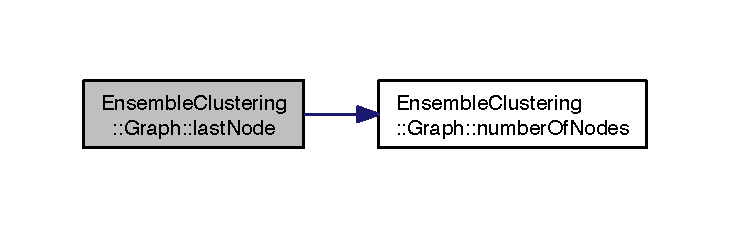
\includegraphics[width=350pt]{class_ensemble_clustering_1_1_graph_a3d6fe2d0c27605f4b55585198eb9b933_cgraph}
\end{center}
\end{figure}


\hypertarget{class_ensemble_clustering_1_1_graph_ab019840b239c3247eaf00e5ffcc6bb03}{\index{Ensemble\-Clustering\-::\-Graph@{Ensemble\-Clustering\-::\-Graph}!number\-Of\-Edges@{number\-Of\-Edges}}
\index{number\-Of\-Edges@{number\-Of\-Edges}!EnsembleClustering::Graph@{Ensemble\-Clustering\-::\-Graph}}
\subsubsection[{number\-Of\-Edges}]{\setlength{\rightskip}{0pt plus 5cm}int64\-\_\-t Ensemble\-Clustering\-::\-Graph\-::number\-Of\-Edges (
\begin{DoxyParamCaption}
{}
\end{DoxyParamCaption}
) const}}\label{class_ensemble_clustering_1_1_graph_ab019840b239c3247eaf00e5ffcc6bb03}


Return the number of edges in the graph. 



Definition at line 54 of file Graph.\-cpp.

\hypertarget{class_ensemble_clustering_1_1_graph_affe61a24e54266aba872272fb9501c61}{\index{Ensemble\-Clustering\-::\-Graph@{Ensemble\-Clustering\-::\-Graph}!number\-Of\-Nodes@{number\-Of\-Nodes}}
\index{number\-Of\-Nodes@{number\-Of\-Nodes}!EnsembleClustering::Graph@{Ensemble\-Clustering\-::\-Graph}}
\subsubsection[{number\-Of\-Nodes}]{\setlength{\rightskip}{0pt plus 5cm}int64\-\_\-t Ensemble\-Clustering\-::\-Graph\-::number\-Of\-Nodes (
\begin{DoxyParamCaption}
{}
\end{DoxyParamCaption}
) const}}\label{class_ensemble_clustering_1_1_graph_affe61a24e54266aba872272fb9501c61}


Return the number of (non-\/isolated) nodes in the graph. 

T\-O\-D\-O\-: Maybe this should be changed to support isolated nodes. 

Definition at line 59 of file Graph.\-cpp.

\hypertarget{class_ensemble_clustering_1_1_graph_a7be7f13f5a31b0513293e7bbac26ca6c}{\index{Ensemble\-Clustering\-::\-Graph@{Ensemble\-Clustering\-::\-Graph}!total\-Edge\-Weight@{total\-Edge\-Weight}}
\index{total\-Edge\-Weight@{total\-Edge\-Weight}!EnsembleClustering::Graph@{Ensemble\-Clustering\-::\-Graph}}
\subsubsection[{total\-Edge\-Weight}]{\setlength{\rightskip}{0pt plus 5cm}double Ensemble\-Clustering\-::\-Graph\-::total\-Edge\-Weight (
\begin{DoxyParamCaption}
{}
\end{DoxyParamCaption}
) const}}\label{class_ensemble_clustering_1_1_graph_a7be7f13f5a31b0513293e7bbac26ca6c}


Get the sum of the weight of all edges. 



Definition at line 76 of file Graph.\-cpp.



Here is the call graph for this function\-:\nopagebreak
\begin{figure}[H]
\begin{center}
\leavevmode
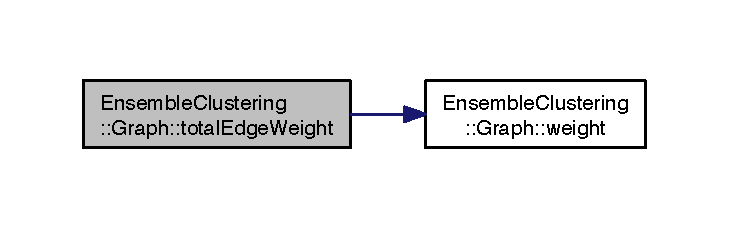
\includegraphics[width=350pt]{class_ensemble_clustering_1_1_graph_a7be7f13f5a31b0513293e7bbac26ca6c_cgraph}
\end{center}
\end{figure}


\hypertarget{class_ensemble_clustering_1_1_graph_a9bff231567f9ac604f1854d62f6682d1}{\index{Ensemble\-Clustering\-::\-Graph@{Ensemble\-Clustering\-::\-Graph}!weight@{weight}}
\index{weight@{weight}!EnsembleClustering::Graph@{Ensemble\-Clustering\-::\-Graph}}
\subsubsection[{weight}]{\setlength{\rightskip}{0pt plus 5cm}double Ensemble\-Clustering\-::\-Graph\-::weight (
\begin{DoxyParamCaption}
\item[{{\bf node}}]{v}
\end{DoxyParamCaption}
) const}}\label{class_ensemble_clustering_1_1_graph_a9bff231567f9ac604f1854d62f6682d1}


Return node weight. 



Definition at line 43 of file Graph.\-cpp.

\hypertarget{class_ensemble_clustering_1_1_graph_a656f5cb3119dd3f8f4182d38cce82fa0}{\index{Ensemble\-Clustering\-::\-Graph@{Ensemble\-Clustering\-::\-Graph}!weight@{weight}}
\index{weight@{weight}!EnsembleClustering::Graph@{Ensemble\-Clustering\-::\-Graph}}
\subsubsection[{weight}]{\setlength{\rightskip}{0pt plus 5cm}double Ensemble\-Clustering\-::\-Graph\-::weight (
\begin{DoxyParamCaption}
\item[{{\bf edge}}]{uv}
\end{DoxyParamCaption}
) const}}\label{class_ensemble_clustering_1_1_graph_a656f5cb3119dd3f8f4182d38cce82fa0}


Return edge weight. 



Definition at line 47 of file Graph.\-cpp.

\hypertarget{class_ensemble_clustering_1_1_graph_a4699131f4d3602ecda00eaf70a86cbea}{\index{Ensemble\-Clustering\-::\-Graph@{Ensemble\-Clustering\-::\-Graph}!weight@{weight}}
\index{weight@{weight}!EnsembleClustering::Graph@{Ensemble\-Clustering\-::\-Graph}}
\subsubsection[{weight}]{\setlength{\rightskip}{0pt plus 5cm}double Ensemble\-Clustering\-::\-Graph\-::weight (
\begin{DoxyParamCaption}
\item[{{\bf node}}]{u, }
\item[{{\bf node}}]{v}
\end{DoxyParamCaption}
) const\hspace{0.3cm}{\ttfamily [inline]}}}\label{class_ensemble_clustering_1_1_graph_a4699131f4d3602ecda00eaf70a86cbea}


Return edge weight. 

Equivalent to get\-Weight(edge uv) 

Definition at line 144 of file Graph.\-h.



\subsection{Member Data Documentation}
\hypertarget{class_ensemble_clustering_1_1_graph_a377621f37c1dc58f32ecec0fd229408e}{\index{Ensemble\-Clustering\-::\-Graph@{Ensemble\-Clustering\-::\-Graph}!default\-Edge\-Type@{default\-Edge\-Type}}
\index{default\-Edge\-Type@{default\-Edge\-Type}!EnsembleClustering::Graph@{Ensemble\-Clustering\-::\-Graph}}
\subsubsection[{default\-Edge\-Type}]{\setlength{\rightskip}{0pt plus 5cm}const int64\-\_\-t Ensemble\-Clustering\-::\-Graph\-::default\-Edge\-Type = 0\hspace{0.3cm}{\ttfamily [static]}}}\label{class_ensemble_clustering_1_1_graph_a377621f37c1dc58f32ecec0fd229408e}


Definition at line 92 of file Graph.\-h.

\hypertarget{class_ensemble_clustering_1_1_graph_a8186ee969064a4e12b779b1dc506ac60}{\index{Ensemble\-Clustering\-::\-Graph@{Ensemble\-Clustering\-::\-Graph}!default\-Edge\-Weight@{default\-Edge\-Weight}}
\index{default\-Edge\-Weight@{default\-Edge\-Weight}!EnsembleClustering::Graph@{Ensemble\-Clustering\-::\-Graph}}
\subsubsection[{default\-Edge\-Weight}]{\setlength{\rightskip}{0pt plus 5cm}constexpr double Ensemble\-Clustering\-::\-Graph\-::default\-Edge\-Weight = 1.\-0\hspace{0.3cm}{\ttfamily [static]}}}\label{class_ensemble_clustering_1_1_graph_a8186ee969064a4e12b779b1dc506ac60}


default parameters 



Definition at line 91 of file Graph.\-h.

\hypertarget{class_ensemble_clustering_1_1_graph_a9a6623d55f673a3b30e0c23284dd6da1}{\index{Ensemble\-Clustering\-::\-Graph@{Ensemble\-Clustering\-::\-Graph}!default\-Time\-Stamp@{default\-Time\-Stamp}}
\index{default\-Time\-Stamp@{default\-Time\-Stamp}!EnsembleClustering::Graph@{Ensemble\-Clustering\-::\-Graph}}
\subsubsection[{default\-Time\-Stamp}]{\setlength{\rightskip}{0pt plus 5cm}const int64\-\_\-t Ensemble\-Clustering\-::\-Graph\-::default\-Time\-Stamp = 0\hspace{0.3cm}{\ttfamily [static]}}}\label{class_ensemble_clustering_1_1_graph_a9a6623d55f673a3b30e0c23284dd6da1}


Definition at line 93 of file Graph.\-h.

\hypertarget{class_ensemble_clustering_1_1_graph_af83709e85afb91c70729405a725afb9a}{\index{Ensemble\-Clustering\-::\-Graph@{Ensemble\-Clustering\-::\-Graph}!stinger\-G@{stinger\-G}}
\index{stinger\-G@{stinger\-G}!EnsembleClustering::Graph@{Ensemble\-Clustering\-::\-Graph}}
\subsubsection[{stinger\-G}]{\setlength{\rightskip}{0pt plus 5cm}stinger$\ast$ Ensemble\-Clustering\-::\-Graph\-::stinger\-G\hspace{0.3cm}{\ttfamily [protected]}}}\label{class_ensemble_clustering_1_1_graph_af83709e85afb91c70729405a725afb9a}


Definition at line 81 of file Graph.\-h.



The documentation for this class was generated from the following files\-:\begin{DoxyCompactItemize}
\item 
src/graph/\hyperlink{_graph_8h}{Graph.\-h}\item 
src/graph/\hyperlink{_graph_8cpp}{Graph.\-cpp}\end{DoxyCompactItemize}

\hypertarget{class_ensemble_clustering_1_1_graph_generator}{\section{Ensemble\-Clustering\-:\-:Graph\-Generator Class Reference}
\label{class_ensemble_clustering_1_1_graph_generator}\index{Ensemble\-Clustering\-::\-Graph\-Generator@{Ensemble\-Clustering\-::\-Graph\-Generator}}
}


{\ttfamily \#include $<$Graph\-Generator.\-h$>$}

\subsection*{Public Member Functions}
\begin{DoxyCompactItemize}
\item 
\hyperlink{class_ensemble_clustering_1_1_graph_generator_a076eb95e34e465a0639844e79c79c4b0}{Graph\-Generator} ()
\item 
virtual \hyperlink{class_ensemble_clustering_1_1_graph_generator_a4f0b5374c64c6c81bf64e88a9b74b646}{$\sim$\-Graph\-Generator} ()
\item 
virtual \hyperlink{class_ensemble_clustering_1_1_graph}{Graph} \hyperlink{class_ensemble_clustering_1_1_graph_generator_ae3f01707491ceca4cdc6b87af45370ae}{make\-Erdos\-Renyi\-Graph} (\hyperlink{namespace_ensemble_clustering_a2482e94ca22a0c6544a5a9173186fde8}{count} n, double p)
\begin{DoxyCompactList}\small\item\em Generate a random graph according to the Erdos-\/\-Renyi model. \end{DoxyCompactList}\item 
virtual \hyperlink{class_ensemble_clustering_1_1_graph}{Graph} \hyperlink{class_ensemble_clustering_1_1_graph_generator_aec7e3e94b6e925077f7531da793a47a5}{make\-Random\-Graph} (\hyperlink{namespace_ensemble_clustering_a2482e94ca22a0c6544a5a9173186fde8}{count} n, double p)
\begin{DoxyCompactList}\small\item\em Alias for make\-Erdos\-Renyi\-Graph. \end{DoxyCompactList}\item 
virtual \hyperlink{class_ensemble_clustering_1_1_graph}{Graph} \hyperlink{class_ensemble_clustering_1_1_graph_generator_a6b1dfcef57d42bb6bccf2d15ea0aeac1}{make\-Circular\-Graph} (\hyperlink{namespace_ensemble_clustering_a2482e94ca22a0c6544a5a9173186fde8}{count} n)
\begin{DoxyCompactList}\small\item\em Generate a graph whose nodes and edges form a circle. \end{DoxyCompactList}\item 
virtual \hyperlink{class_ensemble_clustering_1_1_graph}{Graph} \hyperlink{class_ensemble_clustering_1_1_graph_generator_af418835f00a4fc70a76eebe7c70104d2}{make\-Complete\-Graph} (\hyperlink{namespace_ensemble_clustering_a2482e94ca22a0c6544a5a9173186fde8}{count} n)
\begin{DoxyCompactList}\small\item\em Generate a complete graph. \end{DoxyCompactList}\item 
virtual \hyperlink{class_ensemble_clustering_1_1_graph}{Graph} \hyperlink{class_ensemble_clustering_1_1_graph_generator_aefc6fbc6e23235419d1a2030d688b4bd}{make\-Clustered\-Random\-Graph} (\hyperlink{namespace_ensemble_clustering_a2482e94ca22a0c6544a5a9173186fde8}{count} n, \hyperlink{namespace_ensemble_clustering_a2482e94ca22a0c6544a5a9173186fde8}{count} k, double pin, double pout)
\begin{DoxyCompactList}\small\item\em Creates a clustered random graph\-: \end{DoxyCompactList}\item 
virtual std\-::pair$<$ \hyperlink{class_ensemble_clustering_1_1_graph}{Graph}, \\*
\hyperlink{class_ensemble_clustering_1_1_clustering}{Clustering} $>$ \hyperlink{class_ensemble_clustering_1_1_graph_generator_a573c023203806f719bdd0caf17764340}{make\-Clustered\-Random\-Graph\-With\-Reference\-Clustering} (\hyperlink{namespace_ensemble_clustering_a2482e94ca22a0c6544a5a9173186fde8}{count} n, \hyperlink{namespace_ensemble_clustering_a2482e94ca22a0c6544a5a9173186fde8}{count} k, double pin, double pout)
\begin{DoxyCompactList}\small\item\em Creates a clustered random graph\-: \end{DoxyCompactList}\item 
virtual \hyperlink{class_ensemble_clustering_1_1_graph}{Graph} \hyperlink{class_ensemble_clustering_1_1_graph_generator_a098d0364dc2792e97f7242f5df1534d0}{make\-Clustered\-Random\-Graph} (\hyperlink{class_ensemble_clustering_1_1_clustering}{Clustering} \&zeta, double pin, double pout)
\begin{DoxyCompactList}\small\item\em Create a clustered random graph from a given clustering. \end{DoxyCompactList}\item 
virtual \hyperlink{class_ensemble_clustering_1_1_graph}{Graph} \hyperlink{class_ensemble_clustering_1_1_graph_generator_aca4bcf582579a571c5a6b4a1cd59770e}{make\-Preferential\-Attachment\-Graph} (\hyperlink{namespace_ensemble_clustering_a2482e94ca22a0c6544a5a9173186fde8}{count} n, \hyperlink{namespace_ensemble_clustering_a2482e94ca22a0c6544a5a9173186fde8}{count} a)
\begin{DoxyCompactList}\small\item\em Generate random graph according to the Barabasi-\/\-Albert model (preferential attachment) \end{DoxyCompactList}\end{DoxyCompactItemize}


\subsection{Detailed Description}


Definition at line 18 of file Graph\-Generator.\-h.



\subsection{Constructor \& Destructor Documentation}
\hypertarget{class_ensemble_clustering_1_1_graph_generator_a076eb95e34e465a0639844e79c79c4b0}{\index{Ensemble\-Clustering\-::\-Graph\-Generator@{Ensemble\-Clustering\-::\-Graph\-Generator}!Graph\-Generator@{Graph\-Generator}}
\index{Graph\-Generator@{Graph\-Generator}!EnsembleClustering::GraphGenerator@{Ensemble\-Clustering\-::\-Graph\-Generator}}
\subsubsection[{Graph\-Generator}]{\setlength{\rightskip}{0pt plus 5cm}Ensemble\-Clustering\-::\-Graph\-Generator\-::\-Graph\-Generator (
\begin{DoxyParamCaption}
{}
\end{DoxyParamCaption}
)}}\label{class_ensemble_clustering_1_1_graph_generator_a076eb95e34e465a0639844e79c79c4b0}


Definition at line 12 of file Graph\-Generator.\-cpp.

\hypertarget{class_ensemble_clustering_1_1_graph_generator_a4f0b5374c64c6c81bf64e88a9b74b646}{\index{Ensemble\-Clustering\-::\-Graph\-Generator@{Ensemble\-Clustering\-::\-Graph\-Generator}!$\sim$\-Graph\-Generator@{$\sim$\-Graph\-Generator}}
\index{$\sim$\-Graph\-Generator@{$\sim$\-Graph\-Generator}!EnsembleClustering::GraphGenerator@{Ensemble\-Clustering\-::\-Graph\-Generator}}
\subsubsection[{$\sim$\-Graph\-Generator}]{\setlength{\rightskip}{0pt plus 5cm}Ensemble\-Clustering\-::\-Graph\-Generator\-::$\sim$\-Graph\-Generator (
\begin{DoxyParamCaption}
{}
\end{DoxyParamCaption}
)\hspace{0.3cm}{\ttfamily [virtual]}}}\label{class_ensemble_clustering_1_1_graph_generator_a4f0b5374c64c6c81bf64e88a9b74b646}


Definition at line 17 of file Graph\-Generator.\-cpp.



\subsection{Member Function Documentation}
\hypertarget{class_ensemble_clustering_1_1_graph_generator_a6b1dfcef57d42bb6bccf2d15ea0aeac1}{\index{Ensemble\-Clustering\-::\-Graph\-Generator@{Ensemble\-Clustering\-::\-Graph\-Generator}!make\-Circular\-Graph@{make\-Circular\-Graph}}
\index{make\-Circular\-Graph@{make\-Circular\-Graph}!EnsembleClustering::GraphGenerator@{Ensemble\-Clustering\-::\-Graph\-Generator}}
\subsubsection[{make\-Circular\-Graph}]{\setlength{\rightskip}{0pt plus 5cm}{\bf Graph} Ensemble\-Clustering\-::\-Graph\-Generator\-::make\-Circular\-Graph (
\begin{DoxyParamCaption}
\item[{{\bf count}}]{n}
\end{DoxyParamCaption}
)\hspace{0.3cm}{\ttfamily [virtual]}}}\label{class_ensemble_clustering_1_1_graph_generator_a6b1dfcef57d42bb6bccf2d15ea0aeac1}


Generate a graph whose nodes and edges form a circle. 


\begin{DoxyParams}[1]{Parameters}
\mbox{\tt in}  & {\em n} & number of nodes \\
\hline
\end{DoxyParams}


Definition at line 41 of file Graph\-Generator.\-cpp.



Here is the call graph for this function\-:
\nopagebreak
\begin{figure}[H]
\begin{center}
\leavevmode
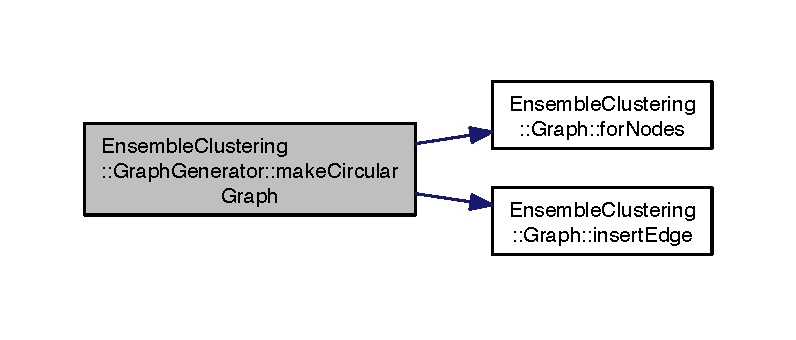
\includegraphics[width=350pt]{class_ensemble_clustering_1_1_graph_generator_a6b1dfcef57d42bb6bccf2d15ea0aeac1_cgraph}
\end{center}
\end{figure}


\hypertarget{class_ensemble_clustering_1_1_graph_generator_aefc6fbc6e23235419d1a2030d688b4bd}{\index{Ensemble\-Clustering\-::\-Graph\-Generator@{Ensemble\-Clustering\-::\-Graph\-Generator}!make\-Clustered\-Random\-Graph@{make\-Clustered\-Random\-Graph}}
\index{make\-Clustered\-Random\-Graph@{make\-Clustered\-Random\-Graph}!EnsembleClustering::GraphGenerator@{Ensemble\-Clustering\-::\-Graph\-Generator}}
\subsubsection[{make\-Clustered\-Random\-Graph}]{\setlength{\rightskip}{0pt plus 5cm}{\bf Graph} Ensemble\-Clustering\-::\-Graph\-Generator\-::make\-Clustered\-Random\-Graph (
\begin{DoxyParamCaption}
\item[{{\bf count}}]{n, }
\item[{{\bf count}}]{k, }
\item[{double}]{pin, }
\item[{double}]{pout}
\end{DoxyParamCaption}
)\hspace{0.3cm}{\ttfamily [virtual]}}}\label{class_ensemble_clustering_1_1_graph_generator_aefc6fbc6e23235419d1a2030d688b4bd}


Creates a clustered random graph\-: 


\begin{DoxyParams}[1]{Parameters}
\mbox{\tt in}  & {\em n} & number of nodes \\
\hline
\mbox{\tt in}  & {\em k} & number of clusters \\
\hline
\mbox{\tt in}  & {\em pin} & intra-\/cluster edge probability \\
\hline
\mbox{\tt in}  & {\em pout} & inter-\/cluster edge probability \\
\hline
\end{DoxyParams}


Definition at line 62 of file Graph\-Generator.\-cpp.



Here is the call graph for this function\-:
\nopagebreak
\begin{figure}[H]
\begin{center}
\leavevmode
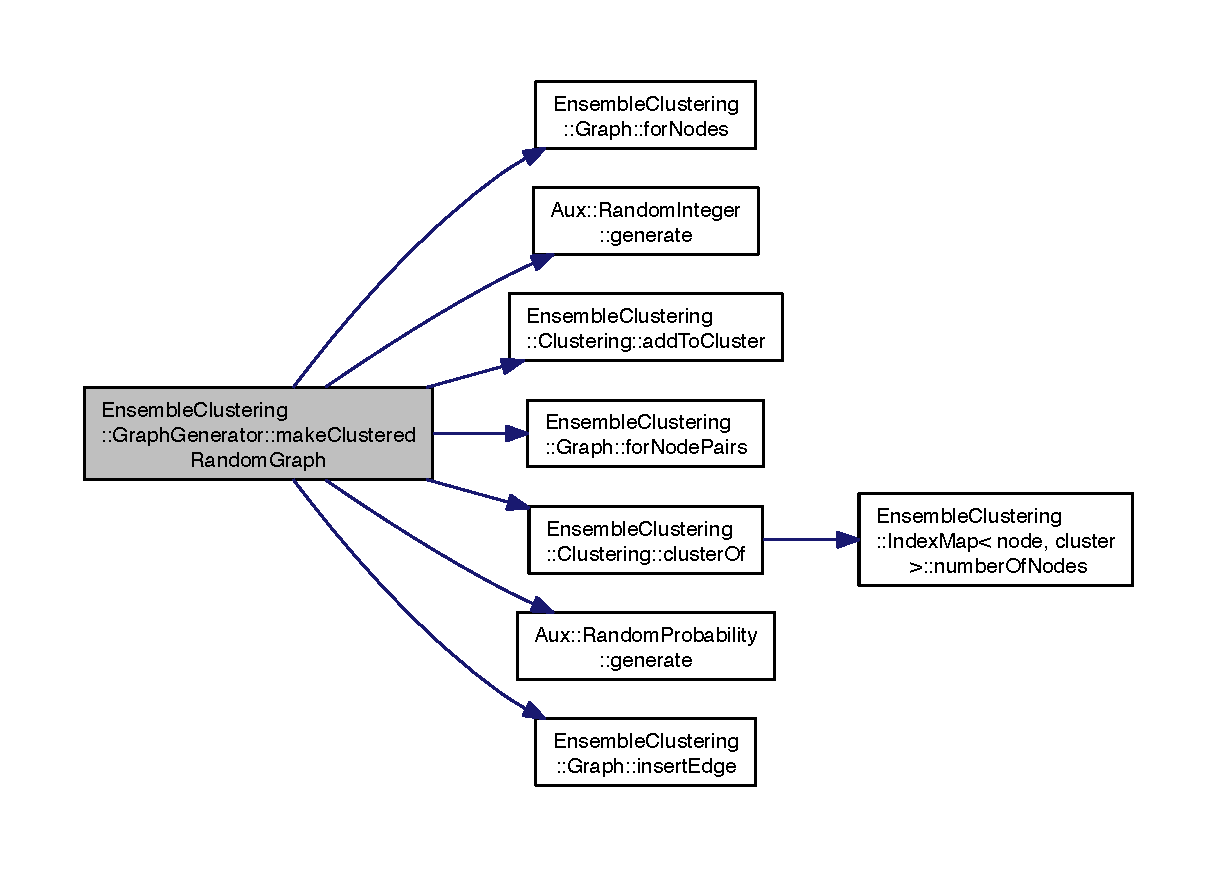
\includegraphics[width=350pt]{class_ensemble_clustering_1_1_graph_generator_aefc6fbc6e23235419d1a2030d688b4bd_cgraph}
\end{center}
\end{figure}


\hypertarget{class_ensemble_clustering_1_1_graph_generator_a098d0364dc2792e97f7242f5df1534d0}{\index{Ensemble\-Clustering\-::\-Graph\-Generator@{Ensemble\-Clustering\-::\-Graph\-Generator}!make\-Clustered\-Random\-Graph@{make\-Clustered\-Random\-Graph}}
\index{make\-Clustered\-Random\-Graph@{make\-Clustered\-Random\-Graph}!EnsembleClustering::GraphGenerator@{Ensemble\-Clustering\-::\-Graph\-Generator}}
\subsubsection[{make\-Clustered\-Random\-Graph}]{\setlength{\rightskip}{0pt plus 5cm}{\bf Graph} Ensemble\-Clustering\-::\-Graph\-Generator\-::make\-Clustered\-Random\-Graph (
\begin{DoxyParamCaption}
\item[{{\bf Clustering} \&}]{zeta, }
\item[{double}]{pin, }
\item[{double}]{pout}
\end{DoxyParamCaption}
)\hspace{0.3cm}{\ttfamily [virtual]}}}\label{class_ensemble_clustering_1_1_graph_generator_a098d0364dc2792e97f7242f5df1534d0}


Create a clustered random graph from a given clustering. 



Definition at line 121 of file Graph\-Generator.\-cpp.



Here is the call graph for this function\-:
\nopagebreak
\begin{figure}[H]
\begin{center}
\leavevmode
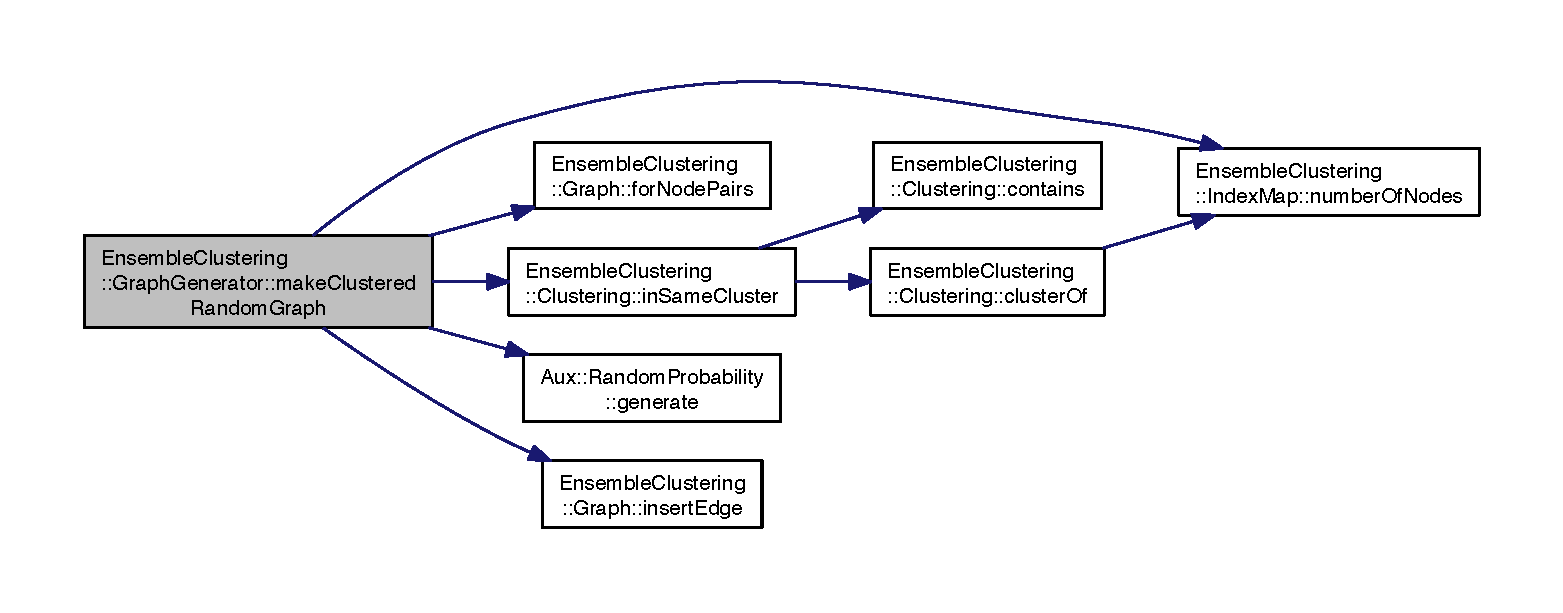
\includegraphics[width=350pt]{class_ensemble_clustering_1_1_graph_generator_a098d0364dc2792e97f7242f5df1534d0_cgraph}
\end{center}
\end{figure}


\hypertarget{class_ensemble_clustering_1_1_graph_generator_a573c023203806f719bdd0caf17764340}{\index{Ensemble\-Clustering\-::\-Graph\-Generator@{Ensemble\-Clustering\-::\-Graph\-Generator}!make\-Clustered\-Random\-Graph\-With\-Reference\-Clustering@{make\-Clustered\-Random\-Graph\-With\-Reference\-Clustering}}
\index{make\-Clustered\-Random\-Graph\-With\-Reference\-Clustering@{make\-Clustered\-Random\-Graph\-With\-Reference\-Clustering}!EnsembleClustering::GraphGenerator@{Ensemble\-Clustering\-::\-Graph\-Generator}}
\subsubsection[{make\-Clustered\-Random\-Graph\-With\-Reference\-Clustering}]{\setlength{\rightskip}{0pt plus 5cm}std\-::pair$<$ {\bf Graph}, {\bf Clustering} $>$ Ensemble\-Clustering\-::\-Graph\-Generator\-::make\-Clustered\-Random\-Graph\-With\-Reference\-Clustering (
\begin{DoxyParamCaption}
\item[{{\bf count}}]{n, }
\item[{{\bf count}}]{k, }
\item[{double}]{pin, }
\item[{double}]{pout}
\end{DoxyParamCaption}
)\hspace{0.3cm}{\ttfamily [virtual]}}}\label{class_ensemble_clustering_1_1_graph_generator_a573c023203806f719bdd0caf17764340}


Creates a clustered random graph\-: 


\begin{DoxyParams}[1]{Parameters}
\mbox{\tt in}  & {\em n} & number of nodes \\
\hline
\mbox{\tt in}  & {\em k} & number of clusters \\
\hline
\mbox{\tt in}  & {\em pin} & intra-\/cluster edge probability \\
\hline
\mbox{\tt in}  & {\em pout} & inter-\/cluster edge probability \\
\hline
\end{DoxyParams}


Definition at line 92 of file Graph\-Generator.\-cpp.



Here is the call graph for this function\-:
\nopagebreak
\begin{figure}[H]
\begin{center}
\leavevmode
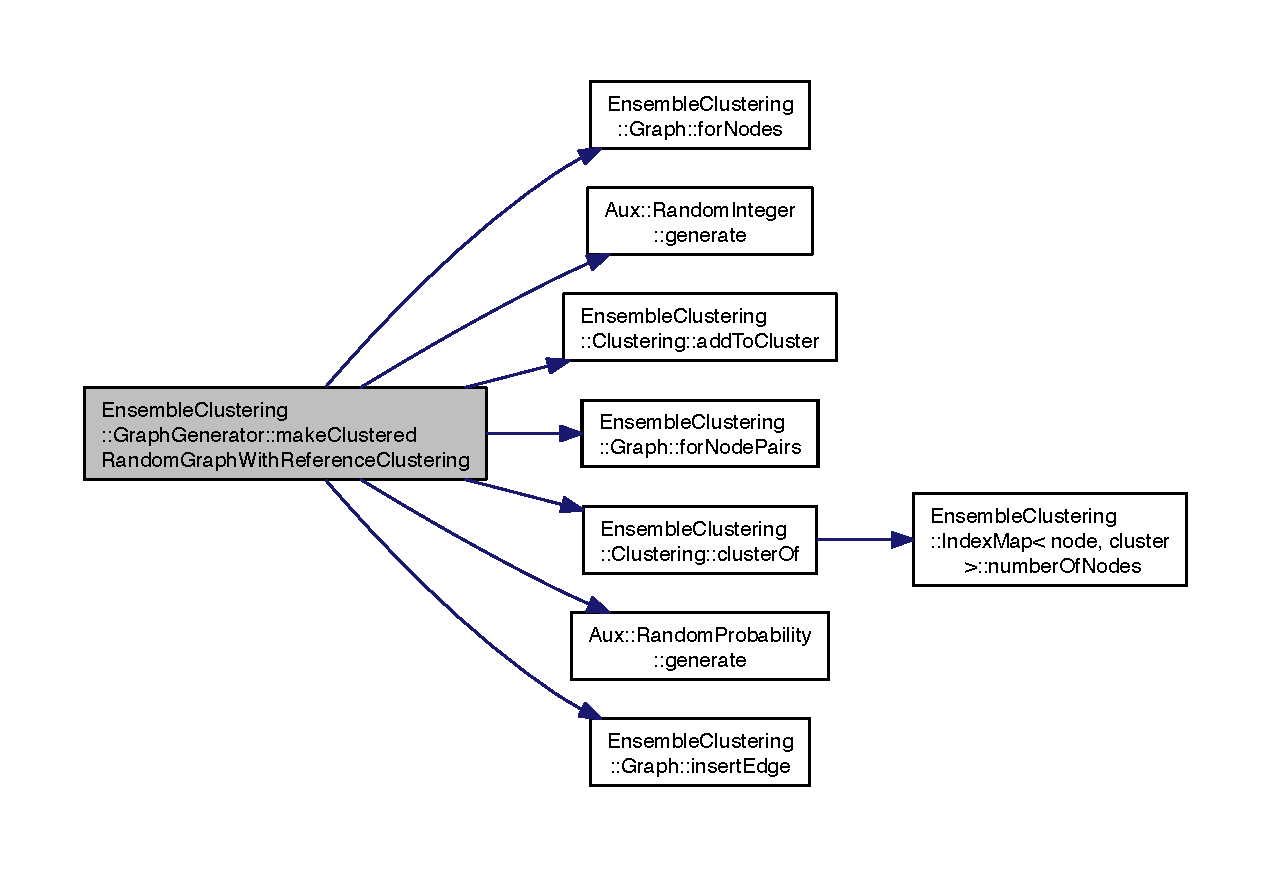
\includegraphics[width=350pt]{class_ensemble_clustering_1_1_graph_generator_a573c023203806f719bdd0caf17764340_cgraph}
\end{center}
\end{figure}


\hypertarget{class_ensemble_clustering_1_1_graph_generator_af418835f00a4fc70a76eebe7c70104d2}{\index{Ensemble\-Clustering\-::\-Graph\-Generator@{Ensemble\-Clustering\-::\-Graph\-Generator}!make\-Complete\-Graph@{make\-Complete\-Graph}}
\index{make\-Complete\-Graph@{make\-Complete\-Graph}!EnsembleClustering::GraphGenerator@{Ensemble\-Clustering\-::\-Graph\-Generator}}
\subsubsection[{make\-Complete\-Graph}]{\setlength{\rightskip}{0pt plus 5cm}{\bf Graph} Ensemble\-Clustering\-::\-Graph\-Generator\-::make\-Complete\-Graph (
\begin{DoxyParamCaption}
\item[{{\bf count}}]{n}
\end{DoxyParamCaption}
)\hspace{0.3cm}{\ttfamily [virtual]}}}\label{class_ensemble_clustering_1_1_graph_generator_af418835f00a4fc70a76eebe7c70104d2}


Generate a complete graph. 


\begin{DoxyParams}[1]{Parameters}
\mbox{\tt in}  & {\em n} & number of nodes \\
\hline
\end{DoxyParams}


Definition at line 50 of file Graph\-Generator.\-cpp.



Here is the call graph for this function\-:
\nopagebreak
\begin{figure}[H]
\begin{center}
\leavevmode
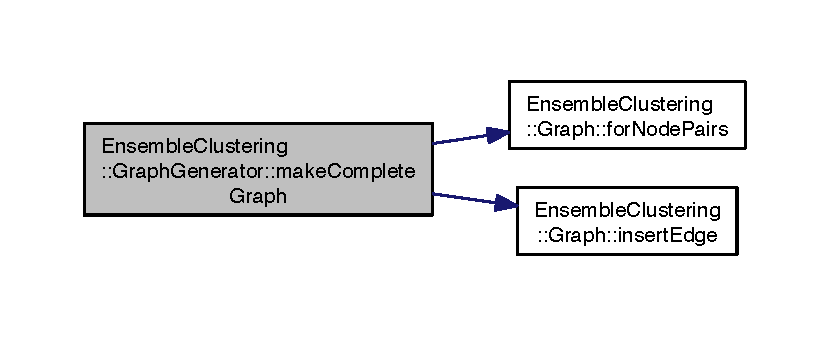
\includegraphics[width=350pt]{class_ensemble_clustering_1_1_graph_generator_af418835f00a4fc70a76eebe7c70104d2_cgraph}
\end{center}
\end{figure}


\hypertarget{class_ensemble_clustering_1_1_graph_generator_ae3f01707491ceca4cdc6b87af45370ae}{\index{Ensemble\-Clustering\-::\-Graph\-Generator@{Ensemble\-Clustering\-::\-Graph\-Generator}!make\-Erdos\-Renyi\-Graph@{make\-Erdos\-Renyi\-Graph}}
\index{make\-Erdos\-Renyi\-Graph@{make\-Erdos\-Renyi\-Graph}!EnsembleClustering::GraphGenerator@{Ensemble\-Clustering\-::\-Graph\-Generator}}
\subsubsection[{make\-Erdos\-Renyi\-Graph}]{\setlength{\rightskip}{0pt plus 5cm}{\bf Graph} Ensemble\-Clustering\-::\-Graph\-Generator\-::make\-Erdos\-Renyi\-Graph (
\begin{DoxyParamCaption}
\item[{{\bf count}}]{n, }
\item[{double}]{p}
\end{DoxyParamCaption}
)\hspace{0.3cm}{\ttfamily [virtual]}}}\label{class_ensemble_clustering_1_1_graph_generator_ae3f01707491ceca4cdc6b87af45370ae}


Generate a random graph according to the Erdos-\/\-Renyi model. 


\begin{DoxyParams}[1]{Parameters}
\mbox{\tt in}  & {\em n} & number of nodes \\
\hline
\mbox{\tt in}  & {\em p} & edge probability \\
\hline
\end{DoxyParams}


Definition at line 25 of file Graph\-Generator.\-cpp.



Here is the call graph for this function\-:
\nopagebreak
\begin{figure}[H]
\begin{center}
\leavevmode
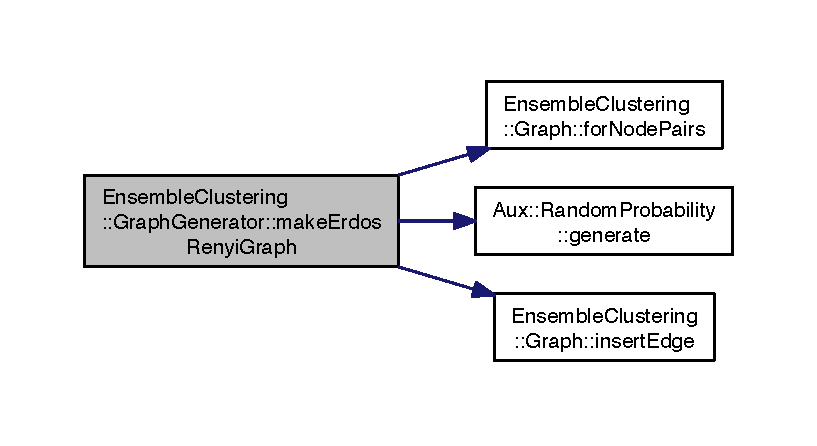
\includegraphics[width=350pt]{class_ensemble_clustering_1_1_graph_generator_ae3f01707491ceca4cdc6b87af45370ae_cgraph}
\end{center}
\end{figure}


\hypertarget{class_ensemble_clustering_1_1_graph_generator_aca4bcf582579a571c5a6b4a1cd59770e}{\index{Ensemble\-Clustering\-::\-Graph\-Generator@{Ensemble\-Clustering\-::\-Graph\-Generator}!make\-Preferential\-Attachment\-Graph@{make\-Preferential\-Attachment\-Graph}}
\index{make\-Preferential\-Attachment\-Graph@{make\-Preferential\-Attachment\-Graph}!EnsembleClustering::GraphGenerator@{Ensemble\-Clustering\-::\-Graph\-Generator}}
\subsubsection[{make\-Preferential\-Attachment\-Graph}]{\setlength{\rightskip}{0pt plus 5cm}{\bf Graph} Ensemble\-Clustering\-::\-Graph\-Generator\-::make\-Preferential\-Attachment\-Graph (
\begin{DoxyParamCaption}
\item[{{\bf count}}]{n, }
\item[{{\bf count}}]{a}
\end{DoxyParamCaption}
)\hspace{0.3cm}{\ttfamily [virtual]}}}\label{class_ensemble_clustering_1_1_graph_generator_aca4bcf582579a571c5a6b4a1cd59770e}


Generate random graph according to the Barabasi-\/\-Albert model (preferential attachment) 


\begin{DoxyParams}[1]{Parameters}
\mbox{\tt in}  & {\em n} & number of nodes \\
\hline
\mbox{\tt in}  & {\em a} & number of edges added for each node \\
\hline
\end{DoxyParams}


Definition at line 144 of file Graph\-Generator.\-cpp.



Here is the call graph for this function\-:
\nopagebreak
\begin{figure}[H]
\begin{center}
\leavevmode
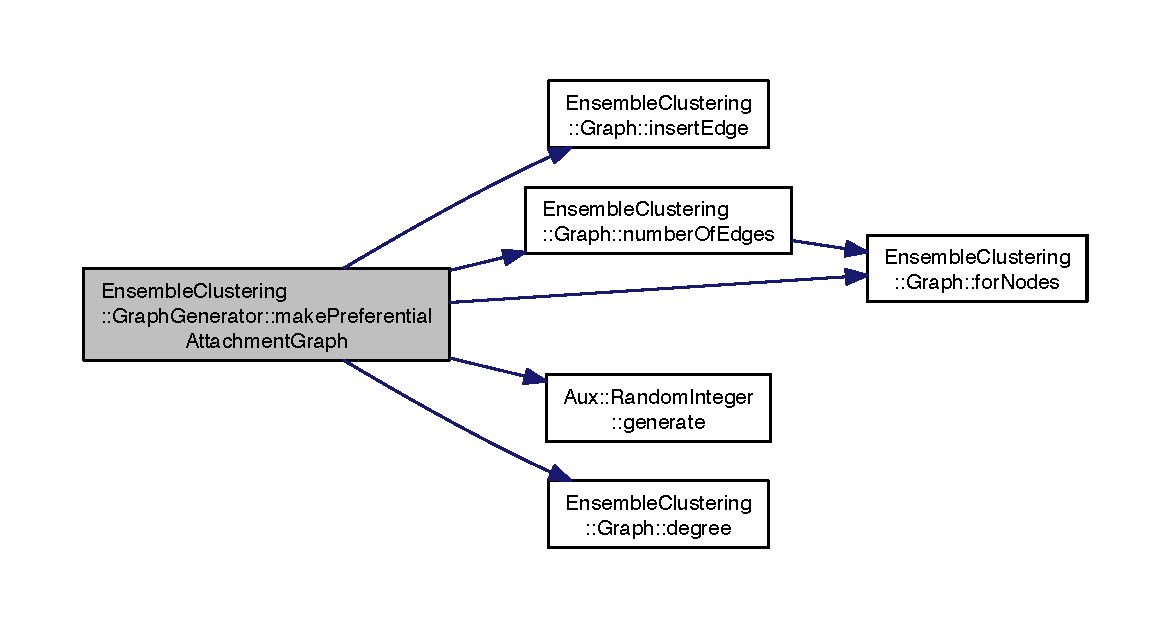
\includegraphics[width=350pt]{class_ensemble_clustering_1_1_graph_generator_aca4bcf582579a571c5a6b4a1cd59770e_cgraph}
\end{center}
\end{figure}


\hypertarget{class_ensemble_clustering_1_1_graph_generator_aec7e3e94b6e925077f7531da793a47a5}{\index{Ensemble\-Clustering\-::\-Graph\-Generator@{Ensemble\-Clustering\-::\-Graph\-Generator}!make\-Random\-Graph@{make\-Random\-Graph}}
\index{make\-Random\-Graph@{make\-Random\-Graph}!EnsembleClustering::GraphGenerator@{Ensemble\-Clustering\-::\-Graph\-Generator}}
\subsubsection[{make\-Random\-Graph}]{\setlength{\rightskip}{0pt plus 5cm}{\bf Graph} Ensemble\-Clustering\-::\-Graph\-Generator\-::make\-Random\-Graph (
\begin{DoxyParamCaption}
\item[{{\bf count}}]{n, }
\item[{double}]{p}
\end{DoxyParamCaption}
)\hspace{0.3cm}{\ttfamily [virtual]}}}\label{class_ensemble_clustering_1_1_graph_generator_aec7e3e94b6e925077f7531da793a47a5}


Alias for make\-Erdos\-Renyi\-Graph. 



Definition at line 37 of file Graph\-Generator.\-cpp.



Here is the call graph for this function\-:
\nopagebreak
\begin{figure}[H]
\begin{center}
\leavevmode
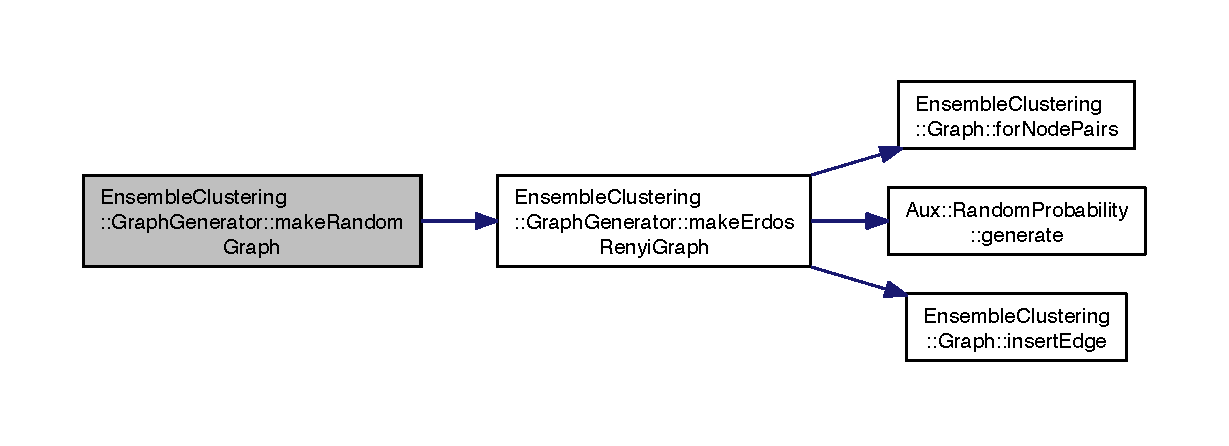
\includegraphics[width=350pt]{class_ensemble_clustering_1_1_graph_generator_aec7e3e94b6e925077f7531da793a47a5_cgraph}
\end{center}
\end{figure}




The documentation for this class was generated from the following files\-:\begin{DoxyCompactItemize}
\item 
src/graph/\hyperlink{_graph_generator_8h}{Graph\-Generator.\-h}\item 
src/graph/\hyperlink{_graph_generator_8cpp}{Graph\-Generator.\-cpp}\end{DoxyCompactItemize}

\hypertarget{class_ensemble_clustering_1_1_graph_g_test}{\section{Ensemble\-Clustering\-:\-:Graph\-G\-Test Class Reference}
\label{class_ensemble_clustering_1_1_graph_g_test}\index{Ensemble\-Clustering\-::\-Graph\-G\-Test@{Ensemble\-Clustering\-::\-Graph\-G\-Test}}
}


{\ttfamily \#include $<$Graph\-G\-Test.\-h$>$}



Inheritance diagram for Ensemble\-Clustering\-:\-:Graph\-G\-Test\-:\nopagebreak
\begin{figure}[H]
\begin{center}
\leavevmode
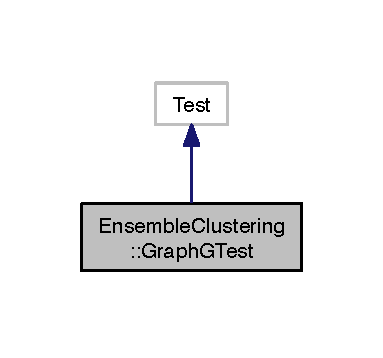
\includegraphics[width=184pt]{class_ensemble_clustering_1_1_graph_g_test__inherit__graph}
\end{center}
\end{figure}


Collaboration diagram for Ensemble\-Clustering\-:\-:Graph\-G\-Test\-:\nopagebreak
\begin{figure}[H]
\begin{center}
\leavevmode
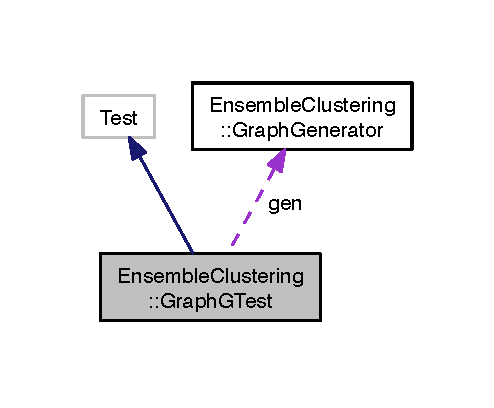
\includegraphics[width=237pt]{class_ensemble_clustering_1_1_graph_g_test__coll__graph}
\end{center}
\end{figure}
\subsection*{Public Member Functions}
\begin{DoxyCompactItemize}
\item 
virtual void \hyperlink{class_ensemble_clustering_1_1_graph_g_test_ae9469ed9c84ebaaefe10dbe444209ee7}{Set\-Up} ()
\item 
virtual void \hyperlink{class_ensemble_clustering_1_1_graph_g_test_a32e82eb324570ff482a870c3c3a43899}{Tear\-Down} ()
\end{DoxyCompactItemize}
\subsection*{Protected Attributes}
\begin{DoxyCompactItemize}
\item 
\hyperlink{class_ensemble_clustering_1_1_graph_generator}{Graph\-Generator} \hyperlink{class_ensemble_clustering_1_1_graph_g_test_a8233040cfa6b04e5a36d2bc0bfe1bc07}{gen}
\end{DoxyCompactItemize}


\subsection{Detailed Description}


Definition at line 20 of file Graph\-G\-Test.\-h.



\subsection{Member Function Documentation}
\hypertarget{class_ensemble_clustering_1_1_graph_g_test_ae9469ed9c84ebaaefe10dbe444209ee7}{\index{Ensemble\-Clustering\-::\-Graph\-G\-Test@{Ensemble\-Clustering\-::\-Graph\-G\-Test}!Set\-Up@{Set\-Up}}
\index{Set\-Up@{Set\-Up}!EnsembleClustering::GraphGTest@{Ensemble\-Clustering\-::\-Graph\-G\-Test}}
\subsubsection[{Set\-Up}]{\setlength{\rightskip}{0pt plus 5cm}void Ensemble\-Clustering\-::\-Graph\-G\-Test\-::\-Set\-Up (
\begin{DoxyParamCaption}
{}
\end{DoxyParamCaption}
)\hspace{0.3cm}{\ttfamily [virtual]}}}\label{class_ensemble_clustering_1_1_graph_g_test_ae9469ed9c84ebaaefe10dbe444209ee7}


Definition at line 255 of file Graph\-G\-Test.\-cpp.

\hypertarget{class_ensemble_clustering_1_1_graph_g_test_a32e82eb324570ff482a870c3c3a43899}{\index{Ensemble\-Clustering\-::\-Graph\-G\-Test@{Ensemble\-Clustering\-::\-Graph\-G\-Test}!Tear\-Down@{Tear\-Down}}
\index{Tear\-Down@{Tear\-Down}!EnsembleClustering::GraphGTest@{Ensemble\-Clustering\-::\-Graph\-G\-Test}}
\subsubsection[{Tear\-Down}]{\setlength{\rightskip}{0pt plus 5cm}void Ensemble\-Clustering\-::\-Graph\-G\-Test\-::\-Tear\-Down (
\begin{DoxyParamCaption}
{}
\end{DoxyParamCaption}
)\hspace{0.3cm}{\ttfamily [virtual]}}}\label{class_ensemble_clustering_1_1_graph_g_test_a32e82eb324570ff482a870c3c3a43899}


Definition at line 258 of file Graph\-G\-Test.\-cpp.



\subsection{Member Data Documentation}
\hypertarget{class_ensemble_clustering_1_1_graph_g_test_a8233040cfa6b04e5a36d2bc0bfe1bc07}{\index{Ensemble\-Clustering\-::\-Graph\-G\-Test@{Ensemble\-Clustering\-::\-Graph\-G\-Test}!gen@{gen}}
\index{gen@{gen}!EnsembleClustering::GraphGTest@{Ensemble\-Clustering\-::\-Graph\-G\-Test}}
\subsubsection[{gen}]{\setlength{\rightskip}{0pt plus 5cm}{\bf Graph\-Generator} Ensemble\-Clustering\-::\-Graph\-G\-Test\-::gen\hspace{0.3cm}{\ttfamily [protected]}}}\label{class_ensemble_clustering_1_1_graph_g_test_a8233040cfa6b04e5a36d2bc0bfe1bc07}


Definition at line 24 of file Graph\-G\-Test.\-h.



The documentation for this class was generated from the following files\-:\begin{DoxyCompactItemize}
\item 
src/graph/test/\hyperlink{_graph_g_test_8h}{Graph\-G\-Test.\-h}\item 
src/graph/test/\hyperlink{_graph_g_test_8cpp}{Graph\-G\-Test.\-cpp}\end{DoxyCompactItemize}

\hypertarget{class_g_test_test}{\section{G\-Test\-Test Class Reference}
\label{class_g_test_test}\index{G\-Test\-Test@{G\-Test\-Test}}
}


{\ttfamily \#include $<$Test\-G\-Test.\-h$>$}



Inheritance diagram for G\-Test\-Test\-:\nopagebreak
\begin{figure}[H]
\begin{center}
\leavevmode
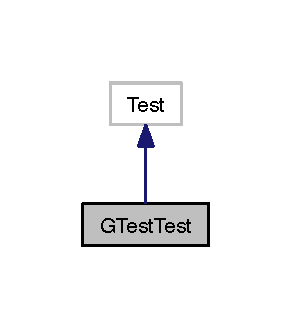
\includegraphics[width=140pt]{class_g_test_test__inherit__graph}
\end{center}
\end{figure}


Collaboration diagram for G\-Test\-Test\-:\nopagebreak
\begin{figure}[H]
\begin{center}
\leavevmode
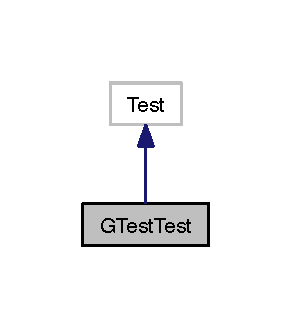
\includegraphics[width=140pt]{class_g_test_test__coll__graph}
\end{center}
\end{figure}
\subsection*{Protected Member Functions}
\begin{DoxyCompactItemize}
\item 
virtual void \hyperlink{class_g_test_test_ac1d7b693d1ce5ab93890720bed6e8d29}{Set\-Up} ()
\end{DoxyCompactItemize}


\subsection{Detailed Description}


Definition at line 13 of file Test\-G\-Test.\-h.



\subsection{Member Function Documentation}
\hypertarget{class_g_test_test_ac1d7b693d1ce5ab93890720bed6e8d29}{\index{G\-Test\-Test@{G\-Test\-Test}!Set\-Up@{Set\-Up}}
\index{Set\-Up@{Set\-Up}!GTestTest@{G\-Test\-Test}}
\subsubsection[{Set\-Up}]{\setlength{\rightskip}{0pt plus 5cm}virtual void G\-Test\-Test\-::\-Set\-Up (
\begin{DoxyParamCaption}
{}
\end{DoxyParamCaption}
)\hspace{0.3cm}{\ttfamily [inline]}, {\ttfamily [protected]}, {\ttfamily [virtual]}}}\label{class_g_test_test_ac1d7b693d1ce5ab93890720bed6e8d29}


Definition at line 16 of file Test\-G\-Test.\-h.



The documentation for this class was generated from the following file\-:\begin{DoxyCompactItemize}
\item 
src/test/\hyperlink{_test_g_test_8h}{Test\-G\-Test.\-h}\end{DoxyCompactItemize}

\hypertarget{class_ensemble_clustering_1_1_index_map}{\section{Ensemble\-Clustering\-:\-:Index\-Map$<$ I, T $>$ Class Template Reference}
\label{class_ensemble_clustering_1_1_index_map}\index{Ensemble\-Clustering\-::\-Index\-Map$<$ I, T $>$@{Ensemble\-Clustering\-::\-Index\-Map$<$ I, T $>$}}
}


An \hyperlink{class_ensemble_clustering_1_1_index_map}{Index\-Map} implements a 0-\/based mapping from an integer index type to an arbitray value type.  




{\ttfamily \#include $<$Index\-Map.\-h$>$}



Collaboration diagram for Ensemble\-Clustering\-:\-:Index\-Map$<$ I, T $>$\-:\nopagebreak
\begin{figure}[H]
\begin{center}
\leavevmode
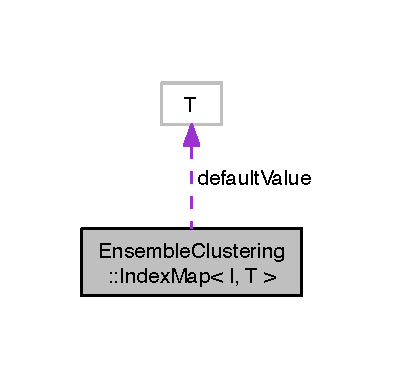
\includegraphics[width=190pt]{class_ensemble_clustering_1_1_index_map__coll__graph}
\end{center}
\end{figure}
\subsection*{Public Member Functions}
\begin{DoxyCompactItemize}
\item 
\hyperlink{class_ensemble_clustering_1_1_index_map_a475e833d787f15cb3ea392d2a986af3b}{Index\-Map} (int64\-\_\-t \hyperlink{class_ensemble_clustering_1_1_index_map_a3151d302c54e6ad0175bd87aef62d4ca}{n}, T \hyperlink{class_ensemble_clustering_1_1_index_map_ab5f1dc778237131e9d6c5713c2b318ec}{default\-Value})
\begin{DoxyCompactList}\small\item\em Construct a new \hyperlink{class_ensemble_clustering_1_1_index_map}{Index\-Map} which holds n entries . \end{DoxyCompactList}\item 
virtual \hyperlink{class_ensemble_clustering_1_1_index_map_aa4d08669a9bc3863b01f924c8d115328}{$\sim$\-Index\-Map} ()
\item 
T \& \hyperlink{class_ensemble_clustering_1_1_index_map_a961b55c469821e1a66cbdb1113a10f22}{operator\mbox{[}$\,$\mbox{]}} (const I \&\hyperlink{namespace_ensemble_clustering_a1ba11e6d628873b803a26fe054f45e28}{index})
\begin{DoxyCompactList}\small\item\em Index operator. \end{DoxyCompactList}\item 
const T \& \hyperlink{class_ensemble_clustering_1_1_index_map_afa664fe610c7cd8871125ba041bb9374}{operator\mbox{[}$\,$\mbox{]}} (const I \&\hyperlink{namespace_ensemble_clustering_a1ba11e6d628873b803a26fe054f45e28}{index}) const 
\begin{DoxyCompactList}\small\item\em Index operator for const instances of this class. \end{DoxyCompactList}\item 
virtual T \hyperlink{class_ensemble_clustering_1_1_index_map_ac3cb340d385ef58e348f16038017fc3a}{at} (I \hyperlink{namespace_ensemble_clustering_a1ba11e6d628873b803a26fe054f45e28}{index})
\item 
int64\-\_\-t \hyperlink{class_ensemble_clustering_1_1_index_map_a53354adcfc7081e8c3bc82e9f5c632a1}{number\-Of\-Entries} () const 
\begin{DoxyCompactList}\small\item\em Get the number of 1-\/based entries in this map. \end{DoxyCompactList}\item 
bool \hyperlink{class_ensemble_clustering_1_1_index_map_a059e36d3c7900f33daa397b0491dfdb6}{has\-Been\-Set} (I \hyperlink{namespace_ensemble_clustering_a1ba11e6d628873b803a26fe054f45e28}{index}) const 
\begin{DoxyCompactList}\small\item\em Check whether map contains an entry other than the default. \end{DoxyCompactList}\item 
virtual int64\-\_\-t \hyperlink{class_ensemble_clustering_1_1_index_map_a12dd2383d0014aefbc3b496998fa1383}{number\-Of\-Nodes} () const 
\begin{DoxyCompactList}\small\item\em Number of nodes for which this clsutering can hold an entry. \end{DoxyCompactList}\item 
virtual void \hyperlink{class_ensemble_clustering_1_1_index_map_a4e876117022db5f4c0dad88c3dcdfaa6}{set\-All} (T value)
\begin{DoxyCompactList}\small\item\em Set all values to one value. \end{DoxyCompactList}\item 
void \hyperlink{class_ensemble_clustering_1_1_index_map_ac1181a9a7588bf56ab70d4aba94955ec}{print} ()
\begin{DoxyCompactList}\small\item\em quick \& dirty debug print T\-O\-D\-O\-: replace with operator$<$$<$ \end{DoxyCompactList}\end{DoxyCompactItemize}
\subsection*{Protected Attributes}
\begin{DoxyCompactItemize}
\item 
int64\-\_\-t \hyperlink{class_ensemble_clustering_1_1_index_map_a3151d302c54e6ad0175bd87aef62d4ca}{n}
\item 
std\-::vector$<$ T $>$ \hyperlink{class_ensemble_clustering_1_1_index_map_a909f3cec6b55efedddd6aa3675389690}{data}
\begin{DoxyCompactList}\small\item\em array of size (n). \end{DoxyCompactList}\item 
T \hyperlink{class_ensemble_clustering_1_1_index_map_ab5f1dc778237131e9d6c5713c2b318ec}{default\-Value}
\begin{DoxyCompactList}\small\item\em default value \end{DoxyCompactList}\end{DoxyCompactItemize}


\subsection{Detailed Description}
\subsubsection*{template$<$typename I, typename T$>$class Ensemble\-Clustering\-::\-Index\-Map$<$ I, T $>$}

An \hyperlink{class_ensemble_clustering_1_1_index_map}{Index\-Map} implements a 0-\/based mapping from an integer index type to an arbitray value type. 

Definition at line 20 of file Index\-Map.\-h.



\subsection{Constructor \& Destructor Documentation}
\hypertarget{class_ensemble_clustering_1_1_index_map_a475e833d787f15cb3ea392d2a986af3b}{\index{Ensemble\-Clustering\-::\-Index\-Map@{Ensemble\-Clustering\-::\-Index\-Map}!Index\-Map@{Index\-Map}}
\index{Index\-Map@{Index\-Map}!EnsembleClustering::IndexMap@{Ensemble\-Clustering\-::\-Index\-Map}}
\subsubsection[{Index\-Map}]{\setlength{\rightskip}{0pt plus 5cm}template$<$typename I , typename T$>$ {\bf Ensemble\-Clustering\-::\-Index\-Map}$<$ I, T $>$\-::{\bf Index\-Map} (
\begin{DoxyParamCaption}
\item[{int64\-\_\-t}]{n, }
\item[{T}]{default\-Value = {\ttfamily -\/1}}
\end{DoxyParamCaption}
)\hspace{0.3cm}{\ttfamily [inline]}}}\label{class_ensemble_clustering_1_1_index_map_a475e833d787f15cb3ea392d2a986af3b}


Construct a new \hyperlink{class_ensemble_clustering_1_1_index_map}{Index\-Map} which holds n entries . 


\begin{DoxyParams}[1]{Parameters}
\mbox{\tt in}  & {\em n} & number of entries \\
\hline
\mbox{\tt in}  & {\em default\-Value} & all entries are initialized to this value \\
\hline
\end{DoxyParams}


Definition at line 117 of file Index\-Map.\-h.

\hypertarget{class_ensemble_clustering_1_1_index_map_aa4d08669a9bc3863b01f924c8d115328}{\index{Ensemble\-Clustering\-::\-Index\-Map@{Ensemble\-Clustering\-::\-Index\-Map}!$\sim$\-Index\-Map@{$\sim$\-Index\-Map}}
\index{$\sim$\-Index\-Map@{$\sim$\-Index\-Map}!EnsembleClustering::IndexMap@{Ensemble\-Clustering\-::\-Index\-Map}}
\subsubsection[{$\sim$\-Index\-Map}]{\setlength{\rightskip}{0pt plus 5cm}template$<$typename I , typename T $>$ {\bf Ensemble\-Clustering\-::\-Index\-Map}$<$ I, T $>$\-::$\sim${\bf Index\-Map} (
\begin{DoxyParamCaption}
{}
\end{DoxyParamCaption}
)\hspace{0.3cm}{\ttfamily [inline]}, {\ttfamily [virtual]}}}\label{class_ensemble_clustering_1_1_index_map_aa4d08669a9bc3863b01f924c8d115328}


Definition at line 123 of file Index\-Map.\-h.



\subsection{Member Function Documentation}
\hypertarget{class_ensemble_clustering_1_1_index_map_ac3cb340d385ef58e348f16038017fc3a}{\index{Ensemble\-Clustering\-::\-Index\-Map@{Ensemble\-Clustering\-::\-Index\-Map}!at@{at}}
\index{at@{at}!EnsembleClustering::IndexMap@{Ensemble\-Clustering\-::\-Index\-Map}}
\subsubsection[{at}]{\setlength{\rightskip}{0pt plus 5cm}template$<$typename I, typename T $>$ T {\bf Ensemble\-Clustering\-::\-Index\-Map}$<$ I, T $>$\-::at (
\begin{DoxyParamCaption}
\item[{I}]{index}
\end{DoxyParamCaption}
)\hspace{0.3cm}{\ttfamily [inline]}, {\ttfamily [virtual]}}}\label{class_ensemble_clustering_1_1_index_map_ac3cb340d385ef58e348f16038017fc3a}


Definition at line 174 of file Index\-Map.\-h.

\hypertarget{class_ensemble_clustering_1_1_index_map_a059e36d3c7900f33daa397b0491dfdb6}{\index{Ensemble\-Clustering\-::\-Index\-Map@{Ensemble\-Clustering\-::\-Index\-Map}!has\-Been\-Set@{has\-Been\-Set}}
\index{has\-Been\-Set@{has\-Been\-Set}!EnsembleClustering::IndexMap@{Ensemble\-Clustering\-::\-Index\-Map}}
\subsubsection[{has\-Been\-Set}]{\setlength{\rightskip}{0pt plus 5cm}template$<$typename I, typename T $>$ bool {\bf Ensemble\-Clustering\-::\-Index\-Map}$<$ I, T $>$\-::has\-Been\-Set (
\begin{DoxyParamCaption}
\item[{I}]{index}
\end{DoxyParamCaption}
) const\hspace{0.3cm}{\ttfamily [inline]}}}\label{class_ensemble_clustering_1_1_index_map_a059e36d3c7900f33daa397b0491dfdb6}


Check whether map contains an entry other than the default. 



Definition at line 145 of file Index\-Map.\-h.

\hypertarget{class_ensemble_clustering_1_1_index_map_a53354adcfc7081e8c3bc82e9f5c632a1}{\index{Ensemble\-Clustering\-::\-Index\-Map@{Ensemble\-Clustering\-::\-Index\-Map}!number\-Of\-Entries@{number\-Of\-Entries}}
\index{number\-Of\-Entries@{number\-Of\-Entries}!EnsembleClustering::IndexMap@{Ensemble\-Clustering\-::\-Index\-Map}}
\subsubsection[{number\-Of\-Entries}]{\setlength{\rightskip}{0pt plus 5cm}template$<$typename I , typename T $>$ int64\-\_\-t {\bf Ensemble\-Clustering\-::\-Index\-Map}$<$ I, T $>$\-::number\-Of\-Entries (
\begin{DoxyParamCaption}
{}
\end{DoxyParamCaption}
) const\hspace{0.3cm}{\ttfamily [inline]}}}\label{class_ensemble_clustering_1_1_index_map_a53354adcfc7081e8c3bc82e9f5c632a1}


Get the number of 1-\/based entries in this map. 



Definition at line 138 of file Index\-Map.\-h.

\hypertarget{class_ensemble_clustering_1_1_index_map_a12dd2383d0014aefbc3b496998fa1383}{\index{Ensemble\-Clustering\-::\-Index\-Map@{Ensemble\-Clustering\-::\-Index\-Map}!number\-Of\-Nodes@{number\-Of\-Nodes}}
\index{number\-Of\-Nodes@{number\-Of\-Nodes}!EnsembleClustering::IndexMap@{Ensemble\-Clustering\-::\-Index\-Map}}
\subsubsection[{number\-Of\-Nodes}]{\setlength{\rightskip}{0pt plus 5cm}template$<$typename I , typename T $>$ int64\-\_\-t {\bf Ensemble\-Clustering\-::\-Index\-Map}$<$ I, T $>$\-::number\-Of\-Nodes (
\begin{DoxyParamCaption}
{}
\end{DoxyParamCaption}
) const\hspace{0.3cm}{\ttfamily [inline]}, {\ttfamily [virtual]}}}\label{class_ensemble_clustering_1_1_index_map_a12dd2383d0014aefbc3b496998fa1383}


Number of nodes for which this clsutering can hold an entry. 



Definition at line 161 of file Index\-Map.\-h.

\hypertarget{class_ensemble_clustering_1_1_index_map_a961b55c469821e1a66cbdb1113a10f22}{\index{Ensemble\-Clustering\-::\-Index\-Map@{Ensemble\-Clustering\-::\-Index\-Map}!operator\mbox{[}$\,$\mbox{]}@{operator[]}}
\index{operator\mbox{[}$\,$\mbox{]}@{operator[]}!EnsembleClustering::IndexMap@{Ensemble\-Clustering\-::\-Index\-Map}}
\subsubsection[{operator[]}]{\setlength{\rightskip}{0pt plus 5cm}template$<$typename I, typename T $>$ T \& {\bf Ensemble\-Clustering\-::\-Index\-Map}$<$ I, T $>$\-::operator\mbox{[}$\,$\mbox{]} (
\begin{DoxyParamCaption}
\item[{const I \&}]{index}
\end{DoxyParamCaption}
)\hspace{0.3cm}{\ttfamily [inline]}}}\label{class_ensemble_clustering_1_1_index_map_a961b55c469821e1a66cbdb1113a10f22}


Index operator. 


\begin{DoxyParams}[1]{Parameters}
\mbox{\tt in}  & {\em u} & a node \\
\hline
\end{DoxyParams}


Definition at line 128 of file Index\-Map.\-h.

\hypertarget{class_ensemble_clustering_1_1_index_map_afa664fe610c7cd8871125ba041bb9374}{\index{Ensemble\-Clustering\-::\-Index\-Map@{Ensemble\-Clustering\-::\-Index\-Map}!operator\mbox{[}$\,$\mbox{]}@{operator[]}}
\index{operator\mbox{[}$\,$\mbox{]}@{operator[]}!EnsembleClustering::IndexMap@{Ensemble\-Clustering\-::\-Index\-Map}}
\subsubsection[{operator[]}]{\setlength{\rightskip}{0pt plus 5cm}template$<$typename I, typename T $>$ const T \& {\bf Ensemble\-Clustering\-::\-Index\-Map}$<$ I, T $>$\-::operator\mbox{[}$\,$\mbox{]} (
\begin{DoxyParamCaption}
\item[{const I \&}]{index}
\end{DoxyParamCaption}
) const\hspace{0.3cm}{\ttfamily [inline]}}}\label{class_ensemble_clustering_1_1_index_map_afa664fe610c7cd8871125ba041bb9374}


Index operator for const instances of this class. 


\begin{DoxyParams}[1]{Parameters}
\mbox{\tt in}  & {\em u} & a node \\
\hline
\end{DoxyParams}


Definition at line 133 of file Index\-Map.\-h.

\hypertarget{class_ensemble_clustering_1_1_index_map_ac1181a9a7588bf56ab70d4aba94955ec}{\index{Ensemble\-Clustering\-::\-Index\-Map@{Ensemble\-Clustering\-::\-Index\-Map}!print@{print}}
\index{print@{print}!EnsembleClustering::IndexMap@{Ensemble\-Clustering\-::\-Index\-Map}}
\subsubsection[{print}]{\setlength{\rightskip}{0pt plus 5cm}template$<$typename I , typename T $>$ void {\bf Ensemble\-Clustering\-::\-Index\-Map}$<$ I, T $>$\-::print (
\begin{DoxyParamCaption}
{}
\end{DoxyParamCaption}
)\hspace{0.3cm}{\ttfamily [inline]}}}\label{class_ensemble_clustering_1_1_index_map_ac1181a9a7588bf56ab70d4aba94955ec}


quick \& dirty debug print T\-O\-D\-O\-: replace with operator$<$$<$ 



Definition at line 151 of file Index\-Map.\-h.

\hypertarget{class_ensemble_clustering_1_1_index_map_a4e876117022db5f4c0dad88c3dcdfaa6}{\index{Ensemble\-Clustering\-::\-Index\-Map@{Ensemble\-Clustering\-::\-Index\-Map}!set\-All@{set\-All}}
\index{set\-All@{set\-All}!EnsembleClustering::IndexMap@{Ensemble\-Clustering\-::\-Index\-Map}}
\subsubsection[{set\-All}]{\setlength{\rightskip}{0pt plus 5cm}template$<$typename I , typename T$>$ void {\bf Ensemble\-Clustering\-::\-Index\-Map}$<$ I, T $>$\-::set\-All (
\begin{DoxyParamCaption}
\item[{T}]{value}
\end{DoxyParamCaption}
)\hspace{0.3cm}{\ttfamily [inline]}, {\ttfamily [virtual]}}}\label{class_ensemble_clustering_1_1_index_map_a4e876117022db5f4c0dad88c3dcdfaa6}


Set all values to one value. 



Definition at line 166 of file Index\-Map.\-h.



\subsection{Member Data Documentation}
\hypertarget{class_ensemble_clustering_1_1_index_map_a909f3cec6b55efedddd6aa3675389690}{\index{Ensemble\-Clustering\-::\-Index\-Map@{Ensemble\-Clustering\-::\-Index\-Map}!data@{data}}
\index{data@{data}!EnsembleClustering::IndexMap@{Ensemble\-Clustering\-::\-Index\-Map}}
\subsubsection[{data}]{\setlength{\rightskip}{0pt plus 5cm}template$<$typename I, typename T$>$ std\-::vector$<$T$>$ {\bf Ensemble\-Clustering\-::\-Index\-Map}$<$ I, T $>$\-::data\hspace{0.3cm}{\ttfamily [protected]}}}\label{class_ensemble_clustering_1_1_index_map_a909f3cec6b55efedddd6aa3675389690}


array of size (n). 



Definition at line 26 of file Index\-Map.\-h.

\hypertarget{class_ensemble_clustering_1_1_index_map_ab5f1dc778237131e9d6c5713c2b318ec}{\index{Ensemble\-Clustering\-::\-Index\-Map@{Ensemble\-Clustering\-::\-Index\-Map}!default\-Value@{default\-Value}}
\index{default\-Value@{default\-Value}!EnsembleClustering::IndexMap@{Ensemble\-Clustering\-::\-Index\-Map}}
\subsubsection[{default\-Value}]{\setlength{\rightskip}{0pt plus 5cm}template$<$typename I, typename T$>$ T {\bf Ensemble\-Clustering\-::\-Index\-Map}$<$ I, T $>$\-::default\-Value\hspace{0.3cm}{\ttfamily [protected]}}}\label{class_ensemble_clustering_1_1_index_map_ab5f1dc778237131e9d6c5713c2b318ec}


default value 



Definition at line 27 of file Index\-Map.\-h.

\hypertarget{class_ensemble_clustering_1_1_index_map_a3151d302c54e6ad0175bd87aef62d4ca}{\index{Ensemble\-Clustering\-::\-Index\-Map@{Ensemble\-Clustering\-::\-Index\-Map}!n@{n}}
\index{n@{n}!EnsembleClustering::IndexMap@{Ensemble\-Clustering\-::\-Index\-Map}}
\subsubsection[{n}]{\setlength{\rightskip}{0pt plus 5cm}template$<$typename I, typename T$>$ int64\-\_\-t {\bf Ensemble\-Clustering\-::\-Index\-Map}$<$ I, T $>$\-::n\hspace{0.3cm}{\ttfamily [protected]}}}\label{class_ensemble_clustering_1_1_index_map_a3151d302c54e6ad0175bd87aef62d4ca}


Definition at line 25 of file Index\-Map.\-h.



The documentation for this class was generated from the following file\-:\begin{DoxyCompactItemize}
\item 
src/base/\hyperlink{_index_map_8h}{Index\-Map.\-h}\end{DoxyCompactItemize}

\hypertarget{class_ensemble_clustering_1_1_input_g_test}{\section{Ensemble\-Clustering\-:\-:Input\-G\-Test Class Reference}
\label{class_ensemble_clustering_1_1_input_g_test}\index{Ensemble\-Clustering\-::\-Input\-G\-Test@{Ensemble\-Clustering\-::\-Input\-G\-Test}}
}


{\ttfamily \#include $<$Input\-G\-Test.\-h$>$}



Inheritance diagram for Ensemble\-Clustering\-:\-:Input\-G\-Test\-:\nopagebreak
\begin{figure}[H]
\begin{center}
\leavevmode
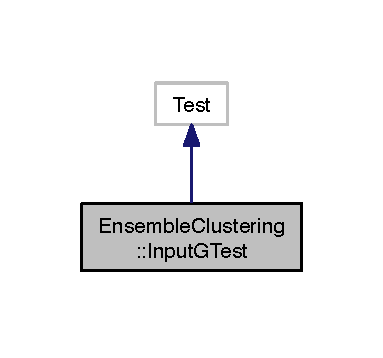
\includegraphics[width=184pt]{class_ensemble_clustering_1_1_input_g_test__inherit__graph}
\end{center}
\end{figure}


Collaboration diagram for Ensemble\-Clustering\-:\-:Input\-G\-Test\-:\nopagebreak
\begin{figure}[H]
\begin{center}
\leavevmode
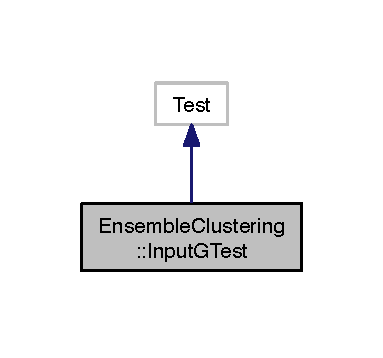
\includegraphics[width=184pt]{class_ensemble_clustering_1_1_input_g_test__coll__graph}
\end{center}
\end{figure}


\subsection{Detailed Description}


Definition at line 18 of file Input\-G\-Test.\-h.



The documentation for this class was generated from the following file\-:\begin{DoxyCompactItemize}
\item 
src/input/test/\hyperlink{_input_g_test_8h}{Input\-G\-Test.\-h}\end{DoxyCompactItemize}

\hypertarget{class_ensemble_clustering_1_1_label_propagation}{\section{Ensemble\-Clustering\-:\-:Label\-Propagation Class Reference}
\label{class_ensemble_clustering_1_1_label_propagation}\index{Ensemble\-Clustering\-::\-Label\-Propagation@{Ensemble\-Clustering\-::\-Label\-Propagation}}
}


As described in Ovelgoenne et al\-: An Ensemble Learning Strategy for \hyperlink{class_ensemble_clustering_1_1_graph}{Graph} \hyperlink{class_ensemble_clustering_1_1_clustering}{Clustering} Raghavan et al.  




{\ttfamily \#include $<$Label\-Propagation.\-h$>$}



Inheritance diagram for Ensemble\-Clustering\-:\-:Label\-Propagation\-:\nopagebreak
\begin{figure}[H]
\begin{center}
\leavevmode
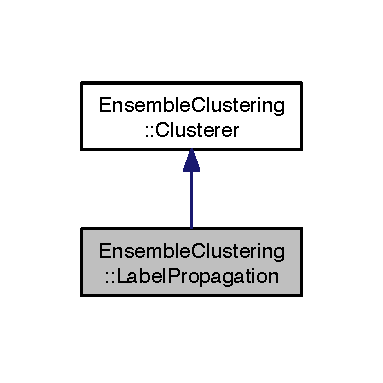
\includegraphics[width=184pt]{class_ensemble_clustering_1_1_label_propagation__inherit__graph}
\end{center}
\end{figure}


Collaboration diagram for Ensemble\-Clustering\-:\-:Label\-Propagation\-:\nopagebreak
\begin{figure}[H]
\begin{center}
\leavevmode
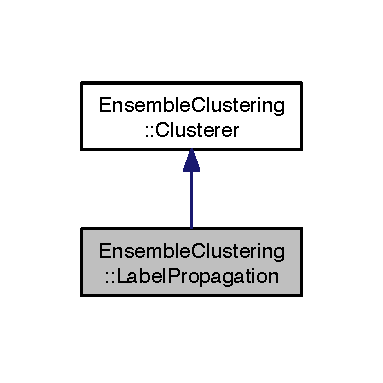
\includegraphics[width=184pt]{class_ensemble_clustering_1_1_label_propagation__coll__graph}
\end{center}
\end{figure}
\subsection*{Public Member Functions}
\begin{DoxyCompactItemize}
\item 
\hyperlink{class_ensemble_clustering_1_1_label_propagation_a72a8f90b8e7632915c729861d320c240}{Label\-Propagation} (\hyperlink{namespace_ensemble_clustering_a2482e94ca22a0c6544a5a9173186fde8}{count} theta=0)
\item 
virtual \hyperlink{class_ensemble_clustering_1_1_label_propagation_a7ac63cb56597fdef47e6c0f4f7b20254}{$\sim$\-Label\-Propagation} ()
\item 
virtual \hyperlink{class_ensemble_clustering_1_1_clustering}{Clustering} \hyperlink{class_ensemble_clustering_1_1_label_propagation_ab6680246bb334e82318703c2ecbbd117}{run} (\hyperlink{class_ensemble_clustering_1_1_graph}{Graph} \&G)
\begin{DoxyCompactList}\small\item\em Run the label propagation clustering algorithm. \end{DoxyCompactList}\item 
virtual std\-::string \hyperlink{class_ensemble_clustering_1_1_label_propagation_a1672735899b9c00e797f0270638fba7f}{to\-String} () const 
\item 
virtual void \hyperlink{class_ensemble_clustering_1_1_label_propagation_adcb4fa1b00aa36461bf3b1c46bc3b892}{set\-Update\-Threshold} (\hyperlink{namespace_ensemble_clustering_a2482e94ca22a0c6544a5a9173186fde8}{count} th)
\begin{DoxyCompactList}\small\item\em The algorithm runs until a number of nodes less than the threshold is updated. \end{DoxyCompactList}\end{DoxyCompactItemize}
\subsection*{Protected Attributes}
\begin{DoxyCompactItemize}
\item 
\hyperlink{namespace_ensemble_clustering_a2482e94ca22a0c6544a5a9173186fde8}{count} \hyperlink{class_ensemble_clustering_1_1_label_propagation_a02e1930c35c9b2fe9121415cb6be7b65}{update\-Threshold} = 0
\end{DoxyCompactItemize}


\subsection{Detailed Description}
As described in Ovelgoenne et al\-: An Ensemble Learning Strategy for \hyperlink{class_ensemble_clustering_1_1_graph}{Graph} \hyperlink{class_ensemble_clustering_1_1_clustering}{Clustering} Raghavan et al. 

proposed a label propagation algorithm for graph clustering. This algorithm initializes every vertex of a graph with a unique label. Then, in iterative sweeps over the set of vertices the vertex labels are updated. A vertex gets the label that the maximum number of its neighbors have. The procedure is stopped when every vertex has the label that at least half of its neighbors have. 

Definition at line 43 of file Label\-Propagation.\-h.



\subsection{Constructor \& Destructor Documentation}
\hypertarget{class_ensemble_clustering_1_1_label_propagation_a72a8f90b8e7632915c729861d320c240}{\index{Ensemble\-Clustering\-::\-Label\-Propagation@{Ensemble\-Clustering\-::\-Label\-Propagation}!Label\-Propagation@{Label\-Propagation}}
\index{Label\-Propagation@{Label\-Propagation}!EnsembleClustering::LabelPropagation@{Ensemble\-Clustering\-::\-Label\-Propagation}}
\subsubsection[{Label\-Propagation}]{\setlength{\rightskip}{0pt plus 5cm}Ensemble\-Clustering\-::\-Label\-Propagation\-::\-Label\-Propagation (
\begin{DoxyParamCaption}
\item[{{\bf count}}]{theta = {\ttfamily 0}}
\end{DoxyParamCaption}
)}}\label{class_ensemble_clustering_1_1_label_propagation_a72a8f90b8e7632915c729861d320c240}


Definition at line 12 of file Label\-Propagation.\-cpp.

\hypertarget{class_ensemble_clustering_1_1_label_propagation_a7ac63cb56597fdef47e6c0f4f7b20254}{\index{Ensemble\-Clustering\-::\-Label\-Propagation@{Ensemble\-Clustering\-::\-Label\-Propagation}!$\sim$\-Label\-Propagation@{$\sim$\-Label\-Propagation}}
\index{$\sim$\-Label\-Propagation@{$\sim$\-Label\-Propagation}!EnsembleClustering::LabelPropagation@{Ensemble\-Clustering\-::\-Label\-Propagation}}
\subsubsection[{$\sim$\-Label\-Propagation}]{\setlength{\rightskip}{0pt plus 5cm}Ensemble\-Clustering\-::\-Label\-Propagation\-::$\sim$\-Label\-Propagation (
\begin{DoxyParamCaption}
{}
\end{DoxyParamCaption}
)\hspace{0.3cm}{\ttfamily [virtual]}}}\label{class_ensemble_clustering_1_1_label_propagation_a7ac63cb56597fdef47e6c0f4f7b20254}


Definition at line 17 of file Label\-Propagation.\-cpp.



\subsection{Member Function Documentation}
\hypertarget{class_ensemble_clustering_1_1_label_propagation_ab6680246bb334e82318703c2ecbbd117}{\index{Ensemble\-Clustering\-::\-Label\-Propagation@{Ensemble\-Clustering\-::\-Label\-Propagation}!run@{run}}
\index{run@{run}!EnsembleClustering::LabelPropagation@{Ensemble\-Clustering\-::\-Label\-Propagation}}
\subsubsection[{run}]{\setlength{\rightskip}{0pt plus 5cm}{\bf Clustering} Ensemble\-Clustering\-::\-Label\-Propagation\-::run (
\begin{DoxyParamCaption}
\item[{{\bf Graph} \&}]{G}
\end{DoxyParamCaption}
)\hspace{0.3cm}{\ttfamily [virtual]}}}\label{class_ensemble_clustering_1_1_label_propagation_ab6680246bb334e82318703c2ecbbd117}


Run the label propagation clustering algorithm. 


\begin{DoxyParams}[1]{Parameters}
\mbox{\tt in}  & {\em G} & input graph \\
\hline
\end{DoxyParams}
\begin{DoxyReturn}{Returns}
clustering 
\end{DoxyReturn}
== Dealing with isolated nodes ==

The pseudocode published does not deal with isolated nodes (and therefore does not terminate if they are present). Isolated nodes stay singletons. They can be ignored in the while loop, but the loop condition must compare to the number of non-\/isolated nodes instead of n.

== Termination criterion ==

The published termination criterion is\-: All nodes have got the label of the majority of their neighbors. In general this does not work. It was changed to\-: No label was changed in last iteration.

Implements \hyperlink{class_ensemble_clustering_1_1_clusterer_a9fab8db7082b6399e1d29509512cad91}{Ensemble\-Clustering\-::\-Clusterer}.



Definition at line 22 of file Label\-Propagation.\-cpp.



Here is the call graph for this function\-:
\nopagebreak
\begin{figure}[H]
\begin{center}
\leavevmode
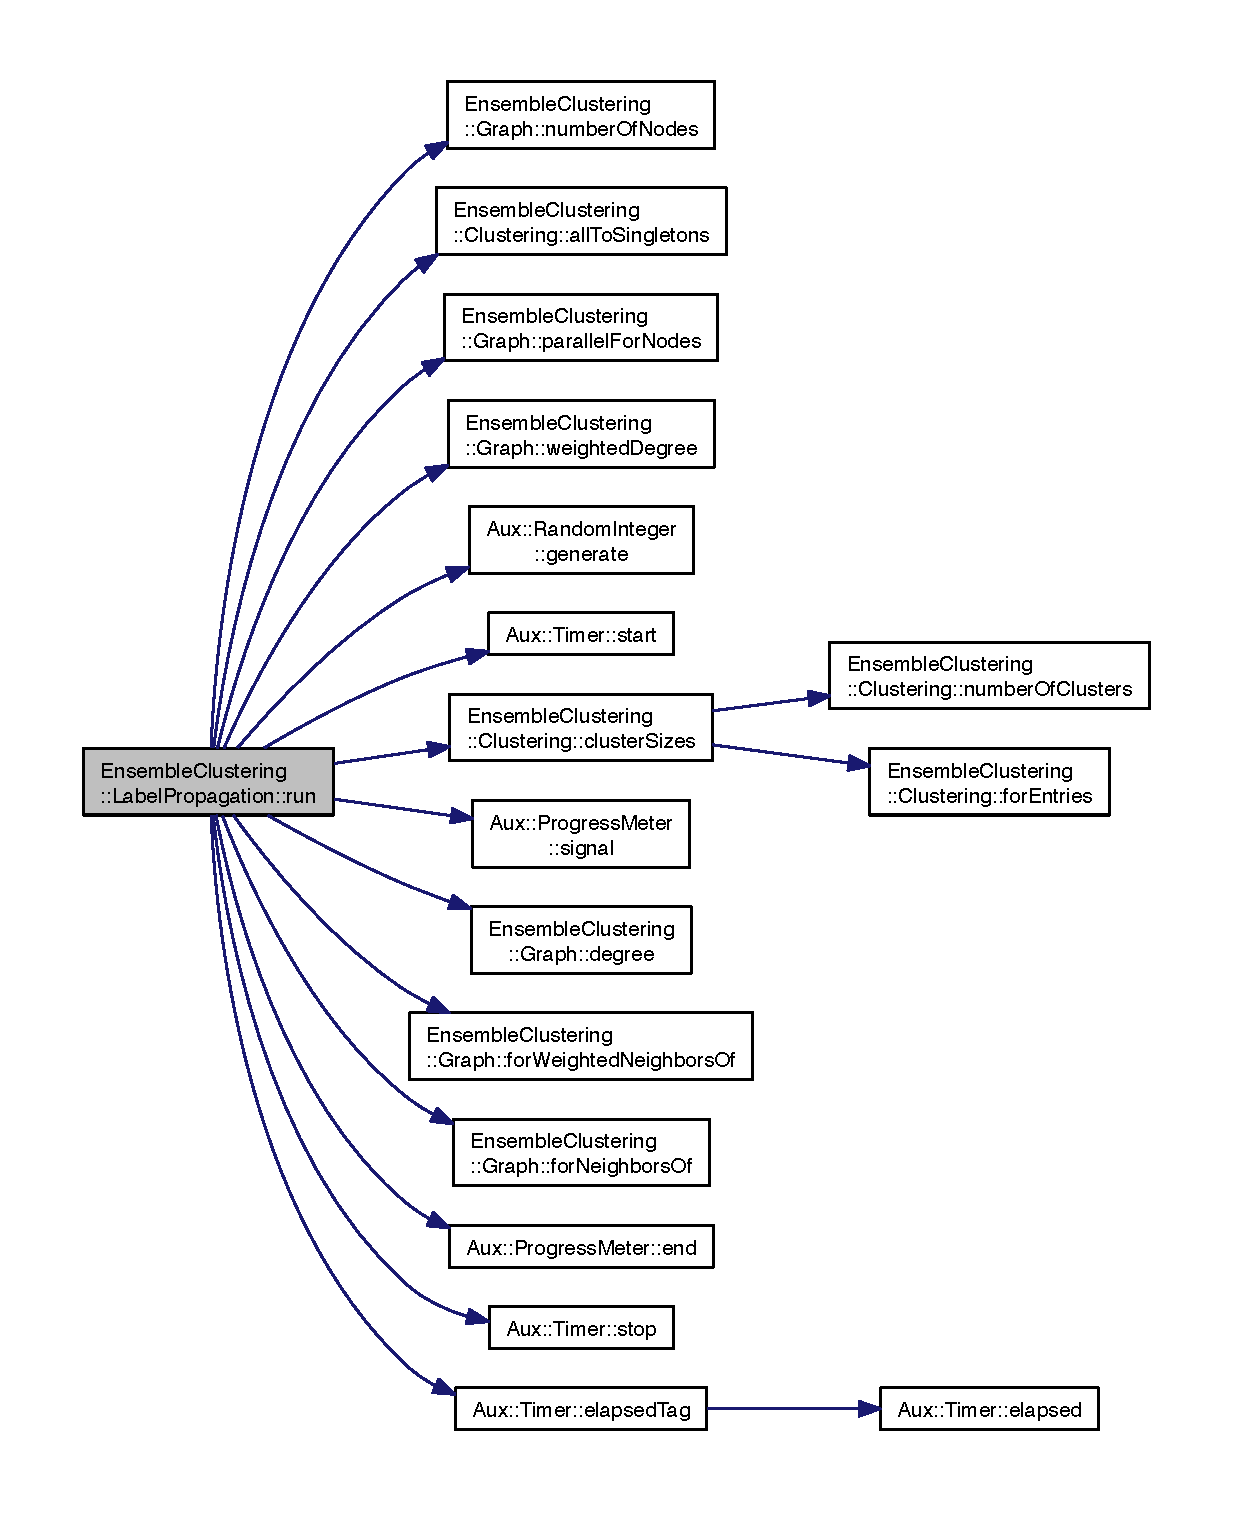
\includegraphics[width=350pt]{class_ensemble_clustering_1_1_label_propagation_ab6680246bb334e82318703c2ecbbd117_cgraph}
\end{center}
\end{figure}


\hypertarget{class_ensemble_clustering_1_1_label_propagation_adcb4fa1b00aa36461bf3b1c46bc3b892}{\index{Ensemble\-Clustering\-::\-Label\-Propagation@{Ensemble\-Clustering\-::\-Label\-Propagation}!set\-Update\-Threshold@{set\-Update\-Threshold}}
\index{set\-Update\-Threshold@{set\-Update\-Threshold}!EnsembleClustering::LabelPropagation@{Ensemble\-Clustering\-::\-Label\-Propagation}}
\subsubsection[{set\-Update\-Threshold}]{\setlength{\rightskip}{0pt plus 5cm}void Ensemble\-Clustering\-::\-Label\-Propagation\-::set\-Update\-Threshold (
\begin{DoxyParamCaption}
\item[{{\bf count}}]{th}
\end{DoxyParamCaption}
)\hspace{0.3cm}{\ttfamily [virtual]}}}\label{class_ensemble_clustering_1_1_label_propagation_adcb4fa1b00aa36461bf3b1c46bc3b892}


The algorithm runs until a number of nodes less than the threshold is updated. 



Definition at line 215 of file Label\-Propagation.\-cpp.

\hypertarget{class_ensemble_clustering_1_1_label_propagation_a1672735899b9c00e797f0270638fba7f}{\index{Ensemble\-Clustering\-::\-Label\-Propagation@{Ensemble\-Clustering\-::\-Label\-Propagation}!to\-String@{to\-String}}
\index{to\-String@{to\-String}!EnsembleClustering::LabelPropagation@{Ensemble\-Clustering\-::\-Label\-Propagation}}
\subsubsection[{to\-String}]{\setlength{\rightskip}{0pt plus 5cm}std\-::string Ensemble\-Clustering\-::\-Label\-Propagation\-::to\-String (
\begin{DoxyParamCaption}
{}
\end{DoxyParamCaption}
) const\hspace{0.3cm}{\ttfamily [virtual]}}}\label{class_ensemble_clustering_1_1_label_propagation_a1672735899b9c00e797f0270638fba7f}
\begin{DoxyReturn}{Returns}
string representation of algorithm and parameters. 
\end{DoxyReturn}


Reimplemented from \hyperlink{class_ensemble_clustering_1_1_clusterer_aba1a37081af12061ef675139668c5ee6}{Ensemble\-Clustering\-::\-Clusterer}.



Definition at line 205 of file Label\-Propagation.\-cpp.



\subsection{Member Data Documentation}
\hypertarget{class_ensemble_clustering_1_1_label_propagation_a02e1930c35c9b2fe9121415cb6be7b65}{\index{Ensemble\-Clustering\-::\-Label\-Propagation@{Ensemble\-Clustering\-::\-Label\-Propagation}!update\-Threshold@{update\-Threshold}}
\index{update\-Threshold@{update\-Threshold}!EnsembleClustering::LabelPropagation@{Ensemble\-Clustering\-::\-Label\-Propagation}}
\subsubsection[{update\-Threshold}]{\setlength{\rightskip}{0pt plus 5cm}{\bf count} Ensemble\-Clustering\-::\-Label\-Propagation\-::update\-Threshold = 0\hspace{0.3cm}{\ttfamily [protected]}}}\label{class_ensemble_clustering_1_1_label_propagation_a02e1930c35c9b2fe9121415cb6be7b65}


Definition at line 47 of file Label\-Propagation.\-h.



The documentation for this class was generated from the following files\-:\begin{DoxyCompactItemize}
\item 
src/community/\hyperlink{_label_propagation_8h}{Label\-Propagation.\-h}\item 
src/community/\hyperlink{_label_propagation_8cpp}{Label\-Propagation.\-cpp}\end{DoxyCompactItemize}

\hypertarget{class_ensemble_clustering_1_1_matcher}{\section{Ensemble\-Clustering\-:\-:Matcher Class Reference}
\label{class_ensemble_clustering_1_1_matcher}\index{Ensemble\-Clustering\-::\-Matcher@{Ensemble\-Clustering\-::\-Matcher}}
}


{\ttfamily \#include $<$Matcher.\-h$>$}



Inheritance diagram for Ensemble\-Clustering\-:\-:Matcher\-:
\nopagebreak
\begin{figure}[H]
\begin{center}
\leavevmode
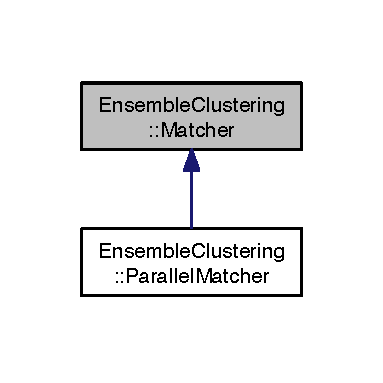
\includegraphics[width=184pt]{class_ensemble_clustering_1_1_matcher__inherit__graph}
\end{center}
\end{figure}
\subsection*{Public Member Functions}
\begin{DoxyCompactItemize}
\item 
\hyperlink{class_ensemble_clustering_1_1_matcher_a0ce4d861d6801323f7fecd299694adae}{Matcher} ()
\item 
virtual \hyperlink{class_ensemble_clustering_1_1_matcher_aeed88dc2dc179e94c36ff3f6472db766}{$\sim$\-Matcher} ()
\item 
virtual \hyperlink{class_ensemble_clustering_1_1_matching}{Matching} \hyperlink{class_ensemble_clustering_1_1_matcher_ab0b3532440faa6678f16ee11a6215b75}{run} (\hyperlink{class_ensemble_clustering_1_1_graph}{Graph} \&G)=0
\end{DoxyCompactItemize}


\subsection{Detailed Description}


Definition at line 16 of file Matcher.\-h.



\subsection{Constructor \& Destructor Documentation}
\hypertarget{class_ensemble_clustering_1_1_matcher_a0ce4d861d6801323f7fecd299694adae}{\index{Ensemble\-Clustering\-::\-Matcher@{Ensemble\-Clustering\-::\-Matcher}!Matcher@{Matcher}}
\index{Matcher@{Matcher}!EnsembleClustering::Matcher@{Ensemble\-Clustering\-::\-Matcher}}
\subsubsection[{Matcher}]{\setlength{\rightskip}{0pt plus 5cm}Ensemble\-Clustering\-::\-Matcher\-::\-Matcher (
\begin{DoxyParamCaption}
{}
\end{DoxyParamCaption}
)}}\label{class_ensemble_clustering_1_1_matcher_a0ce4d861d6801323f7fecd299694adae}


Definition at line 12 of file Matcher.\-cpp.

\hypertarget{class_ensemble_clustering_1_1_matcher_aeed88dc2dc179e94c36ff3f6472db766}{\index{Ensemble\-Clustering\-::\-Matcher@{Ensemble\-Clustering\-::\-Matcher}!$\sim$\-Matcher@{$\sim$\-Matcher}}
\index{$\sim$\-Matcher@{$\sim$\-Matcher}!EnsembleClustering::Matcher@{Ensemble\-Clustering\-::\-Matcher}}
\subsubsection[{$\sim$\-Matcher}]{\setlength{\rightskip}{0pt plus 5cm}Ensemble\-Clustering\-::\-Matcher\-::$\sim$\-Matcher (
\begin{DoxyParamCaption}
{}
\end{DoxyParamCaption}
)\hspace{0.3cm}{\ttfamily [virtual]}}}\label{class_ensemble_clustering_1_1_matcher_aeed88dc2dc179e94c36ff3f6472db766}


Definition at line 17 of file Matcher.\-cpp.



\subsection{Member Function Documentation}
\hypertarget{class_ensemble_clustering_1_1_matcher_ab0b3532440faa6678f16ee11a6215b75}{\index{Ensemble\-Clustering\-::\-Matcher@{Ensemble\-Clustering\-::\-Matcher}!run@{run}}
\index{run@{run}!EnsembleClustering::Matcher@{Ensemble\-Clustering\-::\-Matcher}}
\subsubsection[{run}]{\setlength{\rightskip}{0pt plus 5cm}virtual {\bf Matching} Ensemble\-Clustering\-::\-Matcher\-::run (
\begin{DoxyParamCaption}
\item[{{\bf Graph} \&}]{G}
\end{DoxyParamCaption}
)\hspace{0.3cm}{\ttfamily [pure virtual]}}}\label{class_ensemble_clustering_1_1_matcher_ab0b3532440faa6678f16ee11a6215b75}


Implemented in \hyperlink{class_ensemble_clustering_1_1_parallel_matcher_a59d01ba8833164d22ddf54f5d163d7cb}{Ensemble\-Clustering\-::\-Parallel\-Matcher}.



The documentation for this class was generated from the following files\-:\begin{DoxyCompactItemize}
\item 
src/matching/\hyperlink{_matcher_8h}{Matcher.\-h}\item 
src/matching/\hyperlink{_matcher_8cpp}{Matcher.\-cpp}\end{DoxyCompactItemize}

\hypertarget{class_ensemble_clustering_1_1_matching}{\section{Ensemble\-Clustering\-:\-:Matching Class Reference}
\label{class_ensemble_clustering_1_1_matching}\index{Ensemble\-Clustering\-::\-Matching@{Ensemble\-Clustering\-::\-Matching}}
}


{\ttfamily \#include $<$Matching.\-h$>$}



Inheritance diagram for Ensemble\-Clustering\-:\-:Matching\-:
\nopagebreak
\begin{figure}[H]
\begin{center}
\leavevmode
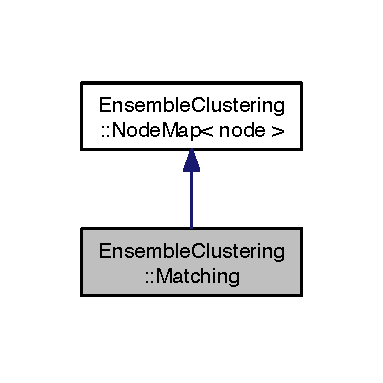
\includegraphics[width=212pt]{class_ensemble_clustering_1_1_matching__inherit__graph}
\end{center}
\end{figure}


Collaboration diagram for Ensemble\-Clustering\-:\-:Matching\-:
\nopagebreak
\begin{figure}[H]
\begin{center}
\leavevmode
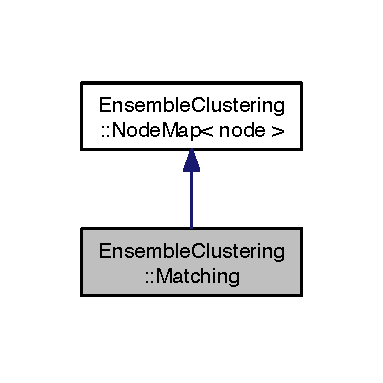
\includegraphics[width=212pt]{class_ensemble_clustering_1_1_matching__coll__graph}
\end{center}
\end{figure}
\subsection*{Public Member Functions}
\begin{DoxyCompactItemize}
\item 
\hyperlink{class_ensemble_clustering_1_1_matching_a5e1de8d09e758fae48909c25484b42b7}{Matching} (int64\-\_\-t \hyperlink{class_ensemble_clustering_1_1_index_map_a3151d302c54e6ad0175bd87aef62d4ca}{n})
\begin{DoxyCompactList}\small\item\em Construct new matching. \end{DoxyCompactList}\item 
virtual \hyperlink{class_ensemble_clustering_1_1_matching_abcc136cf0a7e0b0f2364f2d1b3eb1f2c}{$\sim$\-Matching} ()
\begin{DoxyCompactList}\small\item\em Destructor. \end{DoxyCompactList}\item 
void \hyperlink{class_ensemble_clustering_1_1_matching_a41f6ed1f3b1660fb682c32cf2ade11de}{match} (const \hyperlink{namespace_ensemble_clustering_ae829290aeccd1a420b17a37fd901f114}{node} \&u, const \hyperlink{namespace_ensemble_clustering_ae829290aeccd1a420b17a37fd901f114}{node} \&v)
\begin{DoxyCompactList}\small\item\em Set two nodes as eachothers matching partners. \end{DoxyCompactList}\item 
void \hyperlink{class_ensemble_clustering_1_1_matching_a214fd9e80cb5842f87e2ec909655b5e2}{unmatch} (const \hyperlink{namespace_ensemble_clustering_ae829290aeccd1a420b17a37fd901f114}{node} \&u, const \hyperlink{namespace_ensemble_clustering_ae829290aeccd1a420b17a37fd901f114}{node} \&v)
\begin{DoxyCompactList}\small\item\em Reset the two nodes to unmatched. \end{DoxyCompactList}\item 
bool \hyperlink{class_ensemble_clustering_1_1_matching_a6591583cd8dcd8ddc702cdbddcc42bd0}{is\-Matched} (const \hyperlink{namespace_ensemble_clustering_ae829290aeccd1a420b17a37fd901f114}{node} \&u) const 
\begin{DoxyCompactList}\small\item\em Check if node is matched. \end{DoxyCompactList}\item 
bool \hyperlink{class_ensemble_clustering_1_1_matching_ad2637dece8a3a56d9f62f3c9df4713db}{are\-Matched} (const \hyperlink{namespace_ensemble_clustering_ae829290aeccd1a420b17a37fd901f114}{node} \&u, const \hyperlink{namespace_ensemble_clustering_ae829290aeccd1a420b17a37fd901f114}{node} \&v) const 
\begin{DoxyCompactList}\small\item\em Check if the two nodes are matched. \end{DoxyCompactList}\item 
bool \hyperlink{class_ensemble_clustering_1_1_matching_a29b8fa3ba916f0b3d73b184c883c36b6}{is\-Proper} (\hyperlink{class_ensemble_clustering_1_1_graph}{Graph} \&G) const 
\begin{DoxyCompactList}\small\item\em Check whether this is a proper matching in the graph, i.\-e. \end{DoxyCompactList}\item 
\hyperlink{class_ensemble_clustering_1_1_matching}{Matching} \& \hyperlink{class_ensemble_clustering_1_1_matching_aa1d0732ec84c2012fd3e642595f23556}{operator=} (const \hyperlink{class_ensemble_clustering_1_1_matching}{Matching} \&from)
\begin{DoxyCompactList}\small\item\em copy semantics \end{DoxyCompactList}\item 
void \hyperlink{class_ensemble_clustering_1_1_matching_a6753fd67c53b6e0d94f2d6e0d6de640e}{clone} (const \hyperlink{class_ensemble_clustering_1_1_matching}{Matching} \&from)
\begin{DoxyCompactList}\small\item\em Properly copy this object. \end{DoxyCompactList}\item 
void \hyperlink{class_ensemble_clustering_1_1_matching_ae7e8c62662439dc7adae829506d2dd32}{dispose} ()
\begin{DoxyCompactList}\small\item\em Properly destruct this object. \end{DoxyCompactList}\item 
\hyperlink{namespace_ensemble_clustering_a2482e94ca22a0c6544a5a9173186fde8}{count} \hyperlink{class_ensemble_clustering_1_1_matching_a0e9020a85e9f6e8d0bf0ec236394b2e8}{matching\-Size} () const 
\item 
\hyperlink{namespace_ensemble_clustering_a1ba11e6d628873b803a26fe054f45e28}{index} \hyperlink{class_ensemble_clustering_1_1_matching_adc5f7971cb778e55e58b140e1371b89d}{mate} (\hyperlink{namespace_ensemble_clustering_ae829290aeccd1a420b17a37fd901f114}{node} v) const 
\end{DoxyCompactItemize}
\subsection*{Additional Inherited Members}


\subsection{Detailed Description}


Definition at line 17 of file Matching.\-h.



\subsection{Constructor \& Destructor Documentation}
\hypertarget{class_ensemble_clustering_1_1_matching_a5e1de8d09e758fae48909c25484b42b7}{\index{Ensemble\-Clustering\-::\-Matching@{Ensemble\-Clustering\-::\-Matching}!Matching@{Matching}}
\index{Matching@{Matching}!EnsembleClustering::Matching@{Ensemble\-Clustering\-::\-Matching}}
\subsubsection[{Matching}]{\setlength{\rightskip}{0pt plus 5cm}Ensemble\-Clustering\-::\-Matching\-::\-Matching (
\begin{DoxyParamCaption}
\item[{int64\-\_\-t}]{n}
\end{DoxyParamCaption}
)}}\label{class_ensemble_clustering_1_1_matching_a5e1de8d09e758fae48909c25484b42b7}


Construct new matching. 


\begin{DoxyParams}[1]{Parameters}
\mbox{\tt in}  & {\em n} & maximum number of nodes \\
\hline
\end{DoxyParams}


Definition at line 12 of file Matching.\-cpp.

\hypertarget{class_ensemble_clustering_1_1_matching_abcc136cf0a7e0b0f2364f2d1b3eb1f2c}{\index{Ensemble\-Clustering\-::\-Matching@{Ensemble\-Clustering\-::\-Matching}!$\sim$\-Matching@{$\sim$\-Matching}}
\index{$\sim$\-Matching@{$\sim$\-Matching}!EnsembleClustering::Matching@{Ensemble\-Clustering\-::\-Matching}}
\subsubsection[{$\sim$\-Matching}]{\setlength{\rightskip}{0pt plus 5cm}Ensemble\-Clustering\-::\-Matching\-::$\sim$\-Matching (
\begin{DoxyParamCaption}
{}
\end{DoxyParamCaption}
)\hspace{0.3cm}{\ttfamily [virtual]}}}\label{class_ensemble_clustering_1_1_matching_abcc136cf0a7e0b0f2364f2d1b3eb1f2c}


Destructor. 



Definition at line 20 of file Matching.\-cpp.



\subsection{Member Function Documentation}
\hypertarget{class_ensemble_clustering_1_1_matching_ad2637dece8a3a56d9f62f3c9df4713db}{\index{Ensemble\-Clustering\-::\-Matching@{Ensemble\-Clustering\-::\-Matching}!are\-Matched@{are\-Matched}}
\index{are\-Matched@{are\-Matched}!EnsembleClustering::Matching@{Ensemble\-Clustering\-::\-Matching}}
\subsubsection[{are\-Matched}]{\setlength{\rightskip}{0pt plus 5cm}bool Ensemble\-Clustering\-::\-Matching\-::are\-Matched (
\begin{DoxyParamCaption}
\item[{const {\bf node} \&}]{u, }
\item[{const {\bf node} \&}]{v}
\end{DoxyParamCaption}
) const}}\label{class_ensemble_clustering_1_1_matching_ad2637dece8a3a56d9f62f3c9df4713db}


Check if the two nodes are matched. 



Definition at line 70 of file Matching.\-cpp.

\hypertarget{class_ensemble_clustering_1_1_matching_a6753fd67c53b6e0d94f2d6e0d6de640e}{\index{Ensemble\-Clustering\-::\-Matching@{Ensemble\-Clustering\-::\-Matching}!clone@{clone}}
\index{clone@{clone}!EnsembleClustering::Matching@{Ensemble\-Clustering\-::\-Matching}}
\subsubsection[{clone}]{\setlength{\rightskip}{0pt plus 5cm}void Ensemble\-Clustering\-::\-Matching\-::clone (
\begin{DoxyParamCaption}
\item[{const {\bf Matching} \&}]{from}
\end{DoxyParamCaption}
)}}\label{class_ensemble_clustering_1_1_matching_a6753fd67c53b6e0d94f2d6e0d6de640e}


Properly copy this object. 

\hypertarget{class_ensemble_clustering_1_1_matching_ae7e8c62662439dc7adae829506d2dd32}{\index{Ensemble\-Clustering\-::\-Matching@{Ensemble\-Clustering\-::\-Matching}!dispose@{dispose}}
\index{dispose@{dispose}!EnsembleClustering::Matching@{Ensemble\-Clustering\-::\-Matching}}
\subsubsection[{dispose}]{\setlength{\rightskip}{0pt plus 5cm}void Ensemble\-Clustering\-::\-Matching\-::dispose (
\begin{DoxyParamCaption}
{}
\end{DoxyParamCaption}
)}}\label{class_ensemble_clustering_1_1_matching_ae7e8c62662439dc7adae829506d2dd32}


Properly destruct this object. 

\hypertarget{class_ensemble_clustering_1_1_matching_a6591583cd8dcd8ddc702cdbddcc42bd0}{\index{Ensemble\-Clustering\-::\-Matching@{Ensemble\-Clustering\-::\-Matching}!is\-Matched@{is\-Matched}}
\index{is\-Matched@{is\-Matched}!EnsembleClustering::Matching@{Ensemble\-Clustering\-::\-Matching}}
\subsubsection[{is\-Matched}]{\setlength{\rightskip}{0pt plus 5cm}bool Ensemble\-Clustering\-::\-Matching\-::is\-Matched (
\begin{DoxyParamCaption}
\item[{const {\bf node} \&}]{u}
\end{DoxyParamCaption}
) const}}\label{class_ensemble_clustering_1_1_matching_a6591583cd8dcd8ddc702cdbddcc42bd0}


Check if node is matched. 


\begin{DoxyParams}[1]{Parameters}
\mbox{\tt in}  & {\em u} & a node \\
\hline
\mbox{\tt out}  & {\em true} & if u is matched \\
\hline
\end{DoxyParams}


Definition at line 23 of file Matching.\-cpp.

\hypertarget{class_ensemble_clustering_1_1_matching_a29b8fa3ba916f0b3d73b184c883c36b6}{\index{Ensemble\-Clustering\-::\-Matching@{Ensemble\-Clustering\-::\-Matching}!is\-Proper@{is\-Proper}}
\index{is\-Proper@{is\-Proper}!EnsembleClustering::Matching@{Ensemble\-Clustering\-::\-Matching}}
\subsubsection[{is\-Proper}]{\setlength{\rightskip}{0pt plus 5cm}bool Ensemble\-Clustering\-::\-Matching\-::is\-Proper (
\begin{DoxyParamCaption}
\item[{{\bf Graph} \&}]{G}
\end{DoxyParamCaption}
) const}}\label{class_ensemble_clustering_1_1_matching_a29b8fa3ba916f0b3d73b184c883c36b6}


Check whether this is a proper matching in the graph, i.\-e. 

no two edges are adjacent.

\mbox{[}in\mbox{]} G a graph 
\begin{DoxyParams}[1]{Parameters}
\mbox{\tt out}  & {\em true} & if this is a proper matching \\
\hline
\end{DoxyParams}
The content of this data structure represents a matching iff (for all v in V\-: M\mbox{[}v\mbox{]} = v or M\mbox{[}M\mbox{[}v\mbox{]}\mbox{]} = v) and (for all (u,v) in M)\-: (u,v) in E

Definition at line 27 of file Matching.\-cpp.



Here is the call graph for this function\-:
\nopagebreak
\begin{figure}[H]
\begin{center}
\leavevmode
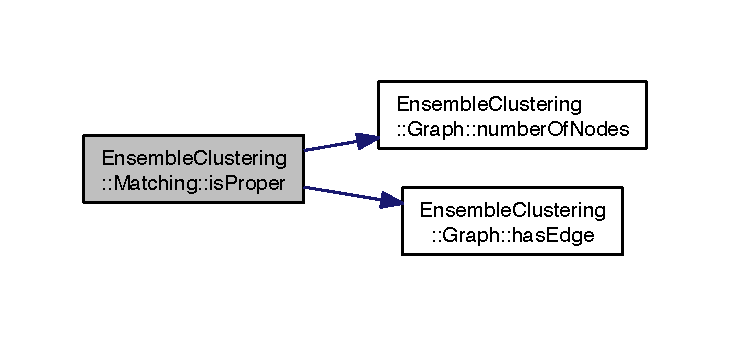
\includegraphics[width=350pt]{class_ensemble_clustering_1_1_matching_a29b8fa3ba916f0b3d73b184c883c36b6_cgraph}
\end{center}
\end{figure}


\hypertarget{class_ensemble_clustering_1_1_matching_a41f6ed1f3b1660fb682c32cf2ade11de}{\index{Ensemble\-Clustering\-::\-Matching@{Ensemble\-Clustering\-::\-Matching}!match@{match}}
\index{match@{match}!EnsembleClustering::Matching@{Ensemble\-Clustering\-::\-Matching}}
\subsubsection[{match}]{\setlength{\rightskip}{0pt plus 5cm}void Ensemble\-Clustering\-::\-Matching\-::match (
\begin{DoxyParamCaption}
\item[{const {\bf node} \&}]{u, }
\item[{const {\bf node} \&}]{v}
\end{DoxyParamCaption}
)}}\label{class_ensemble_clustering_1_1_matching_a41f6ed1f3b1660fb682c32cf2ade11de}


Set two nodes as eachothers matching partners. 



Definition at line 60 of file Matching.\-cpp.

\hypertarget{class_ensemble_clustering_1_1_matching_a0e9020a85e9f6e8d0bf0ec236394b2e8}{\index{Ensemble\-Clustering\-::\-Matching@{Ensemble\-Clustering\-::\-Matching}!matching\-Size@{matching\-Size}}
\index{matching\-Size@{matching\-Size}!EnsembleClustering::Matching@{Ensemble\-Clustering\-::\-Matching}}
\subsubsection[{matching\-Size}]{\setlength{\rightskip}{0pt plus 5cm}{\bf count} Ensemble\-Clustering\-::\-Matching\-::matching\-Size (
\begin{DoxyParamCaption}
{}
\end{DoxyParamCaption}
) const}}\label{class_ensemble_clustering_1_1_matching_a0e9020a85e9f6e8d0bf0ec236394b2e8}
\begin{DoxyReturn}{Returns}
Number of edges in matching. 
\end{DoxyReturn}


Definition at line 74 of file Matching.\-cpp.



Here is the call graph for this function\-:
\nopagebreak
\begin{figure}[H]
\begin{center}
\leavevmode
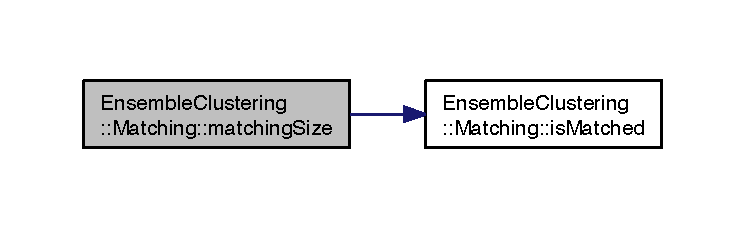
\includegraphics[width=350pt]{class_ensemble_clustering_1_1_matching_a0e9020a85e9f6e8d0bf0ec236394b2e8_cgraph}
\end{center}
\end{figure}


\hypertarget{class_ensemble_clustering_1_1_matching_adc5f7971cb778e55e58b140e1371b89d}{\index{Ensemble\-Clustering\-::\-Matching@{Ensemble\-Clustering\-::\-Matching}!mate@{mate}}
\index{mate@{mate}!EnsembleClustering::Matching@{Ensemble\-Clustering\-::\-Matching}}
\subsubsection[{mate}]{\setlength{\rightskip}{0pt plus 5cm}{\bf index} Ensemble\-Clustering\-::\-Matching\-::mate (
\begin{DoxyParamCaption}
\item[{{\bf node}}]{v}
\end{DoxyParamCaption}
) const}}\label{class_ensemble_clustering_1_1_matching_adc5f7971cb778e55e58b140e1371b89d}
\begin{DoxyReturn}{Returns}
Mate of {\itshape v} if it exists, otherwise none. 
\end{DoxyReturn}


Definition at line 84 of file Matching.\-cpp.



Here is the call graph for this function\-:
\nopagebreak
\begin{figure}[H]
\begin{center}
\leavevmode
\includegraphics[width=336pt]{class_ensemble_clustering_1_1_matching_adc5f7971cb778e55e58b140e1371b89d_cgraph}
\end{center}
\end{figure}


\hypertarget{class_ensemble_clustering_1_1_matching_aa1d0732ec84c2012fd3e642595f23556}{\index{Ensemble\-Clustering\-::\-Matching@{Ensemble\-Clustering\-::\-Matching}!operator=@{operator=}}
\index{operator=@{operator=}!EnsembleClustering::Matching@{Ensemble\-Clustering\-::\-Matching}}
\subsubsection[{operator=}]{\setlength{\rightskip}{0pt plus 5cm}{\bf Matching}\& Ensemble\-Clustering\-::\-Matching\-::operator= (
\begin{DoxyParamCaption}
\item[{const {\bf Matching} \&}]{from}
\end{DoxyParamCaption}
)}}\label{class_ensemble_clustering_1_1_matching_aa1d0732ec84c2012fd3e642595f23556}


copy semantics 

Assignment operator. \hypertarget{class_ensemble_clustering_1_1_matching_a214fd9e80cb5842f87e2ec909655b5e2}{\index{Ensemble\-Clustering\-::\-Matching@{Ensemble\-Clustering\-::\-Matching}!unmatch@{unmatch}}
\index{unmatch@{unmatch}!EnsembleClustering::Matching@{Ensemble\-Clustering\-::\-Matching}}
\subsubsection[{unmatch}]{\setlength{\rightskip}{0pt plus 5cm}void Ensemble\-Clustering\-::\-Matching\-::unmatch (
\begin{DoxyParamCaption}
\item[{const {\bf node} \&}]{u, }
\item[{const {\bf node} \&}]{v}
\end{DoxyParamCaption}
)}}\label{class_ensemble_clustering_1_1_matching_a214fd9e80cb5842f87e2ec909655b5e2}


Reset the two nodes to unmatched. 



Definition at line 65 of file Matching.\-cpp.



The documentation for this class was generated from the following files\-:\begin{DoxyCompactItemize}
\item 
src/matching/\hyperlink{_matching_8h}{Matching.\-h}\item 
src/matching/\hyperlink{_matching_8cpp}{Matching.\-cpp}\end{DoxyCompactItemize}

\hypertarget{class_ensemble_clustering_1_1_matching_contracter}{\section{Ensemble\-Clustering\-:\-:Matching\-Contracter Class Reference}
\label{class_ensemble_clustering_1_1_matching_contracter}\index{Ensemble\-Clustering\-::\-Matching\-Contracter@{Ensemble\-Clustering\-::\-Matching\-Contracter}}
}


{\ttfamily \#include $<$Matching\-Contracter.\-h$>$}

\subsection*{Public Member Functions}
\begin{DoxyCompactItemize}
\item 
\hyperlink{class_ensemble_clustering_1_1_matching_contracter_adf9bd1fa8b62171910543e82f8237d71}{Matching\-Contracter} ()
\item 
virtual \hyperlink{class_ensemble_clustering_1_1_matching_contracter_ab04bb205ff8cd3a81a0cfa386094fab6}{$\sim$\-Matching\-Contracter} ()
\end{DoxyCompactItemize}


\subsection{Detailed Description}


Definition at line 13 of file Matching\-Contracter.\-h.



\subsection{Constructor \& Destructor Documentation}
\hypertarget{class_ensemble_clustering_1_1_matching_contracter_adf9bd1fa8b62171910543e82f8237d71}{\index{Ensemble\-Clustering\-::\-Matching\-Contracter@{Ensemble\-Clustering\-::\-Matching\-Contracter}!Matching\-Contracter@{Matching\-Contracter}}
\index{Matching\-Contracter@{Matching\-Contracter}!EnsembleClustering::MatchingContracter@{Ensemble\-Clustering\-::\-Matching\-Contracter}}
\subsubsection[{Matching\-Contracter}]{\setlength{\rightskip}{0pt plus 5cm}Ensemble\-Clustering\-::\-Matching\-Contracter\-::\-Matching\-Contracter (
\begin{DoxyParamCaption}
{}
\end{DoxyParamCaption}
)}}\label{class_ensemble_clustering_1_1_matching_contracter_adf9bd1fa8b62171910543e82f8237d71}


Definition at line 12 of file Matching\-Contracter.\-cpp.

\hypertarget{class_ensemble_clustering_1_1_matching_contracter_ab04bb205ff8cd3a81a0cfa386094fab6}{\index{Ensemble\-Clustering\-::\-Matching\-Contracter@{Ensemble\-Clustering\-::\-Matching\-Contracter}!$\sim$\-Matching\-Contracter@{$\sim$\-Matching\-Contracter}}
\index{$\sim$\-Matching\-Contracter@{$\sim$\-Matching\-Contracter}!EnsembleClustering::MatchingContracter@{Ensemble\-Clustering\-::\-Matching\-Contracter}}
\subsubsection[{$\sim$\-Matching\-Contracter}]{\setlength{\rightskip}{0pt plus 5cm}Ensemble\-Clustering\-::\-Matching\-Contracter\-::$\sim$\-Matching\-Contracter (
\begin{DoxyParamCaption}
{}
\end{DoxyParamCaption}
)\hspace{0.3cm}{\ttfamily [virtual]}}}\label{class_ensemble_clustering_1_1_matching_contracter_ab04bb205ff8cd3a81a0cfa386094fab6}


Definition at line 17 of file Matching\-Contracter.\-cpp.



The documentation for this class was generated from the following files\-:\begin{DoxyCompactItemize}
\item 
src/coarsening/\hyperlink{_matching_contracter_8h}{Matching\-Contracter.\-h}\item 
src/coarsening/\hyperlink{_matching_contracter_8cpp}{Matching\-Contracter.\-cpp}\end{DoxyCompactItemize}

\hypertarget{class_ensemble_clustering_1_1_m_e_t_i_s_parser}{\section{Ensemble\-Clustering\-:\-:M\-E\-T\-I\-S\-Parser Class Reference}
\label{class_ensemble_clustering_1_1_m_e_t_i_s_parser}\index{Ensemble\-Clustering\-::\-M\-E\-T\-I\-S\-Parser@{Ensemble\-Clustering\-::\-M\-E\-T\-I\-S\-Parser}}
}


{\ttfamily \#include $<$M\-E\-T\-I\-S\-Parser.\-h$>$}

\subsection*{Public Member Functions}
\begin{DoxyCompactItemize}
\item 
\hyperlink{class_ensemble_clustering_1_1_m_e_t_i_s_parser_ae805ea274382960d50a6a4cab78272fd}{M\-E\-T\-I\-S\-Parser} (std\-::string path)
\item 
virtual \hyperlink{class_ensemble_clustering_1_1_m_e_t_i_s_parser_a5937df5903a58e15c0df1445a70fff5c}{$\sim$\-M\-E\-T\-I\-S\-Parser} ()
\item 
std\-::pair$<$ int, int $>$ \hyperlink{class_ensemble_clustering_1_1_m_e_t_i_s_parser_a6c11f188b2ca67435a63fc9c71d261e9}{get\-Header} ()
\begin{DoxyCompactList}\small\item\em Get the M\-E\-T\-I\-S graph file header. \end{DoxyCompactList}\item 
bool \hyperlink{class_ensemble_clustering_1_1_m_e_t_i_s_parser_aa9adb857b8ff519edfe94b7bc59ef12a}{has\-Next} ()
\begin{DoxyCompactList}\small\item\em Test if graph file has a next line. \end{DoxyCompactList}\item 
std\-::vector$<$ \hyperlink{namespace_ensemble_clustering_ae829290aeccd1a420b17a37fd901f114}{node} $>$ \hyperlink{class_ensemble_clustering_1_1_m_e_t_i_s_parser_a473d40949f87385130369a4f5d14b2ae}{get\-Next} ()
\begin{DoxyCompactList}\small\item\em Get adjacencies from the next line in the M\-E\-T\-I\-S graph file. \end{DoxyCompactList}\end{DoxyCompactItemize}
\subsection*{Protected Attributes}
\begin{DoxyCompactItemize}
\item 
std\-::ifstream \hyperlink{class_ensemble_clustering_1_1_m_e_t_i_s_parser_abe77511f89d17b6a043d38790b334151}{graph\-File}
\end{DoxyCompactItemize}


\subsection{Detailed Description}


Definition at line 27 of file M\-E\-T\-I\-S\-Parser.\-h.



\subsection{Constructor \& Destructor Documentation}
\hypertarget{class_ensemble_clustering_1_1_m_e_t_i_s_parser_ae805ea274382960d50a6a4cab78272fd}{\index{Ensemble\-Clustering\-::\-M\-E\-T\-I\-S\-Parser@{Ensemble\-Clustering\-::\-M\-E\-T\-I\-S\-Parser}!M\-E\-T\-I\-S\-Parser@{M\-E\-T\-I\-S\-Parser}}
\index{M\-E\-T\-I\-S\-Parser@{M\-E\-T\-I\-S\-Parser}!EnsembleClustering::METISParser@{Ensemble\-Clustering\-::\-M\-E\-T\-I\-S\-Parser}}
\subsubsection[{M\-E\-T\-I\-S\-Parser}]{\setlength{\rightskip}{0pt plus 5cm}Ensemble\-Clustering\-::\-M\-E\-T\-I\-S\-Parser\-::\-M\-E\-T\-I\-S\-Parser (
\begin{DoxyParamCaption}
\item[{std\-::string}]{path}
\end{DoxyParamCaption}
)}}\label{class_ensemble_clustering_1_1_m_e_t_i_s_parser_ae805ea274382960d50a6a4cab78272fd}


Definition at line 63 of file M\-E\-T\-I\-S\-Parser.\-cpp.

\hypertarget{class_ensemble_clustering_1_1_m_e_t_i_s_parser_a5937df5903a58e15c0df1445a70fff5c}{\index{Ensemble\-Clustering\-::\-M\-E\-T\-I\-S\-Parser@{Ensemble\-Clustering\-::\-M\-E\-T\-I\-S\-Parser}!$\sim$\-M\-E\-T\-I\-S\-Parser@{$\sim$\-M\-E\-T\-I\-S\-Parser}}
\index{$\sim$\-M\-E\-T\-I\-S\-Parser@{$\sim$\-M\-E\-T\-I\-S\-Parser}!EnsembleClustering::METISParser@{Ensemble\-Clustering\-::\-M\-E\-T\-I\-S\-Parser}}
\subsubsection[{$\sim$\-M\-E\-T\-I\-S\-Parser}]{\setlength{\rightskip}{0pt plus 5cm}Ensemble\-Clustering\-::\-M\-E\-T\-I\-S\-Parser\-::$\sim$\-M\-E\-T\-I\-S\-Parser (
\begin{DoxyParamCaption}
{}
\end{DoxyParamCaption}
)\hspace{0.3cm}{\ttfamily [virtual]}}}\label{class_ensemble_clustering_1_1_m_e_t_i_s_parser_a5937df5903a58e15c0df1445a70fff5c}


Definition at line 72 of file M\-E\-T\-I\-S\-Parser.\-cpp.



\subsection{Member Function Documentation}
\hypertarget{class_ensemble_clustering_1_1_m_e_t_i_s_parser_a6c11f188b2ca67435a63fc9c71d261e9}{\index{Ensemble\-Clustering\-::\-M\-E\-T\-I\-S\-Parser@{Ensemble\-Clustering\-::\-M\-E\-T\-I\-S\-Parser}!get\-Header@{get\-Header}}
\index{get\-Header@{get\-Header}!EnsembleClustering::METISParser@{Ensemble\-Clustering\-::\-M\-E\-T\-I\-S\-Parser}}
\subsubsection[{get\-Header}]{\setlength{\rightskip}{0pt plus 5cm}std\-::pair$<$ int, int $>$ Ensemble\-Clustering\-::\-M\-E\-T\-I\-S\-Parser\-::get\-Header (
\begin{DoxyParamCaption}
{}
\end{DoxyParamCaption}
)}}\label{class_ensemble_clustering_1_1_m_e_t_i_s_parser_a6c11f188b2ca67435a63fc9c71d261e9}


Get the M\-E\-T\-I\-S graph file header. 



Definition at line 79 of file M\-E\-T\-I\-S\-Parser.\-cpp.

\hypertarget{class_ensemble_clustering_1_1_m_e_t_i_s_parser_a473d40949f87385130369a4f5d14b2ae}{\index{Ensemble\-Clustering\-::\-M\-E\-T\-I\-S\-Parser@{Ensemble\-Clustering\-::\-M\-E\-T\-I\-S\-Parser}!get\-Next@{get\-Next}}
\index{get\-Next@{get\-Next}!EnsembleClustering::METISParser@{Ensemble\-Clustering\-::\-M\-E\-T\-I\-S\-Parser}}
\subsubsection[{get\-Next}]{\setlength{\rightskip}{0pt plus 5cm}std\-::vector$<$ {\bf node} $>$ Ensemble\-Clustering\-::\-M\-E\-T\-I\-S\-Parser\-::get\-Next (
\begin{DoxyParamCaption}
{}
\end{DoxyParamCaption}
)}}\label{class_ensemble_clustering_1_1_m_e_t_i_s_parser_a473d40949f87385130369a4f5d14b2ae}


Get adjacencies from the next line in the M\-E\-T\-I\-S graph file. 



Definition at line 113 of file M\-E\-T\-I\-S\-Parser.\-cpp.

\hypertarget{class_ensemble_clustering_1_1_m_e_t_i_s_parser_aa9adb857b8ff519edfe94b7bc59ef12a}{\index{Ensemble\-Clustering\-::\-M\-E\-T\-I\-S\-Parser@{Ensemble\-Clustering\-::\-M\-E\-T\-I\-S\-Parser}!has\-Next@{has\-Next}}
\index{has\-Next@{has\-Next}!EnsembleClustering::METISParser@{Ensemble\-Clustering\-::\-M\-E\-T\-I\-S\-Parser}}
\subsubsection[{has\-Next}]{\setlength{\rightskip}{0pt plus 5cm}bool Ensemble\-Clustering\-::\-M\-E\-T\-I\-S\-Parser\-::has\-Next (
\begin{DoxyParamCaption}
{}
\end{DoxyParamCaption}
)}}\label{class_ensemble_clustering_1_1_m_e_t_i_s_parser_aa9adb857b8ff519edfe94b7bc59ef12a}


Test if graph file has a next line. 



Definition at line 107 of file M\-E\-T\-I\-S\-Parser.\-cpp.



\subsection{Member Data Documentation}
\hypertarget{class_ensemble_clustering_1_1_m_e_t_i_s_parser_abe77511f89d17b6a043d38790b334151}{\index{Ensemble\-Clustering\-::\-M\-E\-T\-I\-S\-Parser@{Ensemble\-Clustering\-::\-M\-E\-T\-I\-S\-Parser}!graph\-File@{graph\-File}}
\index{graph\-File@{graph\-File}!EnsembleClustering::METISParser@{Ensemble\-Clustering\-::\-M\-E\-T\-I\-S\-Parser}}
\subsubsection[{graph\-File}]{\setlength{\rightskip}{0pt plus 5cm}std\-::ifstream Ensemble\-Clustering\-::\-M\-E\-T\-I\-S\-Parser\-::graph\-File\hspace{0.3cm}{\ttfamily [protected]}}}\label{class_ensemble_clustering_1_1_m_e_t_i_s_parser_abe77511f89d17b6a043d38790b334151}


Definition at line 32 of file M\-E\-T\-I\-S\-Parser.\-h.



The documentation for this class was generated from the following files\-:\begin{DoxyCompactItemize}
\item 
src/io/\hyperlink{_m_e_t_i_s_parser_8h}{M\-E\-T\-I\-S\-Parser.\-h}\item 
src/io/\hyperlink{_m_e_t_i_s_parser_8cpp}{M\-E\-T\-I\-S\-Parser.\-cpp}\end{DoxyCompactItemize}

\hypertarget{class_ensemble_clustering_1_1_m_e_t_i_sto_s_t_i_n_g_e_r}{\section{Ensemble\-Clustering\-:\-:M\-E\-T\-I\-Sto\-S\-T\-I\-N\-G\-E\-R Class Reference}
\label{class_ensemble_clustering_1_1_m_e_t_i_sto_s_t_i_n_g_e_r}\index{Ensemble\-Clustering\-::\-M\-E\-T\-I\-Sto\-S\-T\-I\-N\-G\-E\-R@{Ensemble\-Clustering\-::\-M\-E\-T\-I\-Sto\-S\-T\-I\-N\-G\-E\-R}}
}


This class provides a user interface for reading a M\-E\-T\-I\-S graph file and returning a S\-T\-I\-N\-G\-E\-R-\/based graph object.  




{\ttfamily \#include $<$M\-E\-T\-I\-Sto\-S\-T\-I\-N\-G\-E\-R.\-h$>$}

\subsection*{Public Member Functions}
\begin{DoxyCompactItemize}
\item 
\hyperlink{class_ensemble_clustering_1_1_m_e_t_i_sto_s_t_i_n_g_e_r_af4f8ac58e71d795429ed9f2eeded23f9}{M\-E\-T\-I\-Sto\-S\-T\-I\-N\-G\-E\-R} ()
\item 
virtual \hyperlink{class_ensemble_clustering_1_1_m_e_t_i_sto_s_t_i_n_g_e_r_adf2bb3b7b7bfb865532a2fbcdf988639}{$\sim$\-M\-E\-T\-I\-Sto\-S\-T\-I\-N\-G\-E\-R} ()
\item 
virtual \hyperlink{class_ensemble_clustering_1_1_graph}{Graph} $\ast$ \hyperlink{class_ensemble_clustering_1_1_m_e_t_i_sto_s_t_i_n_g_e_r_aa2ebf2abdbf30c8878df0302f3b193ec}{read} (std\-::string graph\-Path)
\end{DoxyCompactItemize}


\subsection{Detailed Description}
This class provides a user interface for reading a M\-E\-T\-I\-S graph file and returning a S\-T\-I\-N\-G\-E\-R-\/based graph object. 

Definition at line 22 of file M\-E\-T\-I\-Sto\-S\-T\-I\-N\-G\-E\-R.\-h.



\subsection{Constructor \& Destructor Documentation}
\hypertarget{class_ensemble_clustering_1_1_m_e_t_i_sto_s_t_i_n_g_e_r_af4f8ac58e71d795429ed9f2eeded23f9}{\index{Ensemble\-Clustering\-::\-M\-E\-T\-I\-Sto\-S\-T\-I\-N\-G\-E\-R@{Ensemble\-Clustering\-::\-M\-E\-T\-I\-Sto\-S\-T\-I\-N\-G\-E\-R}!M\-E\-T\-I\-Sto\-S\-T\-I\-N\-G\-E\-R@{M\-E\-T\-I\-Sto\-S\-T\-I\-N\-G\-E\-R}}
\index{M\-E\-T\-I\-Sto\-S\-T\-I\-N\-G\-E\-R@{M\-E\-T\-I\-Sto\-S\-T\-I\-N\-G\-E\-R}!EnsembleClustering::METIStoSTINGER@{Ensemble\-Clustering\-::\-M\-E\-T\-I\-Sto\-S\-T\-I\-N\-G\-E\-R}}
\subsubsection[{M\-E\-T\-I\-Sto\-S\-T\-I\-N\-G\-E\-R}]{\setlength{\rightskip}{0pt plus 5cm}Ensemble\-Clustering\-::\-M\-E\-T\-I\-Sto\-S\-T\-I\-N\-G\-E\-R\-::\-M\-E\-T\-I\-Sto\-S\-T\-I\-N\-G\-E\-R (
\begin{DoxyParamCaption}
{}
\end{DoxyParamCaption}
)}}\label{class_ensemble_clustering_1_1_m_e_t_i_sto_s_t_i_n_g_e_r_af4f8ac58e71d795429ed9f2eeded23f9}


Definition at line 19 of file M\-E\-T\-I\-Sto\-S\-T\-I\-N\-G\-E\-R.\-cpp.

\hypertarget{class_ensemble_clustering_1_1_m_e_t_i_sto_s_t_i_n_g_e_r_adf2bb3b7b7bfb865532a2fbcdf988639}{\index{Ensemble\-Clustering\-::\-M\-E\-T\-I\-Sto\-S\-T\-I\-N\-G\-E\-R@{Ensemble\-Clustering\-::\-M\-E\-T\-I\-Sto\-S\-T\-I\-N\-G\-E\-R}!$\sim$\-M\-E\-T\-I\-Sto\-S\-T\-I\-N\-G\-E\-R@{$\sim$\-M\-E\-T\-I\-Sto\-S\-T\-I\-N\-G\-E\-R}}
\index{$\sim$\-M\-E\-T\-I\-Sto\-S\-T\-I\-N\-G\-E\-R@{$\sim$\-M\-E\-T\-I\-Sto\-S\-T\-I\-N\-G\-E\-R}!EnsembleClustering::METIStoSTINGER@{Ensemble\-Clustering\-::\-M\-E\-T\-I\-Sto\-S\-T\-I\-N\-G\-E\-R}}
\subsubsection[{$\sim$\-M\-E\-T\-I\-Sto\-S\-T\-I\-N\-G\-E\-R}]{\setlength{\rightskip}{0pt plus 5cm}Ensemble\-Clustering\-::\-M\-E\-T\-I\-Sto\-S\-T\-I\-N\-G\-E\-R\-::$\sim$\-M\-E\-T\-I\-Sto\-S\-T\-I\-N\-G\-E\-R (
\begin{DoxyParamCaption}
{}
\end{DoxyParamCaption}
)\hspace{0.3cm}{\ttfamily [virtual]}}}\label{class_ensemble_clustering_1_1_m_e_t_i_sto_s_t_i_n_g_e_r_adf2bb3b7b7bfb865532a2fbcdf988639}


Definition at line 24 of file M\-E\-T\-I\-Sto\-S\-T\-I\-N\-G\-E\-R.\-cpp.



\subsection{Member Function Documentation}
\hypertarget{class_ensemble_clustering_1_1_m_e_t_i_sto_s_t_i_n_g_e_r_aa2ebf2abdbf30c8878df0302f3b193ec}{\index{Ensemble\-Clustering\-::\-M\-E\-T\-I\-Sto\-S\-T\-I\-N\-G\-E\-R@{Ensemble\-Clustering\-::\-M\-E\-T\-I\-Sto\-S\-T\-I\-N\-G\-E\-R}!read@{read}}
\index{read@{read}!EnsembleClustering::METIStoSTINGER@{Ensemble\-Clustering\-::\-M\-E\-T\-I\-Sto\-S\-T\-I\-N\-G\-E\-R}}
\subsubsection[{read}]{\setlength{\rightskip}{0pt plus 5cm}{\bf Graph} $\ast$ Ensemble\-Clustering\-::\-M\-E\-T\-I\-Sto\-S\-T\-I\-N\-G\-E\-R\-::read (
\begin{DoxyParamCaption}
\item[{std\-::string}]{graph\-Path}
\end{DoxyParamCaption}
)\hspace{0.3cm}{\ttfamily [virtual]}}}\label{class_ensemble_clustering_1_1_m_e_t_i_sto_s_t_i_n_g_e_r_aa2ebf2abdbf30c8878df0302f3b193ec}


Definition at line 28 of file M\-E\-T\-I\-Sto\-S\-T\-I\-N\-G\-E\-R.\-cpp.



Here is the call graph for this function\-:\nopagebreak
\begin{figure}[H]
\begin{center}
\leavevmode
\includegraphics[width=350pt]{class_ensemble_clustering_1_1_m_e_t_i_sto_s_t_i_n_g_e_r_aa2ebf2abdbf30c8878df0302f3b193ec_cgraph}
\end{center}
\end{figure}




The documentation for this class was generated from the following files\-:\begin{DoxyCompactItemize}
\item 
src/input/\hyperlink{_m_e_t_i_sto_s_t_i_n_g_e_r_8h}{M\-E\-T\-I\-Sto\-S\-T\-I\-N\-G\-E\-R.\-h}\item 
src/input/\hyperlink{_m_e_t_i_sto_s_t_i_n_g_e_r_8cpp}{M\-E\-T\-I\-Sto\-S\-T\-I\-N\-G\-E\-R.\-cpp}\end{DoxyCompactItemize}

\hypertarget{class_ensemble_clustering_1_1_modularity}{\section{Ensemble\-Clustering\-:\-:Modularity Class Reference}
\label{class_ensemble_clustering_1_1_modularity}\index{Ensemble\-Clustering\-::\-Modularity@{Ensemble\-Clustering\-::\-Modularity}}
}


{\ttfamily \#include $<$Modularity.\-h$>$}



Inheritance diagram for Ensemble\-Clustering\-:\-:Modularity\-:\nopagebreak
\begin{figure}[H]
\begin{center}
\leavevmode
\includegraphics[width=184pt]{class_ensemble_clustering_1_1_modularity__inherit__graph}
\end{center}
\end{figure}


Collaboration diagram for Ensemble\-Clustering\-:\-:Modularity\-:\nopagebreak
\begin{figure}[H]
\begin{center}
\leavevmode
\includegraphics[width=315pt]{class_ensemble_clustering_1_1_modularity__coll__graph}
\end{center}
\end{figure}
\subsection*{Public Member Functions}
\begin{DoxyCompactItemize}
\item 
\hyperlink{class_ensemble_clustering_1_1_modularity_ac2cac4e5a1aa00af4fce69123c57f94b}{Modularity} (\hyperlink{class_ensemble_clustering_1_1_graph}{Graph} \&\hyperlink{class_ensemble_clustering_1_1_quality_measure_a8639730658036901338b34bc59bf4cec}{G})
\item 
virtual \hyperlink{class_ensemble_clustering_1_1_modularity_a57b3f96bdd38a7920317e7587518715d}{$\sim$\-Modularity} ()
\item 
virtual double \hyperlink{class_ensemble_clustering_1_1_modularity_a516c1fa49609c233d01a76d0f0d4c255}{get\-Quality} (\hyperlink{class_ensemble_clustering_1_1_clustering}{Clustering} \&zeta)
\begin{DoxyCompactList}\small\item\em Returns the \hyperlink{class_ensemble_clustering_1_1_modularity}{Modularity} of the given clustering with respect to the graph instance. \end{DoxyCompactList}\end{DoxyCompactItemize}
\subsection*{Protected Member Functions}
\begin{DoxyCompactItemize}
\item 
virtual void \hyperlink{class_ensemble_clustering_1_1_modularity_a5c449dd6b3b3485dcc497edd8dc3c156}{precompute} ()
\begin{DoxyCompactList}\small\item\em Precompute some values depending on the graph instance to be used in get\-Quality. \end{DoxyCompactList}\end{DoxyCompactItemize}
\subsection*{Protected Attributes}
\begin{DoxyCompactItemize}
\item 
\hyperlink{class_ensemble_clustering_1_1_node_map}{Node\-Map}$<$ double $>$ $\ast$ \hyperlink{class_ensemble_clustering_1_1_modularity_abc6c72d596cd3f00cce8c8c87e602df1}{incident\-Weight}
\begin{DoxyCompactList}\small\item\em node -\/$>$ sum of the weight of incident edges \end{DoxyCompactList}\end{DoxyCompactItemize}


\subsection{Detailed Description}


Definition at line 22 of file Modularity.\-h.



\subsection{Constructor \& Destructor Documentation}
\hypertarget{class_ensemble_clustering_1_1_modularity_ac2cac4e5a1aa00af4fce69123c57f94b}{\index{Ensemble\-Clustering\-::\-Modularity@{Ensemble\-Clustering\-::\-Modularity}!Modularity@{Modularity}}
\index{Modularity@{Modularity}!EnsembleClustering::Modularity@{Ensemble\-Clustering\-::\-Modularity}}
\subsubsection[{Modularity}]{\setlength{\rightskip}{0pt plus 5cm}Ensemble\-Clustering\-::\-Modularity\-::\-Modularity (
\begin{DoxyParamCaption}
\item[{{\bf Graph} \&}]{G}
\end{DoxyParamCaption}
)}}\label{class_ensemble_clustering_1_1_modularity_ac2cac4e5a1aa00af4fce69123c57f94b}


Definition at line 14 of file Modularity.\-cpp.



Here is the call graph for this function\-:\nopagebreak
\begin{figure}[H]
\begin{center}
\leavevmode
\includegraphics[width=350pt]{class_ensemble_clustering_1_1_modularity_ac2cac4e5a1aa00af4fce69123c57f94b_cgraph}
\end{center}
\end{figure}


\hypertarget{class_ensemble_clustering_1_1_modularity_a57b3f96bdd38a7920317e7587518715d}{\index{Ensemble\-Clustering\-::\-Modularity@{Ensemble\-Clustering\-::\-Modularity}!$\sim$\-Modularity@{$\sim$\-Modularity}}
\index{$\sim$\-Modularity@{$\sim$\-Modularity}!EnsembleClustering::Modularity@{Ensemble\-Clustering\-::\-Modularity}}
\subsubsection[{$\sim$\-Modularity}]{\setlength{\rightskip}{0pt plus 5cm}Ensemble\-Clustering\-::\-Modularity\-::$\sim$\-Modularity (
\begin{DoxyParamCaption}
{}
\end{DoxyParamCaption}
)\hspace{0.3cm}{\ttfamily [virtual]}}}\label{class_ensemble_clustering_1_1_modularity_a57b3f96bdd38a7920317e7587518715d}


Definition at line 19 of file Modularity.\-cpp.



\subsection{Member Function Documentation}
\hypertarget{class_ensemble_clustering_1_1_modularity_a516c1fa49609c233d01a76d0f0d4c255}{\index{Ensemble\-Clustering\-::\-Modularity@{Ensemble\-Clustering\-::\-Modularity}!get\-Quality@{get\-Quality}}
\index{get\-Quality@{get\-Quality}!EnsembleClustering::Modularity@{Ensemble\-Clustering\-::\-Modularity}}
\subsubsection[{get\-Quality}]{\setlength{\rightskip}{0pt plus 5cm}double Ensemble\-Clustering\-::\-Modularity\-::get\-Quality (
\begin{DoxyParamCaption}
\item[{{\bf Clustering} \&}]{zeta}
\end{DoxyParamCaption}
)\hspace{0.3cm}{\ttfamily [virtual]}}}\label{class_ensemble_clustering_1_1_modularity_a516c1fa49609c233d01a76d0f0d4c255}


Returns the \hyperlink{class_ensemble_clustering_1_1_modularity}{Modularity} of the given clustering with respect to the graph instance. 

\hyperlink{class_ensemble_clustering_1_1_modularity}{Modularity} is defined as\-: \begin{DoxyVerb}$$mod(\zeta) := \frac{\sum_{C \in \zeta} \sum_{ e \in E(C) } \omega(e)}{\sum_{e \in E} \omega(e)}
- \frac{ \sum_{C \in \zeta}( \sum_{v \in C} \omega(v) )^2 }{4( \sum_{e \in E} \omega(e) )^2 }$$\end{DoxyVerb}
 $<$ term \$\{\{C  \} \{ e  E(\-C) \} (e)\}\{\{e  E\} (e)\}\$

$<$ term \$\{ \{C  \}( \{v  C\} (v) )$^\wedge$2 \}\{4( \{e  E\} (e) )$^\wedge$2 \}\$

$<$ cluster -\/$>$ weight of its internal edges

$<$ term \$\{C  \} \{ e  E(\-C) \} (e)\$

$<$ cluster -\/$>$ sum of the weights of incident edges for all nodes

$<$ term \$\{C  \}( \{v  C\} (v) )$^\wedge$2 \$ 

Implements \hyperlink{class_ensemble_clustering_1_1_quality_measure_ac451b559397c922c27be3a64b3463bd9}{Ensemble\-Clustering\-::\-Quality\-Measure}.



Definition at line 36 of file Modularity.\-cpp.



Here is the call graph for this function\-:\nopagebreak
\begin{figure}[H]
\begin{center}
\leavevmode
\includegraphics[width=350pt]{class_ensemble_clustering_1_1_modularity_a516c1fa49609c233d01a76d0f0d4c255_cgraph}
\end{center}
\end{figure}


\hypertarget{class_ensemble_clustering_1_1_modularity_a5c449dd6b3b3485dcc497edd8dc3c156}{\index{Ensemble\-Clustering\-::\-Modularity@{Ensemble\-Clustering\-::\-Modularity}!precompute@{precompute}}
\index{precompute@{precompute}!EnsembleClustering::Modularity@{Ensemble\-Clustering\-::\-Modularity}}
\subsubsection[{precompute}]{\setlength{\rightskip}{0pt plus 5cm}void Ensemble\-Clustering\-::\-Modularity\-::precompute (
\begin{DoxyParamCaption}
{}
\end{DoxyParamCaption}
)\hspace{0.3cm}{\ttfamily [protected]}, {\ttfamily [virtual]}}}\label{class_ensemble_clustering_1_1_modularity_a5c449dd6b3b3485dcc497edd8dc3c156}


Precompute some values depending on the graph instance to be used in get\-Quality. 



Definition at line 23 of file Modularity.\-cpp.



Here is the call graph for this function\-:\nopagebreak
\begin{figure}[H]
\begin{center}
\leavevmode
\includegraphics[width=350pt]{class_ensemble_clustering_1_1_modularity_a5c449dd6b3b3485dcc497edd8dc3c156_cgraph}
\end{center}
\end{figure}




\subsection{Member Data Documentation}
\hypertarget{class_ensemble_clustering_1_1_modularity_abc6c72d596cd3f00cce8c8c87e602df1}{\index{Ensemble\-Clustering\-::\-Modularity@{Ensemble\-Clustering\-::\-Modularity}!incident\-Weight@{incident\-Weight}}
\index{incident\-Weight@{incident\-Weight}!EnsembleClustering::Modularity@{Ensemble\-Clustering\-::\-Modularity}}
\subsubsection[{incident\-Weight}]{\setlength{\rightskip}{0pt plus 5cm}{\bf Node\-Map}$<$double$>$$\ast$ Ensemble\-Clustering\-::\-Modularity\-::incident\-Weight\hspace{0.3cm}{\ttfamily [protected]}}}\label{class_ensemble_clustering_1_1_modularity_abc6c72d596cd3f00cce8c8c87e602df1}


node -\/$>$ sum of the weight of incident edges 



Definition at line 26 of file Modularity.\-h.



The documentation for this class was generated from the following files\-:\begin{DoxyCompactItemize}
\item 
src/clustering/\hyperlink{_modularity_8h}{Modularity.\-h}\item 
src/clustering/\hyperlink{_modularity_8cpp}{Modularity.\-cpp}\end{DoxyCompactItemize}

\hypertarget{class_ensemble_clustering_1_1_modularity_scoring}{\section{Ensemble\-Clustering\-:\-:Modularity\-Scoring Class Reference}
\label{class_ensemble_clustering_1_1_modularity_scoring}\index{Ensemble\-Clustering\-::\-Modularity\-Scoring@{Ensemble\-Clustering\-::\-Modularity\-Scoring}}
}


{\ttfamily \#include $<$Modularity\-Scoring.\-h$>$}



Inheritance diagram for Ensemble\-Clustering\-:\-:Modularity\-Scoring\-:\nopagebreak
\begin{figure}[H]
\begin{center}
\leavevmode
\includegraphics[width=184pt]{class_ensemble_clustering_1_1_modularity_scoring__inherit__graph}
\end{center}
\end{figure}


Collaboration diagram for Ensemble\-Clustering\-:\-:Modularity\-Scoring\-:\nopagebreak
\begin{figure}[H]
\begin{center}
\leavevmode
\includegraphics[width=184pt]{class_ensemble_clustering_1_1_modularity_scoring__coll__graph}
\end{center}
\end{figure}
\subsection*{Public Member Functions}
\begin{DoxyCompactItemize}
\item 
\hyperlink{class_ensemble_clustering_1_1_modularity_scoring_afc43c6855a0ab865fc55d184d479a3d0}{Modularity\-Scoring} ()
\item 
virtual \hyperlink{class_ensemble_clustering_1_1_modularity_scoring_a4ef0138b4df5b5e4cfd787a55bd89862}{$\sim$\-Modularity\-Scoring} ()
\item 
virtual double \hyperlink{class_ensemble_clustering_1_1_modularity_scoring_abf09f85a7a028727888ab767d7cd7bcf}{score\-Edge} (\hyperlink{namespace_ensemble_clustering_abb5f21f23a27c13de604d6ff457ac94b}{Edge} uv)=0
\begin{DoxyCompactList}\small\item\em Returns an edge score for an edge (u,v) which expresses the modularity increase which can be gained by merging the clusters of u and v. \end{DoxyCompactList}\item 
virtual double \hyperlink{class_ensemble_clustering_1_1_modularity_scoring_a2eeb581ed35b9dbf8488824588f72b57}{mod} (\hyperlink{class_ensemble_clustering_1_1_clustering}{Clustering} clustering)=0
\begin{DoxyCompactList}\small\item\em Calculates the modularity of the given clustering;. \end{DoxyCompactList}\item 
virtual double \hyperlink{class_ensemble_clustering_1_1_modularity_scoring_a3c3d64dafd04e3d1b6a2dae6db7ef5dd}{delta\-Mod} (\hyperlink{namespace_ensemble_clustering_a8d9740fbc7cc7696652cd8b6974121ac}{Cluster} c, \hyperlink{namespace_ensemble_clustering_a8d9740fbc7cc7696652cd8b6974121ac}{Cluster} d)=0
\begin{DoxyCompactList}\small\item\em Calculates the difference in modularity that would result from a merger of two clusters. \end{DoxyCompactList}\item 
virtual double \hyperlink{class_ensemble_clustering_1_1_modularity_scoring_a58f3949c9e11e26d6935ddcca8946cf0}{cutweight} (\hyperlink{namespace_ensemble_clustering_a8d9740fbc7cc7696652cd8b6974121ac}{Cluster} c, \hyperlink{namespace_ensemble_clustering_a8d9740fbc7cc7696652cd8b6974121ac}{Cluster} d)=0
\item 
virtual double \hyperlink{class_ensemble_clustering_1_1_modularity_scoring_ae8e025cec5c6c45154967889e5825626}{weight} (\hyperlink{namespace_ensemble_clustering_a8d9740fbc7cc7696652cd8b6974121ac}{Cluster} c)=0
\end{DoxyCompactItemize}


\subsection{Detailed Description}


Definition at line 26 of file Modularity\-Scoring.\-h.



\subsection{Constructor \& Destructor Documentation}
\hypertarget{class_ensemble_clustering_1_1_modularity_scoring_afc43c6855a0ab865fc55d184d479a3d0}{\index{Ensemble\-Clustering\-::\-Modularity\-Scoring@{Ensemble\-Clustering\-::\-Modularity\-Scoring}!Modularity\-Scoring@{Modularity\-Scoring}}
\index{Modularity\-Scoring@{Modularity\-Scoring}!EnsembleClustering::ModularityScoring@{Ensemble\-Clustering\-::\-Modularity\-Scoring}}
\subsubsection[{Modularity\-Scoring}]{\setlength{\rightskip}{0pt plus 5cm}Ensemble\-Clustering\-::\-Modularity\-Scoring\-::\-Modularity\-Scoring (
\begin{DoxyParamCaption}
{}
\end{DoxyParamCaption}
)}}\label{class_ensemble_clustering_1_1_modularity_scoring_afc43c6855a0ab865fc55d184d479a3d0}


Definition at line 13 of file Modularity\-Scoring.\-cpp.

\hypertarget{class_ensemble_clustering_1_1_modularity_scoring_a4ef0138b4df5b5e4cfd787a55bd89862}{\index{Ensemble\-Clustering\-::\-Modularity\-Scoring@{Ensemble\-Clustering\-::\-Modularity\-Scoring}!$\sim$\-Modularity\-Scoring@{$\sim$\-Modularity\-Scoring}}
\index{$\sim$\-Modularity\-Scoring@{$\sim$\-Modularity\-Scoring}!EnsembleClustering::ModularityScoring@{Ensemble\-Clustering\-::\-Modularity\-Scoring}}
\subsubsection[{$\sim$\-Modularity\-Scoring}]{\setlength{\rightskip}{0pt plus 5cm}Ensemble\-Clustering\-::\-Modularity\-Scoring\-::$\sim$\-Modularity\-Scoring (
\begin{DoxyParamCaption}
{}
\end{DoxyParamCaption}
)\hspace{0.3cm}{\ttfamily [virtual]}}}\label{class_ensemble_clustering_1_1_modularity_scoring_a4ef0138b4df5b5e4cfd787a55bd89862}


Definition at line 18 of file Modularity\-Scoring.\-cpp.



\subsection{Member Function Documentation}
\hypertarget{class_ensemble_clustering_1_1_modularity_scoring_a58f3949c9e11e26d6935ddcca8946cf0}{\index{Ensemble\-Clustering\-::\-Modularity\-Scoring@{Ensemble\-Clustering\-::\-Modularity\-Scoring}!cutweight@{cutweight}}
\index{cutweight@{cutweight}!EnsembleClustering::ModularityScoring@{Ensemble\-Clustering\-::\-Modularity\-Scoring}}
\subsubsection[{cutweight}]{\setlength{\rightskip}{0pt plus 5cm}virtual double Ensemble\-Clustering\-::\-Modularity\-Scoring\-::cutweight (
\begin{DoxyParamCaption}
\item[{{\bf Cluster}}]{c, }
\item[{{\bf Cluster}}]{d}
\end{DoxyParamCaption}
)\hspace{0.3cm}{\ttfamily [pure virtual]}}}\label{class_ensemble_clustering_1_1_modularity_scoring_a58f3949c9e11e26d6935ddcca8946cf0}
\hypertarget{class_ensemble_clustering_1_1_modularity_scoring_a3c3d64dafd04e3d1b6a2dae6db7ef5dd}{\index{Ensemble\-Clustering\-::\-Modularity\-Scoring@{Ensemble\-Clustering\-::\-Modularity\-Scoring}!delta\-Mod@{delta\-Mod}}
\index{delta\-Mod@{delta\-Mod}!EnsembleClustering::ModularityScoring@{Ensemble\-Clustering\-::\-Modularity\-Scoring}}
\subsubsection[{delta\-Mod}]{\setlength{\rightskip}{0pt plus 5cm}virtual double Ensemble\-Clustering\-::\-Modularity\-Scoring\-::delta\-Mod (
\begin{DoxyParamCaption}
\item[{{\bf Cluster}}]{c, }
\item[{{\bf Cluster}}]{d}
\end{DoxyParamCaption}
)\hspace{0.3cm}{\ttfamily [pure virtual]}}}\label{class_ensemble_clustering_1_1_modularity_scoring_a3c3d64dafd04e3d1b6a2dae6db7ef5dd}


Calculates the difference in modularity that would result from a merger of two clusters. 

\hypertarget{class_ensemble_clustering_1_1_modularity_scoring_a2eeb581ed35b9dbf8488824588f72b57}{\index{Ensemble\-Clustering\-::\-Modularity\-Scoring@{Ensemble\-Clustering\-::\-Modularity\-Scoring}!mod@{mod}}
\index{mod@{mod}!EnsembleClustering::ModularityScoring@{Ensemble\-Clustering\-::\-Modularity\-Scoring}}
\subsubsection[{mod}]{\setlength{\rightskip}{0pt plus 5cm}double Ensemble\-Clustering\-::\-Modularity\-Scoring\-::mod (
\begin{DoxyParamCaption}
\item[{{\bf Clustering}}]{clustering}
\end{DoxyParamCaption}
)\hspace{0.3cm}{\ttfamily [pure virtual]}}}\label{class_ensemble_clustering_1_1_modularity_scoring_a2eeb581ed35b9dbf8488824588f72b57}


Calculates the modularity of the given clustering;. 



Definition at line 25 of file Modularity\-Scoring.\-cpp.

\hypertarget{class_ensemble_clustering_1_1_modularity_scoring_abf09f85a7a028727888ab767d7cd7bcf}{\index{Ensemble\-Clustering\-::\-Modularity\-Scoring@{Ensemble\-Clustering\-::\-Modularity\-Scoring}!score\-Edge@{score\-Edge}}
\index{score\-Edge@{score\-Edge}!EnsembleClustering::ModularityScoring@{Ensemble\-Clustering\-::\-Modularity\-Scoring}}
\subsubsection[{score\-Edge}]{\setlength{\rightskip}{0pt plus 5cm}virtual double Ensemble\-Clustering\-::\-Modularity\-Scoring\-::score\-Edge (
\begin{DoxyParamCaption}
\item[{{\bf Edge}}]{uv}
\end{DoxyParamCaption}
)\hspace{0.3cm}{\ttfamily [pure virtual]}}}\label{class_ensemble_clustering_1_1_modularity_scoring_abf09f85a7a028727888ab767d7cd7bcf}


Returns an edge score for an edge (u,v) which expresses the modularity increase which can be gained by merging the clusters of u and v. 


\begin{DoxyParams}[1]{Parameters}
\mbox{\tt in}  & {\em u} & source node id \\
\hline
\mbox{\tt out}  & {\em v} & target node id \\
\hline
\end{DoxyParams}
\hypertarget{class_ensemble_clustering_1_1_modularity_scoring_ae8e025cec5c6c45154967889e5825626}{\index{Ensemble\-Clustering\-::\-Modularity\-Scoring@{Ensemble\-Clustering\-::\-Modularity\-Scoring}!weight@{weight}}
\index{weight@{weight}!EnsembleClustering::ModularityScoring@{Ensemble\-Clustering\-::\-Modularity\-Scoring}}
\subsubsection[{weight}]{\setlength{\rightskip}{0pt plus 5cm}virtual double Ensemble\-Clustering\-::\-Modularity\-Scoring\-::weight (
\begin{DoxyParamCaption}
\item[{{\bf Cluster}}]{c}
\end{DoxyParamCaption}
)\hspace{0.3cm}{\ttfamily [pure virtual]}}}\label{class_ensemble_clustering_1_1_modularity_scoring_ae8e025cec5c6c45154967889e5825626}


The documentation for this class was generated from the following files\-:\begin{DoxyCompactItemize}
\item 
src/scoring/\hyperlink{_modularity_scoring_8h}{Modularity\-Scoring.\-h}\item 
src/scoring/\hyperlink{_modularity_scoring_8cpp}{Modularity\-Scoring.\-cpp}\end{DoxyCompactItemize}

\hypertarget{class_ensemble_clustering_1_1_node_map}{\section{Ensemble\-Clustering\-:\-:Node\-Map$<$ T $>$ Class Template Reference}
\label{class_ensemble_clustering_1_1_node_map}\index{Ensemble\-Clustering\-::\-Node\-Map$<$ T $>$@{Ensemble\-Clustering\-::\-Node\-Map$<$ T $>$}}
}


{\ttfamily \#include $<$Node\-Map.\-h$>$}



Collaboration diagram for Ensemble\-Clustering\-:\-:Node\-Map$<$ T $>$\-:\nopagebreak
\begin{figure}[H]
\begin{center}
\leavevmode
\includegraphics[width=187pt]{class_ensemble_clustering_1_1_node_map__coll__graph}
\end{center}
\end{figure}
\subsection*{Public Member Functions}
\begin{DoxyCompactItemize}
\item 
\hyperlink{class_ensemble_clustering_1_1_node_map_aab4cdeacb9053e3af1e85c8610bc81c1}{Node\-Map} (int64\-\_\-t \hyperlink{class_ensemble_clustering_1_1_node_map_a511baf014428ed1dece45d9ab94f205b}{n})
\item 
\hyperlink{class_ensemble_clustering_1_1_node_map_ab5f347c8b015b0c2efc3750a7d4e0762}{Node\-Map} (int64\-\_\-t \hyperlink{class_ensemble_clustering_1_1_node_map_a511baf014428ed1dece45d9ab94f205b}{n}, T \hyperlink{class_ensemble_clustering_1_1_node_map_a79da6a77072605a77c060bbb2e5a620c}{default\-Value})
\begin{DoxyCompactList}\small\item\em Construct a node map which holds n entries . \end{DoxyCompactList}\item 
virtual \hyperlink{class_ensemble_clustering_1_1_node_map_ad362216773b1f778db051309ecfb5c99}{$\sim$\-Node\-Map} ()
\item 
T \& \hyperlink{class_ensemble_clustering_1_1_node_map_aebc1eed243771ab969c08dc4ab73e12b}{operator\mbox{[}$\,$\mbox{]}} (const \hyperlink{namespace_ensemble_clustering_ae829290aeccd1a420b17a37fd901f114}{node} \&u)
\begin{DoxyCompactList}\small\item\em Index operator. \end{DoxyCompactList}\item 
const T \& \hyperlink{class_ensemble_clustering_1_1_node_map_a7a39722236380fd5879370351d0c177a}{operator\mbox{[}$\,$\mbox{]}} (const \hyperlink{namespace_ensemble_clustering_ae829290aeccd1a420b17a37fd901f114}{node} \&u) const 
\begin{DoxyCompactList}\small\item\em Index operator for const instances of this class. \end{DoxyCompactList}\end{DoxyCompactItemize}
\subsection*{Protected Attributes}
\begin{DoxyCompactItemize}
\item 
T $\ast$ \hyperlink{class_ensemble_clustering_1_1_node_map_a07b1d885793627c3691beeb5dca28717}{array}
\begin{DoxyCompactList}\small\item\em array of size (n+1). array\mbox{[}0\mbox{]} is not a valid entry, since node indices are 1-\/based \end{DoxyCompactList}\item 
T \hyperlink{class_ensemble_clustering_1_1_node_map_a79da6a77072605a77c060bbb2e5a620c}{default\-Value}
\item 
int64\-\_\-t \hyperlink{class_ensemble_clustering_1_1_node_map_a511baf014428ed1dece45d9ab94f205b}{n}
\end{DoxyCompactItemize}


\subsection{Detailed Description}
\subsubsection*{template$<$class T$>$class Ensemble\-Clustering\-::\-Node\-Map$<$ T $>$}



Definition at line 15 of file Node\-Map.\-h.



\subsection{Constructor \& Destructor Documentation}
\hypertarget{class_ensemble_clustering_1_1_node_map_aab4cdeacb9053e3af1e85c8610bc81c1}{\index{Ensemble\-Clustering\-::\-Node\-Map@{Ensemble\-Clustering\-::\-Node\-Map}!Node\-Map@{Node\-Map}}
\index{Node\-Map@{Node\-Map}!EnsembleClustering::NodeMap@{Ensemble\-Clustering\-::\-Node\-Map}}
\subsubsection[{Node\-Map}]{\setlength{\rightskip}{0pt plus 5cm}template$<$class T $>$ {\bf Ensemble\-Clustering\-::\-Node\-Map}$<$ T $>$\-::{\bf Node\-Map} (
\begin{DoxyParamCaption}
\item[{int64\-\_\-t}]{n}
\end{DoxyParamCaption}
)\hspace{0.3cm}{\ttfamily [inline]}}}\label{class_ensemble_clustering_1_1_node_map_aab4cdeacb9053e3af1e85c8610bc81c1}


Definition at line 57 of file Node\-Map.\-h.

\hypertarget{class_ensemble_clustering_1_1_node_map_ab5f347c8b015b0c2efc3750a7d4e0762}{\index{Ensemble\-Clustering\-::\-Node\-Map@{Ensemble\-Clustering\-::\-Node\-Map}!Node\-Map@{Node\-Map}}
\index{Node\-Map@{Node\-Map}!EnsembleClustering::NodeMap@{Ensemble\-Clustering\-::\-Node\-Map}}
\subsubsection[{Node\-Map}]{\setlength{\rightskip}{0pt plus 5cm}template$<$class T$>$ {\bf Ensemble\-Clustering\-::\-Node\-Map}$<$ T $>$\-::{\bf Node\-Map} (
\begin{DoxyParamCaption}
\item[{int64\-\_\-t}]{n, }
\item[{T}]{default\-Value}
\end{DoxyParamCaption}
)\hspace{0.3cm}{\ttfamily [inline]}}}\label{class_ensemble_clustering_1_1_node_map_ab5f347c8b015b0c2efc3750a7d4e0762}


Construct a node map which holds n entries . 


\begin{DoxyParams}[1]{Parameters}
\mbox{\tt in}  & {\em default\-Value} & all entries are initialized to this value \\
\hline
\end{DoxyParams}


Definition at line 62 of file Node\-Map.\-h.

\hypertarget{class_ensemble_clustering_1_1_node_map_ad362216773b1f778db051309ecfb5c99}{\index{Ensemble\-Clustering\-::\-Node\-Map@{Ensemble\-Clustering\-::\-Node\-Map}!$\sim$\-Node\-Map@{$\sim$\-Node\-Map}}
\index{$\sim$\-Node\-Map@{$\sim$\-Node\-Map}!EnsembleClustering::NodeMap@{Ensemble\-Clustering\-::\-Node\-Map}}
\subsubsection[{$\sim$\-Node\-Map}]{\setlength{\rightskip}{0pt plus 5cm}template$<$class T $>$ {\bf Ensemble\-Clustering\-::\-Node\-Map}$<$ T $>$\-::$\sim${\bf Node\-Map} (
\begin{DoxyParamCaption}
{}
\end{DoxyParamCaption}
)\hspace{0.3cm}{\ttfamily [inline]}, {\ttfamily [virtual]}}}\label{class_ensemble_clustering_1_1_node_map_ad362216773b1f778db051309ecfb5c99}


Definition at line 71 of file Node\-Map.\-h.



\subsection{Member Function Documentation}
\hypertarget{class_ensemble_clustering_1_1_node_map_aebc1eed243771ab969c08dc4ab73e12b}{\index{Ensemble\-Clustering\-::\-Node\-Map@{Ensemble\-Clustering\-::\-Node\-Map}!operator\mbox{[}$\,$\mbox{]}@{operator[]}}
\index{operator\mbox{[}$\,$\mbox{]}@{operator[]}!EnsembleClustering::NodeMap@{Ensemble\-Clustering\-::\-Node\-Map}}
\subsubsection[{operator[]}]{\setlength{\rightskip}{0pt plus 5cm}template$<$class T $>$ T \& {\bf Ensemble\-Clustering\-::\-Node\-Map}$<$ T $>$\-::operator\mbox{[}$\,$\mbox{]} (
\begin{DoxyParamCaption}
\item[{const {\bf node} \&}]{u}
\end{DoxyParamCaption}
)\hspace{0.3cm}{\ttfamily [inline]}}}\label{class_ensemble_clustering_1_1_node_map_aebc1eed243771ab969c08dc4ab73e12b}


Index operator. 


\begin{DoxyParams}[1]{Parameters}
\mbox{\tt in}  & {\em u} & a node \\
\hline
\end{DoxyParams}


Definition at line 75 of file Node\-Map.\-h.

\hypertarget{class_ensemble_clustering_1_1_node_map_a7a39722236380fd5879370351d0c177a}{\index{Ensemble\-Clustering\-::\-Node\-Map@{Ensemble\-Clustering\-::\-Node\-Map}!operator\mbox{[}$\,$\mbox{]}@{operator[]}}
\index{operator\mbox{[}$\,$\mbox{]}@{operator[]}!EnsembleClustering::NodeMap@{Ensemble\-Clustering\-::\-Node\-Map}}
\subsubsection[{operator[]}]{\setlength{\rightskip}{0pt plus 5cm}template$<$class T $>$ const T \& {\bf Ensemble\-Clustering\-::\-Node\-Map}$<$ T $>$\-::operator\mbox{[}$\,$\mbox{]} (
\begin{DoxyParamCaption}
\item[{const {\bf node} \&}]{u}
\end{DoxyParamCaption}
) const\hspace{0.3cm}{\ttfamily [inline]}}}\label{class_ensemble_clustering_1_1_node_map_a7a39722236380fd5879370351d0c177a}


Index operator for const instances of this class. 


\begin{DoxyParams}[1]{Parameters}
\mbox{\tt in}  & {\em u} & a node \\
\hline
\end{DoxyParams}


Definition at line 79 of file Node\-Map.\-h.



\subsection{Member Data Documentation}
\hypertarget{class_ensemble_clustering_1_1_node_map_a07b1d885793627c3691beeb5dca28717}{\index{Ensemble\-Clustering\-::\-Node\-Map@{Ensemble\-Clustering\-::\-Node\-Map}!array@{array}}
\index{array@{array}!EnsembleClustering::NodeMap@{Ensemble\-Clustering\-::\-Node\-Map}}
\subsubsection[{array}]{\setlength{\rightskip}{0pt plus 5cm}template$<$class T$>$ T$\ast$ {\bf Ensemble\-Clustering\-::\-Node\-Map}$<$ T $>$\-::array\hspace{0.3cm}{\ttfamily [protected]}}}\label{class_ensemble_clustering_1_1_node_map_a07b1d885793627c3691beeb5dca28717}


array of size (n+1). array\mbox{[}0\mbox{]} is not a valid entry, since node indices are 1-\/based 



Definition at line 19 of file Node\-Map.\-h.

\hypertarget{class_ensemble_clustering_1_1_node_map_a79da6a77072605a77c060bbb2e5a620c}{\index{Ensemble\-Clustering\-::\-Node\-Map@{Ensemble\-Clustering\-::\-Node\-Map}!default\-Value@{default\-Value}}
\index{default\-Value@{default\-Value}!EnsembleClustering::NodeMap@{Ensemble\-Clustering\-::\-Node\-Map}}
\subsubsection[{default\-Value}]{\setlength{\rightskip}{0pt plus 5cm}template$<$class T$>$ T {\bf Ensemble\-Clustering\-::\-Node\-Map}$<$ T $>$\-::default\-Value\hspace{0.3cm}{\ttfamily [protected]}}}\label{class_ensemble_clustering_1_1_node_map_a79da6a77072605a77c060bbb2e5a620c}


Definition at line 20 of file Node\-Map.\-h.

\hypertarget{class_ensemble_clustering_1_1_node_map_a511baf014428ed1dece45d9ab94f205b}{\index{Ensemble\-Clustering\-::\-Node\-Map@{Ensemble\-Clustering\-::\-Node\-Map}!n@{n}}
\index{n@{n}!EnsembleClustering::NodeMap@{Ensemble\-Clustering\-::\-Node\-Map}}
\subsubsection[{n}]{\setlength{\rightskip}{0pt plus 5cm}template$<$class T$>$ int64\-\_\-t {\bf Ensemble\-Clustering\-::\-Node\-Map}$<$ T $>$\-::n\hspace{0.3cm}{\ttfamily [protected]}}}\label{class_ensemble_clustering_1_1_node_map_a511baf014428ed1dece45d9ab94f205b}


Definition at line 21 of file Node\-Map.\-h.



The documentation for this class was generated from the following file\-:\begin{DoxyCompactItemize}
\item 
src/graph/\hyperlink{_node_map_8h}{Node\-Map.\-h}\end{DoxyCompactItemize}

\hypertarget{class_noise}{\section{Noise Class Reference}
\label{class_noise}\index{Noise@{Noise}}
}


\hyperlink{class_noise}{Noise} is random addition to a signal.  




{\ttfamily \#include $<$Noise.\-h$>$}

\subsection*{Public Member Functions}
\begin{DoxyCompactItemize}
\item 
\hyperlink{class_noise_ace14f0bb8c81fb41a3c3f8baf860c4b5}{Noise} (double l, double u)
\item 
virtual \hyperlink{class_noise_a751f1c229c801b0abd4a84f8bf08d810}{$\sim$\-Noise} ()
\item 
double \hyperlink{class_noise_a2d93027a479f2b41a9e80919563a6f97}{add} (double x)
\begin{DoxyCompactList}\small\item\em Add noise to double. \end{DoxyCompactList}\end{DoxyCompactItemize}
\subsection*{Public Attributes}
\begin{DoxyCompactItemize}
\item 
double \hyperlink{class_noise_aea68fa84d28eb99d85078f97e8b5c232}{lower\-Bound}
\item 
double \hyperlink{class_noise_ae4e9a84fa020eac595826a7a9a95bcb6}{upper\-Bound}
\end{DoxyCompactItemize}
\subsection*{Protected Attributes}
\begin{DoxyCompactItemize}
\item 
std\-::uniform\-\_\-real\-\_\-distribution\\*
$<$ double $>$ \hyperlink{class_noise_aa7025a1f6193c8cf2ce4d225b9f9413f}{uniform}
\item 
std\-::default\-\_\-random\-\_\-engine \hyperlink{class_noise_ac334ce93af290c25bb835780c3d25018}{random\-Engine}
\end{DoxyCompactItemize}


\subsection{Detailed Description}
\hyperlink{class_noise}{Noise} is random addition to a signal. 

This class provides methods which add random numbers to their inputs in order to enable randomization. 

Definition at line 19 of file Noise.\-h.



\subsection{Constructor \& Destructor Documentation}
\hypertarget{class_noise_ace14f0bb8c81fb41a3c3f8baf860c4b5}{\index{Noise@{Noise}!Noise@{Noise}}
\index{Noise@{Noise}!Noise@{Noise}}
\subsubsection[{Noise}]{\setlength{\rightskip}{0pt plus 5cm}Noise\-::\-Noise (
\begin{DoxyParamCaption}
\item[{double}]{l, }
\item[{double}]{u}
\end{DoxyParamCaption}
)}}\label{class_noise_ace14f0bb8c81fb41a3c3f8baf860c4b5}

\begin{DoxyParams}[1]{Parameters}
\mbox{\tt in}  & {\em l} & lower bound for added random number \\
\hline
\mbox{\tt in}  & {\em u} & upper bound for added random number \\
\hline
\end{DoxyParams}


Definition at line 12 of file Noise.\-cpp.

\hypertarget{class_noise_a751f1c229c801b0abd4a84f8bf08d810}{\index{Noise@{Noise}!$\sim$\-Noise@{$\sim$\-Noise}}
\index{$\sim$\-Noise@{$\sim$\-Noise}!Noise@{Noise}}
\subsubsection[{$\sim$\-Noise}]{\setlength{\rightskip}{0pt plus 5cm}Noise\-::$\sim$\-Noise (
\begin{DoxyParamCaption}
{}
\end{DoxyParamCaption}
)\hspace{0.3cm}{\ttfamily [virtual]}}}\label{class_noise_a751f1c229c801b0abd4a84f8bf08d810}


Definition at line 19 of file Noise.\-cpp.



\subsection{Member Function Documentation}
\hypertarget{class_noise_a2d93027a479f2b41a9e80919563a6f97}{\index{Noise@{Noise}!add@{add}}
\index{add@{add}!Noise@{Noise}}
\subsubsection[{add}]{\setlength{\rightskip}{0pt plus 5cm}double Noise\-::add (
\begin{DoxyParamCaption}
\item[{double}]{x}
\end{DoxyParamCaption}
)}}\label{class_noise_a2d93027a479f2b41a9e80919563a6f97}


Add noise to double. 


\begin{DoxyParams}[1]{Parameters}
\mbox{\tt in}  & {\em x} & input \\
\hline
\mbox{\tt out}  & {\em input} & plus noise \\
\hline
\end{DoxyParams}


Definition at line 23 of file Noise.\-cpp.



\subsection{Member Data Documentation}
\hypertarget{class_noise_aea68fa84d28eb99d85078f97e8b5c232}{\index{Noise@{Noise}!lower\-Bound@{lower\-Bound}}
\index{lower\-Bound@{lower\-Bound}!Noise@{Noise}}
\subsubsection[{lower\-Bound}]{\setlength{\rightskip}{0pt plus 5cm}double Noise\-::lower\-Bound}}\label{class_noise_aea68fa84d28eb99d85078f97e8b5c232}


Definition at line 28 of file Noise.\-h.

\hypertarget{class_noise_ac334ce93af290c25bb835780c3d25018}{\index{Noise@{Noise}!random\-Engine@{random\-Engine}}
\index{random\-Engine@{random\-Engine}!Noise@{Noise}}
\subsubsection[{random\-Engine}]{\setlength{\rightskip}{0pt plus 5cm}std\-::default\-\_\-random\-\_\-engine Noise\-::random\-Engine\hspace{0.3cm}{\ttfamily [protected]}}}\label{class_noise_ac334ce93af290c25bb835780c3d25018}


Definition at line 24 of file Noise.\-h.

\hypertarget{class_noise_aa7025a1f6193c8cf2ce4d225b9f9413f}{\index{Noise@{Noise}!uniform@{uniform}}
\index{uniform@{uniform}!Noise@{Noise}}
\subsubsection[{uniform}]{\setlength{\rightskip}{0pt plus 5cm}std\-::uniform\-\_\-real\-\_\-distribution$<$double$>$ Noise\-::uniform\hspace{0.3cm}{\ttfamily [protected]}}}\label{class_noise_aa7025a1f6193c8cf2ce4d225b9f9413f}


Definition at line 23 of file Noise.\-h.

\hypertarget{class_noise_ae4e9a84fa020eac595826a7a9a95bcb6}{\index{Noise@{Noise}!upper\-Bound@{upper\-Bound}}
\index{upper\-Bound@{upper\-Bound}!Noise@{Noise}}
\subsubsection[{upper\-Bound}]{\setlength{\rightskip}{0pt plus 5cm}double Noise\-::upper\-Bound}}\label{class_noise_ae4e9a84fa020eac595826a7a9a95bcb6}


Definition at line 29 of file Noise.\-h.



The documentation for this class was generated from the following files\-:\begin{DoxyCompactItemize}
\item 
src/auxiliary/\hyperlink{_noise_8h}{Noise.\-h}\item 
src/auxiliary/\hyperlink{_noise_8cpp}{Noise.\-cpp}\end{DoxyCompactItemize}

\hypertarget{class_ensemble_clustering_1_1_overlapper}{\section{Ensemble\-Clustering\-:\-:Overlapper Class Reference}
\label{class_ensemble_clustering_1_1_overlapper}\index{Ensemble\-Clustering\-::\-Overlapper@{Ensemble\-Clustering\-::\-Overlapper}}
}


{\ttfamily \#include $<$Overlapper.\-h$>$}



Inheritance diagram for Ensemble\-Clustering\-:\-:Overlapper\-:
\nopagebreak
\begin{figure}[H]
\begin{center}
\leavevmode
\includegraphics[width=344pt]{class_ensemble_clustering_1_1_overlapper__inherit__graph}
\end{center}
\end{figure}
\subsection*{Public Member Functions}
\begin{DoxyCompactItemize}
\item 
\hyperlink{class_ensemble_clustering_1_1_overlapper_ac6dbb69f2ca3a9caccd49e32919594fd}{Overlapper} ()
\item 
virtual \hyperlink{class_ensemble_clustering_1_1_overlapper_a58ec179d9470f32a90279f3e8b273874}{$\sim$\-Overlapper} ()
\item 
virtual \hyperlink{class_ensemble_clustering_1_1_clustering}{Clustering} \hyperlink{class_ensemble_clustering_1_1_overlapper_a427ef1bf113f2c59e26e3e3f7c3d266b}{run} (\hyperlink{class_ensemble_clustering_1_1_graph}{Graph} \&G, std\-::vector$<$ \hyperlink{class_ensemble_clustering_1_1_clustering}{Clustering} $>$ \&clusterings)=0
\end{DoxyCompactItemize}


\subsection{Detailed Description}


Definition at line 20 of file Overlapper.\-h.



\subsection{Constructor \& Destructor Documentation}
\hypertarget{class_ensemble_clustering_1_1_overlapper_ac6dbb69f2ca3a9caccd49e32919594fd}{\index{Ensemble\-Clustering\-::\-Overlapper@{Ensemble\-Clustering\-::\-Overlapper}!Overlapper@{Overlapper}}
\index{Overlapper@{Overlapper}!EnsembleClustering::Overlapper@{Ensemble\-Clustering\-::\-Overlapper}}
\subsubsection[{Overlapper}]{\setlength{\rightskip}{0pt plus 5cm}Ensemble\-Clustering\-::\-Overlapper\-::\-Overlapper (
\begin{DoxyParamCaption}
{}
\end{DoxyParamCaption}
)}}\label{class_ensemble_clustering_1_1_overlapper_ac6dbb69f2ca3a9caccd49e32919594fd}


Definition at line 12 of file Overlapper.\-cpp.

\hypertarget{class_ensemble_clustering_1_1_overlapper_a58ec179d9470f32a90279f3e8b273874}{\index{Ensemble\-Clustering\-::\-Overlapper@{Ensemble\-Clustering\-::\-Overlapper}!$\sim$\-Overlapper@{$\sim$\-Overlapper}}
\index{$\sim$\-Overlapper@{$\sim$\-Overlapper}!EnsembleClustering::Overlapper@{Ensemble\-Clustering\-::\-Overlapper}}
\subsubsection[{$\sim$\-Overlapper}]{\setlength{\rightskip}{0pt plus 5cm}Ensemble\-Clustering\-::\-Overlapper\-::$\sim$\-Overlapper (
\begin{DoxyParamCaption}
{}
\end{DoxyParamCaption}
)\hspace{0.3cm}{\ttfamily [virtual]}}}\label{class_ensemble_clustering_1_1_overlapper_a58ec179d9470f32a90279f3e8b273874}


Definition at line 17 of file Overlapper.\-cpp.



\subsection{Member Function Documentation}
\hypertarget{class_ensemble_clustering_1_1_overlapper_a427ef1bf113f2c59e26e3e3f7c3d266b}{\index{Ensemble\-Clustering\-::\-Overlapper@{Ensemble\-Clustering\-::\-Overlapper}!run@{run}}
\index{run@{run}!EnsembleClustering::Overlapper@{Ensemble\-Clustering\-::\-Overlapper}}
\subsubsection[{run}]{\setlength{\rightskip}{0pt plus 5cm}virtual {\bf Clustering} Ensemble\-Clustering\-::\-Overlapper\-::run (
\begin{DoxyParamCaption}
\item[{{\bf Graph} \&}]{G, }
\item[{std\-::vector$<$ {\bf Clustering} $>$ \&}]{clusterings}
\end{DoxyParamCaption}
)\hspace{0.3cm}{\ttfamily [pure virtual]}}}\label{class_ensemble_clustering_1_1_overlapper_a427ef1bf113f2c59e26e3e3f7c3d266b}


Implemented in \hyperlink{class_ensemble_clustering_1_1_region_growing_overlapper_a2b164486347878e81101abc9a89b47d9}{Ensemble\-Clustering\-::\-Region\-Growing\-Overlapper}, and \hyperlink{class_ensemble_clustering_1_1_hashing_overlapper_afa5bd4826c328e8637c57c27e334ae0b}{Ensemble\-Clustering\-::\-Hashing\-Overlapper}.



The documentation for this class was generated from the following files\-:\begin{DoxyCompactItemize}
\item 
src/overlap/\hyperlink{_overlapper_8h}{Overlapper.\-h}\item 
src/overlap/\hyperlink{_overlapper_8cpp}{Overlapper.\-cpp}\end{DoxyCompactItemize}

\hypertarget{class_ensemble_clustering_1_1_parallel_matcher}{\section{Ensemble\-Clustering\-:\-:Parallel\-Matcher Class Reference}
\label{class_ensemble_clustering_1_1_parallel_matcher}\index{Ensemble\-Clustering\-::\-Parallel\-Matcher@{Ensemble\-Clustering\-::\-Parallel\-Matcher}}
}


{\ttfamily \#include $<$Parallel\-Matcher.\-h$>$}



Inheritance diagram for Ensemble\-Clustering\-:\-:Parallel\-Matcher\-:\nopagebreak
\begin{figure}[H]
\begin{center}
\leavevmode
\includegraphics[width=184pt]{class_ensemble_clustering_1_1_parallel_matcher__inherit__graph}
\end{center}
\end{figure}


Collaboration diagram for Ensemble\-Clustering\-:\-:Parallel\-Matcher\-:\nopagebreak
\begin{figure}[H]
\begin{center}
\leavevmode
\includegraphics[width=184pt]{class_ensemble_clustering_1_1_parallel_matcher__coll__graph}
\end{center}
\end{figure}
\subsection*{Public Member Functions}
\begin{DoxyCompactItemize}
\item 
\hyperlink{class_ensemble_clustering_1_1_parallel_matcher_ab311a101a93c6fd157d01d45a39728cf}{Parallel\-Matcher} ()
\item 
virtual \hyperlink{class_ensemble_clustering_1_1_parallel_matcher_a5341c0424961cb05bc09886ac44876c6}{$\sim$\-Parallel\-Matcher} ()
\item 
virtual \hyperlink{class_ensemble_clustering_1_1_matching}{Matching} \& \hyperlink{class_ensemble_clustering_1_1_parallel_matcher_ad1504bd97f11843772a51bfdf01bfd7a}{run} (\hyperlink{class_ensemble_clustering_1_1_graph}{Graph} \&G)
\begin{DoxyCompactList}\small\item\em Apply the parallel matching algorithm described by Manne/\-Bisseling Source\-: \href{http://link.springer.com/chapter/10.1007%2F978-3-540-68111-3_74?LI=true#page-1}{\tt http\-://link.\-springer.\-com/chapter/10.\-1007\%2\-F978-\/3-\/540-\/68111-\/3\-\_\-74?\-L\-I=true\#page-\/1}. \end{DoxyCompactList}\end{DoxyCompactItemize}


\subsection{Detailed Description}


Definition at line 16 of file Parallel\-Matcher.\-h.



\subsection{Constructor \& Destructor Documentation}
\hypertarget{class_ensemble_clustering_1_1_parallel_matcher_ab311a101a93c6fd157d01d45a39728cf}{\index{Ensemble\-Clustering\-::\-Parallel\-Matcher@{Ensemble\-Clustering\-::\-Parallel\-Matcher}!Parallel\-Matcher@{Parallel\-Matcher}}
\index{Parallel\-Matcher@{Parallel\-Matcher}!EnsembleClustering::ParallelMatcher@{Ensemble\-Clustering\-::\-Parallel\-Matcher}}
\subsubsection[{Parallel\-Matcher}]{\setlength{\rightskip}{0pt plus 5cm}Ensemble\-Clustering\-::\-Parallel\-Matcher\-::\-Parallel\-Matcher (
\begin{DoxyParamCaption}
{}
\end{DoxyParamCaption}
)}}\label{class_ensemble_clustering_1_1_parallel_matcher_ab311a101a93c6fd157d01d45a39728cf}


Definition at line 14 of file Parallel\-Matcher.\-cpp.

\hypertarget{class_ensemble_clustering_1_1_parallel_matcher_a5341c0424961cb05bc09886ac44876c6}{\index{Ensemble\-Clustering\-::\-Parallel\-Matcher@{Ensemble\-Clustering\-::\-Parallel\-Matcher}!$\sim$\-Parallel\-Matcher@{$\sim$\-Parallel\-Matcher}}
\index{$\sim$\-Parallel\-Matcher@{$\sim$\-Parallel\-Matcher}!EnsembleClustering::ParallelMatcher@{Ensemble\-Clustering\-::\-Parallel\-Matcher}}
\subsubsection[{$\sim$\-Parallel\-Matcher}]{\setlength{\rightskip}{0pt plus 5cm}Ensemble\-Clustering\-::\-Parallel\-Matcher\-::$\sim$\-Parallel\-Matcher (
\begin{DoxyParamCaption}
{}
\end{DoxyParamCaption}
)\hspace{0.3cm}{\ttfamily [virtual]}}}\label{class_ensemble_clustering_1_1_parallel_matcher_a5341c0424961cb05bc09886ac44876c6}


Definition at line 19 of file Parallel\-Matcher.\-cpp.



\subsection{Member Function Documentation}
\hypertarget{class_ensemble_clustering_1_1_parallel_matcher_ad1504bd97f11843772a51bfdf01bfd7a}{\index{Ensemble\-Clustering\-::\-Parallel\-Matcher@{Ensemble\-Clustering\-::\-Parallel\-Matcher}!run@{run}}
\index{run@{run}!EnsembleClustering::ParallelMatcher@{Ensemble\-Clustering\-::\-Parallel\-Matcher}}
\subsubsection[{run}]{\setlength{\rightskip}{0pt plus 5cm}{\bf Matching} \& Ensemble\-Clustering\-::\-Parallel\-Matcher\-::run (
\begin{DoxyParamCaption}
\item[{{\bf Graph} \&}]{G}
\end{DoxyParamCaption}
)\hspace{0.3cm}{\ttfamily [virtual]}}}\label{class_ensemble_clustering_1_1_parallel_matcher_ad1504bd97f11843772a51bfdf01bfd7a}


Apply the parallel matching algorithm described by Manne/\-Bisseling Source\-: \href{http://link.springer.com/chapter/10.1007%2F978-3-540-68111-3_74?LI=true#page-1}{\tt http\-://link.\-springer.\-com/chapter/10.\-1007\%2\-F978-\/3-\/540-\/68111-\/3\-\_\-74?\-L\-I=true\#page-\/1}. 

$<$ candidate\mbox{[}v\mbox{]} is the preferred matching partner of v

$<$ S\mbox{[}v\mbox{]} is a set with the potential

$<$ candidates of node v

$<$ targets of dominating edges 

Definition at line 23 of file Parallel\-Matcher.\-cpp.



Here is the call graph for this function\-:\nopagebreak
\begin{figure}[H]
\begin{center}
\leavevmode
\includegraphics[width=350pt]{class_ensemble_clustering_1_1_parallel_matcher_ad1504bd97f11843772a51bfdf01bfd7a_cgraph}
\end{center}
\end{figure}




The documentation for this class was generated from the following files\-:\begin{DoxyCompactItemize}
\item 
src/matching/\hyperlink{_parallel_matcher_8h}{Parallel\-Matcher.\-h}\item 
src/matching/\hyperlink{_parallel_matcher_8cpp}{Parallel\-Matcher.\-cpp}\end{DoxyCompactItemize}

\hypertarget{class_ensemble_clustering_1_1_quality_measure}{\section{Ensemble\-Clustering\-:\-:Quality\-Measure Class Reference}
\label{class_ensemble_clustering_1_1_quality_measure}\index{Ensemble\-Clustering\-::\-Quality\-Measure@{Ensemble\-Clustering\-::\-Quality\-Measure}}
}


Abstract base class for all clustering quality measures.  




{\ttfamily \#include $<$Quality\-Measure.\-h$>$}



Inheritance diagram for Ensemble\-Clustering\-:\-:Quality\-Measure\-:
\nopagebreak
\begin{figure}[H]
\begin{center}
\leavevmode
\includegraphics[width=338pt]{class_ensemble_clustering_1_1_quality_measure__inherit__graph}
\end{center}
\end{figure}
\subsection*{Public Member Functions}
\begin{DoxyCompactItemize}
\item 
\hyperlink{class_ensemble_clustering_1_1_quality_measure_ac5883974a45eee1955431cb82048fee2}{Quality\-Measure} ()
\item 
virtual \hyperlink{class_ensemble_clustering_1_1_quality_measure_aa7c9e45c6605f81f63c6dcca105e964c}{$\sim$\-Quality\-Measure} ()
\item 
virtual double \hyperlink{class_ensemble_clustering_1_1_quality_measure_aadeac7e03b1fa099669d3b1e93edd1e9}{get\-Quality} (const \hyperlink{class_ensemble_clustering_1_1_clustering}{Clustering} \&zeta, \hyperlink{class_ensemble_clustering_1_1_graph}{Graph} \&G)=0
\end{DoxyCompactItemize}


\subsection{Detailed Description}
Abstract base class for all clustering quality measures. 

Definition at line 19 of file Quality\-Measure.\-h.



\subsection{Constructor \& Destructor Documentation}
\hypertarget{class_ensemble_clustering_1_1_quality_measure_ac5883974a45eee1955431cb82048fee2}{\index{Ensemble\-Clustering\-::\-Quality\-Measure@{Ensemble\-Clustering\-::\-Quality\-Measure}!Quality\-Measure@{Quality\-Measure}}
\index{Quality\-Measure@{Quality\-Measure}!EnsembleClustering::QualityMeasure@{Ensemble\-Clustering\-::\-Quality\-Measure}}
\subsubsection[{Quality\-Measure}]{\setlength{\rightskip}{0pt plus 5cm}Ensemble\-Clustering\-::\-Quality\-Measure\-::\-Quality\-Measure (
\begin{DoxyParamCaption}
{}
\end{DoxyParamCaption}
)}}\label{class_ensemble_clustering_1_1_quality_measure_ac5883974a45eee1955431cb82048fee2}


Definition at line 12 of file Quality\-Measure.\-cpp.

\hypertarget{class_ensemble_clustering_1_1_quality_measure_aa7c9e45c6605f81f63c6dcca105e964c}{\index{Ensemble\-Clustering\-::\-Quality\-Measure@{Ensemble\-Clustering\-::\-Quality\-Measure}!$\sim$\-Quality\-Measure@{$\sim$\-Quality\-Measure}}
\index{$\sim$\-Quality\-Measure@{$\sim$\-Quality\-Measure}!EnsembleClustering::QualityMeasure@{Ensemble\-Clustering\-::\-Quality\-Measure}}
\subsubsection[{$\sim$\-Quality\-Measure}]{\setlength{\rightskip}{0pt plus 5cm}Ensemble\-Clustering\-::\-Quality\-Measure\-::$\sim$\-Quality\-Measure (
\begin{DoxyParamCaption}
{}
\end{DoxyParamCaption}
)\hspace{0.3cm}{\ttfamily [virtual]}}}\label{class_ensemble_clustering_1_1_quality_measure_aa7c9e45c6605f81f63c6dcca105e964c}


Definition at line 15 of file Quality\-Measure.\-cpp.



\subsection{Member Function Documentation}
\hypertarget{class_ensemble_clustering_1_1_quality_measure_aadeac7e03b1fa099669d3b1e93edd1e9}{\index{Ensemble\-Clustering\-::\-Quality\-Measure@{Ensemble\-Clustering\-::\-Quality\-Measure}!get\-Quality@{get\-Quality}}
\index{get\-Quality@{get\-Quality}!EnsembleClustering::QualityMeasure@{Ensemble\-Clustering\-::\-Quality\-Measure}}
\subsubsection[{get\-Quality}]{\setlength{\rightskip}{0pt plus 5cm}virtual double Ensemble\-Clustering\-::\-Quality\-Measure\-::get\-Quality (
\begin{DoxyParamCaption}
\item[{const {\bf Clustering} \&}]{zeta, }
\item[{{\bf Graph} \&}]{G}
\end{DoxyParamCaption}
)\hspace{0.3cm}{\ttfamily [pure virtual]}}}\label{class_ensemble_clustering_1_1_quality_measure_aadeac7e03b1fa099669d3b1e93edd1e9}


Implemented in \hyperlink{class_ensemble_clustering_1_1_modularity_a90ed724bb4be6b25207620c20c4be962}{Ensemble\-Clustering\-::\-Modularity}, \hyperlink{class_ensemble_clustering_1_1_modularity_sequential_a0f3a06d14d94ffd65aa8eed237828650}{Ensemble\-Clustering\-::\-Modularity\-Sequential}, \hyperlink{class_ensemble_clustering_1_1_coverage_a44ae58f30b82353e82edf9f059fce2b9}{Ensemble\-Clustering\-::\-Coverage}, and \hyperlink{class_ensemble_clustering_1_1_coverage_sequential_a68a32f2a8c163d4891fb7c1a55bb3519}{Ensemble\-Clustering\-::\-Coverage\-Sequential}.



The documentation for this class was generated from the following files\-:\begin{DoxyCompactItemize}
\item 
src/clustering/\hyperlink{_quality_measure_8h}{Quality\-Measure.\-h}\item 
src/clustering/\hyperlink{_quality_measure_8cpp}{Quality\-Measure.\-cpp}\end{DoxyCompactItemize}

\hypertarget{class_random_probability}{\section{Random\-Probability Class Reference}
\label{class_random_probability}\index{Random\-Probability@{Random\-Probability}}
}


{\ttfamily \#include $<$Random\-Probability.\-h$>$}

\subsection*{Public Member Functions}
\begin{DoxyCompactItemize}
\item 
\hyperlink{class_random_probability_a7f6ff0edb0ccf09c1b6a1dba88774167}{Random\-Probability} ()
\item 
virtual \hyperlink{class_random_probability_a8578f9e46762f990f30a8f4d2ac766a9}{$\sim$\-Random\-Probability} ()
\item 
virtual double \hyperlink{class_random_probability_a60b36726591dcd34aea26668e35fe85f}{generate} ()
\end{DoxyCompactItemize}
\subsection*{Protected Attributes}
\begin{DoxyCompactItemize}
\item 
std\-::uniform\-\_\-real\-\_\-distribution\\*
$<$ double $>$ \hyperlink{class_random_probability_a1bad4faa982f0fc1e9169c073ec53295}{uniform}
\item 
std\-::default\-\_\-random\-\_\-engine \hyperlink{class_random_probability_a6017556b51ee6d01a58a9c43176f6a2b}{random\-Engine}
\end{DoxyCompactItemize}


\subsection{Detailed Description}


Definition at line 13 of file Random\-Probability.\-h.



\subsection{Constructor \& Destructor Documentation}
\hypertarget{class_random_probability_a7f6ff0edb0ccf09c1b6a1dba88774167}{\index{Random\-Probability@{Random\-Probability}!Random\-Probability@{Random\-Probability}}
\index{Random\-Probability@{Random\-Probability}!RandomProbability@{Random\-Probability}}
\subsubsection[{Random\-Probability}]{\setlength{\rightskip}{0pt plus 5cm}Random\-Probability\-::\-Random\-Probability (
\begin{DoxyParamCaption}
{}
\end{DoxyParamCaption}
)}}\label{class_random_probability_a7f6ff0edb0ccf09c1b6a1dba88774167}


Definition at line 10 of file Random\-Probability.\-cpp.

\hypertarget{class_random_probability_a8578f9e46762f990f30a8f4d2ac766a9}{\index{Random\-Probability@{Random\-Probability}!$\sim$\-Random\-Probability@{$\sim$\-Random\-Probability}}
\index{$\sim$\-Random\-Probability@{$\sim$\-Random\-Probability}!RandomProbability@{Random\-Probability}}
\subsubsection[{$\sim$\-Random\-Probability}]{\setlength{\rightskip}{0pt plus 5cm}Random\-Probability\-::$\sim$\-Random\-Probability (
\begin{DoxyParamCaption}
{}
\end{DoxyParamCaption}
)\hspace{0.3cm}{\ttfamily [virtual]}}}\label{class_random_probability_a8578f9e46762f990f30a8f4d2ac766a9}


Definition at line 15 of file Random\-Probability.\-cpp.



\subsection{Member Function Documentation}
\hypertarget{class_random_probability_a60b36726591dcd34aea26668e35fe85f}{\index{Random\-Probability@{Random\-Probability}!generate@{generate}}
\index{generate@{generate}!RandomProbability@{Random\-Probability}}
\subsubsection[{generate}]{\setlength{\rightskip}{0pt plus 5cm}double Random\-Probability\-::generate (
\begin{DoxyParamCaption}
{}
\end{DoxyParamCaption}
)\hspace{0.3cm}{\ttfamily [virtual]}}}\label{class_random_probability_a60b36726591dcd34aea26668e35fe85f}


Definition at line 19 of file Random\-Probability.\-cpp.



\subsection{Member Data Documentation}
\hypertarget{class_random_probability_a6017556b51ee6d01a58a9c43176f6a2b}{\index{Random\-Probability@{Random\-Probability}!random\-Engine@{random\-Engine}}
\index{random\-Engine@{random\-Engine}!RandomProbability@{Random\-Probability}}
\subsubsection[{random\-Engine}]{\setlength{\rightskip}{0pt plus 5cm}std\-::default\-\_\-random\-\_\-engine Random\-Probability\-::random\-Engine\hspace{0.3cm}{\ttfamily [protected]}}}\label{class_random_probability_a6017556b51ee6d01a58a9c43176f6a2b}


Definition at line 18 of file Random\-Probability.\-h.

\hypertarget{class_random_probability_a1bad4faa982f0fc1e9169c073ec53295}{\index{Random\-Probability@{Random\-Probability}!uniform@{uniform}}
\index{uniform@{uniform}!RandomProbability@{Random\-Probability}}
\subsubsection[{uniform}]{\setlength{\rightskip}{0pt plus 5cm}std\-::uniform\-\_\-real\-\_\-distribution$<$double$>$ Random\-Probability\-::uniform\hspace{0.3cm}{\ttfamily [protected]}}}\label{class_random_probability_a1bad4faa982f0fc1e9169c073ec53295}


Definition at line 17 of file Random\-Probability.\-h.



The documentation for this class was generated from the following files\-:\begin{DoxyCompactItemize}
\item 
src/aux/\hyperlink{_random_probability_8h}{Random\-Probability.\-h}\item 
src/aux/\hyperlink{_random_probability_8cpp}{Random\-Probability.\-cpp}\end{DoxyCompactItemize}

\hypertarget{class_ensemble_clustering_1_1_region_growing_overlapper}{\section{Ensemble\-Clustering\-:\-:Region\-Growing\-Overlapper Class Reference}
\label{class_ensemble_clustering_1_1_region_growing_overlapper}\index{Ensemble\-Clustering\-::\-Region\-Growing\-Overlapper@{Ensemble\-Clustering\-::\-Region\-Growing\-Overlapper}}
}


{\ttfamily \#include $<$Region\-Growing\-Overlapper.\-h$>$}



Inheritance diagram for Ensemble\-Clustering\-:\-:Region\-Growing\-Overlapper\-:\nopagebreak
\begin{figure}[H]
\begin{center}
\leavevmode
\includegraphics[width=218pt]{class_ensemble_clustering_1_1_region_growing_overlapper__inherit__graph}
\end{center}
\end{figure}


Collaboration diagram for Ensemble\-Clustering\-:\-:Region\-Growing\-Overlapper\-:\nopagebreak
\begin{figure}[H]
\begin{center}
\leavevmode
\includegraphics[width=218pt]{class_ensemble_clustering_1_1_region_growing_overlapper__coll__graph}
\end{center}
\end{figure}
\subsection*{Public Member Functions}
\begin{DoxyCompactItemize}
\item 
\hyperlink{class_ensemble_clustering_1_1_region_growing_overlapper_a35429f2952a64b9b53b8026557b54e30}{Region\-Growing\-Overlapper} ()
\item 
virtual \hyperlink{class_ensemble_clustering_1_1_region_growing_overlapper_a42a9074e3760f95fb325683adf6e5827}{$\sim$\-Region\-Growing\-Overlapper} ()
\item 
virtual \hyperlink{class_ensemble_clustering_1_1_clustering}{Clustering} \hyperlink{class_ensemble_clustering_1_1_region_growing_overlapper_a2b164486347878e81101abc9a89b47d9}{run} (\hyperlink{class_ensemble_clustering_1_1_graph}{Graph} \&G, std\-::vector$<$ \hyperlink{class_ensemble_clustering_1_1_clustering}{Clustering} $>$ \&clusterings)
\end{DoxyCompactItemize}


\subsection{Detailed Description}


Definition at line 18 of file Region\-Growing\-Overlapper.\-h.



\subsection{Constructor \& Destructor Documentation}
\hypertarget{class_ensemble_clustering_1_1_region_growing_overlapper_a35429f2952a64b9b53b8026557b54e30}{\index{Ensemble\-Clustering\-::\-Region\-Growing\-Overlapper@{Ensemble\-Clustering\-::\-Region\-Growing\-Overlapper}!Region\-Growing\-Overlapper@{Region\-Growing\-Overlapper}}
\index{Region\-Growing\-Overlapper@{Region\-Growing\-Overlapper}!EnsembleClustering::RegionGrowingOverlapper@{Ensemble\-Clustering\-::\-Region\-Growing\-Overlapper}}
\subsubsection[{Region\-Growing\-Overlapper}]{\setlength{\rightskip}{0pt plus 5cm}Ensemble\-Clustering\-::\-Region\-Growing\-Overlapper\-::\-Region\-Growing\-Overlapper (
\begin{DoxyParamCaption}
{}
\end{DoxyParamCaption}
)}}\label{class_ensemble_clustering_1_1_region_growing_overlapper_a35429f2952a64b9b53b8026557b54e30}


Definition at line 12 of file Region\-Growing\-Overlapper.\-cpp.

\hypertarget{class_ensemble_clustering_1_1_region_growing_overlapper_a42a9074e3760f95fb325683adf6e5827}{\index{Ensemble\-Clustering\-::\-Region\-Growing\-Overlapper@{Ensemble\-Clustering\-::\-Region\-Growing\-Overlapper}!$\sim$\-Region\-Growing\-Overlapper@{$\sim$\-Region\-Growing\-Overlapper}}
\index{$\sim$\-Region\-Growing\-Overlapper@{$\sim$\-Region\-Growing\-Overlapper}!EnsembleClustering::RegionGrowingOverlapper@{Ensemble\-Clustering\-::\-Region\-Growing\-Overlapper}}
\subsubsection[{$\sim$\-Region\-Growing\-Overlapper}]{\setlength{\rightskip}{0pt plus 5cm}Ensemble\-Clustering\-::\-Region\-Growing\-Overlapper\-::$\sim$\-Region\-Growing\-Overlapper (
\begin{DoxyParamCaption}
{}
\end{DoxyParamCaption}
)\hspace{0.3cm}{\ttfamily [virtual]}}}\label{class_ensemble_clustering_1_1_region_growing_overlapper_a42a9074e3760f95fb325683adf6e5827}


Definition at line 17 of file Region\-Growing\-Overlapper.\-cpp.



\subsection{Member Function Documentation}
\hypertarget{class_ensemble_clustering_1_1_region_growing_overlapper_a2b164486347878e81101abc9a89b47d9}{\index{Ensemble\-Clustering\-::\-Region\-Growing\-Overlapper@{Ensemble\-Clustering\-::\-Region\-Growing\-Overlapper}!run@{run}}
\index{run@{run}!EnsembleClustering::RegionGrowingOverlapper@{Ensemble\-Clustering\-::\-Region\-Growing\-Overlapper}}
\subsubsection[{run}]{\setlength{\rightskip}{0pt plus 5cm}{\bf Clustering} Ensemble\-Clustering\-::\-Region\-Growing\-Overlapper\-::run (
\begin{DoxyParamCaption}
\item[{{\bf Graph} \&}]{G, }
\item[{std\-::vector$<$ {\bf Clustering} $>$ \&}]{clusterings}
\end{DoxyParamCaption}
)\hspace{0.3cm}{\ttfamily [virtual]}}}\label{class_ensemble_clustering_1_1_region_growing_overlapper_a2b164486347878e81101abc9a89b47d9}


Implements \hyperlink{class_ensemble_clustering_1_1_overlapper_a427ef1bf113f2c59e26e3e3f7c3d266b}{Ensemble\-Clustering\-::\-Overlapper}.



Definition at line 21 of file Region\-Growing\-Overlapper.\-cpp.



Here is the call graph for this function\-:
\nopagebreak
\begin{figure}[H]
\begin{center}
\leavevmode
\includegraphics[width=350pt]{class_ensemble_clustering_1_1_region_growing_overlapper_a2b164486347878e81101abc9a89b47d9_cgraph}
\end{center}
\end{figure}




The documentation for this class was generated from the following files\-:\begin{DoxyCompactItemize}
\item 
src/overlap/\hyperlink{_region_growing_overlapper_8h}{Region\-Growing\-Overlapper.\-h}\item 
src/overlap/\hyperlink{_region_growing_overlapper_8cpp}{Region\-Growing\-Overlapper.\-cpp}\end{DoxyCompactItemize}

\hypertarget{class_ensemble_clustering_1_1_score_match_contract}{\section{Ensemble\-Clustering\-:\-:Score\-Match\-Contract Class Reference}
\label{class_ensemble_clustering_1_1_score_match_contract}\index{Ensemble\-Clustering\-::\-Score\-Match\-Contract@{Ensemble\-Clustering\-::\-Score\-Match\-Contract}}
}


{\ttfamily \#include $<$Score\-Match\-Contract.\-h$>$}



Inheritance diagram for Ensemble\-Clustering\-:\-:Score\-Match\-Contract\-:\nopagebreak
\begin{figure}[H]
\begin{center}
\leavevmode
\includegraphics[width=192pt]{class_ensemble_clustering_1_1_score_match_contract__inherit__graph}
\end{center}
\end{figure}


Collaboration diagram for Ensemble\-Clustering\-:\-:Score\-Match\-Contract\-:\nopagebreak
\begin{figure}[H]
\begin{center}
\leavevmode
\includegraphics[width=192pt]{class_ensemble_clustering_1_1_score_match_contract__coll__graph}
\end{center}
\end{figure}
\subsection*{Public Member Functions}
\begin{DoxyCompactItemize}
\item 
\hyperlink{class_ensemble_clustering_1_1_score_match_contract_a88f6c9df98292c3af20f944895d4c174}{Score\-Match\-Contract} ()
\item 
virtual \hyperlink{class_ensemble_clustering_1_1_score_match_contract_a161380e1931911969489ce9e6b806351}{$\sim$\-Score\-Match\-Contract} ()
\end{DoxyCompactItemize}


\subsection{Detailed Description}


Definition at line 15 of file Score\-Match\-Contract.\-h.



\subsection{Constructor \& Destructor Documentation}
\hypertarget{class_ensemble_clustering_1_1_score_match_contract_a88f6c9df98292c3af20f944895d4c174}{\index{Ensemble\-Clustering\-::\-Score\-Match\-Contract@{Ensemble\-Clustering\-::\-Score\-Match\-Contract}!Score\-Match\-Contract@{Score\-Match\-Contract}}
\index{Score\-Match\-Contract@{Score\-Match\-Contract}!EnsembleClustering::ScoreMatchContract@{Ensemble\-Clustering\-::\-Score\-Match\-Contract}}
\subsubsection[{Score\-Match\-Contract}]{\setlength{\rightskip}{0pt plus 5cm}Ensemble\-Clustering\-::\-Score\-Match\-Contract\-::\-Score\-Match\-Contract (
\begin{DoxyParamCaption}
{}
\end{DoxyParamCaption}
)}}\label{class_ensemble_clustering_1_1_score_match_contract_a88f6c9df98292c3af20f944895d4c174}


Definition at line 12 of file Score\-Match\-Contract.\-cpp.

\hypertarget{class_ensemble_clustering_1_1_score_match_contract_a161380e1931911969489ce9e6b806351}{\index{Ensemble\-Clustering\-::\-Score\-Match\-Contract@{Ensemble\-Clustering\-::\-Score\-Match\-Contract}!$\sim$\-Score\-Match\-Contract@{$\sim$\-Score\-Match\-Contract}}
\index{$\sim$\-Score\-Match\-Contract@{$\sim$\-Score\-Match\-Contract}!EnsembleClustering::ScoreMatchContract@{Ensemble\-Clustering\-::\-Score\-Match\-Contract}}
\subsubsection[{$\sim$\-Score\-Match\-Contract}]{\setlength{\rightskip}{0pt plus 5cm}Ensemble\-Clustering\-::\-Score\-Match\-Contract\-::$\sim$\-Score\-Match\-Contract (
\begin{DoxyParamCaption}
{}
\end{DoxyParamCaption}
)\hspace{0.3cm}{\ttfamily [virtual]}}}\label{class_ensemble_clustering_1_1_score_match_contract_a161380e1931911969489ce9e6b806351}


Definition at line 17 of file Score\-Match\-Contract.\-cpp.



The documentation for this class was generated from the following files\-:\begin{DoxyCompactItemize}
\item 
src/clustering/\hyperlink{_score_match_contract_8h}{Score\-Match\-Contract.\-h}\item 
src/clustering/\hyperlink{_score_match_contract_8cpp}{Score\-Match\-Contract.\-cpp}\end{DoxyCompactItemize}

\hypertarget{class_ensemble_clustering_1_1_s_t_i_n_g_e_r_from_adjacencies}{\section{Ensemble\-Clustering\-:\-:S\-T\-I\-N\-G\-E\-R\-From\-Adjacencies Class Reference}
\label{class_ensemble_clustering_1_1_s_t_i_n_g_e_r_from_adjacencies}\index{Ensemble\-Clustering\-::\-S\-T\-I\-N\-G\-E\-R\-From\-Adjacencies@{Ensemble\-Clustering\-::\-S\-T\-I\-N\-G\-E\-R\-From\-Adjacencies}}
}


A 'builder' which constructs a S\-T\-I\-N\-G\-E\-R-\/based graph from adjacencies.  




{\ttfamily \#include $<$S\-T\-I\-N\-G\-E\-R\-From\-Adjacencies.\-h$>$}



Collaboration diagram for Ensemble\-Clustering\-:\-:S\-T\-I\-N\-G\-E\-R\-From\-Adjacencies\-:\nopagebreak
\begin{figure}[H]
\begin{center}
\leavevmode
\includegraphics[width=222pt]{class_ensemble_clustering_1_1_s_t_i_n_g_e_r_from_adjacencies__coll__graph}
\end{center}
\end{figure}
\subsection*{Public Member Functions}
\begin{DoxyCompactItemize}
\item 
\hyperlink{class_ensemble_clustering_1_1_s_t_i_n_g_e_r_from_adjacencies_abe244c39398307e20829ee66dee1ce09}{S\-T\-I\-N\-G\-E\-R\-From\-Adjacencies} ()
\item 
virtual \hyperlink{class_ensemble_clustering_1_1_s_t_i_n_g_e_r_from_adjacencies_aa521cce70dc5cfb1227bf8ba8e08f7e3}{$\sim$\-S\-T\-I\-N\-G\-E\-R\-From\-Adjacencies} ()
\item 
virtual void \hyperlink{class_ensemble_clustering_1_1_s_t_i_n_g_e_r_from_adjacencies_af4f5ba6e752d80f9d062a7f185ad14c4}{create\-Graph} ()
\begin{DoxyCompactList}\small\item\em Create new S\-T\-I\-N\-G\-E\-R instance. \end{DoxyCompactList}\item 
virtual void \hyperlink{class_ensemble_clustering_1_1_s_t_i_n_g_e_r_from_adjacencies_a0057c2a5ea2a4521f51d1f03593e98ad}{add\-Adjacencies} (std\-::vector$<$ \hyperlink{namespace_ensemble_clustering_ae829290aeccd1a420b17a37fd901f114}{node} $>$ adj)
\begin{DoxyCompactList}\small\item\em Add next node and its adjacent edges. \end{DoxyCompactList}\item 
virtual stinger $\ast$ \hyperlink{class_ensemble_clustering_1_1_s_t_i_n_g_e_r_from_adjacencies_a3d19e2860c0a1d2e4e43f87523dfd97a}{get\-S\-T\-I\-N\-G\-E\-R} ()
\item 
virtual \hyperlink{class_ensemble_clustering_1_1_graph}{Graph} $\ast$ \hyperlink{class_ensemble_clustering_1_1_s_t_i_n_g_e_r_from_adjacencies_a67ea2ddaa606d7de19ab51b495edf6ec}{get\-Graph} ()
\end{DoxyCompactItemize}
\subsection*{Protected Attributes}
\begin{DoxyCompactItemize}
\item 
\hyperlink{class_ensemble_clustering_1_1_graph}{Graph} $\ast$ \hyperlink{class_ensemble_clustering_1_1_s_t_i_n_g_e_r_from_adjacencies_a5376c951560b41a3a6ad24edddf143ee}{G}
\item 
\hyperlink{namespace_ensemble_clustering_ae829290aeccd1a420b17a37fd901f114}{node} \hyperlink{class_ensemble_clustering_1_1_s_t_i_n_g_e_r_from_adjacencies_a5ee544e2493998867bd1cd7e98d72575}{current\-Node}
\end{DoxyCompactItemize}


\subsection{Detailed Description}
A 'builder' which constructs a S\-T\-I\-N\-G\-E\-R-\/based graph from adjacencies. 

An adjacency is a collection of node ids which represent a new node as well as its incident edges. 

Definition at line 26 of file S\-T\-I\-N\-G\-E\-R\-From\-Adjacencies.\-h.



\subsection{Constructor \& Destructor Documentation}
\hypertarget{class_ensemble_clustering_1_1_s_t_i_n_g_e_r_from_adjacencies_abe244c39398307e20829ee66dee1ce09}{\index{Ensemble\-Clustering\-::\-S\-T\-I\-N\-G\-E\-R\-From\-Adjacencies@{Ensemble\-Clustering\-::\-S\-T\-I\-N\-G\-E\-R\-From\-Adjacencies}!S\-T\-I\-N\-G\-E\-R\-From\-Adjacencies@{S\-T\-I\-N\-G\-E\-R\-From\-Adjacencies}}
\index{S\-T\-I\-N\-G\-E\-R\-From\-Adjacencies@{S\-T\-I\-N\-G\-E\-R\-From\-Adjacencies}!EnsembleClustering::STINGERFromAdjacencies@{Ensemble\-Clustering\-::\-S\-T\-I\-N\-G\-E\-R\-From\-Adjacencies}}
\subsubsection[{S\-T\-I\-N\-G\-E\-R\-From\-Adjacencies}]{\setlength{\rightskip}{0pt plus 5cm}Ensemble\-Clustering\-::\-S\-T\-I\-N\-G\-E\-R\-From\-Adjacencies\-::\-S\-T\-I\-N\-G\-E\-R\-From\-Adjacencies (
\begin{DoxyParamCaption}
{}
\end{DoxyParamCaption}
)}}\label{class_ensemble_clustering_1_1_s_t_i_n_g_e_r_from_adjacencies_abe244c39398307e20829ee66dee1ce09}


Definition at line 18 of file S\-T\-I\-N\-G\-E\-R\-From\-Adjacencies.\-cpp.

\hypertarget{class_ensemble_clustering_1_1_s_t_i_n_g_e_r_from_adjacencies_aa521cce70dc5cfb1227bf8ba8e08f7e3}{\index{Ensemble\-Clustering\-::\-S\-T\-I\-N\-G\-E\-R\-From\-Adjacencies@{Ensemble\-Clustering\-::\-S\-T\-I\-N\-G\-E\-R\-From\-Adjacencies}!$\sim$\-S\-T\-I\-N\-G\-E\-R\-From\-Adjacencies@{$\sim$\-S\-T\-I\-N\-G\-E\-R\-From\-Adjacencies}}
\index{$\sim$\-S\-T\-I\-N\-G\-E\-R\-From\-Adjacencies@{$\sim$\-S\-T\-I\-N\-G\-E\-R\-From\-Adjacencies}!EnsembleClustering::STINGERFromAdjacencies@{Ensemble\-Clustering\-::\-S\-T\-I\-N\-G\-E\-R\-From\-Adjacencies}}
\subsubsection[{$\sim$\-S\-T\-I\-N\-G\-E\-R\-From\-Adjacencies}]{\setlength{\rightskip}{0pt plus 5cm}Ensemble\-Clustering\-::\-S\-T\-I\-N\-G\-E\-R\-From\-Adjacencies\-::$\sim$\-S\-T\-I\-N\-G\-E\-R\-From\-Adjacencies (
\begin{DoxyParamCaption}
{}
\end{DoxyParamCaption}
)\hspace{0.3cm}{\ttfamily [virtual]}}}\label{class_ensemble_clustering_1_1_s_t_i_n_g_e_r_from_adjacencies_aa521cce70dc5cfb1227bf8ba8e08f7e3}


Definition at line 22 of file S\-T\-I\-N\-G\-E\-R\-From\-Adjacencies.\-cpp.



\subsection{Member Function Documentation}
\hypertarget{class_ensemble_clustering_1_1_s_t_i_n_g_e_r_from_adjacencies_a0057c2a5ea2a4521f51d1f03593e98ad}{\index{Ensemble\-Clustering\-::\-S\-T\-I\-N\-G\-E\-R\-From\-Adjacencies@{Ensemble\-Clustering\-::\-S\-T\-I\-N\-G\-E\-R\-From\-Adjacencies}!add\-Adjacencies@{add\-Adjacencies}}
\index{add\-Adjacencies@{add\-Adjacencies}!EnsembleClustering::STINGERFromAdjacencies@{Ensemble\-Clustering\-::\-S\-T\-I\-N\-G\-E\-R\-From\-Adjacencies}}
\subsubsection[{add\-Adjacencies}]{\setlength{\rightskip}{0pt plus 5cm}void Ensemble\-Clustering\-::\-S\-T\-I\-N\-G\-E\-R\-From\-Adjacencies\-::add\-Adjacencies (
\begin{DoxyParamCaption}
\item[{std\-::vector$<$ {\bf node} $>$}]{adj}
\end{DoxyParamCaption}
)\hspace{0.3cm}{\ttfamily [virtual]}}}\label{class_ensemble_clustering_1_1_s_t_i_n_g_e_r_from_adjacencies_a0057c2a5ea2a4521f51d1f03593e98ad}


Add next node and its adjacent edges. 



Definition at line 31 of file S\-T\-I\-N\-G\-E\-R\-From\-Adjacencies.\-cpp.



Here is the call graph for this function\-:\nopagebreak
\begin{figure}[H]
\begin{center}
\leavevmode
\includegraphics[width=350pt]{class_ensemble_clustering_1_1_s_t_i_n_g_e_r_from_adjacencies_a0057c2a5ea2a4521f51d1f03593e98ad_cgraph}
\end{center}
\end{figure}


\hypertarget{class_ensemble_clustering_1_1_s_t_i_n_g_e_r_from_adjacencies_af4f5ba6e752d80f9d062a7f185ad14c4}{\index{Ensemble\-Clustering\-::\-S\-T\-I\-N\-G\-E\-R\-From\-Adjacencies@{Ensemble\-Clustering\-::\-S\-T\-I\-N\-G\-E\-R\-From\-Adjacencies}!create\-Graph@{create\-Graph}}
\index{create\-Graph@{create\-Graph}!EnsembleClustering::STINGERFromAdjacencies@{Ensemble\-Clustering\-::\-S\-T\-I\-N\-G\-E\-R\-From\-Adjacencies}}
\subsubsection[{create\-Graph}]{\setlength{\rightskip}{0pt plus 5cm}void Ensemble\-Clustering\-::\-S\-T\-I\-N\-G\-E\-R\-From\-Adjacencies\-::create\-Graph (
\begin{DoxyParamCaption}
{}
\end{DoxyParamCaption}
)\hspace{0.3cm}{\ttfamily [virtual]}}}\label{class_ensemble_clustering_1_1_s_t_i_n_g_e_r_from_adjacencies_af4f5ba6e752d80f9d062a7f185ad14c4}


Create new S\-T\-I\-N\-G\-E\-R instance. 



Definition at line 26 of file S\-T\-I\-N\-G\-E\-R\-From\-Adjacencies.\-cpp.

\hypertarget{class_ensemble_clustering_1_1_s_t_i_n_g_e_r_from_adjacencies_a67ea2ddaa606d7de19ab51b495edf6ec}{\index{Ensemble\-Clustering\-::\-S\-T\-I\-N\-G\-E\-R\-From\-Adjacencies@{Ensemble\-Clustering\-::\-S\-T\-I\-N\-G\-E\-R\-From\-Adjacencies}!get\-Graph@{get\-Graph}}
\index{get\-Graph@{get\-Graph}!EnsembleClustering::STINGERFromAdjacencies@{Ensemble\-Clustering\-::\-S\-T\-I\-N\-G\-E\-R\-From\-Adjacencies}}
\subsubsection[{get\-Graph}]{\setlength{\rightskip}{0pt plus 5cm}{\bf Graph} $\ast$ Ensemble\-Clustering\-::\-S\-T\-I\-N\-G\-E\-R\-From\-Adjacencies\-::get\-Graph (
\begin{DoxyParamCaption}
{}
\end{DoxyParamCaption}
)\hspace{0.3cm}{\ttfamily [virtual]}}}\label{class_ensemble_clustering_1_1_s_t_i_n_g_e_r_from_adjacencies_a67ea2ddaa606d7de19ab51b495edf6ec}


Definition at line 47 of file S\-T\-I\-N\-G\-E\-R\-From\-Adjacencies.\-cpp.

\hypertarget{class_ensemble_clustering_1_1_s_t_i_n_g_e_r_from_adjacencies_a3d19e2860c0a1d2e4e43f87523dfd97a}{\index{Ensemble\-Clustering\-::\-S\-T\-I\-N\-G\-E\-R\-From\-Adjacencies@{Ensemble\-Clustering\-::\-S\-T\-I\-N\-G\-E\-R\-From\-Adjacencies}!get\-S\-T\-I\-N\-G\-E\-R@{get\-S\-T\-I\-N\-G\-E\-R}}
\index{get\-S\-T\-I\-N\-G\-E\-R@{get\-S\-T\-I\-N\-G\-E\-R}!EnsembleClustering::STINGERFromAdjacencies@{Ensemble\-Clustering\-::\-S\-T\-I\-N\-G\-E\-R\-From\-Adjacencies}}
\subsubsection[{get\-S\-T\-I\-N\-G\-E\-R}]{\setlength{\rightskip}{0pt plus 5cm}stinger $\ast$ Ensemble\-Clustering\-::\-S\-T\-I\-N\-G\-E\-R\-From\-Adjacencies\-::get\-S\-T\-I\-N\-G\-E\-R (
\begin{DoxyParamCaption}
{}
\end{DoxyParamCaption}
)\hspace{0.3cm}{\ttfamily [virtual]}}}\label{class_ensemble_clustering_1_1_s_t_i_n_g_e_r_from_adjacencies_a3d19e2860c0a1d2e4e43f87523dfd97a}


Definition at line 43 of file S\-T\-I\-N\-G\-E\-R\-From\-Adjacencies.\-cpp.



Here is the call graph for this function\-:\nopagebreak
\begin{figure}[H]
\begin{center}
\leavevmode
\includegraphics[width=350pt]{class_ensemble_clustering_1_1_s_t_i_n_g_e_r_from_adjacencies_a3d19e2860c0a1d2e4e43f87523dfd97a_cgraph}
\end{center}
\end{figure}




\subsection{Member Data Documentation}
\hypertarget{class_ensemble_clustering_1_1_s_t_i_n_g_e_r_from_adjacencies_a5ee544e2493998867bd1cd7e98d72575}{\index{Ensemble\-Clustering\-::\-S\-T\-I\-N\-G\-E\-R\-From\-Adjacencies@{Ensemble\-Clustering\-::\-S\-T\-I\-N\-G\-E\-R\-From\-Adjacencies}!current\-Node@{current\-Node}}
\index{current\-Node@{current\-Node}!EnsembleClustering::STINGERFromAdjacencies@{Ensemble\-Clustering\-::\-S\-T\-I\-N\-G\-E\-R\-From\-Adjacencies}}
\subsubsection[{current\-Node}]{\setlength{\rightskip}{0pt plus 5cm}{\bf node} Ensemble\-Clustering\-::\-S\-T\-I\-N\-G\-E\-R\-From\-Adjacencies\-::current\-Node\hspace{0.3cm}{\ttfamily [protected]}}}\label{class_ensemble_clustering_1_1_s_t_i_n_g_e_r_from_adjacencies_a5ee544e2493998867bd1cd7e98d72575}


Definition at line 54 of file S\-T\-I\-N\-G\-E\-R\-From\-Adjacencies.\-h.

\hypertarget{class_ensemble_clustering_1_1_s_t_i_n_g_e_r_from_adjacencies_a5376c951560b41a3a6ad24edddf143ee}{\index{Ensemble\-Clustering\-::\-S\-T\-I\-N\-G\-E\-R\-From\-Adjacencies@{Ensemble\-Clustering\-::\-S\-T\-I\-N\-G\-E\-R\-From\-Adjacencies}!G@{G}}
\index{G@{G}!EnsembleClustering::STINGERFromAdjacencies@{Ensemble\-Clustering\-::\-S\-T\-I\-N\-G\-E\-R\-From\-Adjacencies}}
\subsubsection[{G}]{\setlength{\rightskip}{0pt plus 5cm}{\bf Graph}$\ast$ Ensemble\-Clustering\-::\-S\-T\-I\-N\-G\-E\-R\-From\-Adjacencies\-::\-G\hspace{0.3cm}{\ttfamily [protected]}}}\label{class_ensemble_clustering_1_1_s_t_i_n_g_e_r_from_adjacencies_a5376c951560b41a3a6ad24edddf143ee}


Definition at line 50 of file S\-T\-I\-N\-G\-E\-R\-From\-Adjacencies.\-h.



The documentation for this class was generated from the following files\-:\begin{DoxyCompactItemize}
\item 
src/input/\hyperlink{_s_t_i_n_g_e_r_from_adjacencies_8h}{S\-T\-I\-N\-G\-E\-R\-From\-Adjacencies.\-h}\item 
src/input/\hyperlink{_s_t_i_n_g_e_r_from_adjacencies_8cpp}{S\-T\-I\-N\-G\-E\-R\-From\-Adjacencies.\-cpp}\end{DoxyCompactItemize}

\hypertarget{class_timer}{\section{Timer Class Reference}
\label{class_timer}\index{Timer@{Timer}}
}


T\-O\-D\-O\-: Platform-\/agnostic timer class.  




{\ttfamily \#include $<$Timer.\-h$>$}

\subsection*{Public Member Functions}
\begin{DoxyCompactItemize}
\item 
\hyperlink{class_timer_a5f16e8da27d2a5a5242dead46de05d97}{Timer} ()
\item 
virtual \hyperlink{class_timer_a14fa469c4c295c5fa6e66a4ad1092146}{$\sim$\-Timer} ()
\end{DoxyCompactItemize}


\subsection{Detailed Description}
T\-O\-D\-O\-: Platform-\/agnostic timer class. 

Definition at line 42 of file Timer.\-h.



\subsection{Constructor \& Destructor Documentation}
\hypertarget{class_timer_a5f16e8da27d2a5a5242dead46de05d97}{\index{Timer@{Timer}!Timer@{Timer}}
\index{Timer@{Timer}!Timer@{Timer}}
\subsubsection[{Timer}]{\setlength{\rightskip}{0pt plus 5cm}Timer\-::\-Timer (
\begin{DoxyParamCaption}
{}
\end{DoxyParamCaption}
)}}\label{class_timer_a5f16e8da27d2a5a5242dead46de05d97}


Definition at line 11 of file Timer.\-cpp.

\hypertarget{class_timer_a14fa469c4c295c5fa6e66a4ad1092146}{\index{Timer@{Timer}!$\sim$\-Timer@{$\sim$\-Timer}}
\index{$\sim$\-Timer@{$\sim$\-Timer}!Timer@{Timer}}
\subsubsection[{$\sim$\-Timer}]{\setlength{\rightskip}{0pt plus 5cm}Timer\-::$\sim$\-Timer (
\begin{DoxyParamCaption}
{}
\end{DoxyParamCaption}
)\hspace{0.3cm}{\ttfamily [virtual]}}}\label{class_timer_a14fa469c4c295c5fa6e66a4ad1092146}


Definition at line 16 of file Timer.\-cpp.



The documentation for this class was generated from the following files\-:\begin{DoxyCompactItemize}
\item 
src/aux/\hyperlink{_timer_8h}{Timer.\-h}\item 
src/aux/\hyperlink{_timer_8cpp}{Timer.\-cpp}\end{DoxyCompactItemize}

\chapter{File Documentation}
\hypertarget{_index_map_8h}{\section{src/aux/\-Index\-Map.h File Reference}
\label{_index_map_8h}\index{src/aux/\-Index\-Map.\-h@{src/aux/\-Index\-Map.\-h}}
}
This graph shows which files directly or indirectly include this file\-:\nopagebreak
\begin{figure}[H]
\begin{center}
\leavevmode
\includegraphics[width=350pt]{_index_map_8h__dep__incl}
\end{center}
\end{figure}
\subsection*{Classes}
\begin{DoxyCompactItemize}
\item 
class \hyperlink{class_ensemble_clustering_1_1_index_map}{Ensemble\-Clustering\-::\-Index\-Map$<$ I, T $>$}
\begin{DoxyCompactList}\small\item\em An \hyperlink{class_ensemble_clustering_1_1_index_map}{Index\-Map} implements a 1-\/based mapping from an integer index type to an arbitray value type. \end{DoxyCompactList}\end{DoxyCompactItemize}
\subsection*{Namespaces}
\begin{DoxyCompactItemize}
\item 
namespace \hyperlink{namespace_ensemble_clustering}{Ensemble\-Clustering}
\end{DoxyCompactItemize}

\hypertarget{log_8h}{\section{src/aux/log.h File Reference}
\label{log_8h}\index{src/aux/log.\-h@{src/aux/log.\-h}}
}
{\ttfamily \#include \char`\"{}log4cxx/logger.\-h\char`\"{}}\\*
Include dependency graph for log.\-h\-:\nopagebreak
\begin{figure}[H]
\begin{center}
\leavevmode
\includegraphics[width=168pt]{log_8h__incl}
\end{center}
\end{figure}
This graph shows which files directly or indirectly include this file\-:\nopagebreak
\begin{figure}[H]
\begin{center}
\leavevmode
\includegraphics[width=350pt]{log_8h__dep__incl}
\end{center}
\end{figure}
\subsection*{Macros}
\begin{DoxyCompactItemize}
\item 
\#define \hyperlink{log_8h_ac27b81440ce6781d5bfcab7a9bbdef99}{L\-O\-C\-A\-T\-I\-O\-N}~\char`\"{}in \char`\"{} $<$$<$ \-\_\-\-\_\-\-P\-R\-E\-T\-T\-Y\-\_\-\-F\-U\-N\-C\-T\-I\-O\-N\-\_\-\-\_\- $<$$<$ \char`\"{}\-: \char`\"{}
\item 
\#define \hyperlink{log_8h_aa385268d3ec7b4d3ecceb7c787171bf0}{L\-O\-G\-G\-E\-R}~log4cxx\-::\-Logger\-::get\-Root\-Logger()
\item 
\#define \hyperlink{log_8h_afb8ee813e91f3c54e4251b7d88bae710}{F\-A\-T\-A\-L}(X)~L\-O\-G4\-C\-X\-X\-\_\-\-F\-A\-T\-A\-L(\hyperlink{log_8h_aa385268d3ec7b4d3ecceb7c787171bf0}{L\-O\-G\-G\-E\-R}, \hyperlink{log_8h_ac27b81440ce6781d5bfcab7a9bbdef99}{L\-O\-C\-A\-T\-I\-O\-N} $<$$<$ X)
\item 
\#define \hyperlink{log_8h_a2fb9b812f716aa806c40ada3d178d6ed}{E\-R\-R\-O\-R}(X)~L\-O\-G4\-C\-X\-X\-\_\-\-E\-R\-R\-O\-R(\hyperlink{log_8h_aa385268d3ec7b4d3ecceb7c787171bf0}{L\-O\-G\-G\-E\-R}, \hyperlink{log_8h_ac27b81440ce6781d5bfcab7a9bbdef99}{L\-O\-C\-A\-T\-I\-O\-N} $<$$<$ X)
\item 
\#define \hyperlink{log_8h_a23f83a8874dd8e49757da4390dc99774}{W\-A\-R\-N}(X)~L\-O\-G4\-C\-X\-X\-\_\-\-W\-A\-R\-N(\hyperlink{log_8h_aa385268d3ec7b4d3ecceb7c787171bf0}{L\-O\-G\-G\-E\-R}, \hyperlink{log_8h_ac27b81440ce6781d5bfcab7a9bbdef99}{L\-O\-C\-A\-T\-I\-O\-N} $<$$<$ X)
\item 
\#define \hyperlink{log_8h_ac0e7ce4f5ccb0f16d1103330cce71abc}{I\-N\-F\-O}(X)~L\-O\-G4\-C\-X\-X\-\_\-\-I\-N\-F\-O(\hyperlink{log_8h_aa385268d3ec7b4d3ecceb7c787171bf0}{L\-O\-G\-G\-E\-R}, \hyperlink{log_8h_ac27b81440ce6781d5bfcab7a9bbdef99}{L\-O\-C\-A\-T\-I\-O\-N} $<$$<$ X)
\item 
\#define \hyperlink{log_8h_aef41e8aaf4c60819b30faf396cdf4978}{D\-E\-B\-U\-G}(X)~L\-O\-G4\-C\-X\-X\-\_\-\-D\-E\-B\-U\-G(\hyperlink{log_8h_aa385268d3ec7b4d3ecceb7c787171bf0}{L\-O\-G\-G\-E\-R}, \hyperlink{log_8h_ac27b81440ce6781d5bfcab7a9bbdef99}{L\-O\-C\-A\-T\-I\-O\-N} $<$$<$ X);
\item 
\#define \hyperlink{log_8h_a638b671f4fa00cd5267c8df6c19c4477}{T\-R\-A\-C\-E}(X)~L\-O\-G4\-C\-X\-X\-\_\-\-T\-R\-A\-C\-E(\hyperlink{log_8h_aa385268d3ec7b4d3ecceb7c787171bf0}{L\-O\-G\-G\-E\-R}, \hyperlink{log_8h_ac27b81440ce6781d5bfcab7a9bbdef99}{L\-O\-C\-A\-T\-I\-O\-N} $<$$<$ X)
\end{DoxyCompactItemize}


\subsection{Macro Definition Documentation}
\hypertarget{log_8h_aef41e8aaf4c60819b30faf396cdf4978}{\index{log.\-h@{log.\-h}!D\-E\-B\-U\-G@{D\-E\-B\-U\-G}}
\index{D\-E\-B\-U\-G@{D\-E\-B\-U\-G}!log.h@{log.\-h}}
\subsubsection[{D\-E\-B\-U\-G}]{\setlength{\rightskip}{0pt plus 5cm}\#define D\-E\-B\-U\-G(
\begin{DoxyParamCaption}
\item[{}]{X}
\end{DoxyParamCaption}
)~L\-O\-G4\-C\-X\-X\-\_\-\-D\-E\-B\-U\-G({\bf L\-O\-G\-G\-E\-R}, {\bf L\-O\-C\-A\-T\-I\-O\-N} $<$$<$ X);}}\label{log_8h_aef41e8aaf4c60819b30faf396cdf4978}


Definition at line 23 of file log.\-h.

\hypertarget{log_8h_a2fb9b812f716aa806c40ada3d178d6ed}{\index{log.\-h@{log.\-h}!E\-R\-R\-O\-R@{E\-R\-R\-O\-R}}
\index{E\-R\-R\-O\-R@{E\-R\-R\-O\-R}!log.h@{log.\-h}}
\subsubsection[{E\-R\-R\-O\-R}]{\setlength{\rightskip}{0pt plus 5cm}\#define E\-R\-R\-O\-R(
\begin{DoxyParamCaption}
\item[{}]{X}
\end{DoxyParamCaption}
)~L\-O\-G4\-C\-X\-X\-\_\-\-E\-R\-R\-O\-R({\bf L\-O\-G\-G\-E\-R}, {\bf L\-O\-C\-A\-T\-I\-O\-N} $<$$<$ X)}}\label{log_8h_a2fb9b812f716aa806c40ada3d178d6ed}


Definition at line 20 of file log.\-h.

\hypertarget{log_8h_afb8ee813e91f3c54e4251b7d88bae710}{\index{log.\-h@{log.\-h}!F\-A\-T\-A\-L@{F\-A\-T\-A\-L}}
\index{F\-A\-T\-A\-L@{F\-A\-T\-A\-L}!log.h@{log.\-h}}
\subsubsection[{F\-A\-T\-A\-L}]{\setlength{\rightskip}{0pt plus 5cm}\#define F\-A\-T\-A\-L(
\begin{DoxyParamCaption}
\item[{}]{X}
\end{DoxyParamCaption}
)~L\-O\-G4\-C\-X\-X\-\_\-\-F\-A\-T\-A\-L({\bf L\-O\-G\-G\-E\-R}, {\bf L\-O\-C\-A\-T\-I\-O\-N} $<$$<$ X)}}\label{log_8h_afb8ee813e91f3c54e4251b7d88bae710}


Definition at line 19 of file log.\-h.

\hypertarget{log_8h_ac0e7ce4f5ccb0f16d1103330cce71abc}{\index{log.\-h@{log.\-h}!I\-N\-F\-O@{I\-N\-F\-O}}
\index{I\-N\-F\-O@{I\-N\-F\-O}!log.h@{log.\-h}}
\subsubsection[{I\-N\-F\-O}]{\setlength{\rightskip}{0pt plus 5cm}\#define I\-N\-F\-O(
\begin{DoxyParamCaption}
\item[{}]{X}
\end{DoxyParamCaption}
)~L\-O\-G4\-C\-X\-X\-\_\-\-I\-N\-F\-O({\bf L\-O\-G\-G\-E\-R}, {\bf L\-O\-C\-A\-T\-I\-O\-N} $<$$<$ X)}}\label{log_8h_ac0e7ce4f5ccb0f16d1103330cce71abc}


Definition at line 22 of file log.\-h.

\hypertarget{log_8h_ac27b81440ce6781d5bfcab7a9bbdef99}{\index{log.\-h@{log.\-h}!L\-O\-C\-A\-T\-I\-O\-N@{L\-O\-C\-A\-T\-I\-O\-N}}
\index{L\-O\-C\-A\-T\-I\-O\-N@{L\-O\-C\-A\-T\-I\-O\-N}!log.h@{log.\-h}}
\subsubsection[{L\-O\-C\-A\-T\-I\-O\-N}]{\setlength{\rightskip}{0pt plus 5cm}\#define L\-O\-C\-A\-T\-I\-O\-N~\char`\"{}in \char`\"{} $<$$<$ \-\_\-\-\_\-\-P\-R\-E\-T\-T\-Y\-\_\-\-F\-U\-N\-C\-T\-I\-O\-N\-\_\-\-\_\- $<$$<$ \char`\"{}\-: \char`\"{}}}\label{log_8h_ac27b81440ce6781d5bfcab7a9bbdef99}


Definition at line 14 of file log.\-h.

\hypertarget{log_8h_aa385268d3ec7b4d3ecceb7c787171bf0}{\index{log.\-h@{log.\-h}!L\-O\-G\-G\-E\-R@{L\-O\-G\-G\-E\-R}}
\index{L\-O\-G\-G\-E\-R@{L\-O\-G\-G\-E\-R}!log.h@{log.\-h}}
\subsubsection[{L\-O\-G\-G\-E\-R}]{\setlength{\rightskip}{0pt plus 5cm}\#define L\-O\-G\-G\-E\-R~log4cxx\-::\-Logger\-::get\-Root\-Logger()}}\label{log_8h_aa385268d3ec7b4d3ecceb7c787171bf0}


Definition at line 15 of file log.\-h.

\hypertarget{log_8h_a638b671f4fa00cd5267c8df6c19c4477}{\index{log.\-h@{log.\-h}!T\-R\-A\-C\-E@{T\-R\-A\-C\-E}}
\index{T\-R\-A\-C\-E@{T\-R\-A\-C\-E}!log.h@{log.\-h}}
\subsubsection[{T\-R\-A\-C\-E}]{\setlength{\rightskip}{0pt plus 5cm}\#define T\-R\-A\-C\-E(
\begin{DoxyParamCaption}
\item[{}]{X}
\end{DoxyParamCaption}
)~L\-O\-G4\-C\-X\-X\-\_\-\-T\-R\-A\-C\-E({\bf L\-O\-G\-G\-E\-R}, {\bf L\-O\-C\-A\-T\-I\-O\-N} $<$$<$ X)}}\label{log_8h_a638b671f4fa00cd5267c8df6c19c4477}


Definition at line 24 of file log.\-h.

\hypertarget{log_8h_a23f83a8874dd8e49757da4390dc99774}{\index{log.\-h@{log.\-h}!W\-A\-R\-N@{W\-A\-R\-N}}
\index{W\-A\-R\-N@{W\-A\-R\-N}!log.h@{log.\-h}}
\subsubsection[{W\-A\-R\-N}]{\setlength{\rightskip}{0pt plus 5cm}\#define W\-A\-R\-N(
\begin{DoxyParamCaption}
\item[{}]{X}
\end{DoxyParamCaption}
)~L\-O\-G4\-C\-X\-X\-\_\-\-W\-A\-R\-N({\bf L\-O\-G\-G\-E\-R}, {\bf L\-O\-C\-A\-T\-I\-O\-N} $<$$<$ X)}}\label{log_8h_a23f83a8874dd8e49757da4390dc99774}


Definition at line 21 of file log.\-h.


\hypertarget{_noise_8cpp}{\section{src/auxiliary/\-Noise.cpp File Reference}
\label{_noise_8cpp}\index{src/auxiliary/\-Noise.\-cpp@{src/auxiliary/\-Noise.\-cpp}}
}
{\ttfamily \#include \char`\"{}Noise.\-h\char`\"{}}\\*
Include dependency graph for Noise.\-cpp\-:\nopagebreak
\begin{figure}[H]
\begin{center}
\leavevmode
\includegraphics[width=196pt]{_noise_8cpp__incl}
\end{center}
\end{figure}

\hypertarget{_noise_8h}{\section{src/aux/\-Noise.h File Reference}
\label{_noise_8h}\index{src/aux/\-Noise.\-h@{src/aux/\-Noise.\-h}}
}
{\ttfamily \#include $<$random$>$}\\*
Include dependency graph for Noise.\-h\-:\nopagebreak
\begin{figure}[H]
\begin{center}
\leavevmode
\includegraphics[width=164pt]{_noise_8h__incl}
\end{center}
\end{figure}
This graph shows which files directly or indirectly include this file\-:\nopagebreak
\begin{figure}[H]
\begin{center}
\leavevmode
\includegraphics[width=333pt]{_noise_8h__dep__incl}
\end{center}
\end{figure}
\subsection*{Classes}
\begin{DoxyCompactItemize}
\item 
class \hyperlink{class_noise}{Noise}
\begin{DoxyCompactList}\small\item\em \hyperlink{class_noise}{Noise} is random addition to a signal. \end{DoxyCompactList}\end{DoxyCompactItemize}

\hypertarget{_random_probability_8cpp}{\section{src/auxiliary/\-Random\-Probability.cpp File Reference}
\label{_random_probability_8cpp}\index{src/auxiliary/\-Random\-Probability.\-cpp@{src/auxiliary/\-Random\-Probability.\-cpp}}
}
{\ttfamily \#include \char`\"{}Random\-Probability.\-h\char`\"{}}\\*
Include dependency graph for Random\-Probability.\-cpp\-:\nopagebreak
\begin{figure}[H]
\begin{center}
\leavevmode
\includegraphics[width=232pt]{_random_probability_8cpp__incl}
\end{center}
\end{figure}
\subsection*{Namespaces}
\begin{DoxyCompactItemize}
\item 
\hyperlink{namespace_aux}{Aux}
\end{DoxyCompactItemize}
\subsection*{Constant Groups}
\begin{DoxyCompactItemize}
\item 
\hyperlink{namespace_aux}{Aux}
\end{DoxyCompactItemize}

\hypertarget{_random_probability_8h}{\section{src/aux/\-Random\-Probability.h File Reference}
\label{_random_probability_8h}\index{src/aux/\-Random\-Probability.\-h@{src/aux/\-Random\-Probability.\-h}}
}
{\ttfamily \#include $<$random$>$}\\*
Include dependency graph for Random\-Probability.\-h\-:\nopagebreak
\begin{figure}[H]
\begin{center}
\leavevmode
\includegraphics[width=222pt]{_random_probability_8h__incl}
\end{center}
\end{figure}
This graph shows which files directly or indirectly include this file\-:\nopagebreak
\begin{figure}[H]
\begin{center}
\leavevmode
\includegraphics[width=350pt]{_random_probability_8h__dep__incl}
\end{center}
\end{figure}
\subsection*{Classes}
\begin{DoxyCompactItemize}
\item 
class \hyperlink{class_random_probability}{Random\-Probability}
\end{DoxyCompactItemize}

\hypertarget{_timer_8cpp}{\section{src/auxiliary/\-Timer.cpp File Reference}
\label{_timer_8cpp}\index{src/auxiliary/\-Timer.\-cpp@{src/auxiliary/\-Timer.\-cpp}}
}
{\ttfamily \#include \char`\"{}Timer.\-h\char`\"{}}\\*
Include dependency graph for Timer.\-cpp\-:\nopagebreak
\begin{figure}[H]
\begin{center}
\leavevmode
\includegraphics[width=195pt]{_timer_8cpp__incl}
\end{center}
\end{figure}
\subsection*{Namespaces}
\begin{DoxyCompactItemize}
\item 
\hyperlink{namespace_aux}{Aux}
\end{DoxyCompactItemize}
\subsection*{Constant Groups}
\begin{DoxyCompactItemize}
\item 
\hyperlink{namespace_aux}{Aux}
\end{DoxyCompactItemize}

\hypertarget{_timer_8h}{\section{src/aux/\-Timer.h File Reference}
\label{_timer_8h}\index{src/aux/\-Timer.\-h@{src/aux/\-Timer.\-h}}
}
{\ttfamily \#include $<$chrono$>$}\\*
{\ttfamily \#include $<$sstream$>$}\\*
Include dependency graph for Timer.\-h\-:\nopagebreak
\begin{figure}[H]
\begin{center}
\leavevmode
\includegraphics[width=195pt]{_timer_8h__incl}
\end{center}
\end{figure}
This graph shows which files directly or indirectly include this file\-:\nopagebreak
\begin{figure}[H]
\begin{center}
\leavevmode
\includegraphics[width=350pt]{_timer_8h__dep__incl}
\end{center}
\end{figure}
\subsection*{Classes}
\begin{DoxyCompactItemize}
\item 
class \hyperlink{class_aux_1_1_timer}{Aux\-::\-Timer}
\end{DoxyCompactItemize}
\subsection*{Namespaces}
\begin{DoxyCompactItemize}
\item 
namespace \hyperlink{namespace_aux}{Aux}
\end{DoxyCompactItemize}

\hypertarget{_clusterer_8cpp}{\section{src/community/\-Clusterer.cpp File Reference}
\label{_clusterer_8cpp}\index{src/community/\-Clusterer.\-cpp@{src/community/\-Clusterer.\-cpp}}
}
{\ttfamily \#include \char`\"{}Clusterer.\-h\char`\"{}}\\*
Include dependency graph for Clusterer.\-cpp\-:\nopagebreak
\begin{figure}[H]
\begin{center}
\leavevmode
\includegraphics[width=350pt]{_clusterer_8cpp__incl}
\end{center}
\end{figure}
\subsection*{Namespaces}
\begin{DoxyCompactItemize}
\item 
\hyperlink{namespace_networ_kit}{Networ\-Kit}
\end{DoxyCompactItemize}
\subsection*{Constant Groups}
\begin{DoxyCompactItemize}
\item 
\hyperlink{namespace_networ_kit}{Networ\-Kit}
\end{DoxyCompactItemize}

\hypertarget{_clusterer_8h}{\section{src/community/\-Clusterer.h File Reference}
\label{_clusterer_8h}\index{src/community/\-Clusterer.\-h@{src/community/\-Clusterer.\-h}}
}
{\ttfamily \#include \char`\"{}../graph/\-Graph.\-h\char`\"{}}\\*
{\ttfamily \#include \char`\"{}../clustering/\-Clustering.\-h\char`\"{}}\\*
Include dependency graph for Clusterer.\-h\-:\nopagebreak
\begin{figure}[H]
\begin{center}
\leavevmode
\includegraphics[width=350pt]{_clusterer_8h__incl}
\end{center}
\end{figure}
This graph shows which files directly or indirectly include this file\-:\nopagebreak
\begin{figure}[H]
\begin{center}
\leavevmode
\includegraphics[width=350pt]{_clusterer_8h__dep__incl}
\end{center}
\end{figure}
\subsection*{Classes}
\begin{DoxyCompactItemize}
\item 
class \hyperlink{class_networ_kit_1_1_clusterer}{Networ\-Kit\-::\-Clusterer}
\end{DoxyCompactItemize}
\subsection*{Namespaces}
\begin{DoxyCompactItemize}
\item 
namespace \hyperlink{namespace_networ_kit}{Networ\-Kit}
\end{DoxyCompactItemize}

\hypertarget{_clustering_8cpp}{\section{src/clustering/\-Clustering.cpp File Reference}
\label{_clustering_8cpp}\index{src/clustering/\-Clustering.\-cpp@{src/clustering/\-Clustering.\-cpp}}
}
{\ttfamily \#include \char`\"{}Clustering.\-h\char`\"{}}\\*
Include dependency graph for Clustering.\-cpp\-:\nopagebreak
\begin{figure}[H]
\begin{center}
\leavevmode
\includegraphics[width=263pt]{_clustering_8cpp__incl}
\end{center}
\end{figure}
\subsection*{Namespaces}
\begin{DoxyCompactItemize}
\item 
namespace \hyperlink{namespace_ensemble_clustering}{Ensemble\-Clustering}
\end{DoxyCompactItemize}

\hypertarget{_clustering_8h}{\section{src/clustering/\-Clustering.h File Reference}
\label{_clustering_8h}\index{src/clustering/\-Clustering.\-h@{src/clustering/\-Clustering.\-h}}
}
{\ttfamily \#include \char`\"{}../graph/\-Node\-Map.\-h\char`\"{}}\\*
Include dependency graph for Clustering.\-h\-:\nopagebreak
\begin{figure}[H]
\begin{center}
\leavevmode
\includegraphics[width=263pt]{_clustering_8h__incl}
\end{center}
\end{figure}
This graph shows which files directly or indirectly include this file\-:\nopagebreak
\begin{figure}[H]
\begin{center}
\leavevmode
\includegraphics[width=350pt]{_clustering_8h__dep__incl}
\end{center}
\end{figure}
\subsection*{Classes}
\begin{DoxyCompactItemize}
\item 
class \hyperlink{class_ensemble_clustering_1_1_clustering}{Ensemble\-Clustering\-::\-Clustering}
\end{DoxyCompactItemize}
\subsection*{Namespaces}
\begin{DoxyCompactItemize}
\item 
namespace \hyperlink{namespace_ensemble_clustering}{Ensemble\-Clustering}
\end{DoxyCompactItemize}
\subsection*{Typedefs}
\begin{DoxyCompactItemize}
\item 
typedef int64\-\_\-t \hyperlink{namespace_ensemble_clustering_a5ae38234e207add524443be6e597b970}{Ensemble\-Clustering\-::cluster}
\begin{DoxyCompactList}\small\item\em cluster is represented as a 1-\/based index \end{DoxyCompactList}\end{DoxyCompactItemize}

\hypertarget{_clustering_generator_8cpp}{\section{src/clustering/\-Clustering\-Generator.cpp File Reference}
\label{_clustering_generator_8cpp}\index{src/clustering/\-Clustering\-Generator.\-cpp@{src/clustering/\-Clustering\-Generator.\-cpp}}
}
{\ttfamily \#include \char`\"{}Clustering\-Generator.\-h\char`\"{}}\\*
Include dependency graph for Clustering\-Generator.\-cpp\-:\nopagebreak
\begin{figure}[H]
\begin{center}
\leavevmode
\includegraphics[width=350pt]{_clustering_generator_8cpp__incl}
\end{center}
\end{figure}
\subsection*{Namespaces}
\begin{DoxyCompactItemize}
\item 
namespace \hyperlink{namespace_networ_kit}{Networ\-Kit}
\end{DoxyCompactItemize}

\hypertarget{_clustering_generator_8h}{\section{src/clustering/\-Clustering\-Generator.h File Reference}
\label{_clustering_generator_8h}\index{src/clustering/\-Clustering\-Generator.\-h@{src/clustering/\-Clustering\-Generator.\-h}}
}
{\ttfamily \#include \char`\"{}Clustering.\-h\char`\"{}}\\*
{\ttfamily \#include $<$random$>$}\\*
Include dependency graph for Clustering\-Generator.\-h\-:\nopagebreak
\begin{figure}[H]
\begin{center}
\leavevmode
\includegraphics[width=350pt]{_clustering_generator_8h__incl}
\end{center}
\end{figure}
This graph shows which files directly or indirectly include this file\-:\nopagebreak
\begin{figure}[H]
\begin{center}
\leavevmode
\includegraphics[width=350pt]{_clustering_generator_8h__dep__incl}
\end{center}
\end{figure}
\subsection*{Classes}
\begin{DoxyCompactItemize}
\item 
class \hyperlink{class_networ_kit_1_1_clustering_generator}{Networ\-Kit\-::\-Clustering\-Generator}
\end{DoxyCompactItemize}
\subsection*{Namespaces}
\begin{DoxyCompactItemize}
\item 
\hyperlink{namespace_networ_kit}{Networ\-Kit}
\end{DoxyCompactItemize}
\subsection*{Constant Groups}
\begin{DoxyCompactItemize}
\item 
\hyperlink{namespace_networ_kit}{Networ\-Kit}
\end{DoxyCompactItemize}

\hypertarget{_label_propagation_8cpp}{\section{src/community/\-Label\-Propagation.cpp File Reference}
\label{_label_propagation_8cpp}\index{src/community/\-Label\-Propagation.\-cpp@{src/community/\-Label\-Propagation.\-cpp}}
}
{\ttfamily \#include \char`\"{}Label\-Propagation.\-h\char`\"{}}\\*
Include dependency graph for Label\-Propagation.\-cpp\-:\nopagebreak
\begin{figure}[H]
\begin{center}
\leavevmode
\includegraphics[width=350pt]{_label_propagation_8cpp__incl}
\end{center}
\end{figure}
\subsection*{Namespaces}
\begin{DoxyCompactItemize}
\item 
\hyperlink{namespace_networ_kit}{Networ\-Kit}
\end{DoxyCompactItemize}
\subsection*{Constant Groups}
\begin{DoxyCompactItemize}
\item 
\hyperlink{namespace_networ_kit}{Networ\-Kit}
\end{DoxyCompactItemize}

\hypertarget{_label_propagation_8h}{\section{src/community/\-Label\-Propagation.h File Reference}
\label{_label_propagation_8h}\index{src/community/\-Label\-Propagation.\-h@{src/community/\-Label\-Propagation.\-h}}
}
{\ttfamily \#include \char`\"{}Clusterer.\-h\char`\"{}}\\*
{\ttfamily \#include \char`\"{}../clustering/\-Clustering.\-h\char`\"{}}\\*
{\ttfamily \#include $<$vector$>$}\\*
{\ttfamily \#include $<$map$>$}\\*
{\ttfamily \#include $<$algorithm$>$}\\*
{\ttfamily \#include $<$stdexcept$>$}\\*
{\ttfamily \#include $<$random$>$}\\*
{\ttfamily \#include $<$omp.\-h$>$}\\*
{\ttfamily \#include \char`\"{}../\-Globals.\-h\char`\"{}}\\*
{\ttfamily \#include \char`\"{}../auxiliary/\-Log.\-h\char`\"{}}\\*
{\ttfamily \#include \char`\"{}../auxiliary/\-Progress\-Meter.\-h\char`\"{}}\\*
{\ttfamily \#include \char`\"{}../auxiliary/\-Timer.\-h\char`\"{}}\\*
{\ttfamily \#include \char`\"{}../auxiliary/\-Random\-Integer.\-h\char`\"{}}\\*
{\ttfamily \#include \char`\"{}../graph/\-Node\-Map.\-h\char`\"{}}\\*
{\ttfamily \#include \char`\"{}../base/\-Index\-Map.\-h\char`\"{}}\\*
{\ttfamily \#include \char`\"{}../io/\-Graph\-I\-O.\-h\char`\"{}}\\*
Include dependency graph for Label\-Propagation.\-h\-:\nopagebreak
\begin{figure}[H]
\begin{center}
\leavevmode
\includegraphics[width=350pt]{_label_propagation_8h__incl}
\end{center}
\end{figure}
This graph shows which files directly or indirectly include this file\-:\nopagebreak
\begin{figure}[H]
\begin{center}
\leavevmode
\includegraphics[width=350pt]{_label_propagation_8h__dep__incl}
\end{center}
\end{figure}
\subsection*{Classes}
\begin{DoxyCompactItemize}
\item 
class \hyperlink{class_networ_kit_1_1_label_propagation}{Networ\-Kit\-::\-Label\-Propagation}
\begin{DoxyCompactList}\small\item\em As described in Ovelgoenne et al\-: An Ensemble Learning Strategy for \hyperlink{class_networ_kit_1_1_graph}{Graph} \hyperlink{class_networ_kit_1_1_clustering}{Clustering} Raghavan et al. \end{DoxyCompactList}\end{DoxyCompactItemize}
\subsection*{Namespaces}
\begin{DoxyCompactItemize}
\item 
\hyperlink{namespace_networ_kit}{Networ\-Kit}
\end{DoxyCompactItemize}
\subsection*{Constant Groups}
\begin{DoxyCompactItemize}
\item 
\hyperlink{namespace_networ_kit}{Networ\-Kit}
\end{DoxyCompactItemize}

\hypertarget{_modularity_8cpp}{\section{src/\-Modularity.cpp File Reference}
\label{_modularity_8cpp}\index{src/\-Modularity.\-cpp@{src/\-Modularity.\-cpp}}
}
{\ttfamily \#include \char`\"{}Modularity.\-h\char`\"{}}\\*
\subsection*{Namespaces}
\begin{DoxyCompactItemize}
\item 
namespace \hyperlink{namespace_ensemble_clustering}{Ensemble\-Clustering}
\end{DoxyCompactItemize}

\hypertarget{_modularity_8h}{\section{src/clustering/\-Modularity.h File Reference}
\label{_modularity_8h}\index{src/clustering/\-Modularity.\-h@{src/clustering/\-Modularity.\-h}}
}
{\ttfamily \#include $<$unordered\-\_\-map$>$}\\*
{\ttfamily \#include $<$cmath$>$}\\*
{\ttfamily \#include $<$stdexcept$>$}\\*
{\ttfamily \#include \char`\"{}Quality\-Measure.\-h\char`\"{}}\\*
{\ttfamily \#include \char`\"{}Coverage.\-h\char`\"{}}\\*
{\ttfamily \#include \char`\"{}../base/\-Index\-Map.\-h\char`\"{}}\\*
{\ttfamily \#include \char`\"{}../graph/\-Node\-Map.\-h\char`\"{}}\\*
Include dependency graph for Modularity.\-h\-:\nopagebreak
\begin{figure}[H]
\begin{center}
\leavevmode
\includegraphics[width=350pt]{_modularity_8h__incl}
\end{center}
\end{figure}
This graph shows which files directly or indirectly include this file\-:\nopagebreak
\begin{figure}[H]
\begin{center}
\leavevmode
\includegraphics[width=350pt]{_modularity_8h__dep__incl}
\end{center}
\end{figure}
\subsection*{Classes}
\begin{DoxyCompactItemize}
\item 
class \hyperlink{class_networ_kit_1_1_modularity}{Networ\-Kit\-::\-Modularity}
\end{DoxyCompactItemize}
\subsection*{Namespaces}
\begin{DoxyCompactItemize}
\item 
\hyperlink{namespace_networ_kit}{Networ\-Kit}
\end{DoxyCompactItemize}
\subsection*{Constant Groups}
\begin{DoxyCompactItemize}
\item 
\hyperlink{namespace_networ_kit}{Networ\-Kit}
\end{DoxyCompactItemize}

\hypertarget{_quality_measure_8cpp}{\section{src/clustering/\-Quality\-Measure.cpp File Reference}
\label{_quality_measure_8cpp}\index{src/clustering/\-Quality\-Measure.\-cpp@{src/clustering/\-Quality\-Measure.\-cpp}}
}
{\ttfamily \#include \char`\"{}Quality\-Measure.\-h\char`\"{}}\\*
Include dependency graph for Quality\-Measure.\-cpp\-:\nopagebreak
\begin{figure}[H]
\begin{center}
\leavevmode
\includegraphics[width=263pt]{_quality_measure_8cpp__incl}
\end{center}
\end{figure}
\subsection*{Namespaces}
\begin{DoxyCompactItemize}
\item 
namespace \hyperlink{namespace_ensemble_clustering}{Ensemble\-Clustering}
\end{DoxyCompactItemize}

\hypertarget{_quality_measure_8h}{\section{src/clustering/\-Quality\-Measure.h File Reference}
\label{_quality_measure_8h}\index{src/clustering/\-Quality\-Measure.\-h@{src/clustering/\-Quality\-Measure.\-h}}
}
{\ttfamily \#include \char`\"{}Clustering.\-h\char`\"{}}\\*
Include dependency graph for Quality\-Measure.\-h\-:\nopagebreak
\begin{figure}[H]
\begin{center}
\leavevmode
\includegraphics[width=263pt]{_quality_measure_8h__incl}
\end{center}
\end{figure}
This graph shows which files directly or indirectly include this file\-:\nopagebreak
\begin{figure}[H]
\begin{center}
\leavevmode
\includegraphics[width=350pt]{_quality_measure_8h__dep__incl}
\end{center}
\end{figure}
\subsection*{Classes}
\begin{DoxyCompactItemize}
\item 
class \hyperlink{class_ensemble_clustering_1_1_quality_measure}{Ensemble\-Clustering\-::\-Quality\-Measure}
\begin{DoxyCompactList}\small\item\em Abstract base class for all clustering quality measures. \end{DoxyCompactList}\end{DoxyCompactItemize}
\subsection*{Namespaces}
\begin{DoxyCompactItemize}
\item 
namespace \hyperlink{namespace_ensemble_clustering}{Ensemble\-Clustering}
\end{DoxyCompactItemize}

\hypertarget{_score_match_contract_8cpp}{\section{src/clustering/\-Score\-Match\-Contract.cpp File Reference}
\label{_score_match_contract_8cpp}\index{src/clustering/\-Score\-Match\-Contract.\-cpp@{src/clustering/\-Score\-Match\-Contract.\-cpp}}
}
{\ttfamily \#include \char`\"{}Score\-Match\-Contract.\-h\char`\"{}}\\*
Include dependency graph for Score\-Match\-Contract.\-cpp\-:\nopagebreak
\begin{figure}[H]
\begin{center}
\leavevmode
\includegraphics[width=263pt]{_score_match_contract_8cpp__incl}
\end{center}
\end{figure}
\subsection*{Namespaces}
\begin{DoxyCompactItemize}
\item 
namespace \hyperlink{namespace_ensemble_clustering}{Ensemble\-Clustering}
\end{DoxyCompactItemize}

\hypertarget{_score_match_contract_8h}{\section{src/clustering/\-Score\-Match\-Contract.h File Reference}
\label{_score_match_contract_8h}\index{src/clustering/\-Score\-Match\-Contract.\-h@{src/clustering/\-Score\-Match\-Contract.\-h}}
}
{\ttfamily \#include \char`\"{}Clusterer.\-h\char`\"{}}\\*
Include dependency graph for Score\-Match\-Contract.\-h\-:\nopagebreak
\begin{figure}[H]
\begin{center}
\leavevmode
\includegraphics[width=263pt]{_score_match_contract_8h__incl}
\end{center}
\end{figure}
This graph shows which files directly or indirectly include this file\-:\nopagebreak
\begin{figure}[H]
\begin{center}
\leavevmode
\includegraphics[width=210pt]{_score_match_contract_8h__dep__incl}
\end{center}
\end{figure}
\subsection*{Classes}
\begin{DoxyCompactItemize}
\item 
class \hyperlink{class_ensemble_clustering_1_1_score_match_contract}{Ensemble\-Clustering\-::\-Score\-Match\-Contract}
\end{DoxyCompactItemize}
\subsection*{Namespaces}
\begin{DoxyCompactItemize}
\item 
namespace \hyperlink{namespace_ensemble_clustering}{Ensemble\-Clustering}
\end{DoxyCompactItemize}

\hypertarget{_clustering_test_8cpp}{\section{src/clustering/test/\-Clustering\-Test.cpp File Reference}
\label{_clustering_test_8cpp}\index{src/clustering/test/\-Clustering\-Test.\-cpp@{src/clustering/test/\-Clustering\-Test.\-cpp}}
}
{\ttfamily \#include \char`\"{}Clustering\-Test.\-h\char`\"{}}\\*
Include dependency graph for Clustering\-Test.\-cpp\-:\nopagebreak
\begin{figure}[H]
\begin{center}
\leavevmode
\includegraphics[width=350pt]{_clustering_test_8cpp__incl}
\end{center}
\end{figure}
\subsection*{Namespaces}
\begin{DoxyCompactItemize}
\item 
namespace \hyperlink{namespace_ensemble_clustering}{Ensemble\-Clustering}
\end{DoxyCompactItemize}

\hypertarget{_clustering_test_8h}{\section{src/clustering/test/\-Clustering\-Test.h File Reference}
\label{_clustering_test_8h}\index{src/clustering/test/\-Clustering\-Test.\-h@{src/clustering/test/\-Clustering\-Test.\-h}}
}
{\ttfamily \#include $<$gtest/gtest.\-h$>$}\\*
{\ttfamily \#include \char`\"{}../../aux/log.\-h\char`\"{}}\\*
{\ttfamily \#include \char`\"{}../\-Clustering.\-h\char`\"{}}\\*
{\ttfamily \#include \char`\"{}../\-Modularity.\-h\char`\"{}}\\*
{\ttfamily \#include \char`\"{}../\-Clustering\-Generator.\-h\char`\"{}}\\*
{\ttfamily \#include \char`\"{}../../graph/\-Graph\-Generator.\-h\char`\"{}}\\*
Include dependency graph for Clustering\-Test.\-h\-:\nopagebreak
\begin{figure}[H]
\begin{center}
\leavevmode
\includegraphics[width=350pt]{_clustering_test_8h__incl}
\end{center}
\end{figure}
This graph shows which files directly or indirectly include this file\-:\nopagebreak
\begin{figure}[H]
\begin{center}
\leavevmode
\includegraphics[width=180pt]{_clustering_test_8h__dep__incl}
\end{center}
\end{figure}
\subsection*{Classes}
\begin{DoxyCompactItemize}
\item 
class \hyperlink{class_ensemble_clustering_1_1_clustering_test}{Ensemble\-Clustering\-::\-Clustering\-Test}
\end{DoxyCompactItemize}
\subsection*{Namespaces}
\begin{DoxyCompactItemize}
\item 
namespace \hyperlink{namespace_ensemble_clustering}{Ensemble\-Clustering}
\end{DoxyCompactItemize}
\subsection*{Functions}
\begin{DoxyCompactItemize}
\item 
\hyperlink{namespace_ensemble_clustering_a21108087fb4225d2c718b2ab980a0352}{Ensemble\-Clustering\-::\-T\-E\-S\-T\-\_\-\-F} (Clustering\-Test, test\-Modularity)
\end{DoxyCompactItemize}

\hypertarget{_cluster_contracter_8cpp}{\section{src/coarsening/\-Cluster\-Contracter.cpp File Reference}
\label{_cluster_contracter_8cpp}\index{src/coarsening/\-Cluster\-Contracter.\-cpp@{src/coarsening/\-Cluster\-Contracter.\-cpp}}
}
{\ttfamily \#include \char`\"{}Cluster\-Contracter.\-h\char`\"{}}\\*
Include dependency graph for Cluster\-Contracter.\-cpp\-:\nopagebreak
\begin{figure}[H]
\begin{center}
\leavevmode
\includegraphics[width=269pt]{_cluster_contracter_8cpp__incl}
\end{center}
\end{figure}
\subsection*{Namespaces}
\begin{DoxyCompactItemize}
\item 
namespace \hyperlink{namespace_ensemble_clustering}{Ensemble\-Clustering}
\end{DoxyCompactItemize}

\hypertarget{_cluster_contracter_8h}{\section{src/coarsening/\-Cluster\-Contracter.h File Reference}
\label{_cluster_contracter_8h}\index{src/coarsening/\-Cluster\-Contracter.\-h@{src/coarsening/\-Cluster\-Contracter.\-h}}
}
{\ttfamily \#include \char`\"{}Contracter.\-h\char`\"{}}\\*
{\ttfamily \#include \char`\"{}../clustering/\-Clustering.\-h\char`\"{}}\\*
{\ttfamily \#include \char`\"{}../base/\-Index\-Map.\-h\char`\"{}}\\*
{\ttfamily \#include \char`\"{}../coarsening/\-Graph\-Contraction.\-h\char`\"{}}\\*
Include dependency graph for Cluster\-Contracter.\-h\-:\nopagebreak
\begin{figure}[H]
\begin{center}
\leavevmode
\includegraphics[width=350pt]{_cluster_contracter_8h__incl}
\end{center}
\end{figure}
This graph shows which files directly or indirectly include this file\-:\nopagebreak
\begin{figure}[H]
\begin{center}
\leavevmode
\includegraphics[width=350pt]{_cluster_contracter_8h__dep__incl}
\end{center}
\end{figure}
\subsection*{Classes}
\begin{DoxyCompactItemize}
\item 
class \hyperlink{class_networ_kit_1_1_cluster_contracter}{Networ\-Kit\-::\-Cluster\-Contracter}
\end{DoxyCompactItemize}
\subsection*{Namespaces}
\begin{DoxyCompactItemize}
\item 
\hyperlink{namespace_networ_kit}{Networ\-Kit}
\end{DoxyCompactItemize}
\subsection*{Constant Groups}
\begin{DoxyCompactItemize}
\item 
\hyperlink{namespace_networ_kit}{Networ\-Kit}
\end{DoxyCompactItemize}

\hypertarget{_contracter_8cpp}{\section{src/coarsening/\-Contracter.cpp File Reference}
\label{_contracter_8cpp}\index{src/coarsening/\-Contracter.\-cpp@{src/coarsening/\-Contracter.\-cpp}}
}
{\ttfamily \#include \char`\"{}Contracter.\-h\char`\"{}}\\*
Include dependency graph for Contracter.\-cpp\-:\nopagebreak
\begin{figure}[H]
\begin{center}
\leavevmode
\includegraphics[width=350pt]{_contracter_8cpp__incl}
\end{center}
\end{figure}
\subsection*{Namespaces}
\begin{DoxyCompactItemize}
\item 
\hyperlink{namespace_networ_kit}{Networ\-Kit}
\end{DoxyCompactItemize}
\subsection*{Constant Groups}
\begin{DoxyCompactItemize}
\item 
\hyperlink{namespace_networ_kit}{Networ\-Kit}
\end{DoxyCompactItemize}

\hypertarget{_contracter_8h}{\section{src/coarsening/\-Contracter.h File Reference}
\label{_contracter_8h}\index{src/coarsening/\-Contracter.\-h@{src/coarsening/\-Contracter.\-h}}
}
{\ttfamily \#include \char`\"{}../graph/\-Graph.\-h\char`\"{}}\\*
Include dependency graph for Contracter.\-h\-:\nopagebreak
\begin{figure}[H]
\begin{center}
\leavevmode
\includegraphics[width=263pt]{_contracter_8h__incl}
\end{center}
\end{figure}
This graph shows which files directly or indirectly include this file\-:\nopagebreak
\begin{figure}[H]
\begin{center}
\leavevmode
\includegraphics[width=350pt]{_contracter_8h__dep__incl}
\end{center}
\end{figure}
\subsection*{Classes}
\begin{DoxyCompactItemize}
\item 
class \hyperlink{class_ensemble_clustering_1_1_contracter}{Ensemble\-Clustering\-::\-Contracter}
\end{DoxyCompactItemize}
\subsection*{Namespaces}
\begin{DoxyCompactItemize}
\item 
namespace \hyperlink{namespace_ensemble_clustering}{Ensemble\-Clustering}
\end{DoxyCompactItemize}

\hypertarget{_matching_contracter_8cpp}{\section{src/coarsening/\-Matching\-Contracter.cpp File Reference}
\label{_matching_contracter_8cpp}\index{src/coarsening/\-Matching\-Contracter.\-cpp@{src/coarsening/\-Matching\-Contracter.\-cpp}}
}
{\ttfamily \#include \char`\"{}Matching\-Contracter.\-h\char`\"{}}\\*
Include dependency graph for Matching\-Contracter.\-cpp\-:\nopagebreak
\begin{figure}[H]
\begin{center}
\leavevmode
\includegraphics[width=350pt]{_matching_contracter_8cpp__incl}
\end{center}
\end{figure}
\subsection*{Namespaces}
\begin{DoxyCompactItemize}
\item 
\hyperlink{namespace_networ_kit}{Networ\-Kit}
\end{DoxyCompactItemize}
\subsection*{Constant Groups}
\begin{DoxyCompactItemize}
\item 
\hyperlink{namespace_networ_kit}{Networ\-Kit}
\end{DoxyCompactItemize}

\hypertarget{_matching_contracter_8h}{\section{src/coarsening/\-Matching\-Contracter.h File Reference}
\label{_matching_contracter_8h}\index{src/coarsening/\-Matching\-Contracter.\-h@{src/coarsening/\-Matching\-Contracter.\-h}}
}
This graph shows which files directly or indirectly include this file\-:\nopagebreak
\begin{figure}[H]
\begin{center}
\leavevmode
\includegraphics[width=268pt]{_matching_contracter_8h__dep__incl}
\end{center}
\end{figure}
\subsection*{Classes}
\begin{DoxyCompactItemize}
\item 
class \hyperlink{class_ensemble_clustering_1_1_matching_contracter}{Ensemble\-Clustering\-::\-Matching\-Contracter}
\end{DoxyCompactItemize}
\subsection*{Namespaces}
\begin{DoxyCompactItemize}
\item 
namespace \hyperlink{namespace_ensemble_clustering}{Ensemble\-Clustering}
\end{DoxyCompactItemize}

\hypertarget{_ensemble_clusterer_8cpp}{\section{src/ensemble/\-Ensemble\-Clusterer.cpp File Reference}
\label{_ensemble_clusterer_8cpp}\index{src/ensemble/\-Ensemble\-Clusterer.\-cpp@{src/ensemble/\-Ensemble\-Clusterer.\-cpp}}
}
{\ttfamily \#include \char`\"{}Ensemble\-Clusterer.\-h\char`\"{}}\\*
Include dependency graph for Ensemble\-Clusterer.\-cpp\-:\nopagebreak
\begin{figure}[H]
\begin{center}
\leavevmode
\includegraphics[width=260pt]{_ensemble_clusterer_8cpp__incl}
\end{center}
\end{figure}
\subsection*{Namespaces}
\begin{DoxyCompactItemize}
\item 
namespace \hyperlink{namespace_ensemble_clustering}{Ensemble\-Clustering}
\end{DoxyCompactItemize}

\hypertarget{_ensemble_clusterer_8h}{\section{src/ensemble/\-Ensemble\-Clusterer.h File Reference}
\label{_ensemble_clusterer_8h}\index{src/ensemble/\-Ensemble\-Clusterer.\-h@{src/ensemble/\-Ensemble\-Clusterer.\-h}}
}
This graph shows which files directly or indirectly include this file\-:\nopagebreak
\begin{figure}[H]
\begin{center}
\leavevmode
\includegraphics[width=260pt]{_ensemble_clusterer_8h__dep__incl}
\end{center}
\end{figure}
\subsection*{Classes}
\begin{DoxyCompactItemize}
\item 
class \hyperlink{class_ensemble_clustering_1_1_ensemble_clusterer}{Ensemble\-Clustering\-::\-Ensemble\-Clusterer}
\end{DoxyCompactItemize}
\subsection*{Namespaces}
\begin{DoxyCompactItemize}
\item 
namespace \hyperlink{namespace_ensemble_clustering}{Ensemble\-Clustering}
\end{DoxyCompactItemize}

\hypertarget{_ensemble_clustering_8cpp}{\section{src/\-Ensemble\-Clustering.cpp File Reference}
\label{_ensemble_clustering_8cpp}\index{src/\-Ensemble\-Clustering.\-cpp@{src/\-Ensemble\-Clustering.\-cpp}}
}
{\ttfamily \#include $<$iostream$>$}\\*
{\ttfamily \#include $<$utility$>$}\\*
{\ttfamily \#include $<$unordered\-\_\-map$>$}\\*
{\ttfamily \#include \char`\"{}log4cxx/logger.\-h\char`\"{}}\\*
{\ttfamily \#include \char`\"{}log4cxx/basicconfigurator.\-h\char`\"{}}\\*
{\ttfamily \#include $<$cppunit/\-Compiler\-Outputter.\-h$>$}\\*
{\ttfamily \#include $<$cppunit/extensions/\-Test\-Factory\-Registry.\-h$>$}\\*
{\ttfamily \#include $<$cppunit/\-Test\-Result.\-h$>$}\\*
{\ttfamily \#include $<$cppunit/\-Test\-Result\-Collector.\-h$>$}\\*
{\ttfamily \#include $<$cppunit/\-Test\-Runner.\-h$>$}\\*
{\ttfamily \#include $<$cppunit/\-Brief\-Test\-Progress\-Listener.\-h$>$}\\*
{\ttfamily \#include \char`\"{}gtest/gtest.\-h\char`\"{}}\\*
{\ttfamily \#include \char`\"{}aux/log.\-h\char`\"{}}\\*
{\ttfamily \#include \char`\"{}aux/\-Noise.\-h\char`\"{}}\\*
{\ttfamily \#include \char`\"{}graph/\-Graph.\-h\char`\"{}}\\*
{\ttfamily \#include \char`\"{}input/\-M\-E\-T\-I\-S\-Parser.\-h\char`\"{}}\\*
{\ttfamily \#include \char`\"{}input/\-M\-E\-T\-I\-Sto\-S\-T\-I\-N\-G\-E\-R.\-h\char`\"{}}\\*
{\ttfamily \#include \char`\"{}matching/\-Matching.\-h\char`\"{}}\\*
{\ttfamily \#include \char`\"{}clustering/\-Clustering.\-h\char`\"{}}\\*
{\ttfamily \#include \char`\"{}clustering/\-Clustering\-Generator.\-h\char`\"{}}\\*
{\ttfamily \#include \char`\"{}graph/\-Graph\-Generator.\-h\char`\"{}}\\*
{\ttfamily \#include \char`\"{}clustering/\-Modularity.\-h\char`\"{}}\\*
{\ttfamily \#include \char`\"{}stinger.\-h\char`\"{}}\\*
Include dependency graph for Ensemble\-Clustering.\-cpp\-:\nopagebreak
\begin{figure}[H]
\begin{center}
\leavevmode
\includegraphics[width=350pt]{_ensemble_clustering_8cpp__incl}
\end{center}
\end{figure}
\subsection*{Functions}
\begin{DoxyCompactItemize}
\item 
void \hyperlink{_ensemble_clustering_8cpp_a8812968b4c432ff873e47469a09f98ed}{test\-M\-E\-T\-I\-Sto\-S\-T\-I\-N\-G\-E\-R} ()
\item 
void \hyperlink{_ensemble_clustering_8cpp_a85cffe0e678e839d43a0aaeed3f8563f}{test\-Matching} ()
\item 
\hyperlink{class_ensemble_clustering_1_1_graph}{Graph} \& \hyperlink{_ensemble_clustering_8cpp_a95ced9d3d0a7270acb5f2b3deea53ace}{make\-Complete\-Graph} (int n)
\begin{DoxyCompactList}\small\item\em Make a complete graph with n vertices. \end{DoxyCompactList}\item 
void \hyperlink{_ensemble_clustering_8cpp_a743dc80157d90a093ae489a586acfae7}{configure\-Logging} ()
\begin{DoxyCompactList}\small\item\em Call this first to configure logging output. \end{DoxyCompactList}\item 
int \hyperlink{_ensemble_clustering_8cpp_a3c04138a5bfe5d72780bb7e82a18e627}{main} (int argc, char $\ast$$\ast$argv)
\end{DoxyCompactItemize}


\subsection{Function Documentation}
\hypertarget{_ensemble_clustering_8cpp_a743dc80157d90a093ae489a586acfae7}{\index{Ensemble\-Clustering.\-cpp@{Ensemble\-Clustering.\-cpp}!configure\-Logging@{configure\-Logging}}
\index{configure\-Logging@{configure\-Logging}!EnsembleClustering.cpp@{Ensemble\-Clustering.\-cpp}}
\subsubsection[{configure\-Logging}]{\setlength{\rightskip}{0pt plus 5cm}void configure\-Logging (
\begin{DoxyParamCaption}
{}
\end{DoxyParamCaption}
)}}\label{_ensemble_clustering_8cpp_a743dc80157d90a093ae489a586acfae7}


Call this first to configure logging output. 



Definition at line 112 of file Ensemble\-Clustering.\-cpp.

\hypertarget{_ensemble_clustering_8cpp_a3c04138a5bfe5d72780bb7e82a18e627}{\index{Ensemble\-Clustering.\-cpp@{Ensemble\-Clustering.\-cpp}!main@{main}}
\index{main@{main}!EnsembleClustering.cpp@{Ensemble\-Clustering.\-cpp}}
\subsubsection[{main}]{\setlength{\rightskip}{0pt plus 5cm}int main (
\begin{DoxyParamCaption}
\item[{int}]{argc, }
\item[{char $\ast$$\ast$}]{argv}
\end{DoxyParamCaption}
)}}\label{_ensemble_clustering_8cpp_a3c04138a5bfe5d72780bb7e82a18e627}


Definition at line 121 of file Ensemble\-Clustering.\-cpp.



Here is the call graph for this function\-:\nopagebreak
\begin{figure}[H]
\begin{center}
\leavevmode
\includegraphics[width=248pt]{_ensemble_clustering_8cpp_a3c04138a5bfe5d72780bb7e82a18e627_cgraph}
\end{center}
\end{figure}


\hypertarget{_ensemble_clustering_8cpp_a95ced9d3d0a7270acb5f2b3deea53ace}{\index{Ensemble\-Clustering.\-cpp@{Ensemble\-Clustering.\-cpp}!make\-Complete\-Graph@{make\-Complete\-Graph}}
\index{make\-Complete\-Graph@{make\-Complete\-Graph}!EnsembleClustering.cpp@{Ensemble\-Clustering.\-cpp}}
\subsubsection[{make\-Complete\-Graph}]{\setlength{\rightskip}{0pt plus 5cm}{\bf Graph}\& make\-Complete\-Graph (
\begin{DoxyParamCaption}
\item[{int}]{n}
\end{DoxyParamCaption}
)}}\label{_ensemble_clustering_8cpp_a95ced9d3d0a7270acb5f2b3deea53ace}


Make a complete graph with n vertices. 



Definition at line 93 of file Ensemble\-Clustering.\-cpp.



Here is the call graph for this function\-:\nopagebreak
\begin{figure}[H]
\begin{center}
\leavevmode
\includegraphics[width=350pt]{_ensemble_clustering_8cpp_a95ced9d3d0a7270acb5f2b3deea53ace_cgraph}
\end{center}
\end{figure}


\hypertarget{_ensemble_clustering_8cpp_a85cffe0e678e839d43a0aaeed3f8563f}{\index{Ensemble\-Clustering.\-cpp@{Ensemble\-Clustering.\-cpp}!test\-Matching@{test\-Matching}}
\index{test\-Matching@{test\-Matching}!EnsembleClustering.cpp@{Ensemble\-Clustering.\-cpp}}
\subsubsection[{test\-Matching}]{\setlength{\rightskip}{0pt plus 5cm}void test\-Matching (
\begin{DoxyParamCaption}
{}
\end{DoxyParamCaption}
)}}\label{_ensemble_clustering_8cpp_a85cffe0e678e839d43a0aaeed3f8563f}


Definition at line 70 of file Ensemble\-Clustering.\-cpp.



Here is the call graph for this function\-:\nopagebreak
\begin{figure}[H]
\begin{center}
\leavevmode
\includegraphics[width=296pt]{_ensemble_clustering_8cpp_a85cffe0e678e839d43a0aaeed3f8563f_cgraph}
\end{center}
\end{figure}


\hypertarget{_ensemble_clustering_8cpp_a8812968b4c432ff873e47469a09f98ed}{\index{Ensemble\-Clustering.\-cpp@{Ensemble\-Clustering.\-cpp}!test\-M\-E\-T\-I\-Sto\-S\-T\-I\-N\-G\-E\-R@{test\-M\-E\-T\-I\-Sto\-S\-T\-I\-N\-G\-E\-R}}
\index{test\-M\-E\-T\-I\-Sto\-S\-T\-I\-N\-G\-E\-R@{test\-M\-E\-T\-I\-Sto\-S\-T\-I\-N\-G\-E\-R}!EnsembleClustering.cpp@{Ensemble\-Clustering.\-cpp}}
\subsubsection[{test\-M\-E\-T\-I\-Sto\-S\-T\-I\-N\-G\-E\-R}]{\setlength{\rightskip}{0pt plus 5cm}void test\-M\-E\-T\-I\-Sto\-S\-T\-I\-N\-G\-E\-R (
\begin{DoxyParamCaption}
{}
\end{DoxyParamCaption}
)}}\label{_ensemble_clustering_8cpp_a8812968b4c432ff873e47469a09f98ed}


Definition at line 53 of file Ensemble\-Clustering.\-cpp.



Here is the call graph for this function\-:\nopagebreak
\begin{figure}[H]
\begin{center}
\leavevmode
\includegraphics[width=350pt]{_ensemble_clustering_8cpp_a8812968b4c432ff873e47469a09f98ed_cgraph}
\end{center}
\end{figure}



\hypertarget{_graph_8cpp}{\section{src/graph/\-Graph.cpp File Reference}
\label{_graph_8cpp}\index{src/graph/\-Graph.\-cpp@{src/graph/\-Graph.\-cpp}}
}
{\ttfamily \#include \char`\"{}Graph.\-h\char`\"{}}\\*
Include dependency graph for Graph.\-cpp\-:\nopagebreak
\begin{figure}[H]
\begin{center}
\leavevmode
\includegraphics[width=350pt]{_graph_8cpp__incl}
\end{center}
\end{figure}
\subsection*{Namespaces}
\begin{DoxyCompactItemize}
\item 
namespace \hyperlink{namespace_networ_kit}{Networ\-Kit}
\end{DoxyCompactItemize}

\hypertarget{_graph_8h}{\section{src/graph/\-Graph.h File Reference}
\label{_graph_8h}\index{src/graph/\-Graph.\-h@{src/graph/\-Graph.\-h}}
}
{\ttfamily \#include $<$cassert$>$}\\*
{\ttfamily \#include $<$vector$>$}\\*
{\ttfamily \#include $<$cinttypes$>$}\\*
{\ttfamily \#include $<$string$>$}\\*
{\ttfamily \#include $<$queue$>$}\\*
{\ttfamily \#include $<$stdexcept$>$}\\*
{\ttfamily \#include $<$map$>$}\\*
{\ttfamily \#include \char`\"{}../aux/\-Log.\-h\char`\"{}}\\*
Include dependency graph for Graph.\-h\-:\nopagebreak
\begin{figure}[H]
\begin{center}
\leavevmode
\includegraphics[width=350pt]{_graph_8h__incl}
\end{center}
\end{figure}
This graph shows which files directly or indirectly include this file\-:\nopagebreak
\begin{figure}[H]
\begin{center}
\leavevmode
\includegraphics[width=350pt]{_graph_8h__dep__incl}
\end{center}
\end{figure}
\subsection*{Classes}
\begin{DoxyCompactItemize}
\item 
class \hyperlink{class_networ_kit_1_1_graph}{Networ\-Kit\-::\-Graph}
\item 
class \hyperlink{class_networ_kit_1_1_graph_1_1_node_attribute}{Networ\-Kit\-::\-Graph\-::\-Node\-Attribute}
\begin{DoxyCompactList}\small\item\em A\-T\-T\-R\-I\-B\-U\-T\-E A\-B\-S\-T\-R\-A\-C\-T B\-A\-S\-E C\-L\-A\-S\-S\-E\-S. \end{DoxyCompactList}\item 
class \hyperlink{class_networ_kit_1_1_graph_1_1_edge_attribute}{Networ\-Kit\-::\-Graph\-::\-Edge\-Attribute}
\end{DoxyCompactItemize}
\subsection*{Namespaces}
\begin{DoxyCompactItemize}
\item 
namespace \hyperlink{namespace_networ_kit}{Networ\-Kit}
\end{DoxyCompactItemize}
\subsection*{Macros}
\begin{DoxyCompactItemize}
\item 
\#define \hyperlink{_graph_8h_a7c01eac0d89b74473a90fd5c33ed4e74}{none}~-\/1
\end{DoxyCompactItemize}
\subsection*{Typedefs}
\begin{DoxyCompactItemize}
\item 
typedef int64\-\_\-t \hyperlink{namespace_networ_kit_af49e67df68af41dcd75dffbb1e9abee6}{Networ\-Kit\-::index}
\begin{DoxyCompactList}\small\item\em Typedefs. \end{DoxyCompactList}\item 
typedef int64\-\_\-t \hyperlink{namespace_networ_kit_ad4c536a5339a8bf2f91f418b9a67a7d8}{Networ\-Kit\-::count}
\item 
typedef index \hyperlink{namespace_networ_kit_a61914158fd771265be48de9942369160}{Networ\-Kit\-::node}
\item 
typedef double \hyperlink{namespace_networ_kit_a831b108dbcd79dad062d9e28b1b4e3dd}{Networ\-Kit\-::edgeweight}
\end{DoxyCompactItemize}


\subsection{Macro Definition Documentation}
\hypertarget{_graph_8h_a7c01eac0d89b74473a90fd5c33ed4e74}{\index{Graph.\-h@{Graph.\-h}!none@{none}}
\index{none@{none}!Graph.h@{Graph.\-h}}
\subsubsection[{none}]{\setlength{\rightskip}{0pt plus 5cm}\#define none~-\/1}}\label{_graph_8h_a7c01eac0d89b74473a90fd5c33ed4e74}


Definition at line 21 of file Graph.\-h.


\hypertarget{_graph_generator_8cpp}{\section{src/graph/\-Graph\-Generator.cpp File Reference}
\label{_graph_generator_8cpp}\index{src/graph/\-Graph\-Generator.\-cpp@{src/graph/\-Graph\-Generator.\-cpp}}
}
{\ttfamily \#include \char`\"{}Graph\-Generator.\-h\char`\"{}}\\*
Include dependency graph for Graph\-Generator.\-cpp\-:\nopagebreak
\begin{figure}[H]
\begin{center}
\leavevmode
\includegraphics[width=350pt]{_graph_generator_8cpp__incl}
\end{center}
\end{figure}
\subsection*{Namespaces}
\begin{DoxyCompactItemize}
\item 
\hyperlink{namespace_networ_kit}{Networ\-Kit}
\end{DoxyCompactItemize}
\subsection*{Constant Groups}
\begin{DoxyCompactItemize}
\item 
\hyperlink{namespace_networ_kit}{Networ\-Kit}
\end{DoxyCompactItemize}

\hypertarget{_graph_generator_8h}{\section{src/graph/\-Graph\-Generator.h File Reference}
\label{_graph_generator_8h}\index{src/graph/\-Graph\-Generator.\-h@{src/graph/\-Graph\-Generator.\-h}}
}
{\ttfamily \#include \char`\"{}Graph.\-h\char`\"{}}\\*
{\ttfamily \#include \char`\"{}../aux/\-Random\-Probability.\-h\char`\"{}}\\*
Include dependency graph for Graph\-Generator.\-h\-:\nopagebreak
\begin{figure}[H]
\begin{center}
\leavevmode
\includegraphics[width=350pt]{_graph_generator_8h__incl}
\end{center}
\end{figure}
This graph shows which files directly or indirectly include this file\-:\nopagebreak
\begin{figure}[H]
\begin{center}
\leavevmode
\includegraphics[width=350pt]{_graph_generator_8h__dep__incl}
\end{center}
\end{figure}
\subsection*{Classes}
\begin{DoxyCompactItemize}
\item 
class \hyperlink{class_ensemble_clustering_1_1_graph_generator}{Ensemble\-Clustering\-::\-Graph\-Generator}
\end{DoxyCompactItemize}
\subsection*{Namespaces}
\begin{DoxyCompactItemize}
\item 
namespace \hyperlink{namespace_ensemble_clustering}{Ensemble\-Clustering}
\end{DoxyCompactItemize}

\hypertarget{_node_map_8h}{\section{src/graph/\-Node\-Map.h File Reference}
\label{_node_map_8h}\index{src/graph/\-Node\-Map.\-h@{src/graph/\-Node\-Map.\-h}}
}
{\ttfamily \#include \char`\"{}Graph.\-h\char`\"{}}\\*
Include dependency graph for Node\-Map.\-h\-:\nopagebreak
\begin{figure}[H]
\begin{center}
\leavevmode
\includegraphics[width=263pt]{_node_map_8h__incl}
\end{center}
\end{figure}
This graph shows which files directly or indirectly include this file\-:\nopagebreak
\begin{figure}[H]
\begin{center}
\leavevmode
\includegraphics[width=350pt]{_node_map_8h__dep__incl}
\end{center}
\end{figure}
\subsection*{Classes}
\begin{DoxyCompactItemize}
\item 
class \hyperlink{class_ensemble_clustering_1_1_node_map}{Ensemble\-Clustering\-::\-Node\-Map$<$ T $>$}
\end{DoxyCompactItemize}
\subsection*{Namespaces}
\begin{DoxyCompactItemize}
\item 
namespace \hyperlink{namespace_ensemble_clustering}{Ensemble\-Clustering}
\end{DoxyCompactItemize}

\hypertarget{_graph_g_test_8cpp}{\section{src/graph/test/\-Graph\-G\-Test.cpp File Reference}
\label{_graph_g_test_8cpp}\index{src/graph/test/\-Graph\-G\-Test.\-cpp@{src/graph/test/\-Graph\-G\-Test.\-cpp}}
}
{\ttfamily \#include \char`\"{}Graph\-G\-Test.\-h\char`\"{}}\\*
Include dependency graph for Graph\-G\-Test.\-cpp\-:\nopagebreak
\begin{figure}[H]
\begin{center}
\leavevmode
\includegraphics[width=350pt]{_graph_g_test_8cpp__incl}
\end{center}
\end{figure}
\subsection*{Namespaces}
\begin{DoxyCompactItemize}
\item 
namespace \hyperlink{namespace_ensemble_clustering}{Ensemble\-Clustering}
\end{DoxyCompactItemize}

\hypertarget{_graph_g_test_8h}{\section{src/graph/test/\-Graph\-G\-Test.h File Reference}
\label{_graph_g_test_8h}\index{src/graph/test/\-Graph\-G\-Test.\-h@{src/graph/test/\-Graph\-G\-Test.\-h}}
}
{\ttfamily \#include $<$gtest/gtest.\-h$>$}\\*
{\ttfamily \#include \char`\"{}../../aux/\-Log.\-h\char`\"{}}\\*
{\ttfamily \#include \char`\"{}../\-Graph.\-h\char`\"{}}\\*
{\ttfamily \#include \char`\"{}../\-Graph\-Generator.\-h\char`\"{}}\\*
Include dependency graph for Graph\-G\-Test.\-h\-:\nopagebreak
\begin{figure}[H]
\begin{center}
\leavevmode
\includegraphics[width=350pt]{_graph_g_test_8h__incl}
\end{center}
\end{figure}
This graph shows which files directly or indirectly include this file\-:\nopagebreak
\begin{figure}[H]
\begin{center}
\leavevmode
\includegraphics[width=232pt]{_graph_g_test_8h__dep__incl}
\end{center}
\end{figure}
\subsection*{Classes}
\begin{DoxyCompactItemize}
\item 
class \hyperlink{class_networ_kit_1_1_graph_g_test}{Networ\-Kit\-::\-Graph\-G\-Test}
\end{DoxyCompactItemize}
\subsection*{Namespaces}
\begin{DoxyCompactItemize}
\item 
namespace \hyperlink{namespace_networ_kit}{Networ\-Kit}
\end{DoxyCompactItemize}

\hypertarget{_m_e_t_i_s_parser_8cpp}{\section{src/input/\-M\-E\-T\-I\-S\-Parser.cpp File Reference}
\label{_m_e_t_i_s_parser_8cpp}\index{src/input/\-M\-E\-T\-I\-S\-Parser.\-cpp@{src/input/\-M\-E\-T\-I\-S\-Parser.\-cpp}}
}
{\ttfamily \#include \char`\"{}M\-E\-T\-I\-S\-Parser.\-h\char`\"{}}\\*
Include dependency graph for M\-E\-T\-I\-S\-Parser.\-cpp\-:\nopagebreak
\begin{figure}[H]
\begin{center}
\leavevmode
\includegraphics[width=350pt]{_m_e_t_i_s_parser_8cpp__incl}
\end{center}
\end{figure}
\subsection*{Namespaces}
\begin{DoxyCompactItemize}
\item 
namespace \hyperlink{namespace_ensemble_clustering}{Ensemble\-Clustering}
\end{DoxyCompactItemize}

\hypertarget{_m_e_t_i_s_parser_8h}{\section{src/input/\-M\-E\-T\-I\-S\-Parser.h File Reference}
\label{_m_e_t_i_s_parser_8h}\index{src/input/\-M\-E\-T\-I\-S\-Parser.\-h@{src/input/\-M\-E\-T\-I\-S\-Parser.\-h}}
}
{\ttfamily \#include $<$iostream$>$}\\*
{\ttfamily \#include $<$fstream$>$}\\*
{\ttfamily \#include $<$vector$>$}\\*
{\ttfamily \#include $<$string$>$}\\*
{\ttfamily \#include $<$sstream$>$}\\*
{\ttfamily \#include $<$utility$>$}\\*
{\ttfamily \#include \char`\"{}../aux/log.\-h\char`\"{}}\\*
Include dependency graph for M\-E\-T\-I\-S\-Parser.\-h\-:\nopagebreak
\begin{figure}[H]
\begin{center}
\leavevmode
\includegraphics[width=350pt]{_m_e_t_i_s_parser_8h__incl}
\end{center}
\end{figure}
This graph shows which files directly or indirectly include this file\-:\nopagebreak
\begin{figure}[H]
\begin{center}
\leavevmode
\includegraphics[width=350pt]{_m_e_t_i_s_parser_8h__dep__incl}
\end{center}
\end{figure}
\subsection*{Classes}
\begin{DoxyCompactItemize}
\item 
class \hyperlink{class_ensemble_clustering_1_1_m_e_t_i_s_parser}{Ensemble\-Clustering\-::\-M\-E\-T\-I\-S\-Parser}
\end{DoxyCompactItemize}
\subsection*{Namespaces}
\begin{DoxyCompactItemize}
\item 
namespace \hyperlink{namespace_ensemble_clustering}{Ensemble\-Clustering}
\end{DoxyCompactItemize}

\hypertarget{_m_e_t_i_sto_s_t_i_n_g_e_r_8cpp}{\section{src/input/\-M\-E\-T\-I\-Sto\-S\-T\-I\-N\-G\-E\-R.cpp File Reference}
\label{_m_e_t_i_sto_s_t_i_n_g_e_r_8cpp}\index{src/input/\-M\-E\-T\-I\-Sto\-S\-T\-I\-N\-G\-E\-R.\-cpp@{src/input/\-M\-E\-T\-I\-Sto\-S\-T\-I\-N\-G\-E\-R.\-cpp}}
}
{\ttfamily \#include \char`\"{}M\-E\-T\-I\-Sto\-S\-T\-I\-N\-G\-E\-R.\-h\char`\"{}}\\*
{\ttfamily \#include $<$string$>$}\\*
{\ttfamily \#include $<$vector$>$}\\*
{\ttfamily \#include \char`\"{}../graph/\-Graph.\-h\char`\"{}}\\*
{\ttfamily \#include \char`\"{}S\-T\-I\-N\-G\-E\-R\-From\-Adjacencies.\-h\char`\"{}}\\*
{\ttfamily \#include \char`\"{}M\-E\-T\-I\-S\-Parser.\-h\char`\"{}}\\*
Include dependency graph for M\-E\-T\-I\-Sto\-S\-T\-I\-N\-G\-E\-R.\-cpp\-:\nopagebreak
\begin{figure}[H]
\begin{center}
\leavevmode
\includegraphics[width=350pt]{_m_e_t_i_sto_s_t_i_n_g_e_r_8cpp__incl}
\end{center}
\end{figure}
\subsection*{Namespaces}
\begin{DoxyCompactItemize}
\item 
namespace \hyperlink{namespace_ensemble_clustering}{Ensemble\-Clustering}
\end{DoxyCompactItemize}

\hypertarget{_m_e_t_i_sto_s_t_i_n_g_e_r_8h}{\section{src/input/\-M\-E\-T\-I\-Sto\-S\-T\-I\-N\-G\-E\-R.h File Reference}
\label{_m_e_t_i_sto_s_t_i_n_g_e_r_8h}\index{src/input/\-M\-E\-T\-I\-Sto\-S\-T\-I\-N\-G\-E\-R.\-h@{src/input/\-M\-E\-T\-I\-Sto\-S\-T\-I\-N\-G\-E\-R.\-h}}
}
{\ttfamily \#include $<$string$>$}\\*
{\ttfamily \#include \char`\"{}../graph/\-Graph.\-h\char`\"{}}\\*
Include dependency graph for M\-E\-T\-I\-Sto\-S\-T\-I\-N\-G\-E\-R.\-h\-:\nopagebreak
\begin{figure}[H]
\begin{center}
\leavevmode
\includegraphics[width=295pt]{_m_e_t_i_sto_s_t_i_n_g_e_r_8h__incl}
\end{center}
\end{figure}
This graph shows which files directly or indirectly include this file\-:\nopagebreak
\begin{figure}[H]
\begin{center}
\leavevmode
\includegraphics[width=350pt]{_m_e_t_i_sto_s_t_i_n_g_e_r_8h__dep__incl}
\end{center}
\end{figure}
\subsection*{Classes}
\begin{DoxyCompactItemize}
\item 
class \hyperlink{class_ensemble_clustering_1_1_m_e_t_i_sto_s_t_i_n_g_e_r}{Ensemble\-Clustering\-::\-M\-E\-T\-I\-Sto\-S\-T\-I\-N\-G\-E\-R}
\begin{DoxyCompactList}\small\item\em This class provides a user interface for reading a M\-E\-T\-I\-S graph file and returning a S\-T\-I\-N\-G\-E\-R-\/based graph object. \end{DoxyCompactList}\end{DoxyCompactItemize}
\subsection*{Namespaces}
\begin{DoxyCompactItemize}
\item 
namespace \hyperlink{namespace_ensemble_clustering}{Ensemble\-Clustering}
\end{DoxyCompactItemize}

\hypertarget{_s_t_i_n_g_e_r_from_adjacencies_8cpp}{\section{src/input/\-S\-T\-I\-N\-G\-E\-R\-From\-Adjacencies.cpp File Reference}
\label{_s_t_i_n_g_e_r_from_adjacencies_8cpp}\index{src/input/\-S\-T\-I\-N\-G\-E\-R\-From\-Adjacencies.\-cpp@{src/input/\-S\-T\-I\-N\-G\-E\-R\-From\-Adjacencies.\-cpp}}
}
{\ttfamily \#include \char`\"{}S\-T\-I\-N\-G\-E\-R\-From\-Adjacencies.\-h\char`\"{}}\\*
{\ttfamily \#include \char`\"{}log4cxx/logger.\-h\char`\"{}}\\*
{\ttfamily \#include \char`\"{}stinger.\-h\char`\"{}}\\*
Include dependency graph for S\-T\-I\-N\-G\-E\-R\-From\-Adjacencies.\-cpp\-:\nopagebreak
\begin{figure}[H]
\begin{center}
\leavevmode
\includegraphics[width=350pt]{_s_t_i_n_g_e_r_from_adjacencies_8cpp__incl}
\end{center}
\end{figure}
\subsection*{Namespaces}
\begin{DoxyCompactItemize}
\item 
namespace \hyperlink{namespace_ensemble_clustering}{Ensemble\-Clustering}
\end{DoxyCompactItemize}

\hypertarget{_s_t_i_n_g_e_r_from_adjacencies_8h}{\section{src/input/\-S\-T\-I\-N\-G\-E\-R\-From\-Adjacencies.h File Reference}
\label{_s_t_i_n_g_e_r_from_adjacencies_8h}\index{src/input/\-S\-T\-I\-N\-G\-E\-R\-From\-Adjacencies.\-h@{src/input/\-S\-T\-I\-N\-G\-E\-R\-From\-Adjacencies.\-h}}
}
{\ttfamily \#include $<$vector$>$}\\*
{\ttfamily \#include \char`\"{}stinger.\-h\char`\"{}}\\*
{\ttfamily \#include \char`\"{}../graph/\-Graph.\-h\char`\"{}}\\*
Include dependency graph for S\-T\-I\-N\-G\-E\-R\-From\-Adjacencies.\-h\-:\nopagebreak
\begin{figure}[H]
\begin{center}
\leavevmode
\includegraphics[width=335pt]{_s_t_i_n_g_e_r_from_adjacencies_8h__incl}
\end{center}
\end{figure}
This graph shows which files directly or indirectly include this file\-:\nopagebreak
\begin{figure}[H]
\begin{center}
\leavevmode
\includegraphics[width=350pt]{_s_t_i_n_g_e_r_from_adjacencies_8h__dep__incl}
\end{center}
\end{figure}
\subsection*{Classes}
\begin{DoxyCompactItemize}
\item 
class \hyperlink{class_ensemble_clustering_1_1_s_t_i_n_g_e_r_from_adjacencies}{Ensemble\-Clustering\-::\-S\-T\-I\-N\-G\-E\-R\-From\-Adjacencies}
\begin{DoxyCompactList}\small\item\em A 'builder' which constructs a S\-T\-I\-N\-G\-E\-R-\/based graph from adjacencies. \end{DoxyCompactList}\end{DoxyCompactItemize}
\subsection*{Namespaces}
\begin{DoxyCompactItemize}
\item 
namespace \hyperlink{namespace_ensemble_clustering}{Ensemble\-Clustering}
\end{DoxyCompactItemize}

\hypertarget{_input_g_test_8cpp}{\section{src/io/test/\-Input\-G\-Test.cpp File Reference}
\label{_input_g_test_8cpp}\index{src/io/test/\-Input\-G\-Test.\-cpp@{src/io/test/\-Input\-G\-Test.\-cpp}}
}
{\ttfamily \#include \char`\"{}Input\-G\-Test.\-h\char`\"{}}\\*
Include dependency graph for Input\-G\-Test.\-cpp\-:\nopagebreak
\begin{figure}[H]
\begin{center}
\leavevmode
\includegraphics[width=350pt]{_input_g_test_8cpp__incl}
\end{center}
\end{figure}
\subsection*{Namespaces}
\begin{DoxyCompactItemize}
\item 
namespace \hyperlink{namespace_networ_kit}{Networ\-Kit}
\end{DoxyCompactItemize}
\subsection*{Functions}
\begin{DoxyCompactItemize}
\item 
\hyperlink{namespace_networ_kit_adc6014d7776384a91125e1adfc6821d1}{Networ\-Kit\-::\-T\-E\-S\-T\-\_\-\-F} (Input\-G\-Test, test\-Graph\-I\-O\-Edge\-List)
\item 
\hyperlink{namespace_networ_kit_a1badbd8faa22ba9d7da2c6acffb57897}{Networ\-Kit\-::\-T\-E\-S\-T\-\_\-\-F} (Input\-G\-Test, test\-Graph\-I\-O\-Adjacency\-List)
\item 
\hyperlink{namespace_networ_kit_a2f24a06e45f75caeec4df09b75d604a8}{Networ\-Kit\-::\-T\-E\-S\-T\-\_\-\-F} (Input\-G\-Test, test\-Graph\-I\-O\-For\-Isolated\-Nodes)
\item 
\hyperlink{namespace_networ_kit_a36ec61ec5bc474b3725ed82139d9baaa}{Networ\-Kit\-::\-T\-E\-S\-T\-\_\-\-F} (Input\-G\-Test, test\-M\-E\-T\-I\-S\-Graph\-Reader)
\item 
\hyperlink{namespace_networ_kit_a9123d4b22507a6441651434fb666892d}{Networ\-Kit\-::\-T\-E\-S\-T\-\_\-\-F} (Input\-G\-Test, test\-Clustering\-Writer\-And\-Reader)
\end{DoxyCompactItemize}

\hypertarget{_input_g_test_8h}{\section{src/input/test/\-Input\-G\-Test.h File Reference}
\label{_input_g_test_8h}\index{src/input/test/\-Input\-G\-Test.\-h@{src/input/test/\-Input\-G\-Test.\-h}}
}
{\ttfamily \#include $<$gtest/gtest.\-h$>$}\\*
{\ttfamily \#include \char`\"{}../../aux/log.\-h\char`\"{}}\\*
{\ttfamily \#include \char`\"{}../\-M\-E\-T\-I\-S\-Parser.\-h\char`\"{}}\\*
Include dependency graph for Input\-G\-Test.\-h\-:\nopagebreak
\begin{figure}[H]
\begin{center}
\leavevmode
\includegraphics[width=350pt]{_input_g_test_8h__incl}
\end{center}
\end{figure}
This graph shows which files directly or indirectly include this file\-:\nopagebreak
\begin{figure}[H]
\begin{center}
\leavevmode
\includegraphics[width=222pt]{_input_g_test_8h__dep__incl}
\end{center}
\end{figure}
\subsection*{Classes}
\begin{DoxyCompactItemize}
\item 
class \hyperlink{class_ensemble_clustering_1_1_input_g_test}{Ensemble\-Clustering\-::\-Input\-G\-Test}
\end{DoxyCompactItemize}
\subsection*{Namespaces}
\begin{DoxyCompactItemize}
\item 
namespace \hyperlink{namespace_ensemble_clustering}{Ensemble\-Clustering}
\end{DoxyCompactItemize}
\subsection*{Functions}
\begin{DoxyCompactItemize}
\item 
\hyperlink{namespace_ensemble_clustering_a968aa929eb81f21fab68af5447226d50}{Ensemble\-Clustering\-::\-T\-E\-S\-T\-\_\-\-F} (Input\-G\-Test, test\-M\-E\-T\-I\-S\-Parser)
\end{DoxyCompactItemize}

\hypertarget{_matcher_8cpp}{\section{src/matching/\-Matcher.cpp File Reference}
\label{_matcher_8cpp}\index{src/matching/\-Matcher.\-cpp@{src/matching/\-Matcher.\-cpp}}
}
{\ttfamily \#include \char`\"{}Matcher.\-h\char`\"{}}\\*
Include dependency graph for Matcher.\-cpp\-:\nopagebreak
\begin{figure}[H]
\begin{center}
\leavevmode
\includegraphics[width=350pt]{_matcher_8cpp__incl}
\end{center}
\end{figure}
\subsection*{Namespaces}
\begin{DoxyCompactItemize}
\item 
\hyperlink{namespace_networ_kit}{Networ\-Kit}
\end{DoxyCompactItemize}
\subsection*{Constant Groups}
\begin{DoxyCompactItemize}
\item 
\hyperlink{namespace_networ_kit}{Networ\-Kit}
\end{DoxyCompactItemize}

\hypertarget{_matcher_8h}{\section{src/matching/\-Matcher.h File Reference}
\label{_matcher_8h}\index{src/matching/\-Matcher.\-h@{src/matching/\-Matcher.\-h}}
}
{\ttfamily \#include \char`\"{}Matching.\-h\char`\"{}}\\*
Include dependency graph for Matcher.\-h\-:\nopagebreak
\begin{figure}[H]
\begin{center}
\leavevmode
\includegraphics[width=350pt]{_matcher_8h__incl}
\end{center}
\end{figure}
This graph shows which files directly or indirectly include this file\-:\nopagebreak
\begin{figure}[H]
\begin{center}
\leavevmode
\includegraphics[width=350pt]{_matcher_8h__dep__incl}
\end{center}
\end{figure}
\subsection*{Classes}
\begin{DoxyCompactItemize}
\item 
class \hyperlink{class_networ_kit_1_1_matcher}{Networ\-Kit\-::\-Matcher}
\end{DoxyCompactItemize}
\subsection*{Namespaces}
\begin{DoxyCompactItemize}
\item 
namespace \hyperlink{namespace_networ_kit}{Networ\-Kit}
\end{DoxyCompactItemize}

\hypertarget{_matching_8cpp}{\section{src/matching/\-Matching.cpp File Reference}
\label{_matching_8cpp}\index{src/matching/\-Matching.\-cpp@{src/matching/\-Matching.\-cpp}}
}
{\ttfamily \#include \char`\"{}Matching.\-h\char`\"{}}\\*
Include dependency graph for Matching.\-cpp\-:\nopagebreak
\begin{figure}[H]
\begin{center}
\leavevmode
\includegraphics[width=350pt]{_matching_8cpp__incl}
\end{center}
\end{figure}
\subsection*{Namespaces}
\begin{DoxyCompactItemize}
\item 
namespace \hyperlink{namespace_networ_kit}{Networ\-Kit}
\end{DoxyCompactItemize}

\hypertarget{_matching_8h}{\section{src/matching/\-Matching.h File Reference}
\label{_matching_8h}\index{src/matching/\-Matching.\-h@{src/matching/\-Matching.\-h}}
}
{\ttfamily \#include \char`\"{}../aux/\-Log.\-h\char`\"{}}\\*
{\ttfamily \#include \char`\"{}../graph/\-Graph.\-h\char`\"{}}\\*
{\ttfamily \#include \char`\"{}../graph/\-Node\-Map.\-h\char`\"{}}\\*
Include dependency graph for Matching.\-h\-:\nopagebreak
\begin{figure}[H]
\begin{center}
\leavevmode
\includegraphics[width=350pt]{_matching_8h__incl}
\end{center}
\end{figure}
This graph shows which files directly or indirectly include this file\-:\nopagebreak
\begin{figure}[H]
\begin{center}
\leavevmode
\includegraphics[width=350pt]{_matching_8h__dep__incl}
\end{center}
\end{figure}
\subsection*{Classes}
\begin{DoxyCompactItemize}
\item 
class \hyperlink{class_networ_kit_1_1_matching}{Networ\-Kit\-::\-Matching}
\end{DoxyCompactItemize}
\subsection*{Namespaces}
\begin{DoxyCompactItemize}
\item 
namespace \hyperlink{namespace_networ_kit}{Networ\-Kit}
\end{DoxyCompactItemize}

\hypertarget{_parallel_matcher_8cpp}{\section{src/matching/\-Parallel\-Matcher.cpp File Reference}
\label{_parallel_matcher_8cpp}\index{src/matching/\-Parallel\-Matcher.\-cpp@{src/matching/\-Parallel\-Matcher.\-cpp}}
}
{\ttfamily \#include \char`\"{}Parallel\-Matcher.\-h\char`\"{}}\\*
Include dependency graph for Parallel\-Matcher.\-cpp\-:\nopagebreak
\begin{figure}[H]
\begin{center}
\leavevmode
\includegraphics[width=350pt]{_parallel_matcher_8cpp__incl}
\end{center}
\end{figure}
\subsection*{Namespaces}
\begin{DoxyCompactItemize}
\item 
namespace \hyperlink{namespace_networ_kit}{Networ\-Kit}
\end{DoxyCompactItemize}

\hypertarget{_parallel_matcher_8h}{\section{src/matching/\-Parallel\-Matcher.h File Reference}
\label{_parallel_matcher_8h}\index{src/matching/\-Parallel\-Matcher.\-h@{src/matching/\-Parallel\-Matcher.\-h}}
}
{\ttfamily \#include $<$set$>$}\\*
{\ttfamily \#include $<$algorithm$>$}\\*
{\ttfamily \#include \char`\"{}Matcher.\-h\char`\"{}}\\*
{\ttfamily \#include \char`\"{}../graph/\-Node\-Map.\-h\char`\"{}}\\*
{\ttfamily \#include \char`\"{}../aux/\-Functions.\-h\char`\"{}}\\*
Include dependency graph for Parallel\-Matcher.\-h\-:\nopagebreak
\begin{figure}[H]
\begin{center}
\leavevmode
\includegraphics[width=350pt]{_parallel_matcher_8h__incl}
\end{center}
\end{figure}
This graph shows which files directly or indirectly include this file\-:\nopagebreak
\begin{figure}[H]
\begin{center}
\leavevmode
\includegraphics[width=350pt]{_parallel_matcher_8h__dep__incl}
\end{center}
\end{figure}
\subsection*{Classes}
\begin{DoxyCompactItemize}
\item 
class \hyperlink{class_networ_kit_1_1_parallel_matcher}{Networ\-Kit\-::\-Parallel\-Matcher}
\begin{DoxyCompactList}\small\item\em Parallel matching algorithm as described by Manne/\-Bisseling Source\-: \href{http://link.springer.com/chapter/10.1007%2F978-3-540-68111-3_74?LI=true#page-1}{\tt http\-://link.\-springer.\-com/chapter/10.\-1007\%2\-F978-\/3-\/540-\/68111-\/3\-\_\-74?\-L\-I=true\#page-\/1}. \end{DoxyCompactList}\end{DoxyCompactItemize}
\subsection*{Namespaces}
\begin{DoxyCompactItemize}
\item 
namespace \hyperlink{namespace_networ_kit}{Networ\-Kit}
\end{DoxyCompactItemize}

\hypertarget{_overlapper_8cpp}{\section{src/overlap/\-Overlapper.cpp File Reference}
\label{_overlapper_8cpp}\index{src/overlap/\-Overlapper.\-cpp@{src/overlap/\-Overlapper.\-cpp}}
}
{\ttfamily \#include \char`\"{}Overlapper.\-h\char`\"{}}\\*
Include dependency graph for Overlapper.\-cpp\-:\nopagebreak
\begin{figure}[H]
\begin{center}
\leavevmode
\includegraphics[width=350pt]{_overlapper_8cpp__incl}
\end{center}
\end{figure}
\subsection*{Namespaces}
\begin{DoxyCompactItemize}
\item 
\hyperlink{namespace_networ_kit}{Networ\-Kit}
\end{DoxyCompactItemize}
\subsection*{Constant Groups}
\begin{DoxyCompactItemize}
\item 
\hyperlink{namespace_networ_kit}{Networ\-Kit}
\end{DoxyCompactItemize}

\hypertarget{_overlapper_8h}{\section{src/overlap/\-Overlapper.h File Reference}
\label{_overlapper_8h}\index{src/overlap/\-Overlapper.\-h@{src/overlap/\-Overlapper.\-h}}
}
{\ttfamily \#include $<$set$>$}\\*
{\ttfamily \#include $<$vector$>$}\\*
{\ttfamily \#include \char`\"{}../graph/\-Graph.\-h\char`\"{}}\\*
{\ttfamily \#include \char`\"{}../clustering/\-Clustering.\-h\char`\"{}}\\*
Include dependency graph for Overlapper.\-h\-:\nopagebreak
\begin{figure}[H]
\begin{center}
\leavevmode
\includegraphics[width=350pt]{_overlapper_8h__incl}
\end{center}
\end{figure}
This graph shows which files directly or indirectly include this file\-:\nopagebreak
\begin{figure}[H]
\begin{center}
\leavevmode
\includegraphics[width=350pt]{_overlapper_8h__dep__incl}
\end{center}
\end{figure}
\subsection*{Classes}
\begin{DoxyCompactItemize}
\item 
class \hyperlink{class_networ_kit_1_1_overlapper}{Networ\-Kit\-::\-Overlapper}
\end{DoxyCompactItemize}
\subsection*{Namespaces}
\begin{DoxyCompactItemize}
\item 
\hyperlink{namespace_networ_kit}{Networ\-Kit}
\end{DoxyCompactItemize}
\subsection*{Constant Groups}
\begin{DoxyCompactItemize}
\item 
\hyperlink{namespace_networ_kit}{Networ\-Kit}
\end{DoxyCompactItemize}

\hypertarget{_region_growing_overlapper_8cpp}{\section{src/overlap/\-Region\-Growing\-Overlapper.cpp File Reference}
\label{_region_growing_overlapper_8cpp}\index{src/overlap/\-Region\-Growing\-Overlapper.\-cpp@{src/overlap/\-Region\-Growing\-Overlapper.\-cpp}}
}
{\ttfamily \#include \char`\"{}Region\-Growing\-Overlapper.\-h\char`\"{}}\\*
Include dependency graph for Region\-Growing\-Overlapper.\-cpp\-:\nopagebreak
\begin{figure}[H]
\begin{center}
\leavevmode
\includegraphics[width=349pt]{_region_growing_overlapper_8cpp__incl}
\end{center}
\end{figure}
\subsection*{Namespaces}
\begin{DoxyCompactItemize}
\item 
namespace \hyperlink{namespace_ensemble_clustering}{Ensemble\-Clustering}
\end{DoxyCompactItemize}

\hypertarget{_region_growing_overlapper_8h}{\section{src/overlap/\-Region\-Growing\-Overlapper.h File Reference}
\label{_region_growing_overlapper_8h}\index{src/overlap/\-Region\-Growing\-Overlapper.\-h@{src/overlap/\-Region\-Growing\-Overlapper.\-h}}
}
{\ttfamily \#include $<$vector$>$}\\*
{\ttfamily \#include \char`\"{}Overlapper.\-h\char`\"{}}\\*
{\ttfamily \#include \char`\"{}../clustering/\-Clustering.\-h\char`\"{}}\\*
Include dependency graph for Region\-Growing\-Overlapper.\-h\-:\nopagebreak
\begin{figure}[H]
\begin{center}
\leavevmode
\includegraphics[width=350pt]{_region_growing_overlapper_8h__incl}
\end{center}
\end{figure}
This graph shows which files directly or indirectly include this file\-:\nopagebreak
\begin{figure}[H]
\begin{center}
\leavevmode
\includegraphics[width=350pt]{_region_growing_overlapper_8h__dep__incl}
\end{center}
\end{figure}
\subsection*{Classes}
\begin{DoxyCompactItemize}
\item 
class \hyperlink{class_networ_kit_1_1_region_growing_overlapper}{Networ\-Kit\-::\-Region\-Growing\-Overlapper}
\end{DoxyCompactItemize}
\subsection*{Namespaces}
\begin{DoxyCompactItemize}
\item 
namespace \hyperlink{namespace_networ_kit}{Networ\-Kit}
\end{DoxyCompactItemize}

\hypertarget{_edge_scoring_8cpp}{\section{src/scoring/\-Edge\-Scoring.cpp File Reference}
\label{_edge_scoring_8cpp}\index{src/scoring/\-Edge\-Scoring.\-cpp@{src/scoring/\-Edge\-Scoring.\-cpp}}
}
{\ttfamily \#include \char`\"{}Edge\-Scoring.\-h\char`\"{}}\\*
Include dependency graph for Edge\-Scoring.\-cpp\-:\nopagebreak
\begin{figure}[H]
\begin{center}
\leavevmode
\includegraphics[width=350pt]{_edge_scoring_8cpp__incl}
\end{center}
\end{figure}
\subsection*{Namespaces}
\begin{DoxyCompactItemize}
\item 
\hyperlink{namespace_networ_kit}{Networ\-Kit}
\end{DoxyCompactItemize}
\subsection*{Constant Groups}
\begin{DoxyCompactItemize}
\item 
\hyperlink{namespace_networ_kit}{Networ\-Kit}
\end{DoxyCompactItemize}

\hypertarget{_edge_scoring_8h}{\section{src/scoring/\-Edge\-Scoring.h File Reference}
\label{_edge_scoring_8h}\index{src/scoring/\-Edge\-Scoring.\-h@{src/scoring/\-Edge\-Scoring.\-h}}
}
{\ttfamily \#include \char`\"{}../graph/\-Graph.\-h\char`\"{}}\\*
Include dependency graph for Edge\-Scoring.\-h\-:\nopagebreak
\begin{figure}[H]
\begin{center}
\leavevmode
\includegraphics[width=350pt]{_edge_scoring_8h__incl}
\end{center}
\end{figure}
This graph shows which files directly or indirectly include this file\-:\nopagebreak
\begin{figure}[H]
\begin{center}
\leavevmode
\includegraphics[width=350pt]{_edge_scoring_8h__dep__incl}
\end{center}
\end{figure}
\subsection*{Classes}
\begin{DoxyCompactItemize}
\item 
class \hyperlink{class_networ_kit_1_1_edge_scoring}{Networ\-Kit\-::\-Edge\-Scoring$<$ T $>$}
\end{DoxyCompactItemize}
\subsection*{Namespaces}
\begin{DoxyCompactItemize}
\item 
\hyperlink{namespace_networ_kit}{Networ\-Kit}
\end{DoxyCompactItemize}
\subsection*{Constant Groups}
\begin{DoxyCompactItemize}
\item 
\hyperlink{namespace_networ_kit}{Networ\-Kit}
\end{DoxyCompactItemize}

\hypertarget{_modularity_scoring_8cpp}{\section{src/scoring/\-Modularity\-Scoring.cpp File Reference}
\label{_modularity_scoring_8cpp}\index{src/scoring/\-Modularity\-Scoring.\-cpp@{src/scoring/\-Modularity\-Scoring.\-cpp}}
}
{\ttfamily \#include \char`\"{}Modularity\-Scoring.\-h\char`\"{}}\\*
Include dependency graph for Modularity\-Scoring.\-cpp\-:\nopagebreak
\begin{figure}[H]
\begin{center}
\leavevmode
\includegraphics[width=246pt]{_modularity_scoring_8cpp__incl}
\end{center}
\end{figure}
\subsection*{Namespaces}
\begin{DoxyCompactItemize}
\item 
namespace \hyperlink{namespace_ensemble_clustering}{Ensemble\-Clustering}
\end{DoxyCompactItemize}

\hypertarget{_modularity_scoring_8h}{\section{src/scoring/\-Modularity\-Scoring.h File Reference}
\label{_modularity_scoring_8h}\index{src/scoring/\-Modularity\-Scoring.\-h@{src/scoring/\-Modularity\-Scoring.\-h}}
}
{\ttfamily \#include \char`\"{}Edge\-Scoring.\-h\char`\"{}}\\*
{\ttfamily \#include \char`\"{}../clustering/\-Clustering.\-h\char`\"{}}\\*
Include dependency graph for Modularity\-Scoring.\-h\-:\nopagebreak
\begin{figure}[H]
\begin{center}
\leavevmode
\includegraphics[width=350pt]{_modularity_scoring_8h__incl}
\end{center}
\end{figure}
This graph shows which files directly or indirectly include this file\-:\nopagebreak
\begin{figure}[H]
\begin{center}
\leavevmode
\includegraphics[width=350pt]{_modularity_scoring_8h__dep__incl}
\end{center}
\end{figure}
\subsection*{Classes}
\begin{DoxyCompactItemize}
\item 
class \hyperlink{class_networ_kit_1_1_modularity_scoring}{Networ\-Kit\-::\-Modularity\-Scoring$<$ T $>$}
\end{DoxyCompactItemize}
\subsection*{Namespaces}
\begin{DoxyCompactItemize}
\item 
\hyperlink{namespace_networ_kit}{Networ\-Kit}
\end{DoxyCompactItemize}
\subsection*{Constant Groups}
\begin{DoxyCompactItemize}
\item 
\hyperlink{namespace_networ_kit}{Networ\-Kit}
\end{DoxyCompactItemize}

\hypertarget{_test_g_test_8h}{\section{src/test/\-Test\-G\-Test.h File Reference}
\label{_test_g_test_8h}\index{src/test/\-Test\-G\-Test.\-h@{src/test/\-Test\-G\-Test.\-h}}
}
{\ttfamily \#include \char`\"{}gtest/gtest.\-h\char`\"{}}\\*
Include dependency graph for Test\-G\-Test.\-h\-:\nopagebreak
\begin{figure}[H]
\begin{center}
\leavevmode
\includegraphics[width=182pt]{_test_g_test_8h__incl}
\end{center}
\end{figure}
\subsection*{Classes}
\begin{DoxyCompactItemize}
\item 
class \hyperlink{class_g_test_test}{G\-Test\-Test}
\end{DoxyCompactItemize}
\subsection*{Functions}
\begin{DoxyCompactItemize}
\item 
\hyperlink{_test_g_test_8h_ab199e168afd1f84061fe5dae3a4e6b4f}{T\-E\-S\-T\-\_\-\-F} (\hyperlink{class_g_test_test}{G\-Test\-Test}, my\-First\-Test)
\end{DoxyCompactItemize}


\subsection{Function Documentation}
\hypertarget{_test_g_test_8h_ab199e168afd1f84061fe5dae3a4e6b4f}{\index{Test\-G\-Test.\-h@{Test\-G\-Test.\-h}!T\-E\-S\-T\-\_\-\-F@{T\-E\-S\-T\-\_\-\-F}}
\index{T\-E\-S\-T\-\_\-\-F@{T\-E\-S\-T\-\_\-\-F}!TestGTest.h@{Test\-G\-Test.\-h}}
\subsubsection[{T\-E\-S\-T\-\_\-\-F}]{\setlength{\rightskip}{0pt plus 5cm}T\-E\-S\-T\-\_\-\-F (
\begin{DoxyParamCaption}
\item[{{\bf G\-Test\-Test}}]{, }
\item[{my\-First\-Test}]{}
\end{DoxyParamCaption}
)}}\label{_test_g_test_8h_ab199e168afd1f84061fe5dae3a4e6b4f}


Definition at line 23 of file Test\-G\-Test.\-h.


\addcontentsline{toc}{part}{Index}
\printindex
\end{document}
